\documentclass[a4paper,11pt]{book}

\pagenumbering{arabic}
\setcounter{secnumdepth}{3}% enlève la numérotation après les subsections
\usepackage{titlesec}

\usepackage[a4paper]{geometry}
%\geometry{left=2.5cm,right=2.5cm,top=1.5cm,bottom=2cm} % marges ministérielles (minimales)

\usepackage[utf8]{inputenc}
\usepackage[T1]{fontenc} % accent
\usepackage{textcomp} % Symbole pour les degrés...

% Choix de la langue
\usepackage[english,francais]{babel}
\DecimalMathComma
\usepackage{csquotes}
%\selectlanguage{francais} % pour écrire en français
%\selectlanguage{english} % pour ecrire en anglais

% Lmodern et substitution des petites capitales grasses manquantes
\usepackage{lmodern}
\rmfamily
\DeclareFontShape{T1}{lmr}{b}{sc}{<->ssub*cmr/bx/sc}{}
\DeclareFontShape{T1}{lmr}{bx}{sc}{<->ssub*cmr/bx/sc}{}

% Différents paquets pour les maths
\usepackage{amssymb,amsmath,amsthm,amscd}
\usepackage{mathrsfs}

\usepackage{mathtools}
\DeclarePairedDelimiter{\abs}{\lvert}{\rvert} % absolute value

% Paquet pour les unités et exponentielles,etc...
\usepackage{siunitx}

% =========== hyperref ============
\PassOptionsToPackage{hyphens}{url}\usepackage{hyperref}

%% met une couleur au texte pour chaque type de lien ; désactive pdfborder
\hypersetup{colorlinks=true, linkcolor=blue}
\hypersetup{pdfhighlight=/P} %How link buttons behave when selected; /I is for inverse (the default); the other possibilities are /N (no effect), /O (outline), and /P (inset high-lighting)
\hypersetup{citecolor=magenta}
\usepackage{bookmark} % pour finir une artet revenir au niveau Root dans la table des matières

%Pour la page de garde
\usepackage{tabularx}
\usepackage{bigstrut}
\usepackage{calc} % Pour pouvoir donner des formules dans les définitions de longueur
\usepackage{graphicx}
\usepackage{epstopdf}	% Pour éviter les problème de compilation des .eps

\usepackage[section]{placeins} % Puts a float barrier at each section

% Pour mettre la bibliographie dans la table des matières avec le bon numéro de page (voir plus loin)
\usepackage[nottoc]{tocbibind}

% Pour l'index des notations
\usepackage{makeidx}
\makeindex

% pour avoir des option dans \begin{enumerate}
\usepackage{enumitem}

% pour gérer délimiteurs dans tableau (ex : \begin{array}({cc}) )
\usepackage{delarray}

\usepackage{multirow} % fusionner lignes dans tableau
\usepackage{float}

% Foire tout si pas en haut de la page
\usepackage{wrapfig}
\restylefloat{figure}

% pour utiliser et standardiser les acronymes
\usepackage{acronym}

% permet d'indiquer à Latex où découper des mots qu'il ne connaît pas
\hyphenation{au-tres}

\NoAutoSpaceBeforeFDP % sinon il fout des espaces devant : ; et cie en anglais

\usepackage{multicol}

% pour pouvoir commencer sur une page paire : insérer à l'endroit voulu \skiptoevenpage
\usepackage{changepage,ifthen}
\newcommand\skiptoevenpage{%
   \checkoddpage
   \ifthenelse{\boolean{oddpage}}%
      {\null\clearpage}%
      {\null\clearpage \null \clearpage}%
}

\usepackage{caption}

% Afin d'insérer des figures multiples
\usepackage{subcaption}

% ======== TABLE DES MATIERES PAR CHAPITRE ======
% Il faut utiliser \minitoc à  chaque fois qu'on veut insérer une table des matières
\usepackage[french]{minitoc}
\setcounter{minitocdepth}{5}
\mtcindent=15pt

% ========== Insert code into document ===========
\usepackage{listings}
\usepackage{color}

\lstset{
  basicstyle=\ttfamily,
  columns=fullflexible,
  showstringspaces=false,
  commentstyle=\color{gray}\upshape,
  inputencoding=ansinew,
  literate=%
  	{é}{{\'e}}1
  	{â}{{\^{a}}}1
}

\usepackage[titletoc]{appendix}
% ============== Info du document ===============

\title{Blabla}
\author{Alexandre}

% ======== Choix des fichiers compilés ========
\includeonly{
    biblio,  	
    pagedegarde,
    remerciements,
    resume,
    introduction,
    notations,
    chapitre1,
    chapitre2,
    chapitre3,
    chapitre4,
    conclusion,
    appendix
} 
% Commenter tous les fichiers sauf celui en cours, pour compiler plus vite.

% ============= Début du document ==============
\begin{document}

\begin{titlepage}

\includegraphics[height=2.cm]{./figures/garde/logo_paris_saclay}\hfill
\includegraphics[height=2.cm]{./figures/garde/logo_CNRS}\hfill
\includegraphics[height=2.cm]{./figures/garde/limsilogo_new_transparent_crop}\hfill
\\
\\


\begin{center}
 \textbf{THÈSE DE DOCTORAT DE\\ L'UNIVERSITÉ PARIS SACLAY\\}
\vspace{\stretch{0.5}}
Spécialité\,:\\
\textbf{Informatique}\\ 
\vspace{\stretch{0.5}}
Présentée par\,:\\ 
\vspace{\stretch{0.5}}
\begin{LARGE}
Alexandre KOUYOUMDJIAN\end{LARGE}\\
\vspace{\stretch{1}}
Pour obtenir le grade de\\
\textbf{DOCTEUR DE L'UNIVERSITÉ PARIS SACLAY}
\end{center}

\vspace{\stretch{2}}
\noindent \underline{Sujet de la thèse :}\\
\begin{center}
\begin{Large}
{\textsc{Caractérisation de la sélection de cibles en mouvement : vers la conception de paradigmes multimodaux d'aide à la sélection de cibles mobiles dans un contexte de Réalité Virtuelle et Augmentée}}
\end{Large}
\end{center}

\vspace{\stretch{2}}
?\\

devant le jury composé de :\\
\begin{center}
	\begin{tabular}{l l l}
	
	Thierry Duval		&?			& Rapporteur	\\ 
	Emmanuel Dubois		&?			& Rapporteur	\\
						&			&				\\ % blank row
	?					&?		 	& Examinateur	\\ 
	?					&?			& Examinateur	\\ 
	& 					&\\	
	Patrick Bourdot 	& Directeur de Recherche, LIMSI-CNRS	& Co-Directeur de thèse\\ 
	Stéphane Huot		& Directeur de Recherche, INRIA-Lille	& Co-Directeur de thèse\\ 
		
	\end{tabular}
\end{center}

\vspace{\stretch{2}}

\setlength{\columnsep}{7mm}
\setlength{\columnseprule}{0pt}

\begin{multicols}{2} 
\small 
\noindent Groupe VENISE					\\	
\noindent LIMSI-CNRS					\\
\noindent Rue John von Neumann			\\
\noindent 91403 Orsay Cedex, France		\\	

\columnbreak

\raggedleft Ex Situ										\\
\noindent LRI-INRIA										\\
\noindent Bât. 650 Ada Lovelace, Université Paris-Sud	\\
\noindent 91405 Orsay Cedex, France
\end{multicols}



\end{titlepage}
\cleardoublepage
\include{remerciements}
\cleardoublepage
\setcounter{tocdepth}{2} % défaut : 2
\pdfbookmark[0]{Table des matières}{tablematieres} % ajouter la ToC dans l'index du fichier compilé
\dominitoc
\tableofcontents  % afficher la ToC


%!TEX root = these.tex

%\skiptoevenpage 
%\addcontentsline{toc}{chapter}{Résumé / Abstract}
% \backmatter 
\chapterstar{Résumé / Abstract}% si on enlève le \chapter , le lien dans le pdf revoit vers la biblio 
\pagestyle{plain}

\setlength{\headheight}{0.pt}
% \thispagestyle{empty} 
%\pdfbookmark[0]{Résumé}{resume}   
%~ % pour que la page soit la bonne dans la table des matière 
        
% \includegraphics[height=1.cm]{./figures/LogoUPSUD.pdf}\hfill
% \includegraphics[height=1.cm]{./figures/limsilogo_vectoriel.pdf}\hfill


% \begin{center}
%  \textbf{Alexandre Kouyoudjian} \\
%  \textbf{blabla}
% \end{center}
    
%\fontsize{10}{12}
%\selectfont

\footnotesize
\subsection*{Résumé}

%\tiny
%(minuscule)

%\scriptsize
%(très petit)

%\footnotesize
%(assez petit)

%\small
%(petit)

%\normalsize
% normal

%\large
%(grand)

%\Large
%(plus grand)

%\LARGE
%(très grand)

%\huge
%(énorme)



\footnotesize
footenote



%\normalsize

\begin{otherlanguage}{english}
%  \vspace{1cm}
%
%  \begin{center} \rule{\textwidth/3}{1pt} \end{center}
%  \vspace{1cm}
\subsection*{Abstract}
\footnotesize

La sélection de cibles en mouvement est une tâche récurrente dans de nombreuses applications allant des jeux vidéos aux simulations moléculaires interactives, en passant par les interfaces dédiées au contrôle aérien. Si la sélection de cible immobile a fait l’objet de nombreuses études, le sélection de cibles en mouvement a été assez peu abordée dans la littérature scientifique, car les facteurs qui caractérisent ce mouvement peuvent être nombreux, variés et complexes : la rapidité des cibles, la densité des cibles, leur occultation visuelle, l’imprévisibilité de leur mouvement... En effet, contrairement aux cibles immobiles, contexte dans lequel des modèles tel que la loi de Fitt permettent d’approximer la difficulté de sélection, l’influence de facteurs décrivant le comportement dynamique d’une cible sur les performances de sélection reste à déterminer.

Ces travaux de thèse ont d’abord consisté à formaliser le mouvement de cible mobile, à partir de paramètres du mouvement caractérisant l’aspect à la fois dynamique et imprévisible d’une cible mobiles. Dans ce modèle, un nombre de facteurs limités et faciles à contrôler dans le cadre d’une simulation de cibles en mouvements, ont été définis pour être compatibles avec une étude expérimentale : la vitesse (V), la période entre chaque changement de direction et la fréquence (F) correspondante, ainsi que l’amplitude angulaire maximale (A) de ces changements de direction entre deux instants. Ces paramètres ont aussi été choisi pour modéliser le comportement de cibles au mouvement erratique, comme les atomes dans le cadre de simulation interactive, application qui est la source de la problématique abordée dans cette thèse.

A partir de cette formalisation, une expérimentation a été menée pour connaître l’influence de ces paramètres sur les performances de sélection. Les résultats quantitatifs de cette expérience ont montré qu’il était difficile d’établir un modèle prédicatif permettant de déterminer un indice de difficulté de la tache de sélection, du fait d’une forte interaction entre ces paramètres. Des résultats qualitatifs nous ont indiqué par ailleurs que ce sont les combinaisons particulières de facteurs qui évoque chez les sujets différentes classes de mouvements, perçus comme « vibratoire » ou « brownien », « régulier » ou « imprévisible », directement reliés à la difficulté de sélection, aboutissant donc à différentes stratégies d’anticipation en fonction de la nature perçue du mouvement.

Ces résultats ont conduit à rechercher d’autres critères, notamment des descripteurs de trajectoires des cibles, qui dépendent des facteurs précédemment décrits, comme l’aire de la coque convexe de la trajectoire que décrit la cible sur une période, critères permettant de mieux prédire les performances de sélection d’une cible mobile.

Les résultats obtenus sont un pré-requis à la proposition de recommandations ergonomiques pour la conception de paradigmes d’interaction, incluant l’utilisation d’une heuristique de prédiction du mouvement de cible, qui couplée à une assistance haptique pseudo-haptique, aurait pour objectif de faciliter cette tache de sélection de cible mobile particulièrement difficile, en permettant notamment de savoir comment adapter les aides à l’interaction en fonction des facteurs qui caractérisent la dynamique et le degré de prédictibilité d’une cible. 


\textbf{Mots-clefs} : Piçking de cibles, cibles mobiles, indice de difficulté, aide à la sélection

\end{otherlanguage} 
%!TEX root = these.tex

%\chapterstar{INTRODUCTION}
% Pour des renseignements sur \chapterstar : voir le fichier macros.tex

\chapter*{Introduction} % "*" pour que l'introduction ne s'affiche pas dans la table des matières, sinon elle s'y affichera comme un chapitre d
% \mtcaddchapter
% \addstarredpart{Introduction} % Pour ajouter une partie ("part") fictive dans la table des matières
% \mtcaddpart
% \markboth{Introduction}{Introduction}  %% header manuel car sinon, ils me marquent le header du dernier \chapter{?} (on est dans un \chapter*{?} )
\selectlanguage{francais}


\section*{Contexte et problématique}
    La sélection de cibles mobiles est une tâche que l'on retrouve dans de nombreux domaines. Le contrôle du trafic aérien est une application critique, mais relativement aisée du fait, d'une part aux jeux vidéo, en passant par les vidéos interactives (enregistrements d'événements sportifs ou vidéo-surveillance), les simulations scientifiques (mécanique des fluides ou dynamique moléculaire), et les applications militaires. Si la sélection de cibles statiques est un problème bien connu, modélisé par la loi de Fitts et ses nombreuses extensions, et facilité par de nombreuses techniques d'assistance, la sélection de cibles mobiles est plus difficile.
    



 
\section*{Approche générale}


\section*{Plan du manuscrit}

\bookmarksetup{startatroot}% package bookmark --> pour sortir de la "part" précédente (pour les liens pdfbookmark dans le pdf)
\addtocontents{toc}{\bigskip}% rajoute un espace dans la table des matières

% Chapitres de la thèse
%!TEX root = these.tex

\chapter[Contexte/Besoin/Applications]{plif}
\minitoc
\label{chap1}
\cleardoublepage

	\section{Biologie structurale}
	\subsection{Protéines}
	Les protéines sont des macromolécules que l'on retrouve dans les cellules de tous les organismes vivants. Elles assurent un très grand nombre de fonctions cellulaires (structuration de la cellule, mouvements et divisions cellulaires, communication intercellulaire, transport, par exemple de dioxygène, défense immunitaire) et biochimiques (liaison et fixations de molécules, catalyse de réactions biochimiques, etc.) au sein des cellules et des tissus. Elles participent aussi au conditionnement de l'acide désoxyribonucléique (ADN) et ) la régulation de l'expression génétique. L'étude de leur fonctionnement donc est essentielle à la compréhension du vivant.
	
	\paragraph{}
	Concrètement, une protéine est un ensemble (éventuellement un singleton) de chaînes d'acides aminés, reliés par des liaisons peptidiques, c'est-à-dire des liaisons covalentes entre une fonction carboxyle (–C(O)OH) et une fonction amine (un composé organique dérivé de l'ammoniac dont au moins un atome d'hydrogène a été remplacé par un groupe carboné). Ces chaînes d'acides aminés sont également appelées chaînes polypeptidiques, ou simplement polypeptides.
	
    \begin{figure}[htb]
        \begin{subfigure}{.4\textwidth}
            \centering
            {\includegraphics[height=4cm]{./figures/ch1/amino_acid_structure}}
            \caption{}
            \label{Fig:amino_acid_structure}
        \end{subfigure}
        \begin{subfigure}{.6\textwidth}
            \centering
            {\includegraphics[height=4cm]{./figures/ch1/peptidic_bond.png}}
            \caption{}
            \label{Fig:peptide_bond}
        \end{subfigure}
        \caption{(a) Structure chimique d'un acide aminé. 
        (b) Illustration d'une liaison peptidique entre deux acides aminés (à gauche et à droite de la ligne pointillée). Cette liaison est une liaison covalente entre l'azote (N) de l'acide aminé de droite et le carbone (C) de l'acide aminé de gauche.  Source :~\cite{berg_biochemistry_2012}}
    \end{figure}
    
    \begin{figure}[ht]
		\centering
		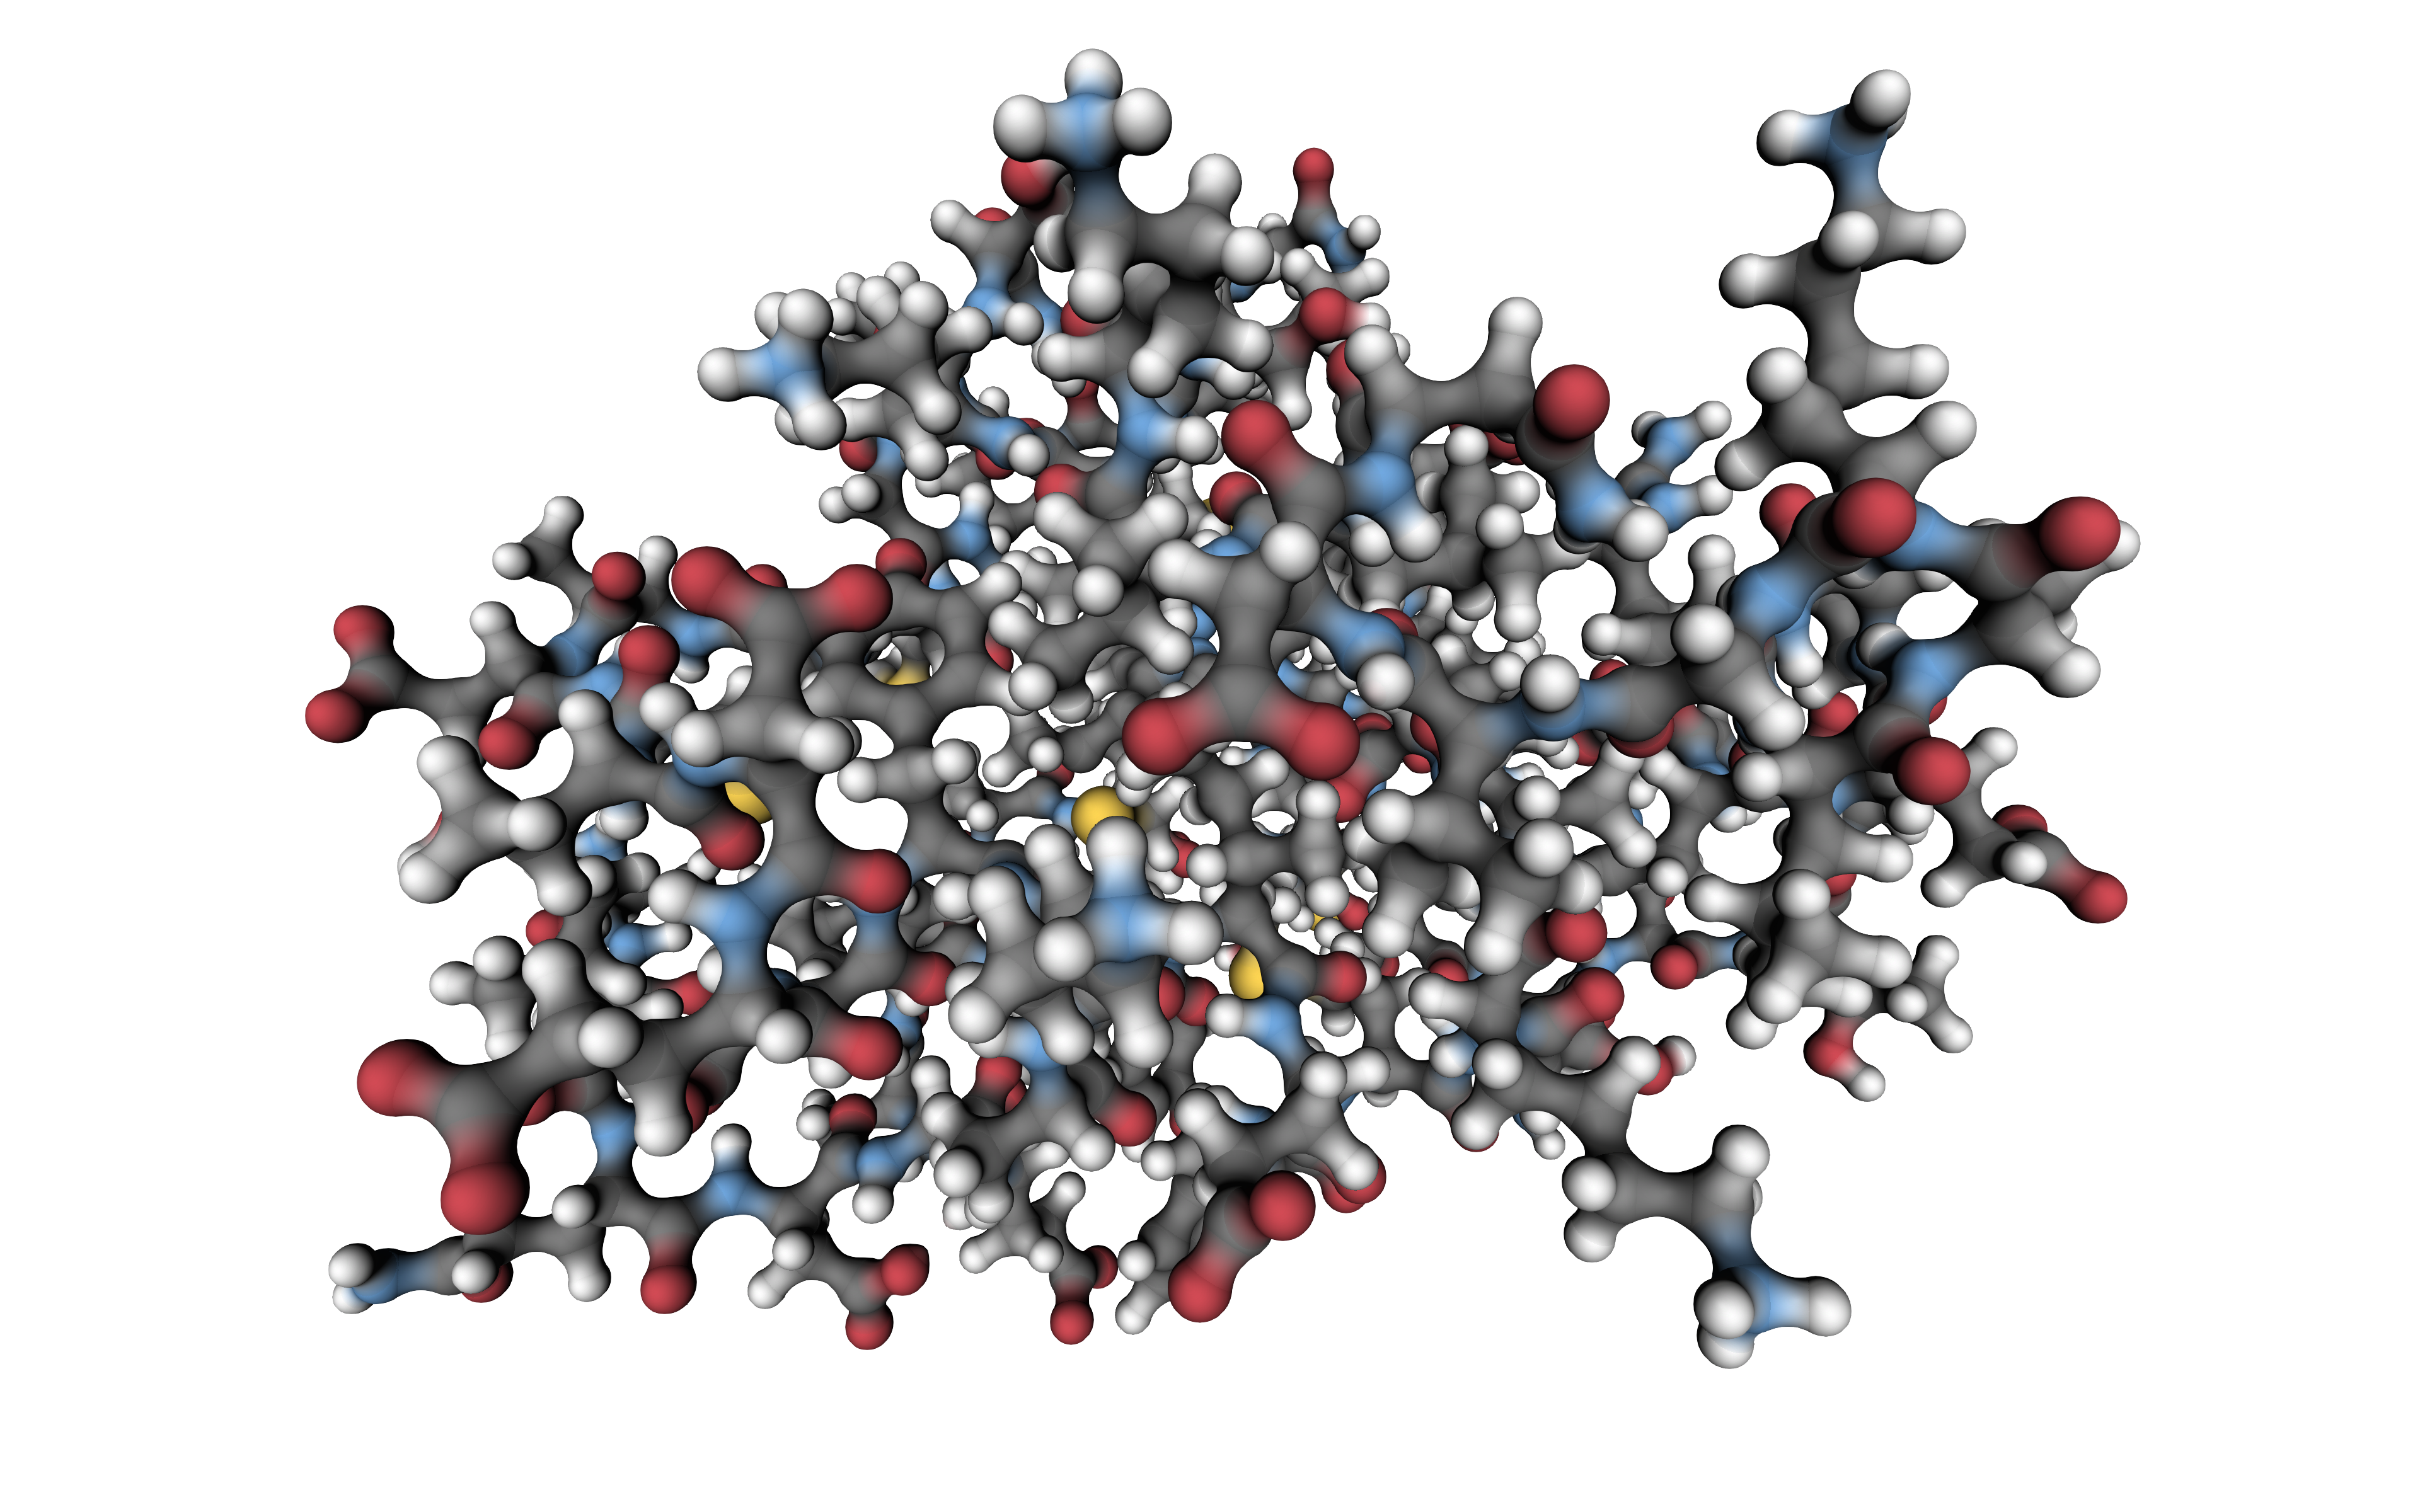
\includegraphics[width=\textwidth]{figures/ch1/1KX2}
		\caption{Illustration d'une protéine (1KX2, un mono-hème ferrocytochrome) produite avec le logiciel UnityMol~\cite{doutreligne2014unitymol}. Les atomes de carbone sont représentés en gris, ceux d'oxygène en rouge, d'hydrogène en blanc, et de soufre en jaune. Cette protéine est relativement petite, avec seulement 81 acides aminés, contre plusieurs centaines sur de nombreuses protéines ; de plus, ce mode de représentation, dans lequel les atomes ont un rayon inférieur à leur rayon de van der Walls, couramment utilisé, minimise l'occultation ; néanmoins, on constate qu'une très grande partie de la molécule est occulée par les atomes situés au premier plan. De surcroît, il s'agit ici d'une représentation \emph{in vacuo}, c'est-à-dire sans le solvant dans lequel une protéine se trouve généralement à l'état naturel.}
		\label{fig:1KX2}
	\end{figure}
    
	\subsection{Dynamique moléculaire}
	Une simulation de dynamique moléculaire consiste à simuler, par un calcul numérique, le comportement d'un système moléculaire dans le temps. Celui-ci est modélisé par un système de particules, avec généralement une particule par atome. Des formules mathématiques permettent de modéliser les différences forces qui s'appliquent à chaque particule, et ces forces sont intégrées avec un pas de temps pour déterminer le comportement dynamique du système.
    
	\subsection{Simulations interactives}
	Besoin de steering, etc.
	L'interaction avec une simulation de dynamique moléculaire présente plusieurs difficultés majeures. Tout d'abord, le nombre de cibles potentielles est très élevé, avec au minimum plusieurs centaines d'objets, généralement plusieurs dizaines de milliers, voire plusieurs centaines de milliers, dans les cas les plus extrêmes. Ces cibles étant confinées dans un espace relativement petit, il en resulte de plus une densité élevée, voire très élevée (selon le mode de représentation.
	 occultaton, vitesse, prévisibilité, etc.
	
	\section{Contrôle de l'espace aérien}
	La figure~\ref{fig:airtraffic} représente un écran de contrôle du trafic aérien. Les trajectoires des avions sont (normalement) légèrement courbées ou rectilignes, ce qui les rend particulièrement prévisibles, et donc facilite considérablement la tâche de sélection, comme nous le verrons en détail plus loin. Cependant, selon le niveau de zoom et la quantité d'informations contextuelles affichées sur l'écran, le niveau d'occultation peut devenir très important. La vitesse des cibles dépend également du niveau de zoom, mais dans une relation inverse : plus l'échelle est grande, plus les mouvements des avions seront lents sur l'écran.
	
	\subsection{Applications civiles}
	Quantitativement, un avion de ligne atterrit à environ 250~km/h et ne dépasse pas 1000~km/h. Ses changements de direction sont très progressifs, généralement de l'ordre de deux degrés par seconde. Ils sont peu fréquents et généralement prévisibles car ils ont pour but d'emprunter des couloirs aériens, ou des trajectoires d'approche imposées aux abords des aéroports.

	\paragraph{}
	Il n'en va toutefois pas de même pour les hélicoptères, qui peuvent faire demi-tour en environ quatre secondes, voire moins. Cependant, les modèles civils dépassent rarement les 300 km/h. La fréquence des changements de direction dépend considérablement de la mission, elle peut être faible pour un simple transport d'un point A vers un point B, auquel cas la trajectoire de l'hélicoptère va tendre vers la ligne droite, ou assez importante dans le cas d'un hélicoptère de police fournissant une assistance aérienne pendant une course-poursuite.
	
	\subsection{Applications militaires (surveillance de l'espace aérien)}
	Les aéronefs militaires présentent des caractéristiques beaucoup plus variables, dans des intervalles nettement plus grands. La vitesse d'un avion de chasse, par exemple, peut atteindre 3000~km/h~\cite{mig31}. Il est beaucoup plus difficile d'obtenir des données chiffrées sur la maœuvrabilité de tels engins, mais il est du moins clair qu'un avion de chasse moderne peut changer de direction beaucoup plus brutalement qu'un avion de ligne, et certaines sources non officielles font état de capacités de l'ordre de 35\textdegree{}/s pour les meilleurs. La fréquence maximale à laquelle un avion peut changer de direction est également difficile à connaître avec certitude, mais une simple observation d'une démonstration en vol permet d'estimer que cette valeur est, grossièrement, de l'ordre d'un changement par seconde environ~\cite{rafdemo}. Indépendamment des capacités techniques des avions militaires, leurs missions peuvent précisément imposer la recherche de l'imprévisibilité (par exemple pour éviter les tirs ennemis) ce qui n'est généralement pas le cas dans le civil.
	
	\begin{figure}[ht]
		\centering
		\includegraphics[width=\textwidth]{figures/AlFursan}
		\caption{La patrouille acrobatique émiratie \emph{Al Fursan}, avec ses trajectoires entremêlées mises en évidence par des traînées de fumée colorées. Crédit : The National UAE (\url{http://www.thenational.ae}).}
		\label{fig:alfursan}
	\end{figure}
	
	\paragraph{}
	De même, les hélicoptères militaires sont plus agiles que leurs homologues civils, sans qu'il soit aisé de quantifier cette différence. Comme pour les avions, leur comportement est susceptible d'être  Ils sont ausssi légèrement plus rapides, de quelques dizaines de km/h, notamment en piqué. Comme pour les avions, leurs missions impliquent souvent des trajectoires moins prévisibles.
	
	\paragraph{}
	Le cas des drones aériens, c'est-à-dire des aéronefs sans pilote embarqué (télécommandés ou autonomes) est peut-être le plus hétérogène. On trouve en effet des drones de très petite taille, mais aussi des modèles de plusieurs tonnes~\cite{reaper}. Leurs modes de sustentation sont très divers, leurs moyens de propulsion varient également, et de fait, leurs caractéristiques de vol sont extrêmement variables, des plus petits engins extrêmement manœuvrables jusqu'au plus gros, qui se comportent comme des avions. Au-delà de leurs caractéristiques de vol, certains drones sont délibérément conçus pour être utilisés en grandes quantités, en essaims~\cite{locust, alonso2016distributed, saska2014autonomous}, notamment pour submerger l'ennemi par le nombre. Cela implique une densité de cibles potentiellement très importante, avec les niveaux d'occultation qui en découlent.
	
	\begin{figure}[ht]
		\centering
		\includegraphics[width=\textwidth]{figures/swarm}
		\caption{Petit essaim de drones aériens. Crédit : \emph{International Business Times}.}
		\label{fig:swarm}
	\end{figure}
	
	\paragraph{}
	Dans une certaine mesure, le contrôle de la circulation des drones est également un enjeu pour le domaine civil, car ils peuvent évoluer (légalement ou non) près des aéroports. Cette pratique peut représenter un risque de sécurité, et des arrêtés ont été pris par le Ministère de l'écologie et du développement durable pour les prévenir, comme le rappelle notamment l'Union des Aéroports Français~\cite{dronesuaf}.
	
	\paragraph{}
	Les drones représentent aussi un risque sécuritaire civil généralisé :
	
	\begin{displayquote}
	C'est un mode d'action inédit contre des forces françaises. Le camp militaire d'Erbil, qui abrite des peshmergas et des commandos français au Kurdistan irakien, a été le théâtre d'une explosion sans précédent le 2 octobre dernier. Celle d'un drone, piégé par le groupe Etat islamique. Bilan : deux combattants kurdes tués, et deux commandos parachutistes de l'armée de l'air française grièvement blessés.
	
	[\ldots{}]
	
	« On ne peut pas faire grand-chose », constate avec amertume auprès de LCI Jean-Vincent Brisset, général de brigade aérienne. Ce directeur de recherche à l’IRIS l'assure : « C'est quelque chose d'assez terrifiant pour les services de sécurité. Il est horriblement compliqué de stopper un drone qui, par exemple, chercherait à s'attaquer à un responsable politique en plein discours. » Pour preuve, la scène surréaliste à laquelle avaient assisté ceux qui écoutaient Angela Merkel, il y a trois ans à Dresde. Durant son intervention, la chancelière avait observé l’atterrissage surprise d’un appareil au pied de la tribune.~\cite{brisset}

	
	\end{displayquote}
	
	\paragraph{}
	La surveillance de l'espace aérien concerne également divers types de missiles (de croisière, balistiques, etc.). Leurs caractéristiques détaillées sont généralement au moins aussi secrètes que celles des avions de chasse, mais on sait néanmoins qu'ils peuvent être à la fois hypersoniques (c'est-à-dire dépasser Mach~5) et manœuvrables à de telles vitesses~\cite{missiles}, comme le missile BrahMos-II dont une maquette est représentée sur la figure~\ref{fig:brahmos}.
	
	\begin{figure}[ht]
		\centering
		\includegraphics[width=\textwidth]{figures/brahmos-II}
		\caption{Maquette du missile hypersonique russo-indien BrahMos-II, en cours de développement. Crédit : Pakistan Defence (\url{http://defence.pk}).}
		\label{fig:brahmos}
	\end{figure}
	
	\paragraph{}
	En situation réelle, un espace aérien pourrait tout à fait contenir des véhicules et autres engins volants de tous les types sus-cités, des essaims de drones très manœvrables jusqu'aux missiles balistiques les plus rapides. Un système de contrôle interactif devrait donc être assez souple pour permettre la sélection de cibles de natures très différentes.
	On peut noter que les engins volants militaires ont vocation à chercher à éviter d'être détectés, soit en étant naturellement furtifs, soit en volant à très basse altitude et en tirant parti du relief naturel. Il en résulte qu'ils peuvent n'apparaître sur les écrans de contrôle que lorsqu'ils sont déjà très proches de lieux à protéger, et peuvent éventuellement disparaître de ces écrans, offrant une fenêtre temporelle restreinte pour l'interaction.
	
	\subsection{Observations}
	Qu'il s'agisse d'applications civiles ou militaires, cette tâche est critique, puisque de nombreuses vies sont en jeu. Selon l'application, il peut donc y avoir des contraintes fermes et spécifiques, soit sur le temps de sélection maximal acceptable (contrainte de temps-réel) soit sur le taux d'erreur, ou encore sur les niveaux de zoom, etc.

	Les systèmes de contrôle aérien dont nous avons connaissance sont tous en deux dimensions. Pour des engins volants, cela implique nécessairement une perte d'informations. Une technique de sélection suffisamment performante pourrait rendre envisageable l'utilisation d'un système en 3D. Cela permettrait par exemple de mieux déterminer si deux avions qui paraissent dangereusement proches dans le plan le sont réellement dans l'espace, ou de pouvoir choisir un objet parmi plusieurs évoluant aux mêmes coordonnées 2D, mais à des altitudes différentes, ou tout simplement d'avoir une meilleure représentation et perception générales de la situation.

	\begin{figure}[ht]
		\centering
		\includegraphics[width=\textwidth]{figures/Radar-Scope-ZSE}
		\caption{Écran de contrôle du trafic aérien. Toutes les informations, qui portent pourtant sur un espace tridimentionnel, sont représentées sur le même plan, avec une densité telle que certaines indications écrites sont illisible. Crédit : \emph{Bold Method}.}
		\label{fig:airtraffic}
	\end{figure}
	
	\section{Contrôle de l'espace maritime}
	\subsection{Enjeux}
	La figure~\ref{fig:channel} représente un écran de contrôle du trafic maritime en Manche. Fondamentalement, il s'agit d'un problème très similaire à celui du contrôle du trafic aérien, car il s'agit dans les deux cas de surveiller et organiser un espace fluide. Comme dans les airs, les enjeux sont à la fois militaires et civils. Les bâtiments militaires (\emph{a fortiori} s'ils sont potentiellement hostiles) doivent en effet être détectés le plus tôt possible et suivis tant qu'ils sont dans un espace d'intérêt défini, mais il faut également surveiller les bâtiments civils.
	
	\paragraph{}
	En effet, au-delà des activités commerciales normales qui font l'objet de contrôles douaniers, la mer abrite des activités illégales diverses, incluant tous types de trafics (contrebande, œuvres d'art, drogue, armes, êtres humains) mais aussi la piraterie ou des activités liées au terrorisme.
	Le fret maritime mondiale représentant près de 10 milliards de tonnes, on mesure l'ampleur et l'importance du défi à l'échelle planétaire~\cite{unctad}.
	
	
	\begin{figure}[ht]
		\centering
		\includegraphics[width=\textwidth]{figures/channel}
		\caption{Écran de contrôle représentant les navires utilisant le Système d'identification automatique (SIA) en Manche. Ce système n'étant obligatoire que sur les navires de jauge brute supérieure à 300 effectuant des voyages internationaux, ce n'est qu'une représentation partielle du trafic à cet instant. Crédit : \emph{Arlo Maritime}.}
		\label{fig:channel}
	\end{figure}
	
	\subsection{Difficultés}
	La plupart des navires se déplacent à la surface de l'eau. Par conséquent, leur représentation dans le plan sur un écran de contrôle n'implique généralement pas de perte d'information significative, contrairement au cas aérien. Toutefois, les sous-marins peuvent plonger à plusieurs centaines de mètres. S'ils représentent une très petite minorité des navires en circulation, leur détection revêt une importance militaire critique.
	
	\paragraph{}
	De fait, le problème de l'affichage planaire d'information tridimensionnelles demeure, même s'il est moins prégnant. Les navires sont en moyenne bien plus lents que les aéronefs, mais certains bateaux de type \emph{go-fast} peuvent dépasser les 150~km/h. Ces navires étant fréquemment utilisés par les trafiquants de drogue pour échapper aux garde-côtes, il est particulièrement important de pouvoir les détecter et les contrôler.
	
	\paragraph{}
	Comme souvent pour les tâches de ce type, la densité de cibles dépend du niveau de zoom, qui peut résulter d'un choix de l'utilisateur, ou d'une contrainte (l'obligation d'avoir en permanence une zone donnée affichée, par exemple). La densité peut donc varier et, potentiellement, être très élevée. Elle devient particulièrement problématique lorsque l'on souhaite afficher des informations contextuelles à propos des navires, ou d'un sous-ensemble de ceux-ci. Ces informations peuvent concerner le type du navire, son pavillon, son propriétaire, son équipage, son origine, sa destination (connue ou présumée) ses escales, sa cargaison, etc., ainsi que les éventuelles précédentes valeurs de toutes ces données.
	
	\paragraph{}
	Ces informations revêtent une importance particulière lorsqu'il est nécessaire aux autorités de faire la différence entre un bateau effectuant un simple voyage de plaisance et une embarcation susceptible d'être engagée dans une activité criminelle. Un groupe de \emph{speedboats} filant à vive allure vers une destination donnée peut tout aussi bien être un groupe d'amis en promenade qu'une bande de trafiquants de drogue. Il est donc nécessaire aux agents de contrôle de l'espace maritime de disposer d'un maximum d'informations le plus vite possible pour déterminer s'il est nécessaire d'ordonner l'interception de ces bateaux.
	
	\paragraph{}
	La figure~\ref{fig:lincoln} illustre un cas de forte densité locale de navires, avec des cibles de haute importance stratégique de surcroît. Près des ports, la densité peut être plus élevée encore, même si les navires concernés sont moins préoccupants pour les autorités. Il leur est toutefois nécessaire de garantir la circulation fluide et sûre de ces navires, et de veiller à ce que personne ne tire parti de cette forte densité à des fins illicites ou criminelles.
	
	\begin{figure}[ht]
		\centering
		\includegraphics[width=\textwidth]{figures/lincoln}
		\caption{Même dans des eaux relativement vides, la densité de navries peut être élevée localement. C'est généralement le cas quand un groupe aéronaval est présent, comme ici, avec le groupe aéronaval Abraham Lincoln, photographié en 2000. Il est de plus capital dans ce cas d'identifier clairement tous les navries présents, compte tenu de leur importance militaire. Crédit : \emph{Gabriel Wilson, via Wikimedia}.}
		\label{fig:lincoln}
	\end{figure}
	
	\section{Vidéo-surveillance}
	La vidéo-surveillance s'applique aussi bien aux foules dans les lieux publics ou sensibles qu'à la voirie, où peuvent circuler des véhicules de types divers. Un agent de sécurité en charge de visionner un flux de vidéo-surveillance pourrait avoir à sélectionner une personne, par exemple pour obtenir des informations sur celle-ci grâce à la reconnaissance faciale, ou un véhicule, pour les mêmes raisons, par exemple grâce à sa plaque d'immatriculation. Quelle que soit la nature de la cible, sa sélection pourrait avoir pour but de zoomer dessus, de verrouiller une caméra robotisée afin qu'elle la suive, ou de la désigner à des forces de sécurité sur le terrain pour qu'elles interviennent physiquement.
	
	\paragraph{}
	La vitesse d'un être humain à pied est inférieure à 45~km/h. Les changements de direction peuvent aller jusqu'au demi-tour, et leur fréquence est très variable selon la tâche accomplie. On peut supposer que cette fréquence est au plus de l'ordre de quelques Hz, en pratique généralement moins.

	\paragraph{}	
	Sur la voie publique, un véhicule motorisé n'est pas censé dépasser 130~km/h, exception faite de ceux qui enfreignent le code de la route. Mais, soit à cause de l'infraction en question, soit parce qu'ils l'enfreignent pour fuir après des délits ou crimes plus graves, ces véhicules-là peuvent justement faire l'objet d'une attention particulière de la part des forces de l'ordre. Dans ces cas-là, la vitesse d'un véhicule peut dépasser les 300~km/h~\cite{speeding}.
	
	Les changements de direction dépendent évidemment de la vitesse. En ville, à moins de 50~km/h, une automobile peut effectuer un virage à 90 degrés dans un laps de temps de l'ordre de la seconde si sa vitesse est réduite, mais elle est contrainte à des courbes beaucoup plus douces lorsqu'elle se déplace rapidement, par exemple sur une autoroute.
	
	La fréquence des changements de direction dépend également de la vitesse, tant pour des raisons physiques que du fait du tracé des trajets communément effectués. En milieu urbain dense, on peut considérer qu'un véhicule va changer de direction, de façon plus ou moins prononcée, à une fréquence de l'ordre de 0,1~Hz, sachant qu'en cas de nécessité, cette fréquence peut être nettement plus élevée.
	
	\paragraph{}
	En plus des piétons et des automobiles, la vidéo-surveillance s'applique à tous les véhicules et moyens de déplacement susceptibles d'être utilisés dans l'espace public : patins à roulettes, skateboards de tous types, bicyclettes, motocyclettes, etc. Les caractéristiques du mouvement de ces moyens de transport sont diverses, mais généralement comprises dans les intervalles formés par les piétons et les automobiles. Il est donc important qu'une technique de sélection puisse non seulement gérer les valeurs extrêmes de vitesse, d'angle et de fréquence de changements de direction, mais également les diverses combinaisons de ces valeurs qui peuvent se présenter simultanément.
	
	\paragraph{}
	Dans certains cas, par exemple au cours de manifestations publiques ou de concerts, les individus filmés peuvent devenir quasi statiques, mais très nombreux et confinés dans un espace réduit. Il en résulte une densité de cibles potentielles et un niveau d'occultation très élevés. Dans ces circonstances, la vidéo-surveillance 
	
	\begin{figure}[ht]
		\centering
		\includegraphics[width=\textwidth]{figures/crowdhk}
		\caption{Foule de manifestants à Hong-Kong. Mouvement très faible, mais densité très élevée. Crédit : \emph{Business Insider}.}
		\label{fig:crowdhk}
	\end{figure}
	
	\begin{figure}[ht]
		\centering
		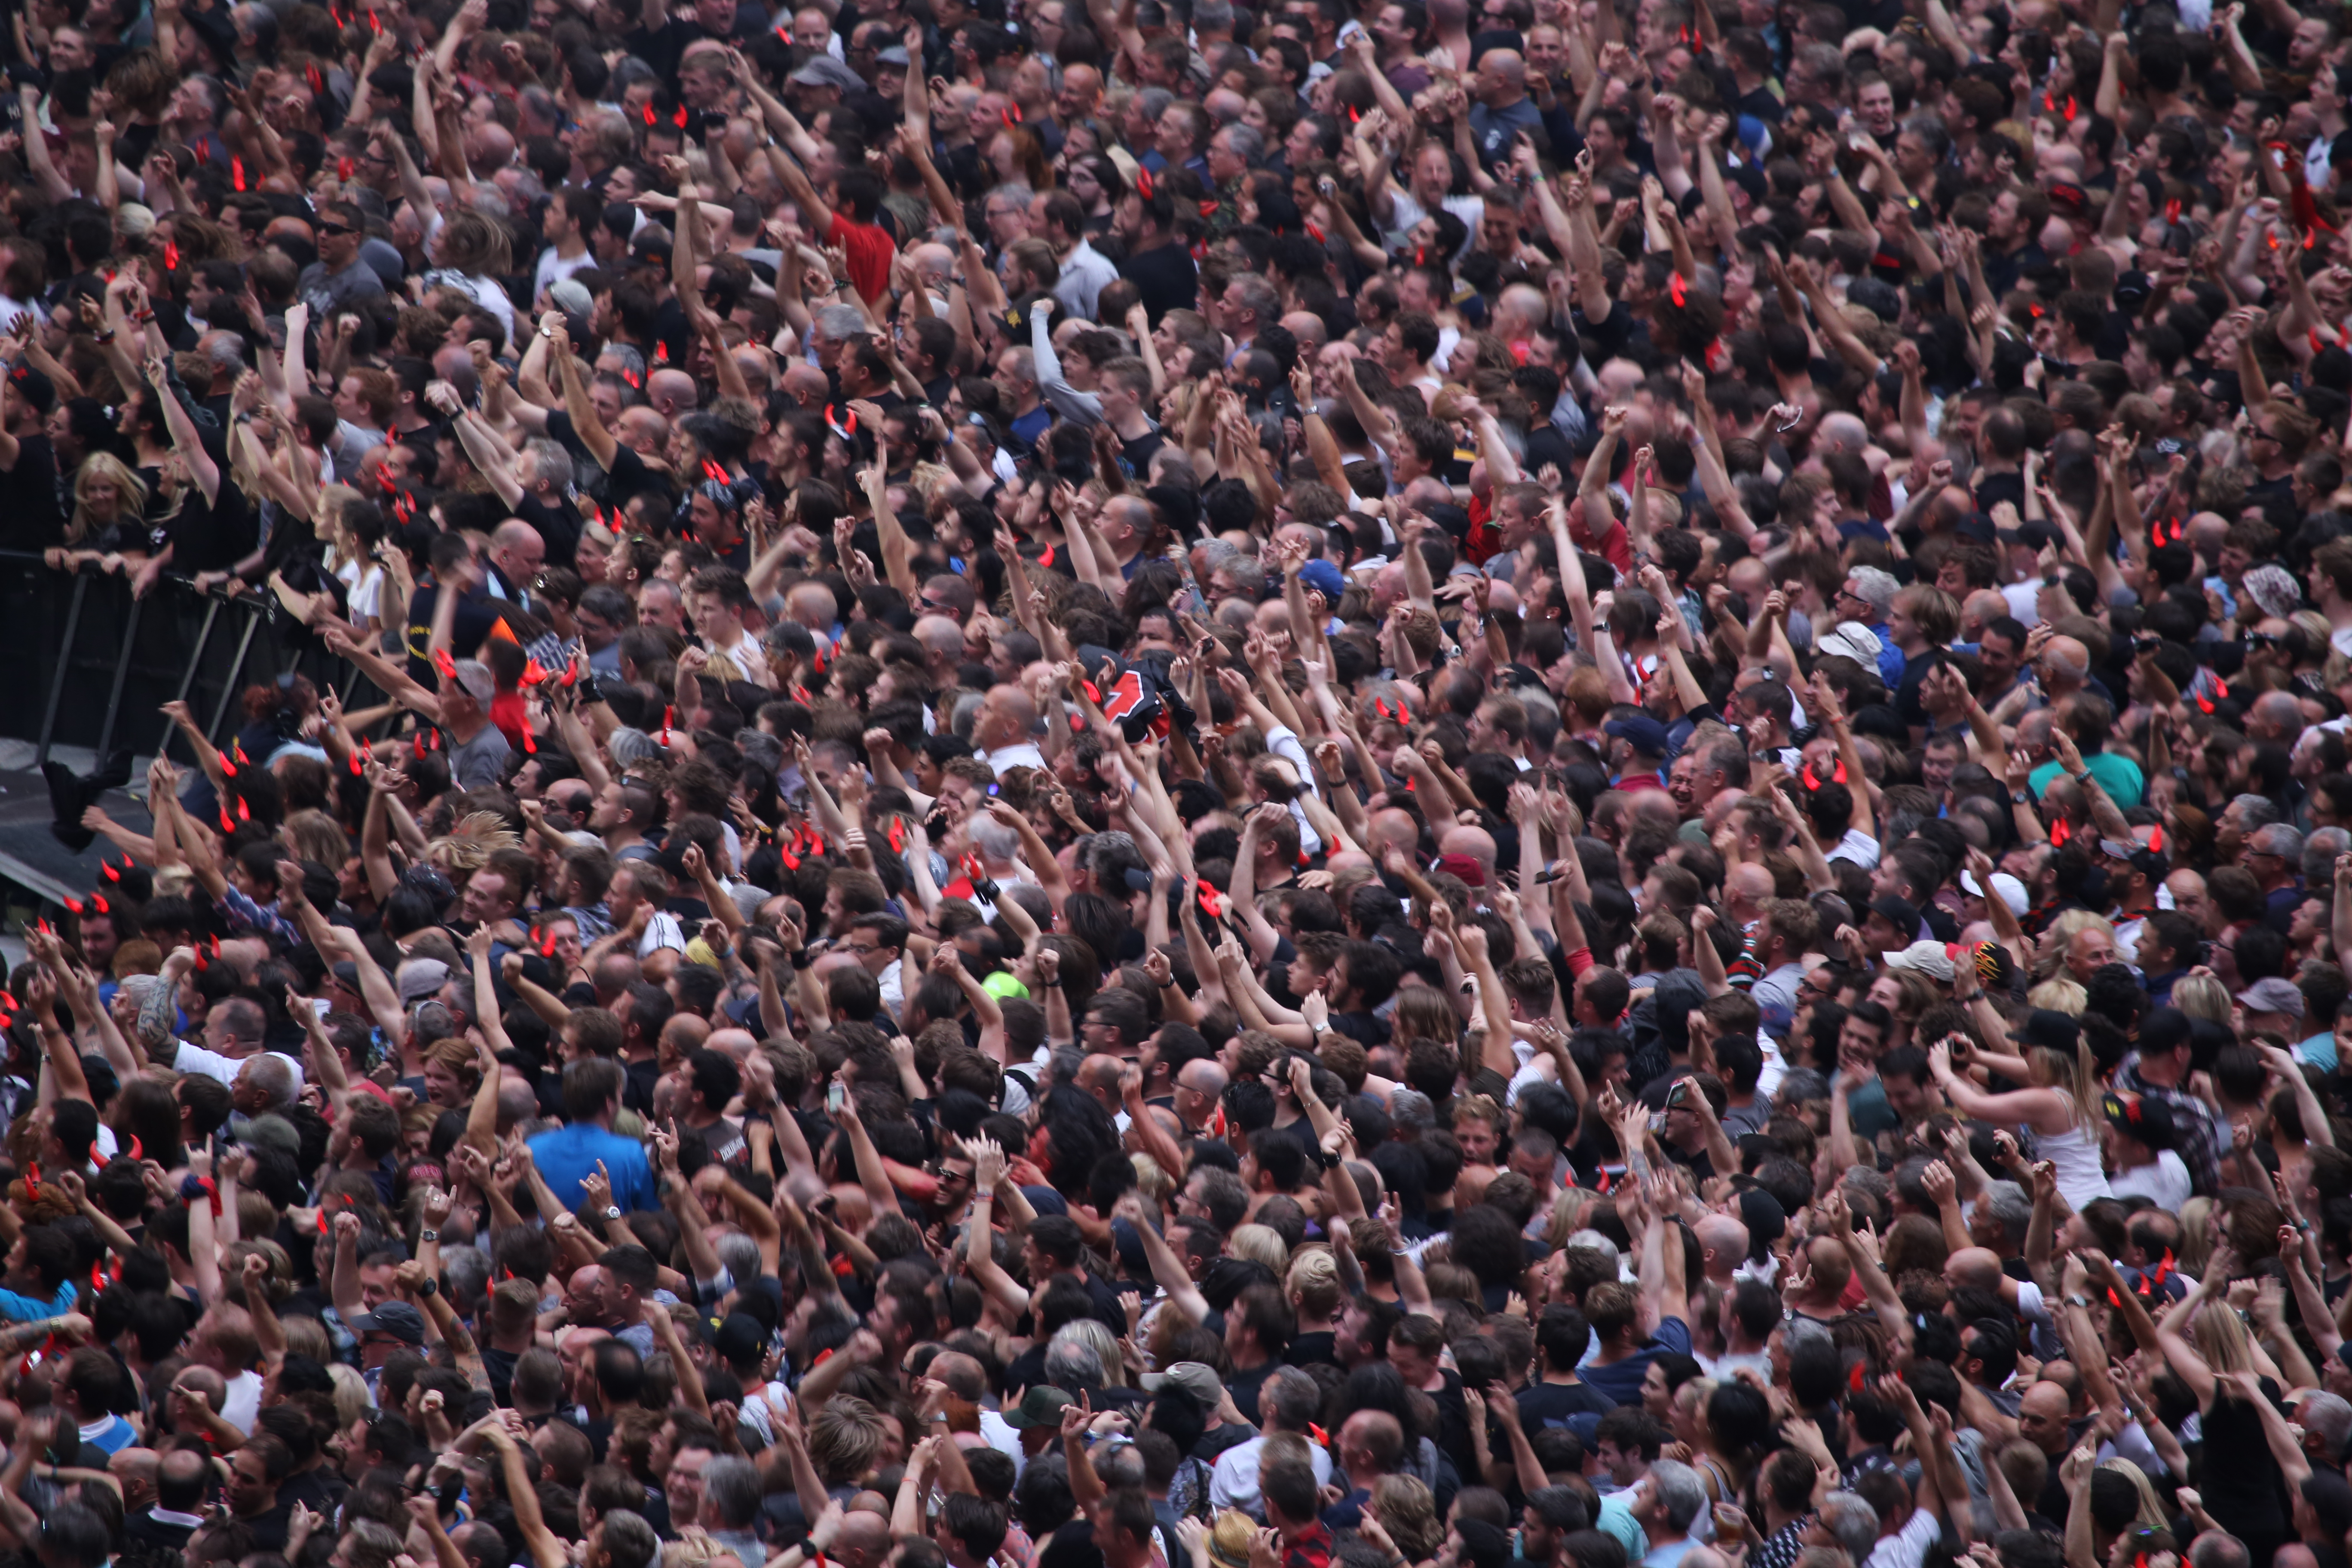
\includegraphics[width=\textwidth]{figures/crowdacdc}
		\caption{Foule à un concert du groupe AC/DC. Mouvement presque nul, mais densité extrêmement élevée. Crédit : \emph{SHP Online}.}
		\label{fig:crowdacdc}
	\end{figure}
	
	
	
	\section{Analyse de processus complexes}
	Mélange d'humains, de machines, espaces 3D, multiplicité d'objets, etc.
	
	\section{Retransmissions d'événements sportifs ou artistiques}
	Les retransmissions d'événements sportifs présentent un potentiel d'interactivité intéressant, nécessitant souvent la sélection de cibles mobiles. Il peut être utile, par exemple, de sélectionner un joueur de football pour afficher ses statistiques. Pour les mêmes raisons, un ballon ou une balle peut être une cible, de même que certains éléments du terrain de jeu, qui sont physiquement fixes mais peuvent être mobiles à l'écran du fait des mouvements de caméra. La nature du mouvement de ces cibles varie nécessairement d'un sport ou d'un jeu à l'autre.
	
	\paragraph{}
	Certains sports d'équipe comme le football, le hockey sur glace ou le basket-ball sont caractérisés par des cibles potentielles relativement nombreuses, mobiles, et dont les mouvements ne sont pas toujours très prévisibles. Les mouvements d'humains à pieds obéissent aux règles habituelles, mais dans un cadre sportif, ils peuvent être sur des patins à glace, des bicyclettes, des skis, etc., sans parler des sports hippiques ou mécaniques. Dans ces derniers cas, les mouvements sont souvent plus prévisibles, mais aussi nettement plus rapides, avec en plus une certaine tendance des cibles à être très proches les unes des autres, ce qui augmente la probabilité d'erreur de sélection.
	
	\paragraph{}
	Les divers projectiles utilisés en sports (balles, ballons, volants, palets, etc.) sont généralement beaucoup plus petits et rapides que les joueurs, ce qui en fait des cibles très difficile. D'un autre côté, il n'y a généraelement qu'un seul projectile de ce type par match, donc dans la mesure du possible, un raccourci dédié serait probablement une option préférable à l'utilisation d'une technique de sélection libre, fût-elle assistée.
	
	\begin{figure}[ht]
		\centering
		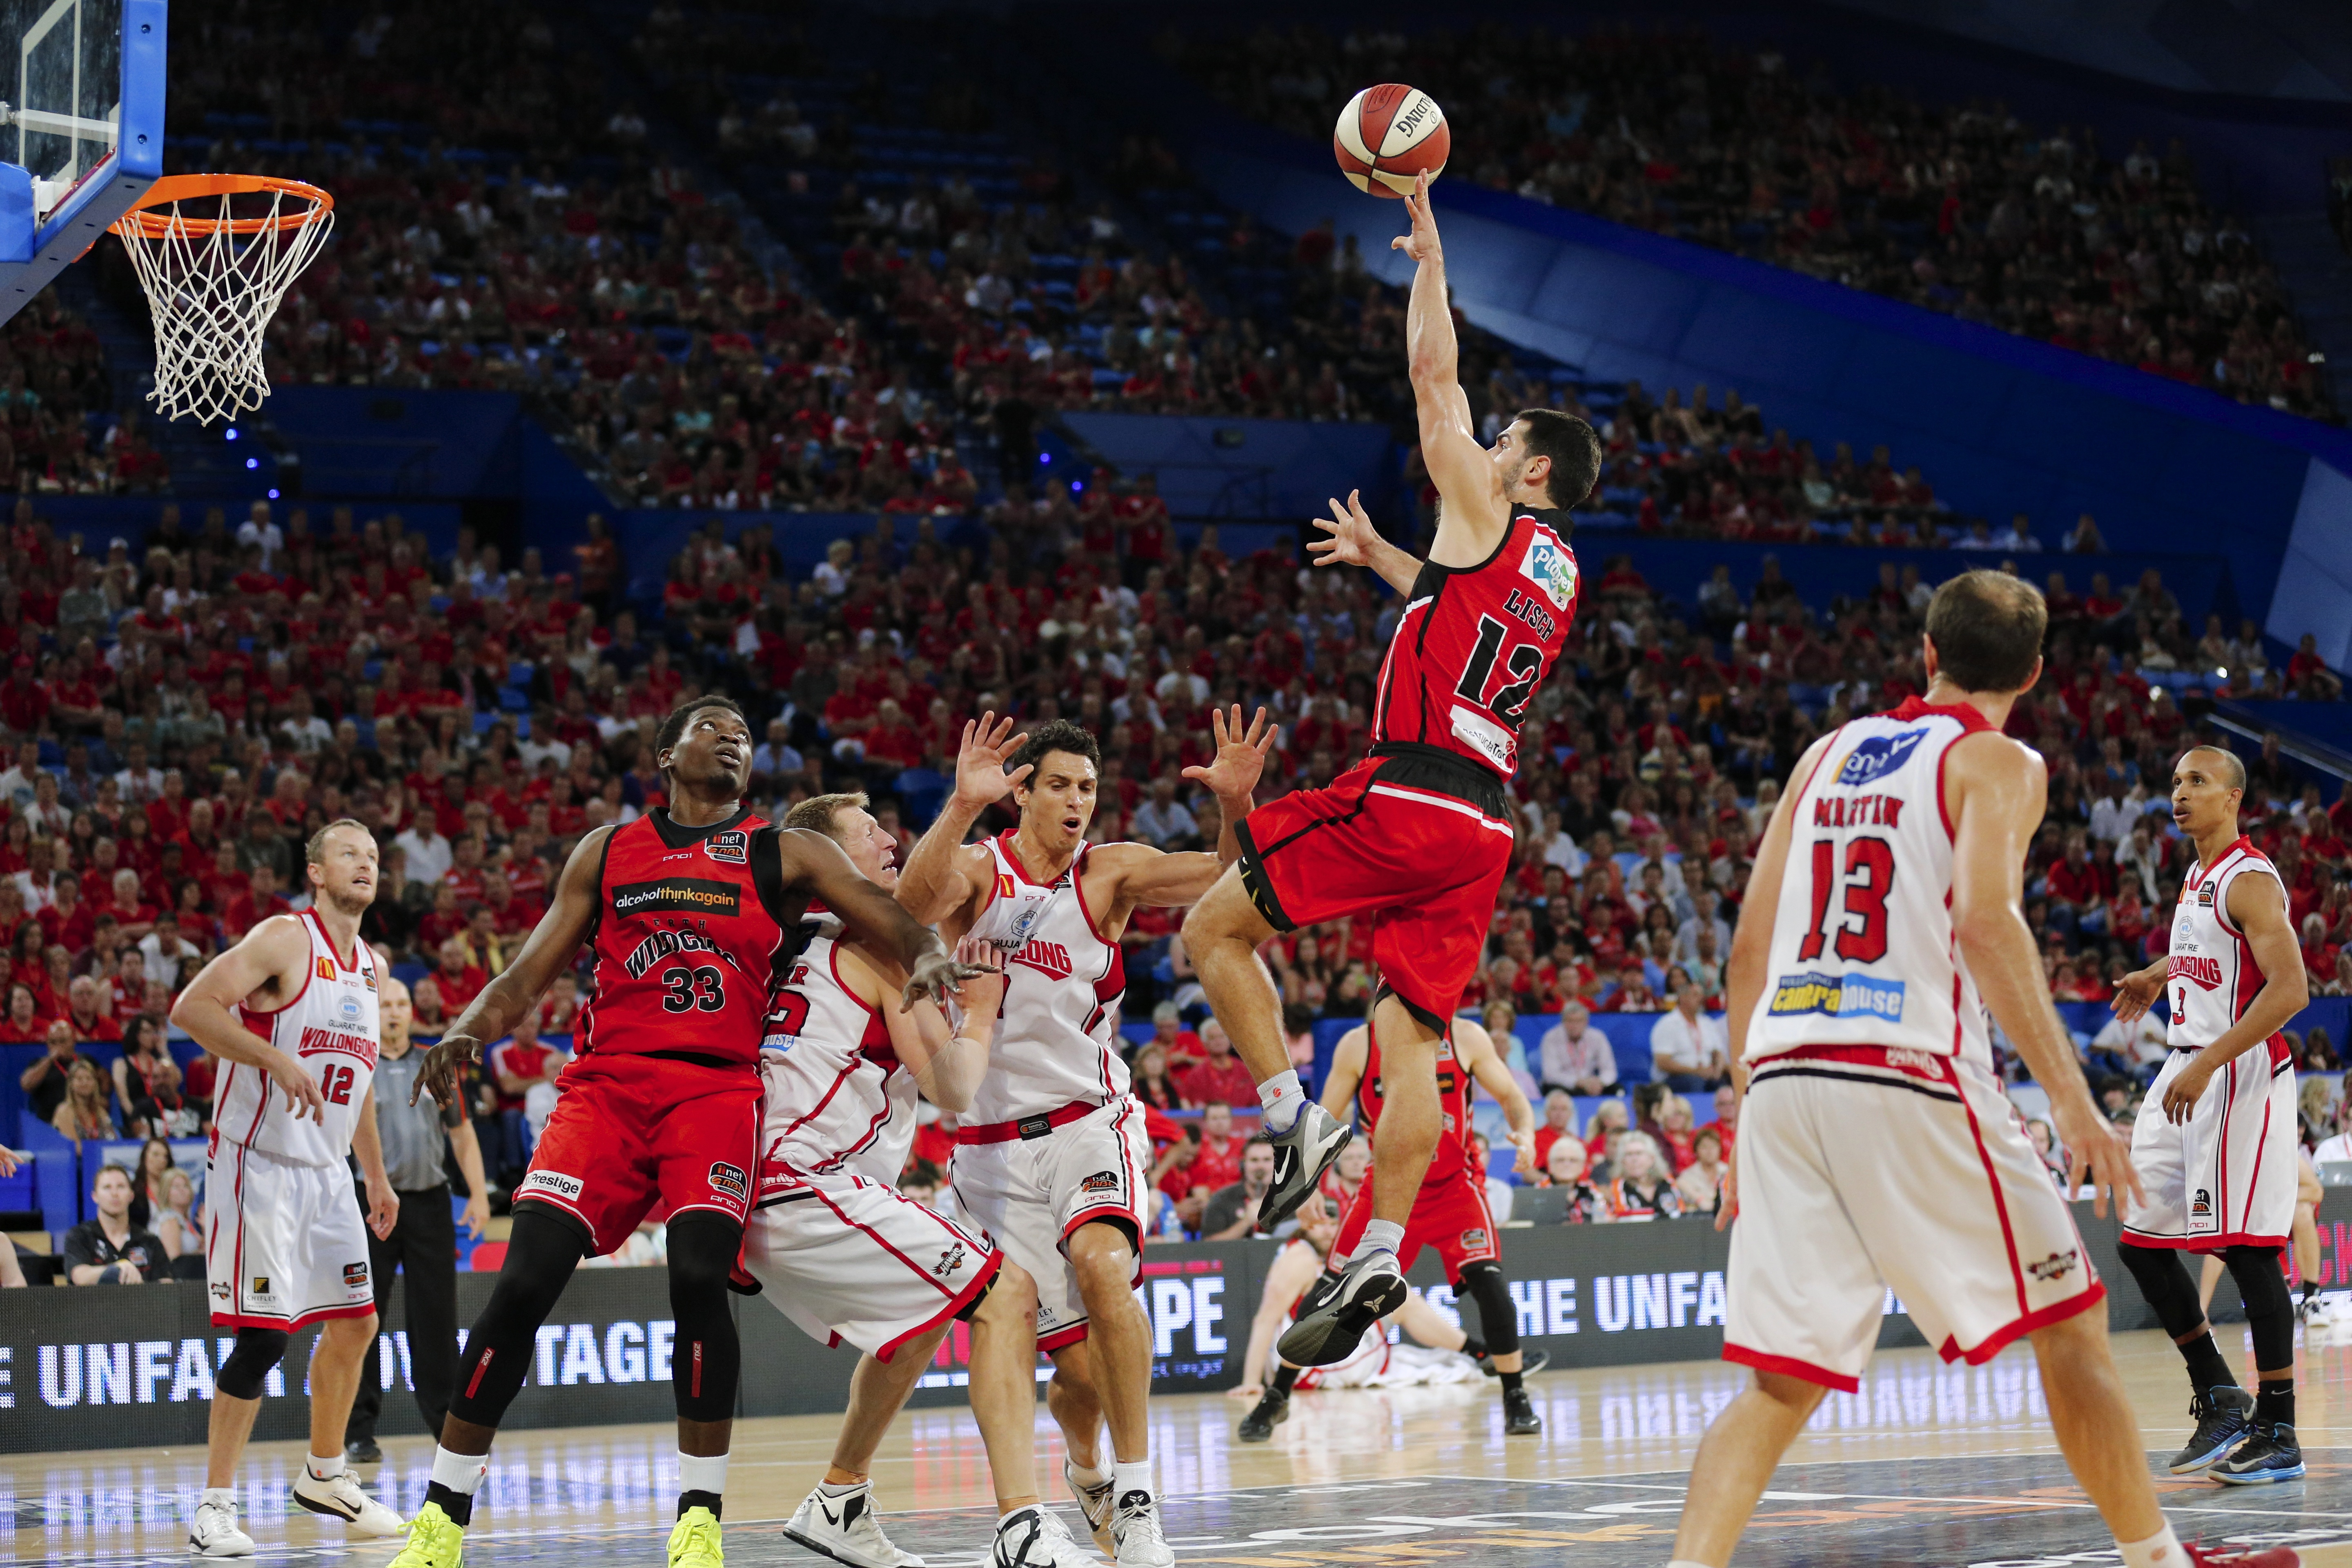
\includegraphics[width=\textwidth]{figures/basket}
		\caption{Match de basket-ball. Les joueurs sont peu nombreux, mais leurs mouvements sont vifs, horizontaux comme verticaux, et imprévisibles. Ils sont de plus très près les uns des autres et s'occultent mutuellement, \emph{a fortiori} quand ils sont filmés depuis le côté. Le ballon lui-même peut être une cible. Crédit : \emph{Weekend Notes}.}
		\label{fig:basketball}
	\end{figure}
	
	\section{Jeux vidéo}
	La sélection ou le pointage de cibles mobiles est une tâche que l'on retrouve dans de très nombreux jeux vidéo, appartenant à un nombre important de catégories. On peut notamment citer les jeux de tir (\emph{Fist-person Shooters}, ou FPS, comme \emph{Doom}, \emph{Counter-Strike}\ldots{}), les jeux de rôle d'action (\emph{Action role-playing games}, ou ARPG, comme \emph{The Witcher}, \emph{The Elder Scrolls}, voire \emph{Deus Ex}\ldots{}) les jeux de gestion (\emph{Anno}, \emph{Civilization}\ldots{}) ou de stratégie et tactique militaire (les catégories \emph{Real-time strategy} ou RTS, dans laquelle on trouve des jeux comme \emph{Starcraft} ou \emph{Age of Empires}, et \emph{Real-time tactics} ou RTT, avec \emph{Total War} ou \emph{World in Conflict}\ldots{}), les simulateurs de vol de combat (réalistes ou non, comme \emph{X-Plane}, \emph{IL-2 Sturmovik}, \emph{Elite: Dangerous}\ldots{}) ainsi que les jeux de type arène de bataille en ligne multijoueur (\emph{Multiplayer online battle arena}, ou MOBA, tels que \emph{League of Legends} ou \emph{DOTA~2}).
	
	D'un type de jeu à l'autre, la sélection de cibles varie à la fois du fait de la nature des cibles et parce que la tâche elle-même n'est pas vue de la même façon. Si elle est un élément essentiel des mécanismes du jeu dans certains genres, avec une valeur ludique propre, dans d'autres, elle est purement utilitaire, comme nous allons le voir dans les sous-sections suivantes.
	
	\subsection{Jeux de tir (FPS) et jeux de rôle d'action (ARPG)}
	Attendu que dans les FPS, la visée est précisément le cœur du jeu, et censée être difficile, les développeurs seraient probablement peu enclins à intégrer des techniques la facilitant, car cela diminuerait l'intérêt ludique de leur œuvre. Dans un jeu de rôle classique, c'est plutôt l'inverse. Les capacités du (des) personnage(s) contrôlé(s) par le joueur dépendent de l'expérience accumulée depuis le début du jeu, l'expérience étant ici une ressource précisément quantifiée, sous forme de points. Ces points sont ensuite investis dans des attributs (force, dextérité, endurance, intelligence\ldots{}) ou compétences (combat à mains nues, tir au fusil, persuasion, furtivité, magie de types divers\ldots{}). Souvent, les performances de visée d'un personnage dépendent uniquement de ses attributs et compétences, et non de la dextérité du joueur, qui n'a pas forcément besoin de désigner les cibles (le personnage les choisissant automatiquement) ou qui peut le faire pendant que l'action du jeu est en pause.
	
	\paragraph{}
	Mais il existe aussi une catégorie intermédiaire, les jeux de rôle d'action (ARPG). Les détails varient d'un jeu à l'autre, mais en général, le joueur est directement responsable des mouvements de ses personnages, mais les attributs et compétences du personnage ont une influence sur ses performances finales. Ce principe peut être mis en œuvre de diverses façons. En ce qui concerne le tir avec une arme (pistolet, arc, fusil\ldots{}) trois options, pas forcément mutuellement exclusives, sont couramment retenues :
	\begin{description}
		\item[Dispersion.] Quand les compétences de tir du personnage sont faibles, le réticule de visée est agrandi, ce qui indique au joueur que le cône de dispersion est large. À mesure que les compétences du personnage augmentent, le réticule et le cône se resserrent.
		\item[Perturbations.] Le curseur et le cône de dispersion peuvent être constants, mais ils bougent même lorsque le joueur ne touche pas à son périphérique de saisie. Celui-ci doit donc compenser ces mouvements pour viser correctement. À mesure que les compétences du personnage augmentent, ces mouvements diminuent, et peuvent finir par disparaître.
		\item[Recul.] Une arme qui tire un projectile a généralement un certain recul. Celui-ci n'a pas d'influence sur la précision du premier tir, mais sur tous les suivants. Dans un jeu vidéo, il est généralement simulé par un mouvement du curseur après le tir, habituellement vers le haut, avec en plus une composante horizontale, qui peut être aléatoire. On peut diminuer cet effet de recul quand les compétences du personnage croissent.
	\end{description}

	\paragraph{}
	Ces mécanismes permettent d'obtenir une difficulté de tir qui dépend du joueur, puisqu'il doit tout de même viser, mais les compétences du personnage jouent sur la difficulté de la tâche. On remarque qu'il s'agit toujours de gêner le joueur, de lui imposer un handicap qui diminue quand les compétences de ses personnages augmentent. Au final, le joueur reste borné par sa propre dextérité, comme dans un FPS classique.
	
	\paragraph{}
	Une autre technique, utilisée par les récents opus de la série \emph{Fallout} (désormais produite par Bethesda Studios) appelée \emph{Vault-Tec Assisted Targeting System}, ou V.A.T.S, consiste à arrêter ou considérablement ralentir le temps, pour permettre au joueur de désigner ses cibles, que le personnage attaquera ensuite automatiquement. Cette opération se fait en échange de << points d'action >>. L'inconvénient majeur de cette solution est la perte du temps-réel, et l'impact négatif sur l'immersion qui y est associé. De plus, le caractère automatique de l'attaque, une fois les cibles désignées, rend l'opération totalement indépendante de la dextérité du joueur, ce qui d'une part est une déviation du paradigme de l'ARPG, et d'autre part peut diminuer l'intérêt ludique du combat.
	
	\paragraph{}
	On pourrait imaginer, à la place ou en complément de ces approches, d'apporter au joueur une assistance à la visée. Une telle technique d'aide à la sélection devrait être paramétrable dans son << intensité >>, c'est-à-dire qu'il devrait lui être possible d'apporter au joueur une assistance plus ou moins prononcée, selon un paramètre donné. Ce paramètre pourrait être (dérivé de) la compétence de tir du personnage. Ainsi, un joueur contrôlant un personnage expert en tir serait capable d'abattre des cibles très difficiles, conformément à l'image du personnage telle qu'elle est véhiculée par le jeu, mais le joueur resterait l'acteur principal de l'opération, sans ralentissement ou suspension du temps.
	
	\begin{figure}[ht]
		\centering
		\includegraphics[width=\textwidth]{figures/f4vats}
		\caption{Dans l'ARPG \emph{Fallout 4}, le système V.A.T.S. permet ici au joueur de cibler tranquillement la tête de cette créature, pendant que le temps est ralenti. Le tir aura une probabilité de succès de 77~\%{}, dérivée des compétences de tir du personnage contrôlé, et des circonstances du combat à cet instant précis. Crédit : \emph{Spider's Web}.}
		\label{fig:f4vats}
	\end{figure}
	
	\subsection{Jeux de gestion, de stratégie (RTS) et de tactique (RTT)}
	Dans ce que nous appellerons, pour simplifier, les jeux de gestion (en y incluant les RTS et RTT) le but est de mener un organisme (d'une petite entreprise à une civilisation) vers la prospérité, ou une armée vers la victoire. Ces genres mettent l'accent sur la réflexion tactique et stratégique, la gestion des ressources naturelles et humaines, l'organisation logistique, l'utilisation astucieuse du terrain, l'art de la feinte, etc. S'il est fréquemment nécessaire de sélectionner des cibles dans ces jeux, ce n'est pas une fin en soi, ou un objectif conçu comme ayant une valeur ludique. Il s'agit de sélectionner des unités amies pour leur donner des instructions, ou des unités ennemies pour les désigner comme cibles à attaquer. Au contraire, la tâche de sélection fait perdre du temps au joueur, du temps qui pourrait être utilisé pour organiser ses resources et forces, ou tout simplement pour réfléchir.
	
	\paragraph{}
	Par conséquent, une technique de sélection facilitant cette tâche autant que possible serait probablement bénéfique en recentrant ces jeux sur leurs cœurs. Dans les jeux de gestion, les cibles peuvent être extrêmement nombreuses. Dans \emph{Cossacks~2: Napoleonic Wars}, par exemple, une bataille peut engager jusqu'à 64~000 unités, et la situation devient suffisamment assez délicate à gérer pour pousser les joueurs à mettre le jeu en pause, le temps de donner des instructions aux unités~\cite{cossacks2}. Il est évident que si cette solution est acceptable (quoique loin d'être idéale) dans un jeu opposant une intelligence artificielle au joueur humain, elle vient beaucoup plus gênante dans un contexte multijoueur.
	
	
	\begin{figure}[ht]
		\centering
		\includegraphics[width=\textwidth]{figures/cossacks2}
		\caption{Exemple d'une partie du RTS \emph{Cossacks~2: Napoleonic Wars}, avec de nombreuses unités, très proches les unes des autres. Au nombre et à la densité s'ajouteront, pendant la bataille, le mouvement, le désordre et le mélange avec des unités ennemies. Crédit : \emph{Worth Playing}.}
		\label{fig:cossacks2}
	\end{figure}
	
	\begin{figure}[ht]
		\centering
		\includegraphics[width=\textwidth]{figures/eveonline}
		\caption{Énorme bataille dans le jeu \emph{EVE Online}. Le nombre précis d'unités est inconnu, mais chaque point rouge ou orange représente un vaisseau ou un drone, donc une cible potentielle. Au-delà du nombre extrêmement important de cibles, ce cas présente la difficulté d'être en trois dimensions, ce qui complique la saisie et implique un haut niveau d'occultation, en particulier pour les petits vaisseaux situés derrière un vaisseau capital ou de grande taille. Crédit : \emph{EVE Online Community}.}
		\label{fig:eveonline}
	\end{figure}
	

	\subsection{Arènes de bataille en ligne multijoueur (MOBA)}
	Les jeux de type MOBA sont caractérisés par un petit nombre de cibles (de l'ordre de quelques dizaines, tout au plus) rapides et imprévisibles.

	\paragraph{}
	Le \emph{wiki} du jeu \emph{DOTA~2} fournit des informations très précises sur les caractéristiques de mouvement des unités principales~\cite{dota2}.	 Celles-ci sont reproduites dans le tableau~\ref{tab:dotamoves}.
	
	\newcommand{\newrow}{\bigstrut[t] \\ \hline}
	\begin{table}[ht]
		\centering
		\begin{tabular}{ p{0.25\textwidth} c c }
		Héros				&	Temps de demi-tour (180°)	&	Vitesse (unités arbitraires)	\newrow
		Lifestealer		&	0.094 s				&	315						\newrow
		Shadow Fiend		&	0.094 s				&	315						\newrow
		Faceless Void		&	0.094 s				&	300						\newrow
		Batrider			&	0.094 s				&	290						\newrow
		Bristleback		&	0.094 s				&	290						\newrow
		Phoenix			&	0.094 s				&	285						\newrow
		Earthshaker		&	0.105 s				&	310						\newrow
		Magnus			&	0.118 s				&	315						\newrow
		Storm Spirit		&	0.118 s				&	285						\newrow
		Luna				&	0.157 s				&	335						\newrow
		Gyrocopter			&	0.157 s				&	315						\newrow
		Keeper of the Light	&	0.188 s				&	335						\newrow
		Pugna				&	0.188 s				&	330						\newrow
		Leshrac			&	0.188 s				&	325						\newrow
		Skywrath Mage		&	0.188 s				&	325						\newrow
		Lich				&	0.188 s				&	315						\newrow
		Outworld Devourer	&	0.188 s				&	315						\newrow
		Enchantress		&	0.236 s				&	335						\newrow
		Lone Druid			&	0.236 s				&	325						\bigstrut[t] \\
		\end{tabular}
		\caption{Caractéristiques de mouvement des personnages les plus vifs du MOBA \emph{Dota~2}.}
		\label{tab:dotamoves}
	\end{table}
	
	\begin{figure}[ht]
		\centering
		\includegraphics[width=\textwidth]{figures/lol2}
		\caption{Exemple d'une partie d'un MOBA, le jeu \emph{League of Legends~2}, avec quelques personnages. Crédit : \emph{Dota Geeks}.}
		\label{fig:lol2}
	\end{figure}
	
	\begin{figure}[ht]
		\centering
		\includegraphics[width=\textwidth]{figures/dota2}
		\caption{Exemple d'une partie d'un MOBA, le jeu \emph{DOTA~2}. Les caractéristiques de ses personnages les plus vifs sont dans le tableau~\ref{tab:dotamoves}.}
		\label{fig:dota2}
	\end{figure}
	
	
	\section{}    
	Les tendances observées sur les cibles statiques demeurent, à savoir que la difficulté de la tâche augmente quand la distance entre la cible et le pointeur augmente, ou quand la taille de la cible diminue. Mais l'influence du mouvement de la cible empêche d'appliquer la loi de Fitts. Certes, la difficulté de la tâche augmente aussi avec la vitesse, [ref-mec-interact?] cependant, si la nature du mouvement a une importance cruciale, celle-ci demeure peu étudiée.
    
    
    
    
 The
difficulty of the selection increases while (1) target size decreases,
(2) target velocity increases and (3) target density increases. The
selection is even more difficult in 3D environments (filmed or synthetic
environments) because a target of interest can be occluded
by others targets. Selecting someone in crowds with a surveillance
video system is an example of a dense environment with small targets
and occlusion. In some cases, like in action sport footage, both
the objects of interest and the camera can move. Target movements
become unpredictable, and the selection is even more difficult.
In this context, as Hasan et al. [3] wrote, for completing the
selection ”the user must continually track the target and simultaneously
plan to move the cursor over it”. This underscores the key
point of the technique we propose here. Since the user follows the
target for selecting it, the Hook technique tracks the cursor behavior
for assisting the selection. Indeed, observing the history of cursor
displacements, and the history of distances between each target and
the cursor, the system can estimate which target is tracked, and then
propose a selection to the user who just has to validate it. In other
words, the user follows the target of interest, and the system will
know which target it is.
This paper presents the implementation of this technique, and
two experiments which investigate its performance. Hook has been
compared to the basic pointing (non assisted pointing), and to Bubble
cursor [2, 8], for the case of 3D object selection. The first evaluation
involves a desktop configuration, in which pointing is done
on a standard screen with a mouse. The second evaluation involves
an immersive configuration in which pointing is done with a 3dof
(degrees-of-freedom) device. Both evaluations highlight the bene-
fits of this new interaction technique for selecting moving targets in
a 3D environment. More than simply improving the pointing time,
Hook drastically decreases the error rate and allows pointing targets
in high density environments, with high velocity targets that are not
possible to capture with other techniques.


	
		

\clearpage

%!TEX root = these.tex

\chapter[État de l'art des techniques de sélection]{État de l'art des techniques de sélection}
\minitoc
\label{chap2}
\cleardoublepage

\section{Introduction}
	\subsection{Pointage, sélection et loi de Fitts}
	Le pointage et la sélection de cibles sont de vieux problèmes. Si les cas qui nous intéressent, énumérés dans le chapitre précédent, présentent des difficultés particulières, de nombreuses techniques existent déjà et certaines d'entre elles tiennent compte d'une partie de ces difficultés. L'on peut faire remonter l'histoire de la recherche sur le pointage au moins jusqu'à la loi de Fitts~\cite{fitts1954information}. Celle-ci fut établie notamment grâce à une expérience simple, dans laquelle on demandait aux sujets de toucher certaines zones à l'aide d'un stylet, comme illustré par la figure~\ref{fig:fitts}, et détaillé par sa légende.
	
	\begin{figure}[H]
		\centering
		\includegraphics[width=\textwidth]{figures/ch2/fitts}
		\caption[Expérience de Paul M. Fitts.]{Illustration de la première expérience ayant mené Paul Fitts a la découverte de sa loi. Deux triplets de plaques étaient séparés d'une certaine distance. Les sujets devaient, avec leur stylet \og tapoter \fg{} alternativement les deux plaques centrales de chaque triplet, hachurées sur ce schéma, sans toucher les plaques adjacentes. On pouvait faire varier la largeur des plaques ciblées, ainsi que la distance entre elles. Crédit : Paul M. Fitts~\cite{fitts1954information}.}
		\label{fig:fitts}
	\end{figure}
	
	Paul M. Fitts a donc pu déduire de cette étude la loi qui porte son nom, et que l'on peut décrire par les équations~\ref{eq:fitts} et~\ref{eq:fittsID}.
	
	\begin{equation}
		\label{eq:fitts}
		MT = a + bID
	\end{equation}
	
	\begin{equation}
		\label{eq:fittsID}
		ID = \log_2\left(\frac{2D}{W} \right)
	\end{equation}
	
	Dans l'équation~\ref{eq:fitts}, $MT$ représente le temps de mouvement, $a$ et $b$ sont des constantes déterminées empiriquement. Dans l'équation~\ref{eq:fittsID}, $ID$ représente l'indice de difficulté, $D$ représente l'amplitude du mouvement, c'est-à-dire la distance entre la cible et le point de départ du mouvement, tandis que $W$ représente la largeur de la cible. La partie la plus intéressante de cette équation est l'indice de difficulté. C'est la seule partie variable, et c'est celle qui, comme son nom l'indique, détermine la difficulté de la tâche. Cet indice est aisé à comprendre intuitivement : plus l'amplitude du mouvement nécessaire est grande, plus la tâche sera difficile ; plus la largeur de la cible est grande, plus la tâche sera facile.
	
	Pour l'indice de difficulté, MacKenzie propose une formulation de l'indice de difficulté dite de Shannon, inspirée de la théorie de l'information proposée par ce dernier~\cite{mackenzie1989note}. Cette formulation est fournie dans l'équation~\ref{eq:shannon}.
	
	\begin{equation}
		\label{eq:shannon}
		ID = \log_2\left(\frac{D}{W} + 1\right)
	\end{equation}
	
	\subsection{Extensions de la loi de Fitts}
	L'étude de Paul M. Fitts portait sur un dispositif mécanique simple, mais sa loi s'applique aussi bien aux périphériques de saisie classiques (souris, \emph{joysticks}, etc.)~\cite{card1978evaluation}. Mieux, alors qu'elle fut d'abord énoncée pour des mouvements sur une seule dimension, elle loi s'étend aisément au plan~\cite{card1978evaluation, mackenzie1992extending}, éventuellement en tenant compte de la forme de la cible~\cite{accot2003refining}, ou même à l'espace tridimensionnel~\cite{murata2001extending}. On peut également généraliser la loi de Fitts pour modéliser des tâches de tracé de trajectoires~\cite{accot1997beyond, accot1999performance}.
	
	Bien que la loi de Fitts soit d'une élégante simplicité et d'une utilité évidente pour modéliser les performances de sélection, de nombreuses formulations plus ou moins différentes existent, et leurs mérites respectifs font débat~\cite{casallas2015prediction}. Certaines formulations peuvent, par exemple, tenir compte de l'angle $\theta$ entre le vecteur qui va du curseur à la cible et un vecteur horizontal orienté vers la droite (cf. la figure~\ref{fig:theta}). C'est le cas de la formulation de~\cite{murata2001extending} exposée dans l'équation~\ref{eq:murata}.
	
	\begin{equation}
		\label{eq:murata}
		ID = \log_2\left(\frac{D}{W} + 1\right) + c \sin \theta
	\end{equation}
	
	\begin{figure}[ht]
		\centering
		\includegraphics[width=\textwidth]{figures/ch2/theta}
		\caption[Fitts et $\theta$]{Angle $\theta$ pris en compte par~\cite{murata2001extending} dans une version étendue de la loi de Fitts, présentée dans l'équation~\ref{eq:murata}. Le disque rouge représente le curseur, tandis que le rectangle vert représente la cible, située à une distance $D$ du curseur, avec sa largeur $W$ et sa hauteur $H$. Crédit : \cite{casallas2015prediction}.}
		\label{fig:theta}
	\end{figure}
	
	D'autres versions tiennent compte simultanément de la forme de la cible et de cet angle $\theta$~\cite{appert2008evaluation, grossman2004pointing}.
	
	\subsection{Loi de Fitts et cibles mobiles}
	La recherche sur la loi de Fitts appliquée aux cibles mobiles, comparativement aux travaux sur les cibles statiques, est très pauvre~\cite{casallas2015prediction}. Elle n'est pas inexistante~\cite{jagacinski1980test, hoffmann1991capture, hajri2011moving} mais très limitée, et elle s'intéresse rarement à la nature du mouvement des cibles, surtout quand ce mouvement est imprévisible.
	
	De fait, les modèles développés dans les travaux de Jagacinski \emph{et al.}~\cite{jagacinski1980test} ou d'Al Harji \emph{et al.}~\cite{hajri2011moving}, par exemple, font l'hypothèse de cibles de vitesse et de direction constantes. La loi de Fitts étendue par Jagacinski \emph{et al.} est présentée dans l'équation~\ref{eq:jagacinski}, où $CT$ est le temps de sélection, $D$ et $W$ sont toujours la distance à la cible et sa largeur, $V$ est la vitesse de la cible, tandis que $c$, $d$ et $e$ sont des constantes réelles.
	
	\begin{equation}
		\label{eq:jagacinski}
		CT = c + dD + e(V + 1) \left(\frac{1}{W} - 1\right)
	\end{equation}
	
	Les travaux d'Al Harji \emph{et al.}~\cite{hajri2011moving} vont plus loin en tenant compte de la direction de la cible. Les auteurs ont développé deux modèles basés sur ce principe. Le premier est défini par l'équation~\ref{eq:hajriC2}, où $\vec{F}$ est un vecteur déterminé empiriquement, $\vec{D}$ est le vecteur distance entre le curseur et la cible, $\vec{V}$ est le vecteur de vélocité de la cible, et $\vec{R} = \frac{1}{2} \begin{pmatrix}
	W \\ H \\
	\end{pmatrix}$.
	
	Le second est défini par l'équation~\ref{eq:hajriVW}, où $f_{W'}(\theta)$ est un paramètre empirique dépendant de $\theta$, l'angle formé par la direction du mouvement de la cible et l'horizontale. De même $K$ est un paramètre empirique. $D$ est la distance entre le curseur et la cible, $V$ est la vitesse de la cible, et $W'$ est sa largeur dans la direction du mouvement.
	
	\begin{equation}
		\label{eq:hajriC2}
		ID_{C2} = \log_{2}\left(\abs*{\vec{F} \frac{\vec{D}+\vec{V}}{\vec{R}-\vec{V}}} + 1 \right)
	\end{equation}
	
	\begin{equation}
		\label{eq:hajriVW}
		ID_{VWtW'\theta} = \log_{2}\left( f_{W'}(\theta) \left( \frac{D \pm \frac{V}{K}}{\frac{W'}{2} - \frac{V}{K}} \right) \right)
	\end{equation}
	
	Les corrélations entre ces indices de difficulté et les temps de sélection mesurés par Al Hajri \emph{et al.} sont présentées sur la figure~\ref{fig:holdID}, où l'on observera qu'elles sont très fortes. Néanmoins, ces travaux ne portent que sur des cibles dont la vitesse et la direction sont constantes.
	
	\begin{figure}[H]
		\centering
		\includegraphics[width=\textwidth]{figures/ch2/holdID}
		\caption[Indice de difficulté en fonction de la nature du mouvement et temps de sélection]{Temps de sélection en fonction des indices de difficulté développés par Al Harji \emph{et al.} Les deux indices sont très fortement corrélés avec les temps de sélection mesurés (sans aucune assistance à la sélection). Crédit : \cite{hajri2011moving}.}
		\label{fig:holdID}
	\end{figure}
	
	D'autres travaux s'attachent à développer des techniques de sélection de cibles mobiles « quelconques » --- c'est-à-dire de direction et de vitesse potentiellement changeantes --- sans nécessairement s'attarder sur les aspects théoriques~\cite{hasan2011comet, ortega2013hook}, et donc sans chercher à étendre la loi de Fitts.
	
	Celle-ci demeure donc, à notre connaissance, incapable de modéliser la difficulté de sélection de cibles mobiles dont la direction peut changer de façon aléatoire, ce qui la rend d'une utilité discutable pour certaines des applications identifiées plus haut, et particulièrement pour les simulations moléculaires interactives, caractérisées par l'imprévisibilité des mouvements de leurs cibles.

\section{Curseurs zonaux}
	\subsection{Principe et avantages généraux}
	Un curseur zonal substitue au curseur ordinaire, qui est réduit à un point, une zone de sélection~\cite{kabbash1995prince, worden1997making}. Lorsque la cible est petite, les performances de sélection ne sont donc plus limitées par sa taille, mais par la taille du curseur. De plus, la distance effective entre le curseur et la cible est légèrement réduite, puisqu'il faut la mesurer à partir de la limite de la zone de sélection, et non depuis son centre.
	
	\subsection{\emph{Prince}}
	La technique \emph{Prince}~\cite{kabbash1995prince} consiste à utiliser un rectangle comme curseur de sélection. Les auteurs ont notamment répliqué la fameuse expérience de Fitts en l'inversant : au lieu d'un point comme curseur et de cibles « larges », ils optèrent pour un curseur large et des cibles ponctuelles, comme l'illustre la figure~\ref{fig:princeCursor}.
	
	\begin{figure}[ht]
		\centering
		\includegraphics[width=\textwidth]{figures/ch2/princeCursor}
		\caption[\emph{Prince} et son curseur]{En haut, une représentation schématique de l'expérience de Fitts~\cite{fitts1954information} : un curseur ponctuel est déplacé pour atteindre deux cibles d'aire non nulle. En bas, l'expérience analogue menée dans~\cite{kabbash1995prince}, où le curseur est zonal et les cibles sont ponctuelles. Crédit : \cite{kabbash1995prince}.}
		\label{fig:princeCursor}
	\end{figure}
	
	Les auteurs ont pu constater que la loi de Fitts s'appliquait bien à cette configuration, de fait sensiblement identique à celle évaluée par Fitts. Naturellement, dans un environnement de bureau classique, les cibles ne sont pas ponctuelles, mais généralement des icônes ou des boutons d'aire non nulle, comme sur la figure~\ref{fig:princeSelection}, et ce quel que soit le curseur utilisé. De fait, en utilisant un curseur de largeur $W'$, c'est $W'$ qui détermine la difficulté de sélection et non plus la largeur $W$ de la cible (si $W' > w$). Avec un curseur suffisamment gros, l'indice de difficulté peut être considérablement réduit.
	
	\begin{figure}[ht]
		\centering
		\includegraphics[width=\textwidth]{figures/ch2/princeSelection}
		\caption[\emph{Prince} dans un cas pratique]{Application de la technique \emph{Prince} à un cas de sélection pratique, avec pour cible une icône d'aire non nulle. Crédit : \cite{kabbash1995prince}.}
		\label{fig:princeSelection}
	\end{figure}
	
	La technique \emph{Prince} présente également l'avantage de permettre la sélection de plusieurs cibles d'un coup si elles sont incluses dans le curseur, mais cet avantage reflète une limitation de \emph{Prince}, car il peut dans ces cas-là y avoir ambiguïté si l'utilisateur ne souhaite sélectionner qu'une seule cible.
	
	\subsection{\emph{(Sticky) Area Cursor}, \emph{stickiness} et adaptativité}
		\subsubsection{Adaptativité}
	Une solution à ce problème d'ambiguïté est proposée par Worden \emph{et al.}~\cite{worden1997making} : lorsqu'un curseur zonal recouvre plusieurs cibles, le curseur devient en pratique un curseur ponctuel, et seul son centre est actif, comme l'illustre la figure~\ref{fig:areaCursor}.
	
	\begin{figure}[ht]
		\centering
		\includegraphics[width=\textwidth]{figures/ch2/areaCursor}
		\caption[\emph{Area Cursor} avec \emph{hot spot}]{Un curseur zonal dont seul le centre, marqué par l'intersection de deux segments, demeure actif lorsque le curseur chevauche plusieurs cibles. Crédit : \cite{worden1997making}.}
		\label{fig:areaCursor}
	\end{figure}
	
	Cette technique simple permet de tirer parti des avantages d'un curseur zonal quand la densité de cibles est suffisamment faibles, sans pour autant souffrir de ses inconvénients lorsqu'elle est élevée, puisque l'on revient alors à un simple curseur ponctuel.
	
		\subsubsection{\emph{Stickiness}}
	À cette solution, Worden \emph{et al.} ont ajouté l'usage de \emph{stickiness} adaptative pour les icônes. Un curseur est dit \emph{sticky} si, lorsqu'il s'approche d'une icône, celle-ci devient « collante ». En pratique, le ratio de sensibilité du curseur (la quantité du curseur par rapport à la quantité de mouvement du périphérique de saisie) diminue, ce qui permet d'une part de ralentir le curseur automatiquement, et d'autre part d'affiner les mouvements correctifs permettant la sélection d'une cible lors de son approche.
	
	Le problème des cibles collantes est que lorsque leur densité est élevée, donc en présence de nombreux distracteurs, la trajectoire du curseur se trouve fortement perturbée par ceux-ci, ce qui peut être contre-productif, ou du moins limiter les bénéfices de cette technique. La solution proposée par Worden \emph{et al.} est de ne rendre les cibles collantes que lorsque le curseur est à moins de 30~\%{} de la vitesse maximale qu'il a atteinte au cours de la tâche de sélection courante. L'hypothèse est qu'une sélection commence par une phase de mouvement très rapide et ample, suivie de petits mouvements correctifs plus lents, et que le curseur sera donc relativement lent près de la cible réellement visée par l'utilisateur.
	
	L'\emph{Area cursor}, en particulier complémenté par des cibles collantes et un gain adaptatif, permet un gain de performances important, en particulier avec des utilisateurs âgés, comme le détaille le tableau~\ref{tab:areaCursor}.
	
	\begin{table}
	\begin{tabular}{l c c c c}
										& \multicolumn{2}{c}{Jeunes}	&	\multicolumn{2}{c}{Âgés}			\\
										& Temps (ms)	& Taux de succès	& Temps (ms)	& Taux de succès	\\
		Pointeur seul					& 759			& 95,0				& 1893			& 95,0				\\
		Pointeur collant				& 712			& 97,4				& 1869			& 96,3				\\
		Pointeur adaptatif				& 743			& 97,7				& 1485			& 95,5				\\
		\emph{Area cursor} seul			& 639			& 96,9				& 1658			& 96,3				\\
		\emph{Area cursor} collant		& 596			& 97,9				& 1596			& 97,7				\\
		\emph{Area cursor} adaptatif	& 591			& 99,0				& 1203			& 97,9				\\
	\end{tabular}
	\caption{Performances mesurées pour un \emph{Area cursor} avec des cibles collantes, ainsi qu'avec des cibles collantes et un gain adaptatif en fonction de la vitesse du curseur. Les résultats sont comparés avec un curseur ponctuel dans les mêmes conditions, avec des sujets jeunes (23,4 ans en moyenne) et plus âgés (70,1 ans en moyenne). Les performances sont rapportées par le temps de sélection ainsi que le taux de succès (pourcentage de sélections réussies). Le curseur zonal avec cibles collantes et gain adaptatif permet les meilleures performances, tant avec des sujets jeunes que plus âgés, mais c'est au sein du second groupe que l'apport est le plus important. Données tirées de~\cite{worden1997making}.}
	\label{tab:areaCursor}
	\end{table}
	
	\subsection{Inconvénients}
	Le principal inconvénient d'un curseur zonal se présente lorsque la densité de cibles potentielles est élevée. Si deux cibles sont séparées d'une distance inférieure à la taille de la zone de sélection, il peut être difficile de choisir parmi les deux. Ce problème est illustré par la figure~\ref{fig:bubble}. Il est possible de partiellement pallier ce problème en utilisant une zone plus petite, mais en plus de réduire l'efficacité de la technique, ce n'est certain de fonctionner que si l'on connaît la distance minimale entre deux cibles \emph{a priori}. La figure~\ref{fig:areaCursor} présente une solution possible, qui consiste à n'utiliser que le centre du curseur, mais cela implique la perte de l'avantage fourni par un curseur zonal.

\section{\emph{Bubble Cursor}}
	\subsection{Principe et avantages}
	La technique \emph{Bubble Cursor} consiste à agrandir dynamiquement un curseur zonal (représenté par un disque) jusqu'à ce qu'il atteigne la cible la plus proche. Mathématiquement, cela revient à construire un diagramme de Voronoï des cibles et à s'appuyer dessus pour la sélection : le \emph{Bubble Cursor} est toujours dans une et une seule cellule du diagramme, et peut sélectionner la cible correspondante, comme l'illustrent les figures~\ref{fig:bubble} et~\ref{fig:voronoi}. De fait, dans sa version pure, il n'est capable de sélectionner que des cibles, pas l'espace entre celles-ci. Grossman et Balakrishnan ont montré que les performances de sélection avec le \emph{Bubble Cursor} suivent la loi de Fitts, à condition de remplacer la largeur de la cible par sa largeur effective, c'est-à-dire la largeur de sa cellule dans le diagramme de Voronoï~\cite{grossman2005bubble}, cf. la figure~\ref{fig:bubbleResults}. Le \emph{Bubble Cursor} peut être mis en œuvre en 2D aussi bien qu'en 3D.
		
	\begin{figure}[ht]
		\centering
		\includegraphics[width=\textwidth]{figures/ch2/bubble}
		\caption{Illustration du fonctionnement de la technique \emph{Bubble Cursor} (a, c, d) par opposition à un curseur zonal (b). Dans le cas b, le curseur zonal ne permet pas aisément de choisir entre les deux cibles qui se trouvent dans la zone de sélection. Mais le \emph{Bubble Cursor} s'adapte (c et d). Dans le cas (d), la cible n'est pas entièrement recouverte par le curseur, le disque du curseur, mais elle l'est partiellement, et pour représenter visuellement que c'est suffisant à sa sélection, le curseur est localement étendu pour l'englober. Crédit : \cite{grossman2005bubble}.}
		\label{fig:bubble}
	\end{figure}
	
	\begin{figure}[ht]
		\centering
		\includegraphics[width=\textwidth]{figures/ch2/voronoi}
		\caption{Diagramme de Voronoï définissant les cellules associées à chaque cible. Un diagramme de Voronoï est un découpage du plan (pavage) en cellules à partir d'un ensemble discret de points appelés « germes ». Chaque cellule enferme un seul germe, et forme l'ensemble des points du plan plus proches de ce germe que de tous les autres. La cellule représente en quelque sorte la « zone de proximité » du germe. Ici, les frontières d'activation de chaque cible, donc sa largeur effective, sont définies par sa cellule. Crédit : \cite{grossman2005bubble}.}
		\label{fig:voronoi}
	\end{figure}

	\begin{figure}[ht]
		\centering
		\includegraphics[width=\textwidth]{figures/ch2/bubbleResults}
		\caption{Temps mesuré pour atteindre la cible avec et sans le \emph{Bubble Cursor}, en fonction de $W$ et $EW$, où $W$ représente la largeur réelle de la cible, et $EW$ sa largeur effective, c'est-à-dire la taille de sa cellule de Voronoï. On constate que le \emph{Bubble Cursor} améliore les performances, et qu'il dépend de la largeur effective des cibles bien plus que de leur largeur réelle. Crédit : \cite{grossman2005bubble}.}
		\label{fig:bubbleResults}
	\end{figure}

	\subsection{Inconvénients}
	Un inconvénient de cette technique est le fait que le curseur peut rapidement croître et décroître à mesure qu'il s'approche et s'éloigne de plusieurs cibles successives. Cela peut représenter une source de distraction visuelle, en particulier quand les cibles elles-mêmes sont mobiles, \emph{a fortiori} si elles sont rapides. De plus, attendu que le \emph{Bubble Cursor} agrandit la largeur effective des cibles à la mesure de leur cellule de Voronoï, il est moins efficace en environnement dense, où les cellules de Voronoï sont plus petites. Le \emph{Bubble Cursor} montre donc ses limites face à des cibles potentielles nombreuses, mobiles et rapides.
	
	Un autre inconvénient (potentiellement majeur) du \emph{Bubble Cursor} est intrinsèquement lié à son mode de fonctionnement : il partage l'espace de sélection en un diagramme de Voronoï, où toute partie de l'espace fait partie de la zone de sélection d'une cible. Par conséquent, il n'existe plus d'espace « vide » dans lequel on pourrait utiliser le périphérique de saisie pour effectuer une opération indépendante des cibles, par exemple ouvrir un menu contextuel.

\section{\emph{DynaSpot}}
	\subsection{Principe}
	Cette dernière lacune du \emph{Bubble Cursor} est une des raisons d'être de \emph{DynaSpot}~\cite{chapuis2009dynaspot}. Celle-ci est une technique qui relie l'aire du curseur à sa vitesse. Le curseur conserve sa taille normale lorsqu'il est lent, mais croît et affecte une plus grande surface quand il se déplace plus vite. De fait il suffit de ralentir pour ramener le curseur à un comportement « normal » et pouvoir sélectionner de l'espace vide, par exemple pour ouvrir un menu contextuel, ou agir directement sur l'espace vide, comme l'illustre la figure~\ref{fig:dynaSpot}.
	
	\begin{figure}[H]
		\centering
		\includegraphics[width=\textwidth]{figures/ch2/dynaSpot}
		\caption{(a) La zone d'activation de \emph{DynaSpot} est couplée à la vitesse du curseur : plus celui-ci est rapide, plus celle-là est grande. (b) Plusieurs objets coupent la zone de sélection : la cible la plus proche du curseur est en surbrillance et sélectionnée. (c) Quand la zone de sélection ne touche aucun objet, il est possible de sélectionner l'espace vide, par exemple pour ouvrir un menu contextuel. Crédit : \cite{chapuis2009dynaspot}.}
		\label{fig:dynaSpot}
	\end{figure}
	
	Il n'est donc pas nécessaire de désactiver \emph{DynaSpot} ou de changer de mode explicitement. En ceci, \emph{DynaSpot} comble une des lacunes du \emph{Bubble Cursor}. Chapuis \emph{et al.}~\cite{chapuis2009dynaspot} ont montré que dans la plupart des cas, les performances de \emph{DynaSpot} sont similaires à celles du \emph{Bubble Cursor}. Ces résultats sont résumés dans la figure~\ref{fig:dynaResults}.
	 
	\begin{figure}[H]
		\centering
		\includegraphics[width=\textwidth]{figures/ch2/dynaResults}
		\caption{Les performances (en temps de sélection) du \emph{BubbleCursor}, de \emph{DynaSpot} (dans deux versions paramétrées différemment) et d'un curseur ordinaire, en fonction de l'indice de difficulté. Celui-ci est calculé en fonction de la largeur de la cible pour le curseur ordinaire, mais en fonction de la largeur effective pour le \emph{Bubble Cursor} et \emph{DynaSpot}. Crédit : \cite{chapuis2009dynaspot}.}
		\label{fig:dynaResults}
	\end{figure}

	Attendu que la croissance et la décroissance du curseur sont à la fois lentes et prévisibles avec cette technique, le niveau de distraction visuelle est faible. Par ailleurs, il n'est pas nécessaire de connaître la position des cibles potentielles pour appliquer \emph{DynaSpot}, qui ne dépend que de la vitesse du curseur. En cela, cette technique permet de pallier deux autres inconvénients du \emph{Bubble Cursor}.

	\subsection{Inconvénients}
	Le principal inconvénient de cette technique est précisément le fait que le curseur ne tient pas compte des cibles. Par conséquent, à vitesse élevée, sa surface peut en recouvrir plusieurs, et il ne peut déterminer laquelle est la bonne. Il est donc nécessaire de ralentir et d'attendre que le curseur rapetisse suffisamment pour ne toucher qu'une cible. En pratique, cela se produit assez rapidement, et pour les cibles statiques ce n'est pas vraiment gênant. Mais si les cibles sont mobiles, et \emph{a fortiori} rapides, le curseur ne peut s'arrêter, et il peut même être impossible à l'utilisateur de ralentir suffisamment pour que le curseur retrouve une taille permettant la sélection. Ainsi, de même que pour le \emph{Bubble Cursor}, la densité et la vitesse des cibles posent de sérieux problèmes.

	On pourrait toutefois envisager une sélection en deux temps (en cascade) : l'utilisateur pré-sélectionnerait plusieurs cibles lorsque le curseur est gros et rapide, puis devrait choisir parmi les cibles touchées laquelle il veut. Naturellement, le processus de sélection en deviendrait plus lourd et plus long, et pourrait nécessiter de stopper (ou ralentir) les cibles après l'étape de pré-sélection pour que la sélection finale soit réalisable, ou bien encore de zoomer fortement sur l'espace pré-sélectionné. Cette dernière solution est intéressante sur le papier mais pourrait s'avérer peu pratique si les cibles de l'espace pré-sélectionné ont des directions opposées et sont suffisamment rapides pour forcer un « dézoom » avant que la sélection finale ne puisse avoir lieu.
	
\section{\emph{Target/Bubble Ghost}}
	\subsection{Principe et avantages}
	\emph{Target Ghost}~\cite{hasan2011comet} est une technique qui repose sur un déclenchement délibéré. Quand elle est déclenchée par l'utilisateur, \emph{Target Ghost} duplique toutes les cibles potentielles. Une des copies devient statique et reste opaque, tandis que l'autre demeure mobile mais est rendue semi-transparente, comme l'illustre la figure~\ref{fig:targetGhost}.
	
	\begin{figure}[H]
		\centering
		\includegraphics[width=\textwidth]{figures/ch2/targetGhost}
		\caption[La technique \emph{Target Ghost}]{(Les flèches et annotations ont été ajoutées à l'image pour l'illustrer). La technique \emph{Target Ghost} avec un curseur basique. Quand elle est « \emph{ghostée} » la cible originale voit la saturation de sa couleur baisser (en tant que fantôme) mais elle poursuit sa trajectoire. Un proxy beaucoup plus net de l'objet demeure figé à la position qu'il occupait lorsque la touche \emph{Maj} a été pressée, et il peut être sélectionné relativement aisément. D'ailleurs, seul le proxy peut être sélectionné, au contraire du fantôme de la cible. Crédit : \cite{hasan2011comet}.}
		\label{fig:targetGhost}
	\end{figure}
	
	L'utilisateur peut ensuite sélectionner la version statique et opaque de la cible, qui sert de proxy pour sa jumelle mobile. Cela permet de ramener une tâche de sélection de cible mobile à une simple sélection de cible statique. Naturellement, cela facilite considérablement les choses, ce qui permet d'améliorer significativement les temps de sélection et, dans une plus grande mesure encore, les taux d'erreur, comme le montrent les graphiques des figures~\ref{fig:cometGhostTimes}, \ref{fig:cometGhostErrors} et~\ref{fig:cometGhostPredictability}.

	\begin{figure}[H]
		\centering
		\includegraphics[width=\textwidth]{figures/ch2/cometGhostPredictability}
		\caption[\emph{Comet/Ghost}, prévisibilité et résultats]{Temps de complétion de la tâche, (a) : en fonction des types de curseur, avec ou sans \emph{Ghost}, (b) : en fonction de la prévisibilité du chemin pris par la cible. La technique \emph{Comet} est décrite dans la section suivante. Crédit : \cite{hasan2011comet}.}
		\label{fig:cometGhostPredictability}
	\end{figure}
	
		\begin{figure}[H]
		\centering
		\includegraphics[width=\textwidth]{figures/ch2/cometGhostTimes}
		\caption[\emph{Comet/Ghost}, temps de sélection]{Temps de complétion de la tâche de sélection, avec plusieurs techniques (curseur basique, curseur zonal, \emph{Bubble Cursor} et \emph{Comet}), avec et sans \emph{Ghost}. On constate que l'usage d'un fantôme est bénéfique sur un curseur basique, mais néfaste dans tous les autres cas. Par ailleurs, \emph{Comet} offre les meilleures performances. Il ne s'agit cependant ici que du temps de sélection. La technique \emph{Comet} est décrite dans la section suivante. Crédit : \cite{hasan2011comet}.}
		\label{fig:cometGhostTimes}
	\end{figure}
	
	\begin{figure}[H]
		\centering
		\includegraphics[width=\textwidth]{figures/ch2/cometGhostErrors}
		\caption[\emph{Comet/Ghost}, taux d'erreur]{Taux d'erreur pour la tâche de sélection, avec plusieurs techniques (curseur basique, curseur zonal, \emph{Bubble Cursor} et \emph{Comet}), avec et sans \emph{Ghost}. On constate que l'usage d'un fantôme est très bénéfique dans tous les cas, même s'il augmente le temps de sélection lorsqu'une meilleure technique que le curseur basique est utilisée. La technique \emph{Comet} est décrite dans la section suivante. Crédit : \cite{hasan2011comet}.}
		\label{fig:cometGhostErrors}
	\end{figure}
		
	De plus, cette technique n'affectant que les cibles, elle peut être combinée à une technique de curseur, ce qui fut d'ailleurs fait avec le \emph{Bubble Cursor}, pour une combinaison baptisée \emph{Bubble Ghost}~\cite{hasan2011comet}.
		
	\subsection{Inconvénients}
	Là encore, l'inconvénient principal de cette technique est l'augmentation de l'encombrement visuel, puisque le nombre de cibles affichées double, même si la moitié d'entre elles sont semi-transparentes. Le \emph{ghosting} peut par ailleurs aggraver le problème d'occultation : en effet, si une cible mobile passe derrière un objet statique ou une autre cible potentielle, déclencher \emph{Target/Bubble Ghost} à cet instant aurait pour effet de prolonger indéfiniment l'occultation de cette cible. Ce problème est d'autant plus gênant que la densité de cibles potentielles est élevée.
		
	L'utilisation d'un proxy peut aussi être gênante dans un contexte immersif avec un périphérique de saisie permettant une correspondance à l'échelle 1 entre l'espace moteur et l'espace virtuel, en particulier si la sélection a pour but de permettre une manipulation de l'objet saisi. C'est notamment le cas pour les simulations de dynamique moléculaire, qui impliquent d'envoyer des forces au système simulé, avec un retour (pseudo-)haptique pour l'utilisateur.

\section{\emph{(Bubble) Comet}}
	\subsection{Principe et avantages}
	Avec \emph{Comet}~\cite{hasan2011comet}, chaque cible potentielle laisse derrière elle une traînée (ou queue) qui peut être sélectionnée à la place de la cible elle-même, comme le montre la figure~\ref{fig:comet}.
	
	\begin{figure}[H]
		\centering
		\includegraphics[width=\textwidth]{figures/ch2/comet}
		\caption[La technique \emph{Comet}]{(a) La cible et sa queue de comète. (b) La queue est mise en surbrillance lorsque le curseur passe dessus. (c) Les queues peuvent être recouvertes par les cibles ajdacentes. Crédit : \cite{hasan2011comet}.}
		\label{fig:comet}
	\end{figure}	
	
	Cela revient à augmenter la taille effective des cibles. Attendu que cela s'applique aux cibles et pas aux curseurs, \emph{Comet} peut être combinée à une technique de curseur, par exemple le \emph{Bubble Cursor} ou \emph{DynaSpot}. Hasan \emph{et al.} ont montré que cette technique permet de significativement améliorer les temps de sélection et les taux d'erreur pour les cibles mobiles en 2D~\cite{hasan2011comet}, comme le montrent les résultats compilés sur les figures~\ref{fig:cometGhostTimes}, \ref{fig:cometGhostErrors} et~\ref{fig:cometGhostPredictability}.

	\subsection{Inconvénients}
	Cependant, \emph{Comet} ajoute un « encombrement » visuel important. En effet, à chaque cible vient s'ajouter une queue qui fait plusieurs fois sa taille. Étendue à la 3D, cette technique ferait logiquement usage de rendu volumique semi-transparent pour les queues de comètes, ce qui aurait probablement pour effet de porter l'encombrement visuel et donc l'occultation à des niveaux inacceptables, surtout dans des environnements denses. Un autre inconvénient de cette technique est qu'elle modifie la représentation visuelle des cibles, et en particulier de leur forme. Pour certaines applications, par exemple les simulations moléculaires (dans lequelles la perception des formes des molécules est absolument critique) ce point est particulièrement gênant. Par conséquent, la technique \emph{Comet} ne peut être retenue pour les environnements tridimensionnels denses.

	De surcroît, si son couplage à du \emph{ghosting} est parfois avantageux, comme nous l'avons vu plus haut, c'est au prix d'un encombrement visuel qui s'en trouve encore accru, à un point hélas inacceptable pour de nombreuses applications nécessitant la sélection de cibles mobiles en environnements particulièrement denses.

\section{\emph{AttachedShock}}
	\subsection{Principe et avantages}
	\emph{AttachedShock}~\cite{you2012attachedshock, you2014attachedshock}. est une technique développée pour répondre à un besoin plutôt spécifique à la réalité augmentée : la sélection d'objets « fuyants » : lorsqu'un utilisateur se déplace dans une direction (à pied ou dans un véhicule) les objets à côté desquels il passent quittent son champ de vision rapidement, et de plus en plus vite à mesure que qu'ils s'approchent des bords du champ de vision, comme l'illustre la figure~\ref{fig:as2dspeed}.
	
	\begin{figure}[H]
		\centering
		\includegraphics[width=\textwidth]{figures/ch2/as2dspeed}
		\caption[\emph{AttachedShock}, profil de vitesse]{Représentation de la vue d'un utilisateur utilisant un système de réalité augmentée dans une voiture, et fixant la route en face de lui. Des objets, ici représentés par des sphères vertes, attirent son attention. Ils sont fixés au sol, mais leur vitesse relative déterminée par rapport au référentiel de la voiture correspond à la vitesse de la voiture dans le référentiel terrestre. Si celle-ci est constante, alors la vitesse relative des objets l'est aussi ; pourtant, une fois projetée sur un écran 2D, elle varie considérablement en fonction de la distance de l'objet au centre de l'écran, comme l'illustre la courbe sous l'image. On peut parler de \emph{vitesse apparente}. Crédit : \cite{you2012attachedshock}.}
		\label{fig:as2dspeed}
	\end{figure}
	
	Pour faciliter la sélection de telles cibles sans trop augmenter l'encombrement visuel (\emph{clutter}) de la scène, les auteurs d'\emph{AttachedShock} ont choisi d'ajouter aux objets apparemment en mouvement une onde de choc, comme sur la figure~\ref{fig:asas}. Cette onde est augmente l'objet en facilite la sélection. \emph{AttachedShock} fait donc partie de la famille des techniques de sélection qui cherchent à faciliter la sélection en augmentant la taille effective des cibles. La sélection se fait en effet en « traversant » l'onde de choc d'un objet, ce qui permet aux utilisateurs d'effectuer un mouvement balistique sans avoir à ralentir comme ils le devraient avec une cible non augmentée.

	\begin{figure}[H]
		\centering
		\includegraphics[width=\textwidth]{figures/ch2/asas}
		\caption[\emph{AttachedShock}, onde de choc]{À gauche, une représentation schématique de la réelle onde de choc d'un avion supersonique (un \emph{Concorde}). À droite, une cible mobile (la sphère verte) accompagnée de son onde de choc telle qu'elle est représentée par \emph{AttachedShock}. Cette onde vient augmenter la représentation visuelle de la cible afin d'en faciliter la sélection. Crédit : ~\cite{you2012attachedshock}.}
		\label{fig:asas}
	\end{figure}
	
Cette technique a pour particularité de le faire en limitant l'encombrement visuel et en optant pour une augmentation visuelle pouvant être perçue comme « naturelle » --- plus par habitude des ondes de choc qui se propagent dans l'eau que de celles générées par les avions supersoniques, sans doute. Les auteurs ont comparé \emph{AttachedShock} à d'autres techniques de référence, dont bien sûr un simple curseur de type « point » mais aussi un curseur zonal, ainsi que la technique \emph{Comet}, présentée plus haut.

La technique \emph{AttachedShock} s'est montrée meilleure que toutes les autres dans cette évaluation, quoique de peu pour le temps de sélection. Les résultats détaillés sont illustrés par la figure~\ref{fig:asRes}. Dans les conditions du protocole de test mis en place par les auteurs, \emph{AttachedShock} permet une sélection rapide et fiable par rapport aux techniques existantes, avec un encombrement visuel très contenu.
	
	\begin{figure}[H]
		\centering
		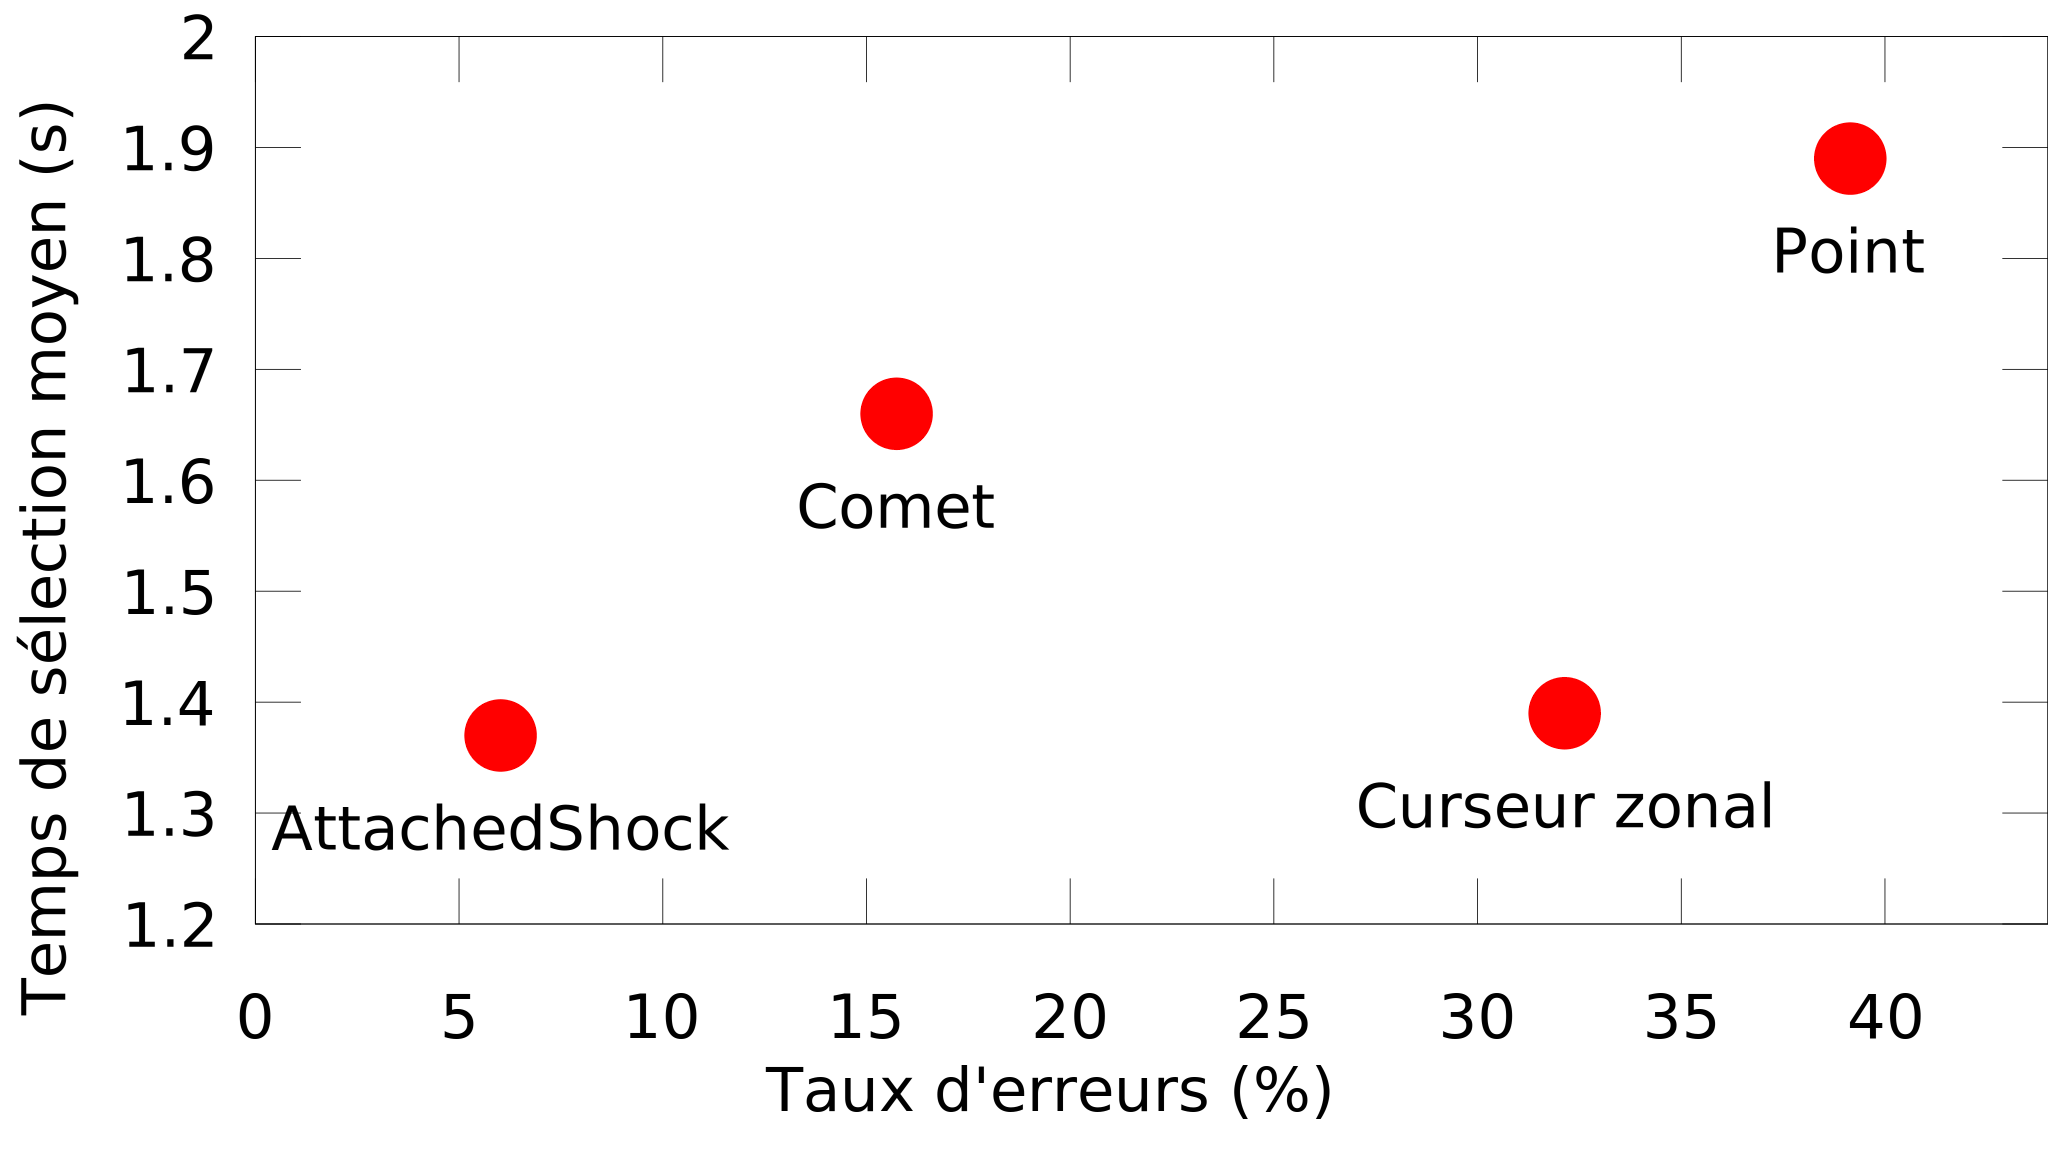
\includegraphics[width=\textwidth]{figures/ch2/asRes}
		\caption[\emph{AttachedShock}, performance]{Présentation des résultats obtenus par les auteurs d'\emph{AttachedShock} au cours de leur évaluation de cette technique. Le taux d'erreurs est en abscisse, et le temps de sélection en ordonnée. Une technique idéale serait donc à l'origine. \emph{AttachedShock} ne fait pas beaucoup mieux qu'un curseur zonal (\emph{Area}) en temps de sélection, mais s'illustre pas un taux d'erreur très bas, et par un temps de sélection moyen qui demeure le meilleur, même s'il est très proche de celui du curseur zonal. Résultats bruts tirés de~\cite{you2012attachedshock}.}
		\label{fig:asRes}
	\end{figure}

	\subsection{Inconvénients}
	\emph{AttachedShock} n'est toutefois pas sans limite. En effet, la densité de cibles testée par les auteurs est très faible, comme le montre la figure~\ref{fig:asDensity}. La technique n'ayant pas été évaluée avec une grande densité de cibles, il est impossible d'affirmer qu'elle fonctionnerait bien dans de telles conditions, mais l'on peut en douter compte tenu du fait qu'elle repose sur la possibilité qu'a l'utilisateur de se « contenter » de mouvements balistiques sans mouvements correctifs, ce qui serait bien difficile avec les nombreux obstacles que de nombreux distracteurs constitueraient.
	
	\begin{figure}[ht]
		\centering
		\includegraphics[width=\textwidth]{figures/ch2/asDensity}
		\caption[\emph{AttachedShock}, densité de cibles]{Captures d'écran du dispositif d'évaluation d'\emph{AttachedShock}. À gauche, l'expérience est menée sur un segment de route rectiligne ; à droite, sur un segment courbe. La sphère rouge est la cible à sélectionner, tandis que les vertes sont des distracteurs. On constate que les distracteurs sont peu nombreux et qu'il est relativement peu probable de « traverser » leur onde de choc en essayant d'atteindre cette de la cible. Crédit: \cite{you2012attachedshock}.}
		\label{fig:asDensity}
	\end{figure}
	
	En outre, dans cette évaluation les cibles sont fixées au sol, et donc ne se déplacent à l'écran qu'à l'horizontale. De fait, leurs ondes de choc se présentent toujours dans la même orientation. Or, dans bien des cas, les cibles peuvent changer de direction en cours de route, ce qui soumettrait logiquement ces ondes de choc à de fréquentes rotations. Dans ces condtions, déclencher un mouvement balistique pour traverser l'onde de choc sans mouvements correctifs serait sans doute beaucoup plus difficile.
	
	Ainsi, si \emph{AttachedShock} présente un intérêt certain pour la sélection de cibles mobiles peu nombreuses (avec peu de distracteurs) se déplaçant à l'horizontale, son efficacité en environnement dense et/ou avec des cibles changeant souvent de direction, \emph{a fortiori} de manière imprévisible, demeure à démontrer. Et compte tenu du fonctionnement de la technique, on peut même s'attendre à une chute significative de son efficacité relative dans ces conditions.

\section{\emph{Hold}}
	\subsection{Principe et avantages}
	Le principe de \emph{Hold}~\cite{hajri2011moving} est très simple : sur déclenchement explicite de la part de l'utilisateur, les cibles deviennent statiques, ce qui facilite considérablement leur sélection puisque cela revient à une simple sélection statique, modélisée par la loi de Fitts. Une particularité de cette technique est que les cibles peuvent être stoppées à tout moment par la pression d'un boutons, et « réactivées » en relâchant le bouton, à volonté. Ce fonctionnement est illustré par la figure~\ref{fig:hold}.
	
	\begin{figure}[ht]
		\centering
		\includegraphics[width=\textwidth]{figures/ch2/hold}
		\caption[La technique \emph{Hold}]{Mode de fonctionnement de la technique \emph{Hold} telle qu'elle fut évaluée dans~\cite{hajri2011moving}. En haut (a,b) le système classique (baptisé \emph{Chase} par Al Hajri \emph{et al.}) : l'utilisateur positionne sa souris sur le flacon rouge pour déclencher la sélection, et doit ensuite cliquer sur le disque noir. Au milieu (c,d) la technique \emph{Hold} ; l'utilisateur doit cliquer sur le flacon bleu pour arrêter la cible, maintenir le bouton pressé, et ne le relâcher que sur le disque noir. En bas (e,f), l'utilisateur doit d'abord positionner sa souris sur le flacon vert, puis peut cliquer librement sur le disque, comme dans le premier cas, ou cliquer sur le flacon pour stopper la cible et relâcher le bouton dessus, comme dans le deuxième cas. Cette technique est appelée \emph{Hybrid} par les auteurs, et a l'avantage d'être plus flexible. En effet, elle permet à un utilisateur de laisser une cible se déplacer avant de la sélectionner, ce qui peut être avantageux si elle se dirige vers le curseur. Crédit : \cite{hajri2011moving}.}
		\label{fig:hold}
	\end{figure}
	
	Cela peut pallier le problème d'occultation inhérent à ce type de technique, qui survient si l'on stoppe le mouvement des objets lorsque la cible visée est occultée par un autre objet --- tout particulièrement dans un contexte 3D. On ajoutera que comme la plupart des techniques portant sur les cibles, \emph{Hold} peut être couplée à une technique de curseur, comme le \emph{Bubble Cursor} ou \emph{DynaSpot}, par exemple.
	
	En pratique, l'évaluation de la technique \emph{Hold} menée par Al Hajri \emph{et al.} montre qu'elle \emph{augmente} le temps de sélection, mais réduit le taux d'erreurs. Les sujets de l'évaluation ont expliqué aux auteurs qu'une fois la cible stoppée, ils ressentaient moins le besoin de se presser pour la sélectionner, vu que la tâche était devenue plus facile. De plus, \emph{Hold} nécessite de cliquer une première fois pour stopper la cible, puis de maintenir le bouton de la souris pressé jusqu'à le relâcher sur la cible, ce qui implique un effort supplémentaire et peut partiellemet expliquer ces résultats. Enfin, le nombre de clics montre que les sujets privilégient la rapidité sans \emph{Hold}, et la précision avec.
	
	On peut néanmoins se demander s'ils auraient été identiques si les utilisateurs avaient été plus encouragés à se dépêcher, par exemple en affichant un chronomètre, ou avec un système de points. Les temps de sélection mesurés en fonction des différents paramètres régissant le mouvement de la cible à sélectionner sont détaillés sur la figure~\ref{fig:holdRes}.
	
	\begin{figure}[H]
		\centering
		\includegraphics[width=\textwidth]{figures/ch2/holdRes}
		\caption[\emph{Hold} --- évaluation]{Résultats de l'évaluation de la technique \emph{Hold}. En haut, les résultats en 1D ; en bas, en 2D. Comme le prédit la loi de Fitts, la difficulté de sélection décroît avec la taille des cibles, et comme d'autres études l'ont montré, elle croît naturellement avec leur vitesse.  Crédit : \cite{hajri2011moving}.}
		\label{fig:holdRes}
	\end{figure}
	
	Toutefois, cette tendance générale s'inverse si l'on s'intéresse aux cibles les plus difficiles à sélectionner, c'est-à-dire celles qui sont rapides, petites, ou \emph{a fortiori} les deux à la fois, comme les résultats présentés sur la figure~\ref{fig:holdSFast} le montrent. C'est assez logique puisque la vitesse en particulier n'a que très peu d'incidence sur la difficulté de sélection avec \emph{Hold}, puisqu'elle s'annule dès que l'utilisateur délenche l'arrêt de la cible. La taille conserve son influence décrite par la loi de Fitts, mais son interaction avec la vitesse disparaît presque totalement.
	
	\begin{figure}[H]
		\centering
		\includegraphics[width=\textwidth]{figures/ch2/holdSFast}
		\caption[\emph{Hold} --- petites cibles rapides]{Résultats de l'évaluation de la technique \emph{Hold} en fonction de la taille et de la vitesse de la cible. En rouge (légende \emph{C}) sont notés les temps de sélection de la technique \emph{Chase}, c'est-à-dire la sélection classique ; en bleu (légende \emph{H}) figurent les temps de sélection de la technique \emph{Hold}. On remarque que dans le cas d'une sélection non assistée, la réduction de la taille de la cible ainsi que l'augmentation de sa vitesse rendent la sélection bien plus difficile. Ces effets sont nettement moins prononcés avec la technique \emph{Hold}, de sorte q'elle fournit de meilleurs résultats que la sélection non assistée pour les cas les plus difficiles. Crédit : \cite{hajri2011moving}.}
		\label{fig:holdSFast}
	\end{figure}
	
	L'on peut supposer, en extrapolant ces résultats, que la technique \emph{Hold} serait encore plus bénéfique sur des cibles encore plus petites ou rapides. Elle devrait logiquement permettre de sélectionner de façon relativement aisée des cibles d'une vitesse originelle quelconque, tandis que sans assistance, des cibles trop rapides peuvent devenir insaisissables.
	
	Il s'avère par ailleurs que la technique \emph{Hybrid} fournit de meilleurs résultats que \emph{Chase} et \emph{Hold}, en 1D comme en 2D. Dans le premier cas, la réduction du temps de sélection est de 12~\%{} par rapport à \emph{Chase} et 20~\%{} par rapport à \emph{Chase}, contre respectivement 13~\%{} et 3~\%{} dans le second cas. Il semble donc que le mode \emph{Hybrid} permette aux utilisateurs de choisir eux-mêmes la stratégie optimale.
	
	La figure~\ref{fig:holdTech} présente les choix de technique faits par les sujets en fonction des paramètres de la cible --- sa taille, sa vitesse, sa direction et l'angle de sa direction.
	
	\begin{figure}[H]
		\centering
		\includegraphics[width=\textwidth]{figures/ch2/holdTech}
		\caption[\emph{Hold} --- choix de la technique]{Les choix de technique faits par les sujets en fonction des paramètres de la cible --- sa taille, sa vitesse, sa direction et l'angle de sa direction. Les résultats de la première ligne de graphiques correspondent aux essais en 1D, et ceux de la seconde, en 2D. On constate que les cibles « faciles » tendent à inciter au choix de \emph{Chase}, que les sujets décrivent comme plus rapide, tandis que les cibles plus difficiles à sélectionner encouragent le choix de \emph{Hold} ou \emph{Hybrid}. La taille et la vitesse sont les paramètres dont l'effet est le plus significatif. Les barres notées \emph{Error} correspondent simplement aux essais ratés, c'est-à-dire ceux pour lesquels le sujet à délenché la sélection hors de la cible. Crédit : \cite{hajri2011moving}.}
		\label{fig:holdTech}
	\end{figure}
	
	La figure~\ref{fig:holdRatio} détaille la répartition entre l'utilisation de \emph{Chase} et \emph{Hold} dans une phase identifiée comme \emph{Hybrid}. Là encore, on constate que la difficultée est corrélée avec une utilisation accrue de la technique \emph{Hold.}
	
	\begin{figure}[H]
		\centering
		\includegraphics[width=\textwidth]{figures/ch2/holdRatio}
		\caption[\emph{Hold} --- répartition \emph{Hold/Chase} en mode \emph{Hybrid}]{épartition entre l'utilisation de \emph{Chase} et \emph{Hold} dans une phase identifiée comme \emph{Hybrid}. L'angle et la direction n'ont pas d'effet significatif mais la vitesse (à mesure qu'elle augmente) et la taille (à mesure qu'elle diminue) sont corrélées avec une utilisation accrue de la technique \emph{Hold}, malgré l'étape supplémentaire qu'elle implique. C'est résultats sont cohérents avec ceux observés hors du mode \emph{Hybrid}. Crédit : \cite{hajri2011moving}.}
		\label{fig:holdRatio}
	\end{figure}
	
	\subsection{Inconvénients}
	Néanmoins et bien qu'il soit atténué, le problème d'occultation demeure. Mais surtout, cette technique impose d'arrêter l'animation ou la simulation à la source des mouvements des cibles, ce qui est inacceptable dans bon nombre d'applications, comme la plupart des jeux vidéo, par exemple.
	
	Pour les simulations moléculaires ou encore le contrôle des espaces aérien, maritime, terrestre, les retransmissions d'événements sportifs, etc., cela implique une perte de connexion avec le réel, qui peut dans certains cas être inacceptable.
	
	Un cas particulier mérite d'être souligné : celui des simulations interactives collaboratives, c'est-à-dire impliquant plusieurs utilisateurs pouvant éventuellement être distants l'un de l'autre, et utiliser des dispositifs différents mais synchronisés. Dans un tel contexte, \emph{Hold} impliquerait soit l'imposition par un utilisateur à tous les autres d'un arrêt de la simulation, soit la désynchronisation des différentes simulations.
	
	Certains jeux vidéo sont également dans ce cas de figure, avec le facteur aggravant qu'ils peuvent impliquer un très grand nombre d'utilisateurs simultanés.
	
\section{\emph{Ray casting}}
	\subsection{Principe et avantages}
	Le \emph{ray casting} est une technique de sélection conceptuellement très simple : un périphérique est utilisé pour lancer un rayon virtuel, généralement le long d'un axe du périphérique. Le rayon peut ensuite croiser un objet, ce qui permet de le sélectionner. Cette technique est parfois appelée \emph{laser gun}~\cite{liang1994jdcad}, et elle est illustrée par la figure~\ref{fig:dCanvas2}.
	
	Elle a plusieurs avantages : elle permet de sélectionner un objet à n'importe quelle distance, sans avoir à se déplacer ; on peut sélectionner un objet très éloigné de la position initiale du curseur sans avoir à faire de grand mouvement, puisqu'il suffit de changer l'orientation du périphérique de pointage, donc d'un simple mouvement de poignet.
	
	Cependant, pour les objets de petite taille apparente, la sélection peut être difficile, car elle requiert une précision angulaire élevée. De plus, si le système de \emph{tracking} qui fournit la position et l'orientation du périphérique de pointage produit un signal bruité, la difficulté de sélection s'en trouve encore accrue. Par conséquent, des techniques dérivées du \emph{ray casting} ont été développées.
	
	Classiquement, on utilisera une technique de cône de sélection, comme par exemple \emph{Spotlight}~\cite{liang1994jdcad}, illustrée par la figure~\ref{fig:spotlight}. Comme le nom l'indique, les techniques de ce typent remplacent le rayon de sélection par un cône dont le sommet est placé sur le périphérique de pointage.
	
	\begin{figure}[H]
		\centering
		\includegraphics[width=\textwidth]{figures/ch2/spotlight}
		\caption[Cône de sélection : \emph{Spotlight}]{Illustration d'une technique de sélection par cône, baptisée \emph{Spotlight}. Les objets qui se trouvent dans le cône sont des candidats à la sélection : quand il y en a plusieurs, le plus proche de l'axe de révolution du cône est choisi ; en cas de proximité égale, le plus proche du périphérique de pointage est choisi. Crédit : \cite{liang1994jdcad}.}
		\label{fig:spotlight}
	\end{figure}
	
	Cela facilite la sélection, puisque les gestes n'ont plus besoin d'être aussi précis, mais peut ajouter de l'ambiguïté si deux objets se trouvent dans le cône de sélection. Le cas échéant, cette ambiguïté peut être levée de plusieurs façon, en fonction de la proximité à l'axe de révolution du cône, en fonction de la distance au périphérique de pointage, ou via une intervention directe de l'utilisateur.
	
	Le choix de l'angle du cône est important : plus il sera grand, plus la sélection sera facile mais potentiellement ambiguë ; plus il sera petit, plus la sélection sera difficile mais spécifique. Le choix de cet angle peut éventuellement être paramétrable, permettant à l'utilisateur de choisir ce qui lui convient le mieux, voire de l'ajuster à la volée en cours d'utilisation. Cet ajustement pourrait également être géré automatiquement par le système interactif, par exemple de façon analogue à ce qui est fait avec des pointeurs classiques dans le \emph{Bubble Cursor}~\cite{grossman2005bubble} ou \emph{DynaSpot}~\cite{chapuis2009dynaspot}.
	
	\subsection{Inconvénients}
	Lorsque l'environnement est particulièrement dense, la sélection par rayon ou cône devient difficile~\cite{kopper2011rapid}, car la précision requise devient très élevée, tant pour l'utilisateur que pour le système de suivi du périphérique de pointage. L'utilisation d'un cône facilite la sélection de petites cibles, mais ajoute un risque d'ambiguïté.
	
	Or, si diverses techniques peuvent aider à lever l'ambiguïté, leur utilisation est d'autant plus difficile que les cibles situées dans le volume du cône sont nombreuses, petites et\ldots{} mobiles. En effet, la mobilité des cibles nécessite d'effectuer des mouvements plus rapides pour les pointer, donc d'exercer plus de force, et de fait, d'être moins précis~\cite{schmidt1979motor}.
	
	Par conséquent, la sélection par rayon ou par cône ne saurait, à elle seule, être une option viable pour sélectionner de nombreuses et petites cibles mobiles, \emph{a fortiori} si elles sont rapides et si leurs mouvements sont imprévisibles.  
	

\section{Sélection en cascade, grossière, puis fine}
	 \subsection{Principe et avantages}
	 Les techniques de cette catégorie divisent la sélection en deux phases (ou plus). Premièrement, une portion de l'espace visuel est sélectionnée. Cette première phase étant grossière, elle n'a pas besoin d'être précise, et peut être très rapide. Par exemple, avec un simple périphérique de pointage, tel qu'une souris, un ratio contrôle/affichage (\emph{control/display, C/D}) très faible peut être utilisé. Le curseur peut ainsi se placer très rapidement sur la zone d'intérêt, mais n'a pas besoin d'être précisément sur la cible pour délencher la deuxième phase : la sélection fine. Dans celle-ci, l'utilisateur sélectionne la cible elle-même, par exemple à l'aide d'un ratio C/D plus élevé.
	 
	 Du point de vue de la loi de Fitts, au cours de la phase grossière, la cible bénéficie d'une largeur accrue (car c'est toute une zone autour de la cible qui est visée) tandis que la phase fine offre une distance réduite, puisque le curseur se trouve déjà près de la cible. Quoiqu'il y ait généralement un certain « coût cognitif » lié au basculement d'une phase à l'autre, les techniques de sélection en cascade peuvent améliorer significativement les performances de sélection, même pour les tâches dont l'indice de difficulté est élevé.[mettre une bonne ref !]
	 
	Un exemple typique de technique de sélection en cascade est la technique \emph{Sphere-casting refined by QUAD-menu
(SQUAD)}~\cite{kopper2011rapid}. 
	 
	La technique du \emph{Disambiguation Canvas} en est un exemple~\cite{debarba2013disambiguation}, illustré par la figure~\ref{fig:dCanvas}. 
		 
	\begin{figure}[H]
		\centering
		\includegraphics[width=\textwidth]{figures/ch2/dCanvas}
		\caption[\emph{Disambiguation Canvas}]{Fonctionnement du \emph{Disambiguation Canvas}, une technique de sélection en cascade. (a) : L'utilisateur pointe vers la région de l'espace où l'objet de son intérêt est situé ; cette présélection se fait par \emph{volume casting}, c'est-à-dire que le périphérique de pointage contrôle un volume de sélection dans l'espace virtuel. (b) : Une fois la présélection faite, une « toile » (\emph{canvas}) de sélection (c'est-à-dire un rectangle partiellement transparent) s'ouvre et les cibles présélectionnées y sont disposées après avoir été agrandies. La toile de sélection correspond à un \emph{mapping} absolu de l'écran tactile d'un périphérique de saisie (un \emph{smartphone}, en l'occurrence, mais cela pourrait être une tablette) ce qui permet à l'utilisateur de sélectionner l'objet désiré avec son pouce. Notez que cette technique est compatible avec les HMD et qu'elle n'affiche pas le petit encadré représentant la main de l'utilisateur en bas à gauche de chaque image ; ces encadrés sont présents ici à des fins purement illustratives. Crédit : \cite{debarba2013disambiguation}.}
		\label{fig:dCanvas}
	\end{figure}
	
	La figure~\ref{fig:dCanvas2} fournit une illustration supplémentaire et peut-être un peu plus claire de cette technique.
	
	\begin{figure}[H]
		\centering
		\includegraphics[width=\textwidth]{figures/ch2/dCanvas2}
		\caption[\emph{Disambiguation Canvas}, bis]{Fonctionnement du \emph{Disambiguation Canvas}. En (a), une photo d'un utilisateur de la technique, équipé d'un HMD et d'un pointeur ; en (b), l'espace virtuel utilisé pour évaluer la technique. Crédit : \cite{debarba2013disambiguation}.}
		\label{fig:dCanvas2}
	\end{figure}
		 
	\subsection{Inconvénients}
	Les techniques de sélection en cascade pouvant prendre des formes très diverses, leurs avantages et inconvénients sont également divers. Néanmoins, elles ont pour principe commun de travailler successivement à différentes échelles, ce qui pourrait être perturbant en environnement immersif, particulièrement lorsque l'on cherche à maintenir une correspondance entre l'espace moteur et l'espace virtuel. Néanmoins, si les gains de performances offerts par la sélection en cascade sont importants, cette perturbation pourrait être une contrepartie acceptable. Notons que la phase grossière ne se fait pas nécessairement avec le même périphérique que la phase fine ; elle peut par exemple se baser sur une estimation de la direction du regard de l'utilisateur, voire se faire automatiquement, par exemple lorsque l'utilisateur focalise son regard sur une zone approximativement constante pendant un certain laps de temps.


% 40% to 70% of gaze displacement is provided by head rotation, while the remaining 60% to 30% result from angular displacement of the eyes in orbit
% http://books.google.fr/books?id=h9FEnj3C7MoC&pg=PA102&lpg=PA102&dq=head+tracking+70%25+of+gaze&source=bl&ots=cp8OJm_G-1&sig=0jsxP3V20VGuxmIvg9CB1sUcyeU&hl=en&sa=X&ei=JFUsU-rVJYam0AW1zYDwAw&redir_esc=y#v=onepage&q&f=false
\section{Suivi de la tête et des yeux}
	\paragraph{}
	Une estimation de la direction du regard de l'utilisateur peut être utilisée soit pour sélectionner directement la cible (ce qui peut nécessiter beaucoup de précision, quand la cible est petite) soit pour sélectionner une zone d'intérêt, dans la phase grossière d'une sélection en cascade. Il y a au moins deux façons d'estimer la direction du regard : la première consiste à capturer les mouvements de la tête de l'utilisateur, et à supposer qu'il regarde droit devant lui. Comme cette hypothèse est généralement fausse, on génère un cone dont le sommet est la tête de l'utilisateur, et dont l'axe de révolution correspond à la direction (estimée) du regard. Or, 40~\%{} à 70~\%{} du déplacement du regard est déterminé par la rotation de la tête, tandis que le reste résulte des mouvements oculaires.[ref bouquin] Si cela s'avère souvent insuffisant pour effectuer une sélection directe, le suivi de tête peut présenter un certain intérêt pour la sélection en cascade.
		
	\paragraph{}
	Pour estimer la direction du regard avec plus de précision, on peut capturer non seulement la position et l'orientation de la tête, mais également l'orientation des yeux. Cette option séduisante présente toutefois quelques difficultés :
	\begin{itemize}
		\item Les performances dépendent de la couleur des yeux ;[ref]
		\item Le suivi des yeux ne fonctionne pas toujours bien en environnement sombre, par exemple dans un CAVE ;[ref]
		\item Les lunettes stéréoscopiques occultent partiellement les yeux pour les \emph{trackers} oculaires, et réduisent la luminosité du blanc des yeux ;[ref]
		\item Le suivi des yeux, souvent combiné à celui de la tête, est plus coûteux que celui de la tête seule ;
		\item Le fait d'utiliser ses yeux pour sélectionner un objet fait du regard une action, rend les utilisateurs conscients de la direction dans laquelle ils regardent, ce qui peut être troublant.
	\end{itemize}

	Par conséquent, l'utilisation de suivi des yeux se montre souvent difficile à mettre en œuvre, quoique les progrès techniques puissent, dans un futur proche, pallier au moins partiellement ces difficultés.
	
\section{\emph{Kinematic Endpoint Prediction}}
	\subsection{Principe et avantages}
	\cite{lank2007endpoint}
	\subsection{Inconvénients}
		
\section{\emph{Speed}}
	\subsection{Principe et avantages}
	\emph{Speed}~\cite{wonner2011speed} est une heuristique de prédiction de cible. Quand l'utilisateur tente de sélectionner une cible, il déplace son curseur vers elle d'une façon que l'on peut séparer en deux phases. Au cours de la première phase, il accélère, tandis qu'il décélère pendant la seconde. C'est dans cette dernière que l'utilisateur est généralement le plus précis. \emph{Speed} base donc sa prédiction de cible sur la phase de décélération. L'heuristique estime la distance que le curseur finira par couvrir à partir de la vitesse du curseur, par ajustement de courbe avec celle d'une fonction quadratique. Quand le curseur a parcouru 85~\%{} de la distance totale estimée, \emph{Speed} utilise la position et la direction courantes du curseur, ainsi que l'estimation de la distance qu'il lui reste à parcourir pour prédire sa destination finale, et par conséquent, la cible visée par l'utilisateur. Cette technique fournit de meilleurs résultats que les précédentes approches de ce type qui ne faisaient pas de distinction entre les phase d'accélération et de décélération.[ref]
			
	\subsection{Inconvénients}
	Cependant, \emph{Speed} part du principe qu'au moment où l'utilisateur décide de sélectionner une cible et commence à déplacer le curseur, il sait quelle cible il veut choisir, où elle se trouve, et donc où placer son curseur. De fait, le mouvement effectué est approximativement rectiligne. Mais si les cibles sont mobiles, alors la trajectoire du curseur ne peut plus être supposée rectiligne. Par conséquent, la précision de \emph{Speed} avec des cibles mobiles est sujette à caution. C'est d'autant plus vrai en environnement dense, car une petite erreur de prédiction a d'autant plus de chances d'aboutir à la sélection d'un distracteur que ceux-ci sont nombreux et près de la cible visée.

		
\section{Hook}
	\paragraph{}
	\emph{Hook} est une heuristique de prédiction de cible. Elle se base sur une évaluation continue de la distance entre le curseur et les cibles potentielles. Celles-ci sont triées par ordre de proximité, et les $NCT$ (\emph{Number of Closest Targets} cibles les plus proches du curseur voient leur score augmenter à chaque boucle de l'heuristique, et augmenter d'autant plus fortement qu'elles sont proches du curseur. Toutes les autres cibles voient leur score diminuer, et diminuer d'autant plus fortement qu'elles sont éloignées du curseur.
		
	\paragraph{}
	La cible potentielle dont le score est le plus élevé est considérée comme celle que l'utilisateur cherche probablement à sélectionner. La sélection peut donc se faire par simple pression d'un bouton, sans contrainte particulière sur la position du curseur au moment où elle est déclenchée.
		
	\paragraph{}
	\emph{Hook} présente plusieurs avantages. Cette technique spécifiquement conçue pour les cibles mobiles fonctionne également pour les cibles statiques. Elle n'ajoute aucun encombrement visuel, ne transforme pas le curseur, ne modifie pas l'apparence des cibles, et n'interrompt pas l'animation ou la simulation en cours. L'évaluation menée par Michael Ortega montre que \emph{Hook} est non seulement plus rapide que le \emph{Bubble Cursor} en 2D comme en 3D, mais permet en plus des taux d'erreur plus faibles. Lorsque les cibles sont rapides, le taux d'erreur peut être moindre d'un facteur supérieur à 4. [ref]

\clearpage

%!TEX root = these.tex

\chapter[Taxinomie des environnements de sélection]{Taxinomie des environnements de sélection de cibles en mouvement}
\minitoc
\label{chap3}
\clearpage

% TODO: Schémas ou tableau pour illustrer le sens de certains critères, genre ciné-discret vs. ciné-continu, etc.
% TODO: Générer des trajectoires avec le modèle VFA à mémoire, pour prouver que ça marche.
% TODO: Idem newtonien ?

\section{Introduction}
	Au cours du premier chapitre de ce manuscrit, nous avons identifié et décrit les besoins de différents domaines d'expertise liés à l'activité de sélection de cibles mobiles. Nous nous sommes en particulier attachés à caractériser la nature des cibles mobiles que l'on rencontre dans ces applications, afin de permettre au lecteur d'apprécier d'une part l'ensemble des difficultés inhérentes aux tâches de sélection dans ces applications, et d'autre part la nécessité d'une assistance à la sélection.
	
	Si nous avons jusqu'ici énuméré et caractérisé ces types de cibles, avec une attention toute particulière à leur contexte applicatif, nous n'avons pas procédé à une classification systématique des cibles selon la nature de leur mouvement, définie selon des critères objectifs et des mesures quantitatives. Or, il nous apparaît que pour réellement comprendre les enjeux et défis liés à la sélection de cibles mobiles, une telle classification est nécessaire.
	
	L'objectif de ce chapitre est donc d'établir une taxinomie des cibles mobiles selon des critères objectifs et, dans la mesure du possible, de permettre une quantification des valeurs auxquelles ils se rapportent. Nous commençons par exposer nos réflexions sur les critères à retenir pour établir cette taxinomie, puis nous confrontons les cibles et leurs environnements à ces critères. Nous présentons ensuite un modèle que nous avons développé pour décrire et générer du mouvement pseudo-aléatoire, régi par des paramètres finement contrôlés. Nous nous appuyons sur ce modèle pour compléter notre taxinomie par des mesures quantitatives et objectives de différents cas applicatifs mobilisant une activité de sélection de cible mobile.	
	
	\section{Critères de discrimination et nature du mouvement}
	Bien qu'une \og simple \fg{} taxinomie des cibles mobiles en fonction de la nature de leur mouvement ait beaucoup d'intérêt, elle ne saurait fournir suffisamment d'informations pour guider la conception de techniques de sélection sans tenir compte de l'\emph{environnement} de sélection. En effet, la cible la plus petite, la plus rapide et la plus imprévisible imaginable est triviale à sélectionner s'il s'agit du seul objet d'intérêt dans l'environnement : il n'y a qu'une sélection possible, donc la technique de sélection optimale --- ou du moins suffisante --- consiste à permettre la sélection de la cible par la simple pression d'un bouton, ou activation d'un quelconque périphérique de saisie.
	
	Dans un tel cas, du point de vue de la théorie de l'information de Shannon~\cite{shannon2001mathematical}, un seul bit d'information est à transmettre de l'utilisateur au système, correspondant à la réponse à la question suivante : \og la cible doit-elle être sélectionnée ? \fg{}. Si la réponse est négative, l'utilisateur ne fait rien et le système non plus ; si elle est positive, une seule action est nécessaire de la part de l'utilisateur, et le système, qui connaît la position de la cible, n'a qu'à la sélectionner sans requérir de précision de la part de l'utilisateur.
	
	Même dans un cas où il y aurait plusieurs objets de ce type, mais en petit nombre, la sélection demeurerait relativement aisée avec une technique telle que le \emph{Bubble Cursor}, analysée au cours du deuxième chapitre. En effet, cette technique illustrée par la figure~\ref{fig:bubble} partage l'espace en plusieurs cellules, selon un diagramme de Voronoï (voir la figure~\ref{fig:voronoi}). De fait, avec par exemple quatre cibles (même très petites, rapides et imprévisibles) l'espace virtuel serait partagé en quatre parties qui, la plupart du temps, seraient très grandes. La loi de Fitts ne s'appliquerait pas directement, car ces zones de sélection seraient mobiles, mais l'on voit bien que la sélection ne serait pas très difficile.
	
	À l'inverse, avec des cibles aussi petites, rapides et imprévisibles, mais extrêmement nombreuses, l'on comprend aisément que l'intérêt du \emph{Bubble Cursor} serait très fortement diminué car les cellules de Voronoï de chaque cible deviendraient fort petites, et pas nécessairement significativement plus grandes que les cibles elles-mêmes.
	
	Il apparaît donc clairement que la difficulté d'une tâche de sélection ne peut être évaluée qu'en tenant compte de l'environnement dans lequel l'objet ciblé est sélectionné. De fait, les besoins et contraintes devant orienter la conception d'une technique d'assistance doivent également en tenir compte. Aussi notre taxinomie tiendra-t-elle compte de l'environnement global, et non seulement de la cible à sélectionner et de la nature de ses mouvements.


	L'établissement de notre taxinomie passe par le choix des critères qui nous permettront d'établir des distinctions entre les types de mouvements des cibles et les environnements de sélection. Dans les sous-sections suivantes, nous allons détailler les critères que nous avons retenus.
	
	\FloatBarrier \subsection{Dimensionnalité}
	Les cibles et leurs environnements se caractérisent notamment par leur nombre de dimensions spatiales. En soi, ce nombre peut varier de un à trois, mais les applications à une seule dimension sont trop rares et trop spécifiques pour entrer dans le cadre de nos travaux. Demeurent donc les objets évoluant dans des espaces 2D/3D. En pratique, la dimensionnalité de l'environnement \og écologique \fg{} des cibles ne correspond pas forcément à la dimensionnalité du dispositif d'affichage ou d'interaction. Les avions, par exemple, évoluent dans un espace tridimensionnel, mais sont généralement affichés sur un plan en 2D sur lequel ils sont projetés ; les périphériques de saisie permettant de les sélectionner sont aussi, généralement, limités à deux degrés de liberté.
	
	\FloatBarrier \subsubsection{Environnements 2D}
	Le contrôle de la circulation routière et des espaces maritimes sont des exemples d'environnements bidimensionnels, si l'on néglige les variations d'altitude sur les routes, les ponts, etc. La surveillance des signaux électromagnétiques entre également dans cette catégorie. Les jeux vidéos tels qu'\emph{Agar.io} (voir figure~\ref{fig:agario}) peuvent aussi présenter des environnements de ce type.
	
	\FloatBarrier \subsubsection{Environnements 3D projetés sur un plan}
	De nombreux types d'objets évoluent dans des environnements 3D mais sont couramment visualisés et sélectionnés à l'aide de systèmes 2D --- par choix, car il est généralement possible d'utiliser des systèmes 3D, et pour certaines applications, c'est occasionnellement le cas. Notons ici les applications pouvant entrer dans la catégorie \og 3D projetée en 2D \fg{}, qu'elles puissent également intégrer la catégorie 3D ou non. Citons donc les simulations moléculaires, le contrôle de l'espace aérien, extra-atmosphérique, maritime quand les sous-marins sont pris en compte, la vidéo-surveillance quand les environnements présentent de forts écarts d'altitude (comme dans un simple bâtiment à plusieurs étages), les retransmissions d'événements sportifs, et enfin la plupart des jeux vidéo dits \og en 3D \fg{} --- à ne pas confondre avec l'immersion en 3D rendue possible par la \emph{stéréoscopie}.
	
	\FloatBarrier \subsubsection{Environnements 3D}
	Parfois, il est possible d'interagir avec un environnement 3D à l'aide d'un dispositif de visualisation immersif et un périphérique de saisie adapté, ayant généralement au moins trois degrés de liberté. C'est occasionnellement le cas des simulations moléculaires et autres applications scientifiques, de certains jeux vidéo, et potentiellement de toutes les applications mentionnées dans la catégorie \og 3D projetée en 2D \fg{}, même si nous n'avons pas connaissance, par exemple, de tels systèmes actuellement utilisés pour le contrôle de l'espace aérien.

	\FloatBarrier \subsection{Autocorrélation}
	Nous considérons ici qu'un mouvement est autocorrélé si un \emph{changement de direction} opéré à l'instant $t$ dépend du \emph{changement} (éventuellement nul) opéré à l'instant $t-1$. Si, au contraire, un changement peut avoir lieu à l'instant $t$ quelle que fût la situation à l'instant précédent, nous appelons ce mouvement \emph{markovien}~\cite{markov1960theory} en admettant qu'il s'agit d'un abus de langage, puisqu'un processus respectant la propriété de Markov est totalement indépendant de l'état du système à l'instant précédent ; or, ici, le vecteur vitesse d'un objet à l'instant $t$ peut dépendre de son orientation à l'instant $t-1$ même si le changement d'orientation n'en dépend pas.
	
	En effet, si ledit changement se fait selon un angle borné (entre -10\textdegree{} et +10\textdegree{}, par exemple) alors l'orientation du vecteur vitesse à l'instant $t$ dépendra de son orientation à $t-1$, puisqu'elle ne pourra différer de celle-ci que de 10\textdegree{}. Tant que le \emph{changement} de direction à l'instant $t$, lui, est bien indépendant du \emph{changement} à l'instant $t-1$, nous admettons cet abus de langage et parlons de mouvement markovien.
	
	Dans le cas contraire, le mouvement est dit autocorrélé. Par exemple, un véhicule effectuant un virage à un instant $t$ est susceptible de maintenir ce virage --- donc le changement de direction correspondant --- à l'instant $t+1$ : le fait que le changement de direction à un instant influence celui de l'instant suivant constitue ce que nous appelons l'autocorrélation. Par commodité, nous appliquons ces termes aux objets autant qu'à leurs mouvements.

	Parmi les objets autocorrélés figurent tous les véhicules que nous avons évoqués au cours du chapitre~\ref{chap1} : les automobiles, navires, aéronefs, engins spatiaux, etc. Au sens strict, tout objet de masse non nulle et macroscopique devrait être autocorrélé, mais nous pouvons considérer que certains peuvent changer de direction de manière si vive et imprévisible qu'ils sont subjectivement markoviens. En règle générale, nous admettons qu'un projectile est autocorrélé, tout en gardant à l'esprit que dans certains cas il peut avoir un comportement subjectivement markovien.
	
	Le cas des jeux vidéo est délicat en ce qu'il s'agit d'un domaine extrêmement vaste dans lequel il est possible de trouver des cibles de toutes natures. Néanmoins, quand ils sont modélisés de manière (subjectivement) réaliste, les objets qui sont autocorrélés dans le monde réel le sont également dans les environnements virtuels des jeux. Enfin, il est possible de rencontrer dans un jeu vidéo n'importe quel type d'objet, réel ou imaginaire. Ceux de la seconde catégorie peuvent être autocorrélés comme markoviens ; il est impossible d'en dresser un inventaire exhaustif, mais disons simplement qu'ils existent --- comme les disques du jeu \emph{Agar.io}, mentionné dans le premier chapitre, qui sont markoviens.

	\FloatBarrier \subsubsection{Uniformité}
	Le mouvement autocorrélé le plus simple est le mouvement uniforme, c'est-à-dire celui pour lequel le vecteur vitesse ne change jamais. Les objets de mouvement uniforme se déplacent donc en ligne droite. Inversement, un mouvement n'est pas uniforme si, à un instant quelconque, la direction ou la norme du vecteur vitesse de l'objet concerné change. Du fait du focus de ce manuscrit sur les cibles mobiles de sélection difficile, nous n'avons pas réellement abordé d'objets aux mouvements uniformes au cours du premier chapitre. Il va sans dire qu'ils existent pourtant. Remarquons néanmoins que si l'on restreint suffisamment la fenêtre temporelle au travers de laquelle on analyse le mouvement d'un objet, l'on peut généralement aboutir à un mouvement localement uniforme.
	
	C'est notamment le cas de véhicules, et particulièrement de ceux qui couvrent de longues distances. Ainsi, les avions et les navires suivent généralement des géodésiques,\footnotemark{} et même une automobile sur une autoroute tend à suivre une trajectoire rectiligne si l'on n'en observe que quelques centaines de mètres. Même un piéton sur un trottoir ou un athlète sur une piste de course peuvent avoir une trajectoire localement uniforme. Les projectiles ayant des trajectoires balistiques, ils ne sont pas de mouvement uniforme, mais peuvent le paraître si ce mouvement est projeté sur un plan horizontal, masquant les variations d'altitude (quoique des variations de vitesse puissent demeurer perceptibles). %Pour être tout à fait exact, un projectile tournant sur lui-même dans l'air (ou un autre fluide) est soumis à l'effet Magnus~\cite{magnus1853ueber, briggs1959effect} et n'a donc pas une trajectoire balistique ; selon l'axe de sa rotation, il peut donc ne pas avoir un mouvement rectiligne une fois sa trajectoire projetée sur un plan horizontal. C'est par exemple le cas d'un ballon de football suite à une \og frappe enroulée \fg{}.

	
	\footnotetext{Une géodésique est une ligne droite sur une surface de géométrie quelconque. Sur une sphère, une géodésique est un \emph{grand cercle}.}
	
	\FloatBarrier \subsubsection{Périodicité}
	Un mouvement sera dit périodique si les changements de direction sont tels que l'objet effectuera une trajectoire qu'il répétera (éventuellement sur une partie seulement) à intervalles réguliers. Plus formellement, un mouvement est périodique s'il admet une période $T$ telle que :	$\forall t,~Pos_{t}~=~Pos_{t+T}$ où $Pos_{t}$ désigne la position de l'objet à l'instant $t$.
	
	Là encore, du fait du focus de ce manuscrit, les objets de mouvement périodique ont peu été abordés au cours du premier chapitre. On les trouve cependant dans certains jeux vidéo, ainsi que dans des applications astronomiques, les objets célestes étant généralement en orbite autour d'un point de l'espace. Les débris spatiaux sont donc des exemples d'objets de mouvement périodique, même s'ils sont susceptibles d'être examinés sur des échelles temporelles trop courtes pour que cette périodicité soit perceptible. Ce n'est cependant pas nécessairement le cas, par exemple si l'on souhaite étudier ces objets dans leur ensemble et sur un temps relativement long, afin d'examiner les dangers qu'ils représentent. La densité de ces objets rend par ailleurs ce cas particulièrement intéressant ; en ceci, nous pouvons le rapprocher de l'étude des anneaux de certaines planètes.\footnotemark{}
	
	\footnotetext{Le cas de Saturne est d'autant plus intéressant qu'en plus d'être nombreux et très riches, ses anneaux ont été étudiés de très près et longuement par la sonde \emph{Cassini}, de sorte que nous avons des informations détaillées dessus.
	
	\url{https://saturn.jpl.nasa.gov/mission/grand-finale/grand-finale-orbit-guide}}
	
	\paragraph{Pseudo-périodicité.}
	Nous appellerons pseudo-périodique un mouvement caractérisé par une trajectoire répétée à intervalles \emph{irréguliers}. Un tel mouvement ne satisfait pas la condition formalisée ci-dessus, mais admet un ensemble de positions limitées à une trajectoire donnée, et revisitées continuellement dans le même ordre --- simplement, à des vitesses pouvant varier.
	
	Les objets de mouvement pseudo-périodique sont très proches (subjectivement) de ceux de mouvement périodique. Ils sont également assez rares dans les applications impliquant une tâche de sélection de cible mobile. Nous pouvons néanmoins citer les véhicules de course sur circuit. Compte tenu des durées des pseudo-périodes concernées, il est cependant peu probable que la pseudo-périodicité soit perceptible par un utilisateur, à moins bien sûr qu'il ne visionne un enregistrement de la course en accéléré. Une telle activité pourrait avoir de l'intérêt, par exemple pour une écurie de Formule~1 cherchant à analyser une course terminée.
	
	\paragraph{Ellipticité et pseudo-ellipticité.}
	Un mouvement (pseudo-)périodique peut être elliptique, voire circulaire. Nous considérons en pratique que les implications pour la tâche de sélection sont presque identiques.
	
	Nous avons déjà examiné le cas des objets célestes dans la catégorie des objets de mouvement périodique, aussi n'est-il pas utile d'y revenir ici, si ce n'est pour préciser qu'ils appartiennent évidemment à la catégorie des objets de mouvement elliptique lorsqu'ils sont en orbite~\cite{kepler1953epitome}. Rares sont les objets non célestes suivant de telles trajectoires, bien que les voitures de course de type NASCAR ou les chevaux de course s'en approchent.
	
	\subsection{Vitesse}
	La vitesse des cibles est un critère essentiel de notre taxinomie, car cette valeur a une très forte influence sur la difficulté de sélection, comme le montrent notamment les résultats empiriques obtenus par Ortega~\cite{ortega2013hook} (voir section~\ref{sub:hook}), ainsi que les travaux de Jagacinksi \emph{et al.}~\cite{jagacinski1980test} (voir section~\ref{sub:fittsMobile}) et ceux d'Al Harji \emph{et al.}~\cite{hajri2011moving} (section~\ref{sub:fittsMobile}). Plus une cible est rapide, plus elle est difficile à sélectionner. Nos propres mesures, sur lesquelles nous reviendrons en détail plus loin, le confirment.
	
	La vitesse \emph{absolue} de la cible n'est pas très importante, seule sa vitesse \emph{relative} (observée à l'écran) compte. Par exemple, la Terre effectue sa rotation autour du Soleil à près de 30~km/s, soit 108~000~km/h. Cette vitesse réelle a pourtant peu de chances d'être un problème dans une application réelle, car une telle application présenterait probablement la Terre à une échelle permettant d'observer son orbite. Or, la Terre mettant environ 365 jours à compléter son orbite, sa vitesse relative serait très faible, donc peu gênante dans une tâche de sélection. À l'inverse, une balle de tennis est comparativement lente ($\approx$~200~km/h), mais étant observée à l'échelle d'un court de tennis (environ 24~m) sa vitesse relative est considérable. De même, un objet dans un jeu vidéo peut se déplacer très lentement, à quelques cm/s seulement ; mais si ce mouvement est observé à l'échelle 1, alors l'objet traversera un écran standard très rapidement.
	
	Or, notre taxinomie vise à classifier les cibles et leurs environnements selon les difficultés de sélection qu'ils présentent et non selon leurs caractéristiques absolues ; de fait, nous nous intéressons aux vitesses relatives des objets examinés. Ce choix est lourd de conséquences car la vitesse relative d'un objet d'une vitesse réelle donnée dépend des conditions dans lesquelles il est affiché, en particulier de l'échelle relative à la taille du dispositif d'affichage, et de ladite taille. Elle dépend également, pour tout ce qui n'est pas joué à vitesse réelle, de la vitesse choisie pour l'animation ou la simulation.
	
	La taxinomie que nous proposons implique de faire des choix. La vitesse des objets est un critère de discrimination essentiel, qui impose de discrétiser un espace continu. Dans un souci de simplicité, nous avons choisi de le réduire à deux catégories : les objets rapides et les objets lents. Ce choix est quelque peu arbitraire et subjectif, mais nécessaire, et nous semble d'autant plus justifié que c'est justement l'impression subjective des utilisateurs face à un certain type de mouvement qui nous intéresse, car nous faisons l'hypothèse (sur laquelle nous reviendrons) que cette impression subjective est corrélée aux performances de sélection.
	
	\FloatBarrier \subsubsection{Variabilité de la vitesse}
	Il serait pratique de pouvoir résumer la vitesse à une variable scalaire, mais ce n'est malheureusement pas toujours possible. En effet, dans les applications identifiées le long du chapitre~\ref{chap1}, la vitesse des objets est généralement variable. L'on ne saurait donc la résumer par un simple nombre. Dans l'idéal, il serait bon de connaître toutes les vitesses atteintes par les objets de la scène, avec leurs fréquences d'occurrence ; cela nous permettrait d'en dresser un histogramme. Connaissant toutes ces valeurs, l'on pourrait les représenter de façon plus concise par une moyenne et un écart-type ; il serait sans doute opportun d'ajouter à cette représentation la vitesse maximale possible, afin de pouvoir caractériser le cas (potentiellement) le plus difficile. Pour certaines applications, il sera difficile voire impossible d'avoir des informations aussi précises. Dans ce cas, nous devrons nous contenter d'une estimation aussi précise que possible des valeurs sus-citées, par exemple d'une vitesse \og typique \fg{} et d'une vitesse maximale.
		
	\FloatBarrier \subsubsection{Objets lents, objets rapides}
	Le mode de visualisation détermine souvent la vitesse apparente des objets. À grande échelle, les véchicules paraissent lents. En règle générale, les piétons observés dans des enregistrements de mouvements de foule sont assez lents, exception faite des émeutes, où les mouvements se font plus vifs. À petite échelle, tout type de véhicule peut paraître rapide. La lenteur d'une cible mobile rend sa sélection plus aisée, mais des objets lents peuvent néanmoins être petits, distants, présents dans des environnements très denses, (partiellement) occultés, et caractérisés par des mouvements imprévisibles. Il serait donc imprudent de considérer qu'ils sont \og faciles \fg{} à sélectionner sur la seule base de leur lenteur.
	
	Dans la grande majorité des cas, les particules des simulations moléculaires sont (très) rapides à l'écran. Les athlètes peuvent également être assez rapides (les skieurs ou patineurs de vitesse, par exemple) mais c'est encore plus vrai des projectiles qu'ils utilisent. Enfin, les jeux vidéo regorgent d'objets de vitesses extrêmement variées, et il n'y a pas de borne maximale pratique à la vitesse des objets vidéoludiques.
	
	\FloatBarrier \subsubsection{Accélération}
	Au-delà des valeurs typiques ou maximales de la vitesse, il peut être judicieux d'examiner dans quelle mesure la vitesse varie en un court laps de temps, c'est-à-dire la façon dont les objets accélèrent. En effet, un objet se déplaçant lentement peut paraître aisé à sélectionner, mais s'avérer difficile s'il accélère brutalement, surtout au moment où l'utilisateur effectue son mouvement de sélection. Là encore, l'idéal serait d'avoir un histogramme, une moyenne, un écart-type et un maximum. L'on devra souvent se contenter d'une valeur typique et d'un maximum estimés. Ce sera généralement suffisant pour répondre à la question primordiale concernant l'accélération : \og la cible est-elle susceptible d'accélérer brusquement ? \fg{}. Les objets accélèrent généralement d'autant plus facilement qu'ils sont légers, et les atomes peuvent le faire brusquement, y compris dans les simulations de dynamique moléculaire.

	Les objets de vitesse \emph{strictement} constante sont rares, mais pas inexistants. La table~\ref{tab:dotamoves}, par exemple, fournit les vitesses des personnages les plus vifs d'un jeu vidéo, et ces vitesses sont constantes (sauf effets magiques ou autres). Certains des objets de mouvement circulaire ont également une vitesse constante. Cependant, si l'on assouplit quelque peu notre critère pour inclure, d'une part, les objets de vitesse \emph{approximativement} constante et, d'autre part, les objets de vitesse constante sur une partie (significative) de leur trajectoire, alors nous pouvons ajouter de nombreux véhicules (quand une vitesse de croisière est maintenue pendant un temps assez long), les objets célestes (pour peu que l'excentricité de leur orbite ne soit pas trop élevée --- car de celle-ci dépendent les variations de vitesse), les piétons en marche, ou les athlètes pendant une course d'endurance.
	
	Comme la vitesse, l'accélération est une quantité réelle. De fait, son utilisation comme critère de discrimination implique de la discrétiser. Distinguons simplement les objets dont l'accélération est négligeable de ceux dont elle est clairement perceptible ou particulièrement élevée. Nous définissons ici l'accélération comme la dérivée de la \emph{vitesse} (la valeur scalaire représentant la norme de la vélocité) et non de la \emph{vélocité} (qui est une valeur vectorielle). Nous partons donc du principe qu'un objet changeant brusquement de direction tout en maintenant une vitesse constante a une \og accélération \fg{} nulle, même si sa vélocité change brusquement, par exemple en passant de $\vec{v}_{t} = (0,1)$ à $\vec{v}_{t+1} = (1,0)$, où le vecteur vélocité est inversé mais la vitesse demeure constante et vaut 1.
	
	Beaucoup d'objets vidéoludiques peuvent accélérer de façon plus ou moins vive, selon les circonstances --- c'est même le cas des personnages de jeux vidéo cités plus haut, qui peuvent passer d'une vitesse nulle à leur vitesse maximale de façon presque instantanée.\footnotemark{} Les véhicules accélèrent aussi, dans des mesures diverses : bien en dessous d'un $g$ pour une automobile ordinaire ou un gros navire, environ $1~g$ pour un avion de chasse (ou Usain Bolt\footnotemark{}), ou plusieurs dizaines de $g$ pour certains missiles.\footnotemark{}

	\addtocounter{footnote}{-2}
	\footnotetext{Dans bien des jeux, cette accélération se fait en l'espace d'une \emph{frame}, c'est-à-dire (grossièrement) d'une itération de la boucle de jeu, soit un peu moins de 17~ms dans la plupart des cas.}
	\addtocounter{footnote}{1}
	\footnotetext{\url{http://io9.gizmodo.com/the-physics-of-usain-bolts-world-record-100-meter-dash-924744818}}
	\addtocounter{footnote}{1}
	\footnotetext{\url{http://www.designation-systems.net/dusrm/app4/sprint.html}}
	
	Les objets nanoscopiques tels que les atomes peuvent accélérer si vivement qu'une tentative de quantifier cette accélération en $g$ n'aurait que peu de sens, surtout du point de vue d'une interface homme-machine nécessairement limitée par la fréquence de rafraîchissement de son dispositif d'affichage, située entre 60~Hz et 240~Hz en général,\footnotemark{} voire 1~kHz sur le canal haptique~\cite{perret2013interactive}. Quand bien même cette limite technique n'existerait pas, il est douteux qu'un humain puisse percevoir une différence à l'œil nu entre les quelque 10~000~$g$ d'un coup de squille (ou crevette-mante)~\cite{patek2004biomechanics} et les 100~000~$g$ d'une morsure de fourmi \emph{Odontomachus}~\cite{patek2006multifunctionality}. Observons simplement que ces objets peuvent accélérer très vivement.
	
	\footnotetext{\url{https://www.blurbusters.com/faq/120hz-monitors}}
	   
	\FloatBarrier \subsection{Fréquence des changements de direction}
	Pour les objets macroscopiques réels, la direction est généralement soit constante, soit en changement continu. Par exemple, une automobile peut rouler droit devant elle pendant un certain temps, puis, pendant une durée généralement plus courte, suivre une trajectoire courbe caractérisée par une rotation continue de son vecteur vitesse. Dans ce cas, il est difficile de parler de \emph{fréquence} des changements de direction, comme s'ils étaient des événements ponctuels et discrets, à moins de considérer cette fréquence comme étant soit nulle (car il n'y a jamais de changement brusque), soit infinie (car il y a un changement constant). Dans les deux cas, ce n'est guère utile pour caractériser le mouvement.
	
	Parfois, cependant, il peut être pertinent de considérer un changement de direction relativement court et rapide comme un événement se produisant à un instant bien défini. Pour reprendre l'exemple de l'automobile, il est clair que cette approximation posera généralement des problèmes pour les trajets à grande vitesse, par exemple sur les autoroutes --- les courbes y sont très douces et, de fait, les changements de direction sont lents et continus. À plus basse vitesse, cependant, et notamment pendant la circulation urbaine, il est possible d'effectuer un virage à (plus de) 90\textdegree{} sur un temps beaucoup plus court. Dans ces conditions, assimiler ce virage à une rotation instantanée du vecteur vitesse est plus raisonnable, compte tenu de la perception subjective d'un utilisateur.
	
	Les objets nanoscopiques, du moins tels qu'ils sont généralement simulés, tendant à changer de direction de manière abrupte, et la notion de fréquence de changement de direction a généralement du sens. La fréquence qui nous intéresse ici est celle affichée à un utilisateur, car nous ne nous préoccupons que de ce qu'un utilisateur perçoit et de la mesure dans laquelle cela influe sur ses performances de sélection. Et dans les simulations moléculaires, par exemple, cette fréquence dépend de la vitesse à laquelle on joue une animation, ou affiche une simulation, comme pour la vitesse des cibles.
	
	Les objets virtuels tels que ceux rencontrés dans les jeux vidéo ne sont soumis à aucune contrainte physique, et leurs directions peuvent changer de manière instantanée ou continue, selon les choix des développeurs ; dans certains cas, cette notion de fréquence aura donc du sens, et dans d'autres, non.
	
	\subsubsection{Cinématique discrète ou continue}
	\label{sub:kinematicTypes}
	Afin de les différencier, nous disons que les objets dont les changements de direction sont instantanés sont de cinématique discrète, tandis que les autres sont de cinématique continue. Par souci de concision, nous appelons les premiers ciné-discrets et les seconds ciné-continus. Dans la plupart des cas, les objets markoviens sont ciné-discrets et les objets autocorrélés sont ciné-continus, de telle sorte que ces termes sont presque interchangeables. Ce n'est toutefois pas systématiquement le cas, d'où l'utilisation de ces quatre termes.
	
	\subsubsection{Variabilité}
	Comme pour la vitesse, la fréquence des changements de direction d'une cible n'est pas nécessairement constante. Il n'est pas évident de déterminer comment comptabiliser les différentes fréquences au cours de la trajectoire d'un objet. Nous proposons de compter les périodes $T_{i}$ entre chaque changement de direction, et de calculer l'ensemble des $F_{i} = 1/T_{i}$. De même que pour la vitesse, on tâchera donc d'obtenir un histogramme des valeurs, une moyenne, un écart-type, et un maximum.
	
	Dans l'impossibilité de le faire, nous opterons pour une estimation des valeurs \og typique \fg{} et maximale. Illustrons simplement ce propos par l'exemple d'une automobile : sur autoroute, sa fréquence de changements de direction sera presque nulle ; en ville, elle sera bien plus élevée.
	
	\FloatBarrier \subsubsection{Objets ciné-continus, ciné-discrets}
	Cette catégorie contient la plupart des objets autocorrélés : véhicules, projectiles, objets célestes, etc. Certains objets vidéoludiques sont également (perçus comme) ciné-continus et, pour un petit nombre d'entre eux, peuvent être markoviens, du moins dans certains cas. Le jeu \emph{Agar.io}, cité dans le chapitre~\ref{chap1}, en est un exemple.
	
	Les objets markoviens sont généralement ciné-discrets. Nous trouvons donc dans cette catégorie les atomes des simulations moléculaires, divers objets de jeux vidéo\ldots{} Mais précisons que bien qu'ils soient, au sens strict, incapables de changer de direction \emph{instantanément}, certains objets paraissent subjectivement le faire de façon suffisamment soudaine pour que nous les considérions comme ciné-discrets.
	
	C'est par exemple le cas des êtres humains en mouvement, et \emph{a fortiori} de plus petits animaux plus vifs, dont l'exemple le plus emblématique est peut-être la mouche, connue pour ses trajectoires saccadées, avec des changements de direction d'environ 90\textdegree{} en moins de 100~ms~\cite{tammero2002influence, collett1975visual, wagner1986flight, schilstra1999blowfly} --- nous reviendrons plus loin sur cette classe de mouvement.
	
	\FloatBarrier \subsubsection{Objets changeant de direction à basse fréquence}
	Posons comme définition que pour un objet ciné-discret, sa fréquence de changements de direction est \og basse \fg{} si elle est inférieure ou égale à 1~Hz. Si l'objet est ciné-continu, nous dirons que sa fréquence est basse (par abus de langage) si, sur la durée de son mouvement, la proportion du temps qu'il passe à changer de direction est faible.
	
	Ce critère est arbitraire, voire subjectif, mais c'est inévitable pour dresser une taxinomie pertinente. Classons dans cette catégorie les véhicules (ou les missiles) \og en croisière \fg{} : avions de ligne, gros navires, automobiles sur autoroute, etc. En effet, une automobile, par exemple, satisfait généralement les critères définissant cette catégorie, exception faite des déplacements particulièrement rapides ou irréguliers, par exemple sur des routes sinueuses ou dans des environnements urbains exigus.
	
	Les piétons et les plus petits véhicules peuvent entrer dans cette catégorie, selon la nature de leurs déplacements. Les athlètes n'en font partie que pour certaines disciplines bien précises --- courses d'endurance ou cyclisme dans certains cas, notamment. Comme d'habitude avec les jeux vidéo, certains objets qui les peuplent font partie de cette catégorie, et d'autres non.
	
	\subsubsection{Objets changeant de direction à haute fréquence}	
	Les objets de haute fréquence par excellence sont les atomes des simulations moléculaires. Ils peuvent changer de direction à chaque itération de la simulation, ce qui peut aisément dépasser 60~Hz.
	
	Parmi les objets ciné-continus, citons les petits bateaux, les automobiles et surtout les aéronefs militaires, particulièrement au combat : dans ces situations, ils tendent à changer de direction en permanence, de manière imprévisible. Les missiles peuvent présenter des caractéristiques similaires. Même un piéton se frayant un chemin à travers une foule peut avoir des changements de direction très fréquents\ldots{} en particulier s'il cherche à échapper aux forces de l'ordre le poursuivant ou le surveillant. Dans la plupart des cas, les athlètes ont des changements de direction fréquents, surtout dans les sports \og vifs \fg{}. Les projectiles, notamment sportifs, ont des trajectoires balistiques ou plus irrégulières (rebonds, effets\ldots{}) ; ils sont donc dans cette catégorie également. Enfin, les jeux vidéo regorgent d'objets de ce type, qu'il faut souvent viser et détruire.
	
	\subsection{Amplitude des changements de direction}
	Les changements de direction doivent aussi être examinés selon leur amplitude : quand une cible change de direction, son vecteur vitesse subit une rotation. C'est l'angle de cette rotation que nous appelons \emph{l'amplitude} du changement de direction. Pour une fréquence donnée, si cette valeur est faible, la direction de l'objet changera peu et sa trajectoire sera relativement \og lisse \fg{}, comme sur la plupart des exemples de la figure~\ref{fig:motion1530}, sauf ceux dont la fréquence est élevée ($\geq$~16~Hz). Si elle est élevée, en revanche, la trajectoire sera très \og irrégulière \fg{}, comme on l'observe notamment sur la figure~\ref{fig:motion165180}, même à basse fréquence (les amplitudes données dans ces figures sont des valeurs maximales --- nous y reviendrons).
	
	\subsubsection{Nature discrète ou continue}
	Comme mentionné plus haut, un changement de direction peut être considéré comme un événement instantané et discret, ou continu. Dans le premier cas, il aura une valeur en degrés : l'angle entre la direction avant et après le changement ; dans le second, il aura une valeur en degrés/seconde : le taux de changement de direction en fonction du temps. En règle générale, les objets ciné-discrets peuvent avoir des amplitudes de changements de direction très élevées, tandis que les objets ciné-continus tendent à avoir des taux de changement de direction assez faibles, et ce d'autant plus qu'ils sont massifs. Pour un gros navire, par exemple, le rayon de giration minimal peut dépasser les 3~km.\footnotemark{}
	
	\footnotetext{Le rayon de giration est le rayon du cercle parcouru par un objet en mouvement circulaire uniforme. Pour l'exemple cité :
	\url{http://www.container-transportation.com/world-largest-ship.html}}
	
	\subsubsection{Variabilité}
	La variabilité est peut-être plus importante encore que pour la vitesse d'une cible ou la fréquence de ses changements de direction. En effet, rares sont les cibles dont les changements de direction se font toujours selon le même angle, à l'exception des cibles aux mouvements circulaires. Après discrétisation en cas de mouvement continu, un histogramme de ces valeurs peut être retenu, ainsi qu'une moyenne, un écart-type, et un maximum. À défaut, une moyenne et un maximum estimés suffiront.
	
	\subsubsection{Changements de faible amplitude}
	Les objets ciné-discrets dont les changements de direction sont de faible amplitude sont rares, sauf dans les jeux vidéo. Les objets ciné-continus, en revanche, ont souvent des changements de direction de faible amplitude : citons les véhicules lourds, les projectiles, les piétons ou même certains athlètes, comme les skieurs\ldots{} Les jeux vidéo en contiennent également beaucoup.
		
	\subsubsection{Changements de forte amplitude}
	Les objets ciné-discrets dont les changements de direction sont de forte amplitude incluent en premier lieu les atomes des simulations moléculaires, qui peuvent changer de direction de manière totalement libre à chaque itération de la simulation. On trouvera également de tels objets dans les jeux vidéo, dans des jeux comme le billard électrique (ou \emph{flipper}) mais surtout le billard (\emph{pool}, \emph{snooker}\ldots{}). Parmi les objets ciné-continus, l'on peut trouver la plupart des petits véhicules, mais aussi les piétons, les athlètes de nombreuses disciplines; et bien sûr des objets vidéoludiques.


	\subsection{Densité de l'environnement}
	Une caractérisation précise d'un environnement de sélection doit inclure une estimation de sa densité. Celle-ci peut se calculer en nombre d'objets pouvant être sélectionnés par unité de surface (pour un espace en 2D, ou un plan sur lequel un espace 3D serait projeté) ou par unité de volume. L'espace des densités est continu mais, pour les besoins de la taxinomie, on peut le discrétiser en un nombre fini de niveaux, définis par des intervalles de densité mutuellement disjoints. Plutôt que le nombre d'objet, il est également possible de considérer leur volume total, afin d'obtenir une valeur comprise entre 0 et 1.
	
	\FloatBarrier \subsubsection{Occultation}
	Le niveau d'occultation visuelle d'un environnement est également crucial. Il dépend fortement de la densité de l'environnement, mais n'y est pas équivalent. En effet, pour une densité donnée, le niveau d'occultation peut être très élevé si les cibles sont très grosses et opaques ; si, en revanche, elles sont relativement petites, voire semi-transparentes, l'occultation peut être assez faible. Par exemple, la même molécule est représentée sur la figure~\ref{fig:4awn_VdW} et sur la figure~\ref{fig:4awn_points}, mais le niveau d'occultation est bien plus élevé dans le premier cas que dans le second. En outre, la \og taille \fg{} des cibles ne peut pas forcément s'exprimer de façon adéquate avec une valeur scalaire. En effet, si la taille d'une cible sphérique est correctement exprimée par son seul rayon, il en va autrement d'un objet d'une forme quelconque, et \emph{a fortiori} complexe.
	
	Pour ces raisons et d'autres, l'estimation du niveau d'occultation est difficile, et mériterait sans doute une étude très poussée. Peut-être serait-il opportun de la quantifier par une estimation de la probabilité qu'un objet quelconque soit totalement occulté, ou suffisamment occulté pour qu'un utilisateur manque de le remarquer avec une certaine probabilité donnée. Par souci de simplicité, nous devons ici nous contenter d'une estimation subjective de l'occultation, que nous exprimons par un ensemble fini de niveaux. Quoi qu'il en soit, attendu qu'il est généralement nécessaire de voir ou d'avoir vu un objet pour le sélectionner, il s'agit d'un critère important.
	
	L'utilisation de la densité d'un environnement et du niveau l'occultation implique là encore de discrétiser l'espace d'une variable réelle. Nous choisissons de définir la limite entre un environnement de faible densité et un environnement de forte densité comme le nombre de cibles mobiles à partir duquel il devient difficile voire impossible pour l'utilisateur de les compter. Notez que le mouvement des cibles rend le comptage nettement plus difficile. Précisons qu'une application donnée peut présenter des niveaux de densité et d'occultation parfois très variables, donc entrer dans les deux catégories.
	
	\subsubsection{Faibles densité et occultation}
	Selon les cas, les environnements urbains, routiers, maritimes, aériens, ou extra-atmosphériques peuvent présenter une faible densité, donc peu ou pas d'occultation. De nombreux sports entrent également dans cette catégorie, ainsi que des jeux vidéo. Cependant, un environnement de faible densité peut présenter un niveau d'occultation élevé, selon le point de vue. Cela peut par exemple être le cas d'une retransmission d'événement sportif filmé depuis le côté, comme sur la figure~\ref{fig:basketball}.
	
	\subsubsection{Fortes densité et occultation}
	Les simulations moléculaires sont souvent très denses, avec beaucoup d'occultation. C'est parfois également le cas de la vidéosurveillance, du contrôle des espaces fluides ou des signaux électromagnétiques, voire de la circulation routière. Certains sports et jeux vidéos sont aussi concernés. Attention toutefois : même une foule extrêmement dense, observée depuis le ciel, directement au-dessus, pourrait avoir un taux d'occultation nul.
	
\section{Modèle de génération de mouvement}
	Afin d'étudier rigoureusement la sélection de cibles mobiles en fonction de la nature du mouvement, il est nécessaire de pouvoir générer différents types de mouvements avec le plus petit nombre de paramètres possible. Dans l'idéal, le modèle choisi pour la génération de mouvement devrait être capable d'en générer une très grande variété. Les objectifs de variété et d'économie de paramètres étant contradictoires, un compromis doit être atteint. Dans le but d'obtenir un modèle relativement simple et facilement exploitable, nous avons choisi de nous limiter aux mouvements markoviens ; ce choix fut également motivé par le fait que ces mouvements sont intrinsèquement moins prévisibles et, par conséquent, plus difficiles à anticiper --- ils rendent de fait la sélection plus difficile.
	
	\FloatBarrier \subsection{Trois paramètres pour le mouvement synthétique}
	Nous avons opté pour un modèle (baptisé VFA) limité à trois paramètres pour définir le mouvement d'un objet de vecteur vitesse $\vec{dir}$ (indiquant sa direction par son orientation, et sa vitesse par sa norme) :
	\begin{enumerate}
		\item La vitesse $V$ à laquelle l'objet se déplace ;
		\item La fréquence $F$ des changements de $\vec{dir}$ ;
		\item L'angle maximal $A$ de ces changements de direction : à chaque période $T = \frac{1}{F}$, $\vec{dir}$ subit une rotation d'un angle $\alpha$ choisi aléatoirement et échantillonné uniformément dans l'intervalle $[-A, +A]$.
	\end{enumerate}
	
	Ces paramètres sont analogues à ceux choisis pour évaluer \emph{Comet}~\cite{hasan2011comet} et, dans une certaine mesure, \emph{Hook}~\cite{ortega2013hook}.
	
	\subsubsection{Gestion de la dimensionnalité et de la densité}
	L'objectif de ce modèle est de caractériser la nature des mouvements de cibles, ou de les générer. Il s'applique aux cibles elles-mêmes et non aux environnements de sélection dans leur ensemble. C'est pourquoi la dimensionnalité et la densité ne sont pas exprimées explicitement par ce modèle. Il s'en accommode néanmoins, puisqu'il est tout à fait possible d'animer une cible 2D ou 3D avec ces paramètres, et d'obtenir la densité voulue. En effet, la dimensionnalité n'implique qu'une différence : en 2D, l'angle $\alpha$ choisi aléatoirement à chaque période suffit à déterminer la nouvelle direction de la cible. En 3D, pour un angle $\alpha$ donné, les nouvelles directions possibles sont infinies, et réparties sur la surface d'un cône d'angle $\alpha$. Il suffit donc de choisir aléatoirement une direction sur ce cône.
	
	La densité, elle, est indépendante des paramètres de ce modèle : elle ne dépend que de la taille de l'environnement de sélection et de l'ensemble des cibles. Il suffit donc d'ajuster ces paramètres ; le modèle que nous proposons permet d'animer les cibles, indépendamment de la densité voulue.
	
	\subsubsection{Omission de l'autocorrélation}
	Nous avons délibérément choisi de ne pas retenir, dans cette version du modèle, de paramètre lié à l'autocorrélation. Ce choix est en partie motivé par l'absence d'autocorrélation des cibles dans les trajectoires de dynamique moléculaire, mais surtout par le fait qu'en choisissant les paramètres astucieusement, le modèle VFA peut simuler du mouvement autocorrélé de manière relativement convaincante, comme nous le montrons dans la section~\ref{sub:pseudoAutoCorr}.
	
	Par ailleurs, nous proposons deux extensions possibles de notre modèle VFA visant à gérer explicitement et correctement l'autocorrélation, pour les cas où la pseudo-autocorrélation permise par le modèle VFA de base ne serait pas suffisante. Ces propositions sont détaillées dans la section~\ref{sub:vfaAutoCorr}.
	
	\FloatBarrier \subsection{Examen des trajectoires obtenues}
	Des exemples de trajectoires obtenues avec ce modèle sont fournis dans les figures~\ref{fig:motion1530} avec $A=15$ et 30, \ref{fig:motion4560} avec $A=45$ et 60, \ref{fig:motion7590} avec $A=75$ et 90, \ref{fig:motion105120} avec $A=105$ et 120, \ref{fig:motion135150} avec $A=135$ et 150, et~\ref{fig:motion165180} avec $A=165$ et 180. Dans tous les cas, $S=2,19$, avec $F \in \{1,4,8,16,32,60\}$, et le mouvement généré dure 20 secondes. A est exprimé en degrés d'angle, F en Hz, et S en cm/s. Naturellement, si la vitesse était plus élevée, les trajectoires seraient plus \og dilatées \fg{}, et plus \og comprimées \fg{} si elle était plus faible (voir la figure~\ref{fig:spEffect}). De plus, si $A=0$ ou $F=0$, alors il n'y a aucun changement de direction, et le mouvement est uniforme (rectiligne). Si nous avons échantillonné tout l'espace des valeurs de $A$ possibles --- de 0 à 180\textdegree{} --- nous nous sommes limités à 60~Hz pour la fréquence, d'une part parce qu'il devient difficile de percevoir une différence marquée dès qu'elle atteint une trentaine de hertz, et d'autre part parce que la plupart des dispositifs d'affichage du commerce sont limités à 60~Hz.	
	
	\newcommand{\subImgWarea}{0.42\textwidth}
	\begin{figure}[htb]
		\begin{subfigure}[t]{\subImgWmo}
			\centering
			\includegraphics[width=\textwidth]{figures/ch3/synTraj_219_15_1}
			\caption[$A = 15$, $F=1$]{$A = 15$, $F=1$}
			\label{fig:synTraj_219_15_1}
		\end{subfigure}
		~
		\begin{subfigure}[t]{\subImgWmo}
			\centering
			\includegraphics[width=\textwidth]{figures/ch3/synTraj_219_15_4}
			\caption[$A = 15$, $F=4$]{$A = 15$, $F=4$}
			\label{fig:synTraj_219_15_4}
		\end{subfigure}
		~
		\begin{subfigure}[t]{\subImgWmo}
			\centering
			\includegraphics[width=\textwidth]{figures/ch3/synTraj_219_15_8}
			\caption[$A = 15$, $F=8$]{$A = 15$, $F=8$}
			\label{fig:synTraj_219_15_8}
		\end{subfigure}
		~
		\begin{subfigure}[t]{\subImgWmo}
			\centering
			\includegraphics[width=\textwidth]{figures/ch3/synTraj_219_15_16}
			\caption[$A = 15$, $F=16$]{$A = 15$, $F=16$}
			\label{fig:synTraj_219_15_16}
		\end{subfigure}
		~
		\begin{subfigure}[t]{\subImgWmo}
			\centering
			\includegraphics[width=\textwidth]{figures/ch3/synTraj_219_15_32}
			\caption[$A = 15$, $F=32$]{$A = 15$, $F=32$}
			\label{fig:synTraj_219_15_32}
		\end{subfigure}
		~
		\begin{subfigure}[t]{\subImgWmo}
			\centering
			\includegraphics[width=\textwidth]{figures/ch3/synTraj_219_15_60}
			\caption[$A = 15$, $F=60$]{$A = 15$, $F=60$}
			\label{fig:synTraj_219_15_60}
		\end{subfigure}
		~
		\begin{subfigure}[t]{\subImgWmo}
			\centering
			\includegraphics[width=\textwidth]{figures/ch3/synTraj_219_30_1}
			\caption[$A = 30$, $F=1$]{$A = 30$, $F=1$}
			\label{fig:synTraj_219_30_1}
		\end{subfigure}
		~
		\begin{subfigure}[t]{\subImgWmo}
			\centering
			\includegraphics[width=\textwidth]{figures/ch3/synTraj_219_30_4}
			\caption[$A = 30$, $F=4$]{$A = 30$, $F=4$}
			\label{fig:synTraj_219_30_4}
		\end{subfigure}
		~
		\begin{subfigure}[t]{\subImgWmo}
			\centering
			\includegraphics[width=\textwidth]{figures/ch3/synTraj_219_30_8}
			\caption[$A = 30$, $F=8$]{$A = 30$, $F=8$}
			\label{fig:synTraj_219_30_8}
		\end{subfigure}
		~
		\begin{subfigure}[t]{\subImgWmo}
			\centering
			\includegraphics[width=\textwidth]{figures/ch3/synTraj_219_30_16}
			\caption[$A = 30$, $F=16$]{$A = 30$, $F=16$}
			\label{fig:synTraj_219_30_16}
		\end{subfigure}
		~
		\begin{subfigure}[t]{\subImgWmo}
			\centering
			\includegraphics[width=\textwidth]{figures/ch3/synTraj_219_30_32}
			\caption[$A = 30$, $F=32$]{$A = 30$, $F=32$}
			\label{fig:synTraj_219_30_32}
		\end{subfigure}
		~
		\begin{subfigure}[t]{\subImgWmo}
			\centering
			\includegraphics[width=\textwidth]{figures/ch3/synTraj_219_30_60}
			\caption[$A = 30$, $F=60$]{$A = 30$, $F=60$}
			\label{fig:synTraj_219_30_60}
		\end{subfigure}
		\caption[Mouvements générés par notre modèle]{Exemples de trajectoires générées par notre modèle pour un objet de vitesse constante (2,19~cm/s).}
		\label{fig:motion1530}
	\end{figure}
	
    \subsection{Un modèle puissant mais limité}
	Les capacités offertes par le modèle VFA sont très nombreuses, mais demeurent limitées, et ne peuvent couvrir tous les besoins en matière de génération de mouvement aléatoire.
    
    \subsubsection{Vitesse constante}
    Faire varier les paramètres, en particulier $F$ et $A$, permet de générer des types de mouvement subjectivement très différents. Néanmoins, et outre le problème des objets autocorrélés, notre modèle repose notamment sur une vitesse constante, ce qui, de fait, exclut tous les objets susceptibles d'accélérer. Là encore, ce choix fut fait pour limiter le nombre de paramètres, toujours dans l'objectif d'atteindre un compromis entre la simplicité du modèle et sa capacité à générer des mouvements que nos sujets puissent percevoir comme fondamentalement différents. Nous souhaitions tout particulièrement pouvoir générer du mouvement perçu comme \og régulier \fg{} ou \og prévisible \fg{} ainsi que du mouvement \og irrégulier \fg{}, \og saccadé \fg{} ou \og imprévisible \fg{}.
    
	\subsubsection{Pas de véritable autocorrélation}
	De même, ce modèle ne peut générer que du mouvement markovien. En effet, une rotation de $\vec{dir}$ générée est totalement indépendante de la dernière rotation générée, si elle existe. Cela ne signifie pas que $\vec{dir}_{t+1}$ soit indépendant de $\vec{dir}_{t}$, et il ne l'est pas, mais que le \emph{changement} de direction à tout instant est indépendant du passé de l'objet concerné. Il en résulte que ce modèle ne peut générer du mouvement autocorrélé. Ce choix reflète d'une part notre focus originel sur les simulations moléculaires (où il y a une demande claire émanant des utilisateurs) et d'autre part une volonté de conserver un modèle aussi simple que possible, afin de le rendre plus facile à utiliser, mais aussi pour pouvoir évaluer un échantillon représentatif des types de mouvements qu'il peut générer dans un laps de temps raisonnable pour une étude empirique, compte tenu notamment de la fatigue des sujets.
    
    \paragraph{Mouvements pseudo-autocorrélés.}
    \label{sub:pseudoAutoCorr}
	Néanmoins, une trajectoire générée par notre modèle peut, au moins temporairement, approximer un mouvement autocorrélé. Attendu qu'une tâche de sélection, pour peu qu'elle ne soit pas trop difficile, peut se dérouler sur une durée inférieure ou égale à la durée pendant laquelle le modèle VFA peut approximer un mouvement autocorrélé, il n'est pas inutile pour étudier les performances de sélection de ces objets. On privilégiera dans ce cas de très fortes valeurs de $F$ et de très faibles valeurs de $A$. La figure~\ref{fig:autocorr} fournit deux exemples de telles trajectoires que nous proposons d'appeler pseudo-autocorrélées, générées avec $F \in \{30,120\}$ et $A \in \{1,2\}$.
	
	\begin{figure}[!htb]
		%\centering
		\begin{subfigure}[t]{0.23\textwidth}
			\centering
			\includegraphics[width=\textwidth]{figures/ch3/ac_2_19_1_120a}
			\caption{$F=120$ ; $A=1$.}
			\label{fig:ac1_120A}
		\end{subfigure}
		~
		\begin{subfigure}[t]{0.23\textwidth}
			\centering
			\includegraphics[width=\textwidth]{figures/ch3/ac_2_19_1_120b}
			\caption{$F=120$ ; $A=1$, bis.}
			\label{fig:ac_1_120B}
		\end{subfigure}
		~
		\begin{subfigure}[t]{0.23\textwidth}
			\centering
			\includegraphics[width=\textwidth]{figures/ch3/ac_2_19_2_30}
			\caption{$F=30$ ; $A=2$.}
			\label{fig:ac_2_30}
		\end{subfigure}		
		~
		\begin{subfigure}[t]{0.23\textwidth}
			\centering
			\includegraphics[width=\textwidth]{figures/ch3/ac_2_19_2_60}
			\caption{$F=120$ ; $A=1$, ter.}
			\label{fig:ac_1_120C}
		\end{subfigure}
		\caption[Mouvements pseudo-autocorrélés]{Trois trajectoires générées avec les mêmes valeurs $F = 120$~Hz et $A = 1\degree$, et une avec $F = 30$~Hz et $A = 2\degree$ ; dans tous les cas, $V = 2,19$~cm/s.}
		\label{fig:autocorr}
	\end{figure}
    
    \subsection{Modèles de génération de mouvements autocorrélés}
    \label{sub:vfaAutoCorr}
    Les objets autocorrélés présentent néanmoins un intérêt certain, et les trajectoires pseudo-autocorrélées ne sont que des approximations qui peuvent s'avérer insuffisantes. Nous proposons donc ici deux modèles différents permettant de générer des mouvements réellement autocorrélés.
    
    \subsubsection{Modèle VFA à mémoire}
    \label{sub:vfaMem}
    Une première option est d'adapter le modèle VFA en lui ajoutant une mémoire du dernier changement de direction de l'objet concerné. L'on retient ainsi l'angle du changement de direction à l'instant précédent ($\alpha_{t-T}$, avec $T = \frac{1}{F}$), et l'on peut appliquer un nouveau changement avec un angle plus ou moins proche de ce dernier. L'équation~\ref{eq:vfamem} présente une possibilité, où $\alpha$ est échantillonné entre $-A$ et $+A$, et $c_{ac} \in [0,1]$ est un coefficient d'autocorrélation.
    
    \begin{equation}
		\alpha_{t} = \alpha_{t-T} \times c_{ac} + \alpha (1 - c_{ac})
		\label{eq:vfamem}
    \end{equation}
    
	Ainsi, lorsque le coefficient d'autocorrélation est nul, le système devient markovien ; lorsqu'il vaut 1, $\alpha_{nT}$ est constant (avec $n \in \mathbb{N}$). De fait, si $\alpha_{nT}$ est non nul, l'objet aura un mouvement circulaire s'il est ciné-continu, et régulier s'il est ciné-discret ; s'il est nul, le mouvement sera rectiligne. Les figures~\ref{fig:realAutocorr} et~\ref{fig:realAutocorr2} fournissent des illustrations de mouvements autocorrélés générés par ce modèle, avec divers coefficients de corrélation, de 0 à 100~\%{}. La valeur initiale de l'angle de rotation du vecteur vitesse choisie ici est nulle, d'où un mouvement rectiligne quand le coefficient vaut 100~\%{}.
	
	Notez que nous fournissons plus d'exemples avec des coefficients proches de 100~\%{} car ce sont eux qui fournissent les résultats les plus proches de mouvements d'objets macroscopiques familiers. Ici, le rapport $\frac{F}{V}$ est suffisamment élevé pour que les mouvements semblent continus lorsque $c_{ac}$ est élevé. Ajoutons qu'avec une valeur de A plus faible, ce coefficient n'aurait pas besoin d'être si élevé pour générer de telles trajectoires.
    
    \subsubsection{Modèle newtonien}
    Une seconde option ayant un certain sens physique consisterait à considérer chaque objet comme une particule dotée d'une masse, et de la soumettre à une force qui, elle, serait régie par un modèle de type VFA, en remplaçant la vitesse par la norme de la force. Il faudrait également appliquer une force de friction afin d'éviter que l'application continue d'une force (et donc d'une accélération\footnotemark{}) ne mène à des vitesses divergentes. Le modèle nécessiterait un calibrage précis de ses paramètres pour obtenir le comportement souhaité. Par ailleurs, sauf à l'équilibre, les vitesses des objets ne seraient pas constantes pour une norme de $\vec{F}$ donnée, ce qui distinguerait ce modèle newtonien du nôtre (VFA). Cela peut être un avantage, mais complique son utilisation pour mener des études systématiques.
    
    \footnotetext{Rappelons que, d'après la seconde loi de Newton~\cite{newton1833philosophiae}, $\vec{F} = m\vec{a}$ où $F$ est une force, $m$ est la masse de l'objet sur lequel elle agit, et $\vec{a}$ est l'accélération de l'objet, soit $\vec{a} = \frac{\vec{F}}{m}$ : sans friction, l'accélération est constante et la vitesse diverge.}
	
	\subsection{Entropie}
	La discussion des facteurs qui déterminent la nature du mouvement, et en particularité sa régularité, amène à considérer la question de l'ordre et du désordre dans le mouvement. Ces propriétés pourraient en effet avoir une influence sur la difficulté d'anticipation de la trajectoire d'une cible, et donc de sa sélection.
	
	Dans ses travaux sur la thermodynamique, Clausius définit l'entropie comme \og le contenu de transformation [d'un] corps \fg{}~\cite{clausius1865verschiedene, clausius1865diverses}. Rapidement, Boltzmann redéfinit l'entropie $S$ par l'équation $S = k\log(W)$, où $k$ est une constante et $W$ est le nombre d'états dans lequel un système peut se trouver~\cite{boltzmann1866mechanische, weisstein2004eric}. À partir de la définition de Boltzmann, Claude Shannon redéfinit à nouveau l'entropie~\cite{shannon1949communication} comme une fonction $H(X)$ dépendant d'une variable aléatoire discrète $X$ de valeurs possibles $\{x_{1}, \ldots{}, x_{n}\}$ (voir l'équation~\ref{eq:shannonEntropy}, où $P(x_{i})$ est la probabilité que $X=x_{i}$).
	
	\begin{equation}
		\label{eq:shannonEntropy}
		H(X) = -\sum_{i=1}^{n}P(x_{i})\log_{b}\left(P(x_{i})\right)
	\end{equation}
	
	L'on peut toutefois écrire cette équation de façon plus succincte --- et peut-être plus parlante --- comme dans l'équation~\ref{eq:shaEnt}, où $I(X)$ est la quantité d'information de $X$, et $E[I(X)]$ est l'espérance de cette quantité. Notez que $I(e) = -\log\left(P(e)\right)$, où $e$ est un événement.
	
	\begin{equation}
		\label{eq:shaEnt}
		H(X) = E[I(X)]
	\end{equation}
	
	En résumé, pour Shannon, l'entropie d'une variable croît avec sa quantité d'information, et celle-ci est d'autant plus grande que les événements possibles sont rares. Si l'on suppose qu'ils sont équiprobables, alors ils sont d'autant plus rares qu'ils sont nombreux. Dans le cas qui nous concerne, on peut donc dire qu'une cible est de forte entropie si, pour une position donnée à l'instant $t$, les positions possibles à l'instant $t+1$ sont nombreuses (en les supposant équiprobables).
	
	Supposons donc une cible de position $pos$ et de vecteur vitesse $\vec{dir}$ à l'instant $t$. Si $F=0$ ou $A=0$, alors $pos_{t+1} = pos + S \times \vec{dir}$. Seul cet état est possible, donc la quantité d'information de la cible est nulle, et son entropie aussi. En revanche, s'il peut y avoir une rotation de $\vec{dir}$ à l'instant $t+1$, alors l'entropie sera non nulle, et dépendra de la probabilité de ce changement de direction, ainsi que du nombre de valeurs possibles pour le changement de direction $\alpha$.
	
	Si l'on considère $\alpha$ comme un nombre réel, le nombre de valeurs possibles est infini, et l'entropie aussi. Mais pour un utilisateur, un changement de direction de 10,0001\textdegree{} n'est probablement pas différent d'un changement de 10\textdegree{} ; aussi serait-il judicieux de discrétiser l'espace de $\alpha$. Une solution consiste à arrondir la valeur à l'entier le plus proche, ce qui réduit l'espace aux entiers contenus dans l'intervalle $]-180\degree{}, +180\degree{}]$, soit 360 valeurs.
	
	La portion de cet espace effectivement possible dépend de $A$ ; plus précisément, elle vaut $\frac{A}{180}$. L'on peut donc calculer l'entropie d'une cible si l'on connaît $A$ et si l'on sait qu'il y aura un changement de direction à l'instant suivant, mais ce calcul ne vaudra que sur une fenêtre temporelle limitée à deux \og instants \fg{} --- ce qui implique d'ailleurs une discrétisation du temps, potentiellement indésirable.
	
	Pour connaître l'entropie globale $E_{g}$ de la cible, on peut poser que $E_{g}$ est la moyenne des $E_{t}$ pour chaque instant $t$. Si l'on suppose que le temps est discrétisé de telle manière qu'un instant vaut $\frac{1}{60}$~s, alors $E_{g} = E_{t_{c}} \frac{F}{60}$ où $E_{t_{c}}$ est l'entropie de la cible à l'instant d'un changement de direction sûr.
	
	Or, ce calcul d'entropie dépend d'hypothèses parfois très fortes :
	
	\begin{itemize}
		\item $A$ est connu ;
		\item $F$ est connu ;
		\item Pour une valeur de $A$ donnée, tous les $\alpha$ sont équiprobables ;
		\item La discrétisation de l'espace des $\alpha$ ne fausse pas l'estimation de l'entropie, c'est-à-dire qu'elle n'est ni trop fine ni trop grossière ;
		\item La discrétisation du temps ne fausse pas l'estimation de l'entropie, c'est-à-dire qu'elle n'est ni trop fine ni trop grossière.
	\end{itemize}
	
	\subsubsection{Pseudo-entropie.}	
	Pour simplifier le problème, l'on peut simplement remarquer que :
	\begin{itemize}
		\item Plus $F$ est élevé, plus la direction change souvent,
		\item Plus $A$ est élevé, plus ces changements peuvent être importants,
		\item Les trajectoires observées sur les figures~\ref{fig:motion1530}, \ref{fig:motion4560}, \ref{fig:motion7590}, \ref{fig:motion105120}, \ref{fig:motion135150} et \ref{fig:motion165180} révèlent que, souvent, une trajectoire avec une valeur de $A$ relativement basse et une valeur de $F$ relativement haute sera subjectivement semblable à une trajectoire avec une valeur de $A$ relativement haute et une valeur de $F$ relativement basse.
	\end{itemize}
	
	Il paraît donc raisonnable d'envisager le produit $AF$ comme une pseudo-entropie, et ce d'autant plus qu'il s'annule dès lors que $A=0$ ou $F=0$, de même que l'entropie. Il a en outre le mérite d'être très simple à calculer, éventuellement à partir de valeurs typiques et maximales estimées. Nous pouvons déduire des observations faites plus haut sur F et A que l'entropie et la pseudo-entropie peuvent être très élevées pour les objets ciné-discrets mais tendent à être faibles pour les objets ciné-continus (après discrétisation).
	
	Nous proposons ici un examen détaillé de quelques trajectoires. Notons bien que les trajectoires illustrées sur les figures~\ref{fig:motion1530}, \ref{fig:motion4560}, \ref{fig:motion7590}, \ref{fig:motion105120}, \ref{fig:motion135150} et \ref{fig:motion165180} sont représentées à des échelles très différentes --- il est inévitable de représenter ces trajectoires à des échelles adaptées si l'on souhaite qu'elles soient lisibles, mais il convient d'y prêter attention, les trajectoires les plus irrégulières étant représentées à une plus petite échelle.
	
	\subsubsection{Effet des vitesses}
	Modifier la vitesse d'un objet ne change pas la \og nature \fg{} du mouvement ni, au sens strict, son entropie. En effet, pour des valeurs de $A$ et $F$ données et une position donnée à l'instant $t$, le nombre d'états possible à l'instant $t+1$ ne dépend pas de la vitesse. On observe cependant qu'à mesure que la vitesse croît, une \og dilatation \fg{} des trajectoires s'opère, comme l'illustre la figure~\ref{fig:spEffect}, comparant diverses trajectoires générées avec des vitesses différentes mais des valeurs de $A$ et $F$ constantes.
	
	Il convient toutefois d'être prudent en interprétant cette donnée. En effet, si le nombre d'états possibles est objectivement le même, ces états ne sont pas nécessairement équivalents entre eux du point de vue subjectif d'un utilisateur tentant de sélectionner l'objet : si l'on suppose par exemple que l'objet en question est une sphère de 1~cm de diamètre, si elle se déplace à 0,5~cm/s, au bout d'une seconde une partie de l'objet sera toujours dans l'espace qu'il occupait à la seconde précédente ; pour une vitesse de 4~cm/s, ce n'est pas nécessairement le cas. La figure~\ref{fig:spTraj_0_5_120_2} montre qu'à basse vitesse (et à partir d'un certain niveau de pseudo-entropie) la cible évolue dans un espace très restreint ; inversement, quand la vitesse est élevée, comme sur la figure~\ref{fig:spTraj_4_0_120_2}, cette zone peut devenir très grande.
	
	Plus généralement, une cible d'une entropie donnée pourra s'éloigner d'autant plus rapidement du curseur de l'utilisateur que sa vitesse est élevée, rendant sa sélection plus difficile. Remarquons simplement ici, et avant d'analyser des données quantitatives précises, que si la vitesse d'un objet ne modifie pas son entropie, ces deux valeurs doivent être examinées conjointement pour espérer caractériser correctement la difficulté de sélection.	

	\begin{figure}[htb]
		\centering
		\begin{subfigure}[t]{\subImgWmo}
			\centering
			\includegraphics[width=\textwidth]{figures/ch3/spTraj_0_5_120_2}
			\caption[$S = 0,5$]{$S = 0,5$~cm/s.}
			\label{fig:spTraj_0_5_120_2}
		\end{subfigure}
		~
		\begin{subfigure}[t]{\subImgWmo}
			\centering
			\includegraphics[width=\textwidth]{figures/ch3/spTraj_1_0_120_2}
			\caption[$S = 1$]{$S = 1$~cm/s.}
			\label{fig:spTraj_1_0_120_2}
		\end{subfigure}
		~
		\begin{subfigure}[t]{\subImgWmo}
			\centering
			\includegraphics[width=\textwidth]{figures/ch3/spTraj_1_5_120_2}
			\caption[$S = 1,5$]{$S = 1,5$~cm/s.}
			\label{fig:spTraj_1_5_120_2}
		\end{subfigure}
		~
		\begin{subfigure}[t]{\subImgWmo}
			\centering
			\includegraphics[width=\textwidth]{figures/ch3/spTraj_2_0_120_2}
			\caption[$S = 2,0$]{$S = 2,0$~cm/s.}
			\label{fig:spTraj_2_0_120_2}
		\end{subfigure}
		~
		\begin{subfigure}[t]{\subImgWmo}
			\centering
			\includegraphics[width=\textwidth]{figures/ch3/spTraj_3_0_120_2}
			\caption[$S = 3,0$]{$S = 3,0$~cm/s.}
			\label{fig:spTraj_3_0_120_2}
		\end{subfigure}
		~
		\begin{subfigure}[t]{\subImgWmo}
			\centering
			\includegraphics[width=\textwidth]{figures/ch3/spTraj_4_0_120_2}
			\caption[$S = 4,0$]{$S = 4,0$~cm/s.}
			\label{fig:spTraj_4_0_120_2}
		\end{subfigure}
		\caption[Effet des vitesses]{Trajectoires générées avec $A = 120\degree$ et $F = 2$~Hz, et des vitesses variables, de 0,5~cm/s à 4,0~cm/s. Pour mieux observer le phénomène de \og dilatation \fg{} des trajectoires, l'échelle est constante pour toutes les sous-figures.}
		\label{fig:spEffect}
	\end{figure}
	
	\subsubsection{Effet des angles}
	Lorsque $A$ est faible, comme sur la figure~\ref{fig:motion1530}, le mouvement est assez lisse et régulier, avec des courbes douces, sauf quand la valeur de $F$ augmente beaucoup ; et encore les trajectoires apparaissent-elles relativement \og dénouées \fg{}, à l'exception de celle de la figure~\ref{fig:synTraj_219_30_60} dont les valeurs de $A$ et $F$ commencent à être élevées, avec 30\textdegree{} et 60~Hz respectivement. À mesure que $A$ augmente (voirles figures~\ref{fig:motion1530}, \ref{fig:motion4560}, \ref{fig:motion7590}, \ref{fig:motion105120}, \ref{fig:motion135150} et \ref{fig:motion165180}), les trajectoires sont de plus en plus irrégulières et \og nouées \fg{}.
	
	\subsubsection{Effet des fréquences}
	Un examen de n'importe quel bloc de six trajectoires pour une valeur de $A$ donnée montrera que plus $F$ est grand, plus les trajectoires sont irrégulières. Cet effet est très net et tout aussi visible quand $A$ est petit (comme sur la figure~\ref{fig:motion1530}) que quand il est grand (comme sur la figure~\ref{fig:motion165180}). Toutefois, quand $A$ est très grand, même avec une petite valeur de $F$, la trajectoire présente d'importantes irrégularités, comme sur la figure~\ref{fig:synTraj_219_180_1}. Notez cependant d'une part que ce n'est vrai que parce que nous observons la trajectoire sur une fenêtre temporelle relativement longue (20 secondes) et d'autre part que nous aurions pu choisir une valeur de $F$ bien plus faible, comme 0,1~Hz, par exemple, voire moins. Si $F$ était inférieure à 0,05~Hz, sur 20 secondes, la trajectoire serait rectiligne.
	
	\subsubsection{Effet combiné des angles et fréquences}
	L'effet des fréquences étant qualitativement comparable à celui des angles, on peut considérer que ces paramètres sont approximativement équivalents et, de fait, les regrouper en un seul par un produit. Ainsi, l'on peut s'intéresser non pas à leurs valeurs respectives mais au produit $AF$, que nous avons également baptisé \emph{pseudo-entropie}.
	
	Il ne s'agit que d'une approximation, mais notez que pour une valeur de $AF$ de 480, par exemple, on a les trajectoires de la figure~\ref{fig:synTraj_219_30_16} et celle de la figure~\ref{fig:synTraj_219_120_4}. Bien que visiblement distinctes, ces deux trajectoires présentent un niveau d'irrégularité grossièrement comparable. Pour $AF = 720$, les trajectoires des figures~\ref{fig:synTraj_219_90_8} et~\ref{fig:synTraj_219_45_16} sont également assez semblables. Notons tout de même que pour une valeur de $AF$ donnée, même si l'irrégularité globale est généralement comparable, une trajectoire générée par une valeur de $F$ relativement élevée tend à être plus lisse et courbée, tandis que quand $A$ domine, elle est plutôt \og saccadée \fg{}.
	
	Ce point sera particulièrement visible avec la même valeur de $AF$ de 180, mais en comparant les trajectoires présentées sur la figure~\ref{fig:trajsAF180}. En effet, si $180 \times 1 = 15 \times 12 = 180$, nous avons dans un cas un $A$ très grand avec un $F$ très petit, et dans l'autre des valeurs plus \og équilibrées \fg{}. Le résultat est une trajectoire très saccadée sur la première trajectoire (figure~\ref{fig:synTraj_219_180_1b}) et plutôt lisse et courbe sur la seconde (figure~\ref{fig:synTraj_219_15_12}). L'on pourra donc parfois utiliser le produit $AF$ seul, pour simplifier l'étude des résultats, mais cette approximation, tend à être moins précise pour les valeurs de $A$ ou $F$ très faibles ou élevées.
	
	\begin{figure}[H]
		\centering
		\begin{subfigure}[t]{0.35\textwidth}
			\centering
			\includegraphics[width=\textwidth]{figures/ch3/synTraj_219_180_1}
			\caption[$A = 180$, $F=1$]{$A = 180$, $F=1$}
			\label{fig:synTraj_219_180_1b}
		\end{subfigure}
		~
		\begin{subfigure}[t]{0.35\textwidth}
			\centering
			\includegraphics[width=\textwidth]{figures/ch3/synTraj_219_15_12}
			\caption[$A = 15$, $F=12$]{$A = 15$, $F=12$}
			\label{fig:synTraj_219_15_12}
		\end{subfigure}
		\caption[Trajectoires pour $AF = 180$]{Trajectoires pour $AF = 180$ et $S = 2,19~cm/s$. On observe que pour un produit $AF$ donné, si $A$ est particulièrement grand et $F$ particulièrement petit sur une trajectoire (et inversement sur l'autre) les résultats obtenus diffèrent significativement.}
		\label{fig:trajsAF180}
	\end{figure}
	
	\subsubsection{Longueur des trajectoires, périmètres des enveloppes convexes}
	Les trajectoires des figures~\ref{fig:motion1530}, \ref{fig:motion4560}, \ref{fig:motion7590}, \ref{fig:motion105120}, \ref{fig:motion135150} et \ref{fig:motion165180} furent générées avec V~=~2,19~cm/s. Elles ont également été générées sur une même durée (20 secondes), donc elles ont toutes la même longueur : $2,19~cm/s \times 20~s = 43,8~cm$. Mais certaines trajectoires sont très peu \og nouées \fg{} tandis que d'autres le sont beaucoup. De fait, l'espace horizontal ou vertical qu'elles occupent peut varier considérablement. Par exemple, la trajectoire de la figure~\ref{fig:synTraj_219_15_1} parcourt plus de 40~cm à l'horizontale, tandis que celle de la figure~\ref{fig:synTraj_219_180_60} est contenue dans un rectangle d'environ 1,2~cm de hauteur sur 1~cm de largeur.
	
	En règle générale, plus la pseudo-entropie est faible, plus la trajectoire parcourra une distance horizontale ou verticale importante, et plus la pseudo-entropie est élevée, plus ces distances sont faibles. Mais cela n'implique pas nécessairement qu'une trajectoire de faible pseudo-entropie occupera une aire importante, car comme le montre la figure~\ref{fig:synTraj_219_30_1}, la distance parcourue sur un axe (vertical, en l'occurrence) peut être très faible.
	
	\begin{figure}[htb]
		\begin{subfigure}[t]{\subImgWmo}
			\centering
			\includegraphics[width=\textwidth]{figures/ch3/synTraj_219_165_1}
			\caption[$A = 165$, $F=1$]{$A = 165$, $F=1$}
			\label{fig:synTraj_219_165_1}
		\end{subfigure}
		~
		\begin{subfigure}[t]{\subImgWmo}
			\centering
			\includegraphics[width=\textwidth]{figures/ch3/synTraj_219_165_4}
			\caption[$A = 165$, $F=4$]{$A = 165$, $F=4$}
			\label{fig:synTraj_219_165_4}
		\end{subfigure}
		~
		\begin{subfigure}[t]{\subImgWmo}
			\centering
			\includegraphics[width=\textwidth]{figures/ch3/synTraj_219_165_8}
			\caption[$A = 165$, $F=8$]{$A = 165$, $F=8$}
			\label{fig:synTraj_219_165_8}
		\end{subfigure}
		~
		\begin{subfigure}[t]{\subImgWmo}
			\centering
			\includegraphics[width=\textwidth]{figures/ch3/synTraj_219_165_16}
			\caption[$A = 165$, $F=16$]{$A = 165$, $F=16$}
			\label{fig:synTraj_219_165_16}
		\end{subfigure}
		~
		\begin{subfigure}[t]{\subImgWmo}
			\centering
			\includegraphics[width=\textwidth]{figures/ch3/synTraj_219_165_32}
			\caption[$A = 165$, $F=32$]{$A = 165$, $F=32$}
			\label{fig:synTraj_219_165_32}
		\end{subfigure}
		~
		\begin{subfigure}[t]{\subImgWmo}
			\centering
			\includegraphics[width=\textwidth]{figures/ch3/synTraj_219_165_60}
			\caption[$A = 165$, $F=60$]{$A = 165$, $F=60$}
			\label{fig:synTraj_219_165_60}
		\end{subfigure}
		~
		\begin{subfigure}[t]{\subImgWmo}
			\centering
			\includegraphics[width=\textwidth]{figures/ch3/synTraj_219_180_1}
			\caption[$A = 180$, $F=1$]{$A = 180$, $F=1$}
			\label{fig:synTraj_219_180_1}
		\end{subfigure}
		~
		\begin{subfigure}[t]{\subImgWmo}
			\centering
			\includegraphics[width=\textwidth]{figures/ch3/synTraj_219_180_4}
			\caption[$A = 180$, $F=4$]{$A = 180$, $F=4$}
			\label{fig:synTraj_219_180_4}
		\end{subfigure}
		~
		\begin{subfigure}[t]{\subImgWmo}
			\centering
			\includegraphics[width=\textwidth]{figures/ch3/synTraj_219_180_8}
			\caption[$A = 180$, $F=1$]{$A = 180$, $F=8$}
			\label{fig:synTraj_219_180_8}
		\end{subfigure}
		~
		\begin{subfigure}[t]{\subImgWmo}
			\centering
			\includegraphics[width=\textwidth]{figures/ch3/synTraj_219_180_16}
			\caption[$A = 180$, $F=16$]{$A = 180$, $F=16$}
			\label{fig:synTraj_219_180_16}
		\end{subfigure}
		~
		\begin{subfigure}[t]{\subImgWmo}
			\centering
			\includegraphics[width=\textwidth]{figures/ch3/synTraj_219_180_32}
			\caption[$A = 180$, $F=32$]{$A = 180$, $F=32$}
			\label{fig:synTraj_219_180_32}
		\end{subfigure}
		~
		\begin{subfigure}[t]{\subImgWmo}
			\centering
			\includegraphics[width=\textwidth]{figures/ch3/synTraj_219_180_60}
			\caption[$A = 180$, $F=60$]{$A = 180$, $F=60$}
			\label{fig:synTraj_219_180_60}
		\end{subfigure}
		\caption[Mouvements générés par notre modèle -- VI]{Exemples de trajectoires générées par notre modèle pour un objet de vitesse constante (2,19~cm/s).}
		\label{fig:motion165180}
	\end{figure}
	
	Une façon d'estimer la surface occupée par un ensemble de points (comme une trajectoire) consiste déterminer son enveloppe convexe. L'enveloppe convexe d'un ensemble de points du plan est le plus petit polygone convexe contenant tous les points de l'ensemble. Dans un espace en trois dimensions, l'enveloppe convexe est, de façon analogue, le plus petit polyèdre convexe contenant tous les points de l'ensemble. Des exemples d'enveloppes convexes sont représentés sur la figure~\ref{fig:trajAreas}. On y remarque notamment une relation inverse entre la pseudo-entropie et le périmètre de l'enveloppe convexe de la trajectoire. %Les trajectoires de pseudo-entropie très faible, telle que celle de la figure~\ref{fig:areaTraj_2_19_1_16}, occupent un espace important, tandis que les trajectoires de très forte pseudo-entropie, comme celle de la figure~\ref{fig:areaTraj_2_19_180_240}, sont confinées à une toute petite zone. % Cette observation ignore la non-monotonie de l'aire en fonction de AF
	
	\begin{figure}[htb]
		\centering
		\begin{subfigure}[t]{\subImgWmo}
			\centering
			\includegraphics[width=\textwidth]{figures/ch3/areaTraj_2_19_1_16}
			\caption{$A = 1$, $F=16$, $AF=16$. $P\approx~87$~cm.}
			\label{fig:areaTraj_2_19_1_16}
		\end{subfigure}
		~
		\begin{subfigure}[t]{\subImgWmo}
			\centering
			\includegraphics[width=\textwidth]{figures/ch3/areaTraj_2_19_5_8}
			\caption{$A = 5$, $F=8$, $AF=40$. $P\approx~85$~cm.}
			\label{fig:areaTraj_2_19_5_8}
		\end{subfigure}
		~
		\begin{subfigure}[t]{\subImgWmo}
			\centering
			\includegraphics[width=\textwidth]{figures/ch3/areaTraj_2_19_45_4}
			\caption{$A = 45$, $F=4$, $AF=180$. $P\approx~53$~cm.}
			\label{fig:areaTraj_2_19_45_4}
		\end{subfigure}
		~
		\begin{subfigure}[t]{\subImgWmo}
			\centering
			\includegraphics[width=\textwidth]{figures/ch3/areaTraj_2_19_90_8}
			\caption{$A = 90$, $F=8$, $AF=720$. $P\approx~16$~cm.}
			\label{fig:areaTraj_2_19_90_8}
		\end{subfigure}
		~
		\begin{subfigure}[t]{\subImgWmo}
			\centering
			\includegraphics[width=\textwidth]{figures/ch3/areaTraj_2_19_180_60}
			\caption{$A = 180$, $F=60$, $AF=10800$. $P\approx~4$~cm.}
			\label{fig:areaTraj_2_19_180_60}
		\end{subfigure}
		~
		\begin{subfigure}[t]{\subImgWmo}
			\centering
			\includegraphics[width=\textwidth]{figures/ch3/areaTraj_2_19_180_240}
			\caption{$A = 180$, $F=240$, $AF=43200$. $P\approx~3$~cm.}
			\label{fig:areaTraj_2_19_180_240}
		\end{subfigure}
		\caption[Enveloppes convexes]{Enveloppes convexes de six trajectoires de pseudo-entropies croissantes. À mesure que la pseudo-entropie croît, elles sont de plus en plus \og repliées \fg{} et le périmètre $P$ de l'enveloppe convexe décroît.}
		\label{fig:trajAreas}
	\end{figure}
	
	L'on peut déduire de cette observation que si un utilisateur souhaite sélectionner une cible mobile de faible pseudo-entropie, il doit pouvoir atteindre, avec son curseur, tous les points d'une zone de taille importante, comme sur la figure~\ref{fig:areaTraj_2_19_1_16}, et inversement si la pseudo-entropie est élevée (cf. la figure~\ref{fig:areaTraj_2_19_180_240}).
	
	Il serait tentant d'en déduire que la pseudo-entropie rend la sélection plus facile, mais elle implique un mouvement moins régulier, et donc plus imprévisible --- nous y reviendrons. Observons simplement ici que les trajectoires des figures~\ref{fig:areaTraj_2_19_1_16}, \ref{fig:areaTraj_2_19_5_8} et \ref{fig:areaTraj_2_19_45_4} (de pseudo-entropie $\leq$ 180) sont nettement plus régulières --- donc prévisibles --- que la trajectoire de la figure~\ref{fig:areaTraj_2_19_90_8}, de pseudo-entropie 720. Il serait donc très imprudent de supposer que cette dernière correspond à une cible plus facile à sélectionner. Cependant, quand la pseudo-entropie est très faible, la régularité de la trajectoire suggère une sélection relativement aisée ; quand elle est très élevée, la très petite zone couverte par la trajectoire laisse également supposer une sélection assez facile, du fait de la petitesse de l'enveloppe convexe, soit la zone où la cible peut se trouver.
	
	\section{Validation de la taxinomie}
	Pour valider notre taxinomie des cibles mobiles et de leurs environnements, nous nous sommes appuyés sur des mesures quantitatives et objectives des critères les plus importants que nous avons retenus. Nous avons pour cela adopté deux approches complémentaires :
	
	\begin{itemize}
		\item Premièrement, nous avons développé une suite d'outils permettant de traiter des résultats bruts de simulations de dynamique moléculaire (appelés \emph{trajectoires}) afin de mesurer les angles de rotation des vecteurs vitesse des atomes, et d'analyser ces mesures ;
		\item Deuxièmement, nous avons développé une suite d'outils permettant d'annoter des vidéos contenant des cibles sur lesquelles l'utilisateur peut cliquer afin de marquer leurs positions dans le temps, et d'analyser les résultats.
	\end{itemize}

	Dans le premier cas, de très grandes quantités de données peuvent être traitées, en mesurant les angles en 3D, mais uniquement pour des simulations moléculaires. Dans le second, les vidéos peuvent représenter n'importe quel type de cible, mais nécessitent --- pour le moment --- un traitement manuel. L'ajout d'une méthode de reconnaissance d'objet permettrait de se passer de l'intervention d'un humain, mais devrait être très fiable pour être utilisable.
	
	\subsection{Analyses de \emph{trajectoires} de dynamique moléculaire}
	Une simulation de dynamique moléculaire cherche à déterminer le comportement d'un système sur une durée \emph{réelle} donnée, généralement de l'ordre de la nanoseconde. L'état du système (notamment les positions des atomes) est déterminé pour chaque pas de temps. En pratique, les résultats de la simulation peuvent en suite être affichés avec un nombre de pas de temps par seconde arbitraire, ce qui implique que les vitesses des cibles dépendent du choix fait pour la visualisation. De même, les atomes sont susceptibles de changer de direction à chaque pas de temps : la fréquence des changements de direction dépend donc également du nombre de pas par seconde lors de l'affichage des résultats.
	
	Les valeurs des angles de rotation des vecteurs direction, elles, dépendent moins de ce choix, puisqu'il s'agit simplement, pour chaque atome, de l'écart entre son vecteur direction d'un pas à l'autre. C'est donc sur cette valeur que nous nous sommes concentrés. Nous avons ainsi analysé un échantillon hétérogène de systèmes moléculaires. Cet échantillon est issu de nos échanges avec des spécialistes de la biologie structurale, et constitué par leurs soins : il est formé de systèmes faisant l'objet de simulations \og réelles \fg{}, c'est-à-dire visant à répondre à des questions de recherche en biologie.
	
	Pour chaque simulation, nous mesurons tous les angles de rotation, pour chaque pas de temps. Pour chaque système, nous avons ensuite dressé un histogramme de toutes ces valeurs, afin d'avoir une représentation complète de toute la gamme d'angles possibles, et des proportions dans lesquelles ils apparaissent. Ces histogrammes sont présentés sur la figure~\ref{fig:dynMolAngles}.	Celle-ci montre que les angles mesurés ont généralement une distribution asymétrique, avec un cas particulier sur la figure~\ref{fig:02_DA_all_angles}, dont l'histogramme admet deux pics. Les lois mathématiques précises régissant ces distributions importent moins que leurs conséquences pratiques, qui découlent d'une part de l'intervalle des valeurs possibles ([0,180] sur tous les systèmes que nous avons étudiés), et d'autre part de leurs fréquences d'occurrence respectives.
	
	\newcommand{\subImgWaStats}{0.23\textwidth}
	\begin{figure}[htb]
		\begin{subfigure}[t]{\subImgWaStats}
			\centering
			\includegraphics[width=\textwidth]{figures/ch3/02_DA_all_angles}
			\caption{}
			\label{fig:02_DA_all_angles}
		\end{subfigure}
		~
		\begin{subfigure}[t]{\subImgWaStats}
			\centering
			\includegraphics[width=\textwidth]{figures/ch3/148L_all_angles}
			\caption{}
			\label{fig:148L_all_angles}
		\end{subfigure}
		~
		\begin{subfigure}[t]{\subImgWaStats}
			\centering
			\includegraphics[width=\textwidth]{figures/ch3/snare_tmd_gg_all_angles}
			\caption{}
			\label{fig:snare_tmd_gg_all_angles}
		\end{subfigure}
		~
		\begin{subfigure}[t]{\subImgWaStats}
			\centering
			\includegraphics[width=\textwidth]{figures/ch3/gk_extension_all_angles}
			\caption{}
			\label{fig:gk_extension_all_angles}
		\end{subfigure}
		\caption[Angles de rotation, dynamique moléculaire]{Angles (en abscisse et en degrés) de rotation des vecteurs direction des atomes de simulations de dynamique moléculaire. Les nombres absolus d'occurrences sont en ordonnée, pour chacun des quatre systèmes analysés (a, b, c, et d.)}
		\label{fig:dynMolAngles}
	\end{figure}
	
	Premièrement, tous les angles possibles peuvent apparaître jusqu'à 180\textdegree{}. Non seulement ces très grands angles ne sont pas rares, mais sur les systèmes des figures~\ref{fig:148L_all_angles} et~\ref{fig:snare_tmd_gg_all_angles}, ils sont même très fréquents. Deuxièmement, les angles les plus fréquents peuvent être autour de 100\textdegree{} (figure~\ref{fig:148L_all_angles}), 130\textdegree{} (figure~\ref{fig:snare_tmd_gg_all_angles}), 140\textdegree{} (figure~\ref{fig:gk_extension_all_angles}) ou seulement 25\textdegree{} (figure~\ref{fig:02_DA_all_angles}).
	
	Par conséquent, l'interaction avec les (résultats de) simulations de dynamique moléculaire nécessite de pouvoir gérer des angles de rotation de n'importe quelle valeur, et même de s'adapter à des distributions pouvant être très différentes, avec des valeurs d'occurrence maximale pouvant se trouver n'importe où dans l'intervalle [25\textdegree{},140\textdegree{}] --- voire au-delà : sur une autre simulation à très haute fréquence, nous avons même observé un histogramme entièrement borné par les valeurs 15\textdegree{} et 18\textdegree{}, que nous l'omettons ici, compte tenu du peu d'informations qu'il communique.
	
	Nous pourrions mener de telles analyses sur un gros échantillon représentatif de \emph{trajectoires} de dynamique moléculaire, afin d'obtenir des statistiques détaillées, mais ce serait superflu par rapport à nos objectifs, qui consistent à caractériser les besoins de la tâche. Or, si l'on examine cette application au travers du prisme de notre modèle VFA : toutes les valeurs de V et F sont possibles, selon le pas de temps, et toutes les valeurs de A sont possibles, selon le pas de temps, le système et les paramètres de la simulation. Par conséquent, les simulations de dynamique moléculaire peuvent potentiellement entrer dans toutes les catégories de mouvement markovien --- voire autocorrélé si le pas de temps est suffisamment petit. Mais surtout, les mouvements susceptibles de poser les plus grandes difficultés de sélection sont possibles dans cette application.
	
	\FloatBarrier \subsection{Analyses des mouvements d'objets divers}
	Au cours de cette phase, nous avons annoté des vidéos de types très divers pour caractériser quantitativement et objectivement le mouvement de cibles variées, telles qu'elles apparaissent à l'écran --- c'est-à-dire que nous avons mesurés les mouvements relatifs plutôt qu'absolus, attendu que ce sont ceux qui seraient effectivement perçu par un utilisateur. Nous avons ensuite analysé les résultats pour comptabiliser tous les angles de rotation de vecteur vitesse, toutes les fréquences de rotation, et toutes les vitesses. Nous avons donc pu construire des histogrammes pour chacune de ces grandeurs, mais aussi en calculer la moyenne, l'écart-type, et en noter la valeur maximale.
	
	Lorsqu'une vidéo représente plusieurs cibles potentielles, nos résultats correspondent à des mesures effectuées sur un échantillon de celles-ci. Les vidéos elles-mêmes furent choisies en recherchant la plus grande diversité possible, et en privilégiant les mouvements vifs et imprévisibles, car il s'agit des cas les plus intéressants, du fait de la difficulté inhérente à la sélection de tels objets. Nous incluons néanmoins plusieurs vidéos d'objets lents, ou de mouvements réguliers et prévisibles.
	
	
	Notons avant tout que les fréquences de changements de direction mesurées ici sont significativement affectées par le nombre d'images par seconde dans les vidéos utilisées comme sources. Celles-ci ont généralement une fréquence de 24~Hz ou 30~Hz, qui peut être insuffisante pour correctement échantillonner les véritables fréquences de changement de direction des cibles observées, si elles dépassent 12~Hz ou 15~Hz, respectivement~\cite{shannon1949communication}. La prudence s'impose donc pour l'interprétation de nos résultats concernant cette caractéristique du mouvement ; cette réserve ne s'applique pas aux vitesses, et nettement moins aux angles.
	
	Par ailleurs, la nature intrinsèquement discrète des vidéos, constituées d'un nombre donné d'images par seconde, implique une discrétisation \emph{de facto} de mouvements qui, en soi, peuvent être ciné-continus. La lecture de ces résultats impose de garder à l'esprit qu'ils ne reflètent pas directement la nature réelle des mouvements mesurés. Mais puisque les tâches de sélection impliquent presque toujours un système interactif opérant une discrétisation semblable, nos mesures demeurent pertinentes d'un point de vue pratique et applicatif. De plus, le grand nombre (plus de 116~000) d'images annotées nous permet de prétendre à une certaine représentativité.
	
	Pour commencer, nous avons annoté un enregistrement vidéo d'une simulation de dynamique moléculaire, avec une petite molécule. Les résultats que nous avons obtenus sont présentés sous forme d'histogrammes de vitesses (figure~\ref{fig:atom_filteredSpeed}), de fréquences (figure~\ref{fig:atom_frequency}), et d'angles (figure~\ref{fig:atom_angle}) d'une part ; et sur la table~\ref{tab:atom_stats} d'autre part. Sur cette dernière et sur toutes les tables de cette section figurent la vitesse maximale enregistrée ($V_{max}$), la vitesse moyenne ($\overline{V}$), l'écart-type des vitesses, ($\sigma_{V}$), la fréquence maximale ($F_{max}$), la fréquence moyenne ($\overline{F}$), l'écart-type des fréquences ($\sigma_{F}$), l'angle maximal ($A_{max}$), l'angle moyen ($\overline{A}$), et enfin l'écart-type des angles ($\sigma_{A}$). Sur les histogrammes comme sur les tables, les vitesses sont en cm/s, les fréquences en Hz, et les angles en degrés. Les résultats sont cohérents avec nos mesures sur des données brutes de simulation, et illustrent bien à quel point les cibles de ce type peuvent être difficiles à saisir.
	
	\newcommand{\subImgWclicks}{0.32\textwidth}
	
	\begin{figure}[!htbp]
		\begin{subfigure}[t]{\subImgWclicks}
			\centering
			\includegraphics[width=\textwidth]{figures/ch3/atom_filteredSpeed}
			\caption{Vitesses.}
			\label{fig:atom_filteredSpeed}
		\end{subfigure}
		~
		\begin{subfigure}[t]{\subImgWclicks}
			\centering
			\includegraphics[width=\textwidth]{figures/ch3/atom_frequency}
			\caption{Fréquences.}
			\label{fig:atom_frequency}
		\end{subfigure}
		~
		\begin{subfigure}[t]{\subImgWclicks}
			\centering
			\includegraphics[width=\textwidth]{figures/ch3/atom_angle}
			\caption{Angles.}
			\label{fig:atom_angle}
		\end{subfigure}
		\caption[Histogrammes pour la dynamique moléculaire]{Histogrammes pour la dynamique moléculaire.}
		\label{fig:histAtoms}
	\end{figure}

\begin{table}
	\centering
	\begin{tabular}{c c c c c c c c c}
		$V_{max}$	& $\overline{V}$	& $\sigma_{V}$	& $F_{max}$	& $\overline{F}$	& $\sigma_{F}$	& $A_{max}$	& $\overline{A}$	& $\sigma_{A}$	\bigstrut[b] \\ \hline

		33,08		& 4,84				& 4,60			& 25,00		& 16,82				& 7,20			& 180,00	& 96,98				& 55,86			\bigstrut[t] \\
	\end{tabular}
	\caption[Statistiques pour la vidéo de dynamique moléculaire]{Statistiques pour la vidéo de dynamique moléculaire.}
	\label{tab:atom_stats}
\end{table}	

	Ensuite, nous avons annoté un enregistrement vidéo d'un avion de ligne, filmé depuis le sol avec une caméra suivant l'appareil, tenue à la main, ce qui implique de fréquentes saccades. Les histogrammes correspondants sont sur les figures~\ref{fig:chinaA_filteredSpeed}, \ref{fig:chinaA_frequency}, et \ref{fig:chinaA_angle} ; la table~\ref{tab:chinaA_stats} synthétise ces résultats.

	\begin{figure}[!htbp]
		\begin{subfigure}[t]{\subImgWclicks}
			\centering
			\includegraphics[width=\textwidth]{figures/ch3/chinaA_filteredSpeed}
			\caption{Vitesses.}
			\label{fig:chinaA_filteredSpeed}
		\end{subfigure}
		~
		\begin{subfigure}[t]{\subImgWclicks}
			\centering
			\includegraphics[width=\textwidth]{figures/ch3/chinaA_frequency}
			\caption{Fréquences.}
			\label{fig:chinaA_frequency}
		\end{subfigure}
		~
		\begin{subfigure}[t]{\subImgWclicks}
			\centering
			\includegraphics[width=\textwidth]{figures/ch3/chinaA_angle}
			\caption{Angles.}
			\label{fig:chinaA_angle}
		\end{subfigure}
		\caption[Histogrammes pour l'avion de ligne]{Histogrammes pour l'avion de ligne.}
		\label{fig:histChina}
	\end{figure}
	
\begin{table}
	\centering
	\begin{tabular}{c c c c c c c c c}
		$V_{max}$	& $\overline{V}$	& $\sigma_{V}$	& $F_{max}$	& $\overline{F}$	& $\sigma_{F}$	& $A_{max}$	& $\overline{A}$	& $\sigma_{A}$	\bigstrut[b] \\ \hline

		112,36		& 18,21				& 16,26			& 59,96		& 17,50				& 17,39			& 180,00	& 55,42				& 52,50			\bigstrut[t] \\
	\end{tabular}
	\caption[Statistiques pour la vidéo de l'avion de ligne]{Statistiques pour la vidéo de l'avion de ligne.}
	\label{tab:chinaA_stats}
\end{table}

	Les petites vitesses sont majoritaires, notamment car la caméra suit la cible, mais les vitesses élevées sont loin d'être rares, notamment du fait de saccades dans la vidéo. La plupart des angles sont faibles mais l'abondance de saccades mène à une distribution assez \og plate \fg{} une fois les petits angles écartés.

	Sur le même thème, nous avons annoté une vidéo de l'éphémère vol du \emph{Concorde} qui s'écrasa à Gonesse en juillet 2000.\footnotemark{} Les histogrammes sont sur les figures~\ref{fig:concordeA_filteredSpeed}, \ref{fig:concordeA_frequency}, et \ref{fig:concordeA_angle} ; la table~\ref{tab:concordeA_stats} synthétise ces résultats. Ici encore et pour les mêmes raisons, les vitesses faibles sont majoritaires mais de nombreuses valeurs élevées furent enregistrées. Les angles sont le plus souvent petits mais parfois beaucoup plus grands. De même, les valeurs proches de 180\textdegree{} s'expliquent par le fait que la caméra peut anticiper les mouvements de la cible, ce qui implique un demi-tour de celle-ci dans le référentiel de l'écran.
	
	\footnotetext{\url{https://www.bea.aero/docspa/2000/f-sc000725/pdf/f-sc000725.pdf}}

	Nous soulignions au cours du chapitre~\ref{chap1} l'intérêt des mouvements de foule --- manifestations, émeutes, etc. Aussi avons-nous annoté deux vidéos d'émeutes, dont les histogrammes sont représentés sur la figure~\ref{fig:histRiots}, et dont les résultats synthétiques sont sur les tables~\ref{tab:riot_stats} et \ref{tab:riot2a_stats}. Sur ces vidéos, les vitesses sont un peu plus faibles, les valeurs plus élevées étant généralement liées aux charges et autres courses rapides. Les fréquences sont plutôt basses et les angles distribués de façon approximativement uniforme, exception faite des petits angles, sur-représentés, comme c'est souvent le cas.

	Le contrôle aérien est une application doublement intéressante : d'une part du fait des caractéristiques de ses cibles, et d'autre part du fait de son caractère critique ; c'est pourquoi nous avons choisi d'en annoter plusieurs vidéos. Pour deux d'entre elles, les histogrammes sont présentés sur la figure~\ref{fig:histAirControl12}, tandis que les statistiques synthétiques sont disponibles dans les tables~\ref{tab:mhA_stats} et \ref{tab:germanwingsA_stats}. Les vitesses sont généralement très basses et stables, ce qui est logique puisque les avions sont observés sur une très grande échelle, et en vol de croisière. Toutefois, elles sont parfois très élevées, en particulier quand le point de vue est déplacé ou en cas de zoom ; c'est là qu'il faut chercher l'explication du second pic, à 5~cm/s, sur la figure~\ref{fig:germanwingsA_filteredSpeed}. Pour les mêmes raisons, les fréquences sont assez faibles, mais les grands angles ne sont pas rares, quoique minoritaires. Là encore, ils sont surtout liés aux ajustements du point de vue.	

	Les résultats d'annotation de deux vidéos de même type sont sur la figure~\ref{fig:histAirControl34} et les tableaux~\ref{tab:hkg_stats} et \ref{tab:flightradar2a_stats}. Ils sont cohérents avec les précédents, ce qui nous fournit une bonne caractérisation des tâches de sélection de cibles mobiles pour le contrôle aérien. Certes, ces vidéos sont issues d'outils publics tels que \emph{FlightRadar24} plutôt que d'applications professionnelles, mais le fonctionnement des premiers est proche de celui des secondes. Les cibles ne sont pas intrinsèquement très difficiles à sélectionner avec ces outils, mais par leur nombre, la densité et l'occultation qui en résultent, elles peuvent présenter des difficultés significatives. Ajoutons, après avoir consulté la table~\ref{tab:flightradar2a_stats}, que les vitesses maximales peuvent être élevées, notamment lors de modifications du point de vue ou zooms. Outre l'effet perturbant que de tels pics de vitesse peuvent avoir, notamment par la discontinuité qu'ils introduisent, ils rendent une éventuelle tâche de sélection bien plus difficile, ne serait-ce que ponctuellement.
	
	Les avions ne sont pas les seuls objets volants pouvant faire l'objet d'une tâche de sélection, et c'est pourquoi nous avons aussi annoté une vidéo de la navette spatiale de la NASA (\emph{Space shuttle} ou \emph{Space Transportation System}). Les histogrammes correspondants sont sur la figure~\ref{fig:histSpace}, et les statistiques synthétiques dans le tableau~\ref{tab:spaceA_stats}. La distribution des vitesses est caractéristique des vidéos de ce type : dominée par les petites valeurs, avec quelques grandes valeurs liées aux saccades de la vidéo. Les fréquences présentent également un profil habituel, mais la distribution des angles est plus intéressante par son caractère relativement équilibré, avec beaucoup de grands angles, malgré une majorité de petits --- d'où des phases de mouvement assez diversifiées.
	
	Dans le domaine aérien, mais vivant, nous avons annoté une vidéo d'un court vol d'oiseau (un pigeon), dont les histogrammes sont sur la figure~\ref{fig:histOiseau}, et les statistiques synthétiques dans le tableau~\ref{tab:oiseau_stats}. Les animaux en général pourraient faire l'objet de tâches de sélection dans des applications de réalité augmentée permettant de choisir un individu pour que le système reconnaisse automatiquement son espèce, sa race, et affiche des informations complémentaires tirées d'une base de données, voire d'une encyclopédie en ligne. Suivi par la caméra, le volatile génère surtout d'assez petites vitesses, d'autant que la vidéo est au ralenti. Ses distributions de fréquences et d'angles indiquent un mouvement de faible pseudo-entropie, donc relativement prévisible. Une deuxième courte vidéo du même type (le décollage d'un petit oiseau au ralenti) produit des résultats sont tout à fait cohérents avec ceux du pigeon : voir les histogrammes (figure~\ref{fig:histBird}), et les statistiques (tableau~\ref{tab:bird_stats}).

	Pour les mêmes raisons, nous avons annoté une vidéo d'un poisson dans un aquarium, face à une caméra fixe. Les histogrammes sont présentés sur la figure~\ref{fig:histPoisson}, et les statistiques dans le tableau~\ref{tab:poisson_stats}. Les vitesses sont généralement faibles, avec une part non négligeable de vitesses élevées (au-delà de 20~cm/s) intéressantes en ce qu'elles ne peuvent être imputées aux mouvements de la caméra, qui était statique. Malgré une majorité de petits angles, on en trouve beaucoup de grands.
	
	\begin{figure}[!htbp]
		\begin{subfigure}[t]{\subImgWclicks}
			\centering
			\includegraphics[width=\textwidth]{figures/ch3/poisson_filteredSpeed}
			\caption{Vitesses.}
			\label{fig:poisson_filteredSpeed}
		\end{subfigure}
		~
		\begin{subfigure}[t]{\subImgWclicks}
			\centering
			\includegraphics[width=\textwidth]{figures/ch3/poisson_frequency}
			\caption{Fréquences.}
			\label{fig:poisson_frequency}
		\end{subfigure}
		~
		\begin{subfigure}[t]{\subImgWclicks}
			\centering
			\includegraphics[width=\textwidth]{figures/ch3/poisson_angle}
			\caption{Angles.}
			\label{fig:poisson_angle}
		\end{subfigure}
		\caption[Histogrammes pour le poisson]{Histogrammes pour le poisson.}
		\label{fig:histPoisson}
	\end{figure}
	
\begin{table}
	\centering
	\begin{tabular}{c c c c c c c c c}
		$V_{max}$	& $\overline{V}$	& $\sigma_{V}$	& $F_{max}$	& $\overline{F}$	& $\sigma_{F}$	& $A_{max}$	& $\overline{A}$	& $\sigma_{A}$	\bigstrut[b] \\ \hline

		101,05		& 14,66				& 11,37			& 30,00		& 10,40				& 9,38			& 179,41	& 59,79				& 51,17			\bigstrut[t] \\
	\end{tabular}
	\caption[Statistiques pour la vidéo du poisson]{Statistiques pour la vidéo du poisson.}
	\label{tab:poisson_stats}
\end{table}
	
	Le jeu vidéo fait partie des principales applications impliquant de difficiles tâches de sélection de cibles mobiles. Nous en avons annoté quelques vidéos, dont une scène d'\emph{Empires of the Undergrowth}, un jeu de tactique en temps réel. Ses histogrammes sont sur la figure~\ref{fig:histSpider}, et les statistiques dans le tableau~\ref{tab:spider_stats}. Si les vitesses ne sont pas énormes, elles dépassent occasionnellement la dizaine de cm/s (ce qui peut être dû à un déplacement du point de vue) avec de rares valeurs très élevées. Les fréquences sont dominées par un pic à 30~Hz, lié au taux d'images par seconde de la vidéo, et les angles sont caractérisés par deux pics, à 0\textdegree{} et 180\textdegree{}, avec des deux côtés une décroissance vers le minimum, autour de 100\textdegree{}. Cela s'explique par les mouvements des créatures de ce jeu, principalement rectilignes avec des virages nets, le plus souvent des demi-tours. C'est un motif courant chez les objets animés par des algorithmes ou heuristiques de plus court chemin tels que l'\emph{A*}~\cite{dijkstra1959note, hart1968formal}.

	\begin{figure}[!htbp]
		\begin{subfigure}[t]{\subImgWclicks}
			\centering
			\includegraphics[width=\textwidth]{figures/ch3/spider_filteredSpeed}
			\caption{Vitesses.}
			\label{fig:spider_filteredSpeed}
		\end{subfigure}
		~
		\begin{subfigure}[t]{\subImgWclicks}
			\centering
			\includegraphics[width=\textwidth]{figures/ch3/spider_frequency}
			\caption{Fréquences.}
			\label{fig:spider_frequency}
		\end{subfigure}
		~
		\begin{subfigure}[t]{\subImgWclicks}
			\centering
			\includegraphics[width=\textwidth]{figures/ch3/spider_angle}
			\caption{Angles.}
			\label{fig:spider_angle}
		\end{subfigure}
		\caption[Histogrammes pour le jeu \emph{Empires of the Undergrowth}]{Histogrammes pour le jeu \emph{Empires of the Undergrowth}.}
		\label{fig:histSpider}
	\end{figure}

\begin{table}
	\centering
	\begin{tabular}{c c c c c c c c c}
		$V_{max}$	& $\overline{V}$	& $\sigma_{V}$	& $F_{max}$	& $\overline{F}$	& $\sigma_{F}$	& $A_{max}$	& $\overline{A}$	& $\sigma_{A}$	\bigstrut[b] \\ \hline

		232,18		& 10,52				& 17,29			& 29,97		& 17,94				& 11,29			& 180,00	& 68,62				& 63,39			\bigstrut[t] \\
	\end{tabular}
	\caption[Statistiques pour la vidéo du jeu \emph{Empires of the Undergrowth}]{Statistiques pour la vidéo du jeu \emph{Empires of the Undergrowth}.}
	\label{tab:spider_stats}
\end{table}
	
	Nous avons aussi annoté une vidéo d'un jeu de rôle massivement multijoueur :\emph{World of Warcraft}. Les histogrammes sont présentés sur la figure~\ref{fig:histWow}, et les statistiques dans le tableau~\ref{tab:wow_stats}. Les vitesses sont majoritairement basses mais leur distribution décroît de manière assez douce, de sorte que les vitesses élevées ne sont pas négligeables. Les fréquences sont plutôt basses, mais la distribution des angles est assez équilibrée. La cible annotée ici était le personnage contrôlé par le joueur ayant enregistré la vidéo ; de fait, la caméra du jeu le suivait (avec une certaine souplesse, d'où les mouvements mesurés), ce qui tend à fortement diminuer les mouvements apparents. D'un point de vue extérieur, avec une caméra ne s'adaptant pas à ses mouvements, ce personnage serait significativement plus rapide et vif. Nous y reviendrons en nous appuyant sur d'autres exemples.

	Ensuite, nous avons annoté une vidéo du célèbre jeu \emph{Pac-Man}. Les histogrammes sont sur la figure~\ref{fig:histPacmann}, et les statistiques synthétiques dans le tableau~\ref{tab:pacmannA_stats}.
	
	\begin{figure}[!htbp]
		\begin{subfigure}[t]{\subImgWclicks}
			\centering
			\includegraphics[width=\textwidth]{figures/ch3/pacmannA_filteredSpeed}
			\caption{Vitesses.}
			\label{fig:pacmannA_filteredSpeed}
		\end{subfigure}
		~
		\begin{subfigure}[t]{\subImgWclicks}
			\centering
			\includegraphics[width=\textwidth]{figures/ch3/pacmannA_frequency}
			\caption{Fréquences.}
			\label{fig:pacmannA_frequency}
		\end{subfigure}
		~
		\begin{subfigure}[t]{\subImgWclicks}
			\centering
			\includegraphics[width=\textwidth]{figures/ch3/pacmannA_angle}
			\caption{Angles.}
			\label{fig:pacmannA_angle}
		\end{subfigure}
		\caption[Histogrammes pour le jeu \emph{Pac-Man}]{Histogrammes pour le jeu \emph{Pac-Man}.}
		\label{fig:histPacmann}
	\end{figure}
	
\begin{table}
	\centering
	\begin{tabular}{c c c c c c c c c}
		$V_{max}$	& $\overline{V}$	& $\sigma_{V}$	& $F_{max}$	& $\overline{F}$	& $\sigma_{F}$	& $A_{max}$	& $\overline{A}$	& $\sigma_{A}$	\bigstrut[b] \\ \hline

		158,16		& 4,99				& 5,78			& 24,19		& 9,78				& 4,90			& 180,00	& 32,54				& 47,09			\bigstrut[t] \\
	\end{tabular}
	\caption[Statistiques pour la vidéo du jeu \emph{Pac-Man}]{Statistiques pour la vidéo du jeu \emph{Pac-Man}.}
	\label{tab:pacmannA_stats}
\end{table}

	Les vitesses mesurées sont généralement basses, avec des valeurs élevées correspondant à des phases particulières du jeu, plus rapides, ou aux niveaux supérieurs, au cours desquels le jeu s'accélère. Les rares valeurs extrêmement élevées sont dues à une particularité de ce jeu : lorsque l'on sort du cadre par la droite, on y rentre par la gauche à l'image suivante, et de même pour les autres côtés. De fait, d'une image à l'autre, un objet traverse l'écran. Comme attendu, l'on distingue un pic d'angles à 90\textdegree{}, malgré le bruit du signal.

	Nous avons aussi annoté une vidéo de course de billes (voir la section~\ref{sub:projectiles}), dont les histogrammes sont présentés sur la figure~\ref{fig:histBille}, et les statistiques dans le tableau~\ref{tab:bille_stats}. La distribution des vitesses est fortement dominée par les vitesses très faibles, mais des valeurs très élevées apparaissent, du fait d'occasionnelles saccades de la vidéo, qui expliquent également les très grands angles, aussi liés aux rebonds des billes.
	
	\subsection{Tableau de classification}
	Ces mesures quantitatives appuient les réflexions présentées plus haut et nous permettent de dresser le tableau~\ref{tab:recapSelEnvs} qui formalise notre classification des cibles mobiles et de leurs environnements de sélection. Cette entreprise de classification implique un certain nombre de choix subjectifs ou arbitraires. Nul doute que cette synthèse de nos travaux de classification pourra faire l'objet de débats --- et tant mieux. Mais il nous semble qu'elle constitue une bonne base de travail et une référence utile pour qui souhaiterait concevoir une technique d'assistance à la sélection de cibles mobiles.
	
	Ajoutons qu'elle se rapporte bien plus aux environnements de sélection en eux-mêmes, c'est-à-dire aux cibles et à leur contexte : taille de l'environnement, densité, dimensionnalité, nature des mouvements\ldots{} Les caractéristiques qui dépendent du dispositif d'affichage et d'interaction, cependant, sont essentiellement omises, attendu qu'elles ne sont pas intrinsèquement liées au contexte applicatif. Nous ne tenons donc pas compte, par exemple, de facteurs importants comme la taille du dispositif d'affichage, sa définition, les couleurs choisies et les contrastes qui en découlent~\cite{borst1989principles}, ou même de la nature du dispositif de pointage utilisé.
	
	Ces considérations méritent d'être étudiées prises en compte lors de la conception de paradigmes d'interaction, compte tenu de l'effet que ces facteurs peuvent avoir sur les performances de sélection. Sans doute serait-il également pertinent de s'attarder sur l'effet de facteurs humains tels que l'âge ou la dextérité de chaque individu, particulièrement par rapport aux interactions possible avec les effets de certaines techniques de sélection. Les auteurs du \emph{Rake cursor}~\cite{blanch2009rake} soulignent par exemple --- et vraisemblablement à juste titre --- que leur technique présente un intérêt tout particulier pour les personnes à mobilité réduite. La description et l'étude systématiques de ces facteurs et de leurs effets devront cependant être remises à de futurs travaux, sans doute passionnants.
	
	\begin{landscape}
	\begin{table}
		\centering
		\begin{adjustbox}{max width=\linewidth}
		\begin{tabular}{l|lll|l|l|l|l|l|l|l|l|l|l|l|l|l|l|l|l}
		Objet & \multicolumn{3}{c|}{Autocorrélé}                   & Mark. & 2D & 3D/2D & 3D & v & V & V const. & Acc. vives & Cd & Cc & f & F & a & A & d & D \\
    & Uni. & \multicolumn{1}{c}{Pér.} & Autre &         &    &       &    &   &   &          &            &           &           &   &   &   &   &   &  \bigstrut[b] \\ \hline
		Nanoscopique   &          &                                &       & O       &    & O     & O  &   & O &          & O          & O         &           &   & O &   & O & O & O \bigstrut[t] \\
		Volant         & O        &                                & O     &         &    & O     & O  & O & O & O        & O          &           & O         & O & O & O & O & O & O \\
		Flottant       & O        &                                & O     &         & O  & O     &    & O & O & O        &            &           & O         & O &   & O & O & O & O \\
		Roulant        & O        & O                              & O     &         & O  & O     &    & O & O & O        & O          & O         & O         & O &   & O & O & O & O \\
		Spatial        &          & O                              & O     &         &    & O     & O  & O & O & O        & O          &           & O         & O &   & O &   & O & O \\
		Vivant         & O        &                                & O     &         & O  & O     & O  & O &   & O        & O          & O         & O         & O & O & O & O & O & O \\
		Vidéoludique   & O        & O                              & O     & O       & O  & O     & O  & O & O & O        & O          & O         & O         & O & O & O & O & O & O
		\end{tabular}
		\end{adjustbox}
		\caption[Classification des cibles mobiles et environnement de sélection]{Tableau récapitulatif de notre classification des cibles mobiles et de leurs environnements. Pour chaque ligne correspondant à un type d'objet, un O (pour Oui) est inscrit dans une colonne s'il satisfait, au moins dans certains cas, la caractéristique correspondante. Certains objets pouvant avoir des caractéristiques variables selon les circonstances, ils peuvent correspondre à des colonnes mutuellement exclusives. Clef : Uni. signifie uniforme, Pér. signifie périodique, Mark. signifie markovien, 3D/2D signifie 3D projeté en 2D, v indique une petite vitesse et V une grande, de même pour f/F, a/A et d/D pour les fréquences, les angles et les densités, respectivement. Acc. signifie accélération, const. signifie constante, Cd signifie ciné-discret et Cc indique un mouvement ciné-continu.}
		\label{tab:recapSelEnvs}
	\end{table}

	\end{landscape}


\section{Conclusion}
	Au cours de ce chapitre, nous avons établi une liste structurée de critères permettant de classifier les cibles mobiles en fonction de leurs mouvements, et des environnements de sélection au sein desquels on peut les trouver.
	
	Ces critères sont nombreux --- et nous pourrions même en ajouter --- mais sont liés à six grandes catégories :
	
	\begin{enumerate}
		\item La dimensionnalité des environnements ;
		\item La densité des environnements et leurs niveaux d'occultation ;
		\item L'autocorrélation des mouvements des cibles ;
		\item La vitesse des cibles ;
		\item La fréquence des changements de direction des cibles ;
		\item L'amplitude de ces changements de direction.
	\end{enumerate}
	
	L'examen minutieux des différents environnements de sélection (leurs cibles comprises) selon ces critères nous a permis d'en établir une classification, que nous avons présentée.
	
	Notant l'importance de la vitesse des cibles, de la fréquence de leurs changements de direction et de l'amplitude de ceux-ci, nous avons développé un modèle --- que nous avons appelé VFA --- permettant non seulement de décrire les mouvements markoviens, mais encore d'en générer de manière finement contrôlée, afin de mener des études empiriques rigoureuses. Nous avons montré, le long de ce chapitre, à quel point ce modèle était souple et capable de générer des trajectoires diverses, susceptibles de recouvrir une grande partie de l'ensemble des mouvements subjectivement perceptibles comme distincts.
	
	Nous avons montré que le modèle VFA était adapté aux objets de mouvements markoviens et qu'il pouvait être modifié pour décrire des objets de mouvements autocorrélés, soit en lui ajoutant une mémoire et un paramètre d'autocorrélation, soit par physique newtonienne.
	
	Nous avons réinterprété le concept d'entropie en nous appuyant sur le modèle VFA ; sur ce fondement, nous avons proposé la notion de pseudo-entropie, qui constitue un outil plus simple à utiliser, et potentiellement plus utile --- avec des limites, que nous avons détaillées.	
	
	Nous avons rappelé le concept d'enveloppe convexe d'un ensemble de points, et souligné sa pertinence pour caractériser les trajectoires de cibles mobiles, notamment grâce au périmètre de ces enveloppes. Nous nous attarderons plus loin sur leur importance.
	
	Enfin, nous avons procédé à une application systématique du modèle VFA à des cas concrets, sélectionnés parmi ceux que nous avons identifiés au cours du chapitre~\ref{chap1}. Pour ce faire, nous avons adopté deux approches complémentaires. Premièrement, nous avons développé une suite d'outils pour analyser des résultats bruts de simulations de dynamique moléculaire --- une application particulièrement exigeante pour la sélection de cibles mobiles --- afin d'en extraire des informations pertinentes par rapport au modèle VFA. Nous avons utilisé cette suite d'outils sur une grande quantité de \emph{trajectoires} de simulations, afin d'en extraire des données quantitatives et objectives permettant d'étayer nos impressions plus subjectives.
	
	Deuxièmement, nous avons développé une autre suite d'outils permettant d'annoter des vidéos afin de suivre les cibles qui s'y meuvent, et d'analyser leurs trajectoires, toujours par rapport au modèle VFA. Nous nous sommes appuyés sur cette seconde suite d'outils pour obtenir des statistiques sur les mouvements d'un grand nombre de cibles mobiles de types variés, et à nouveau étayer nos impressions. Ces résultats (présentés en partie dans ce chapitre, et en annexe) complètent nos réflexions antérieures et nous ont permis de proposer une classification des cibles mobiles et de leurs environnements en fonction de leurs caractéristiques et de l'influence de celles-ci sur la difficulté de la tâche de sélection.
	
	Cet outil d'annotation et d'évaluation statistique, conjugué à notre modèle VFA, nous permet de caractériser quantitativement un mouvement quelconque (pour peu qu'il soit filmé, ou même simulé), et d'en tirer des statistiques présentables sous forme d'histogrammes et de valeurs synthétiques. Nous verrons dans le chapitre suivant comment ces données peuvent être exploitées pour prédire la difficulté d'une tâche de sélection.

\clearpage

%!TEX root = these.tex

\chapter[Analyse de l'acquisition de cibles mobiles]{Analyse de l'acquisition de cibles mobiles}
\minitoc
\label{chap4}
\cleardoublepage

\section{Introduction}
	Dans ce chapitre nous présentons les résultats d'une étude empirique visant à caractériser les performances de sélection de cibles mobiles en fonction de la nature de leurs mouvements, dans un contexte aussi simple que possible : un ordinateur de bureau avec un écran monoscopique et une souris. Notre objectif étant de mieux comprendre cette tâche, dans le but éventuel d'aboutir à un modèle fiable, nous avons en effet cherché à limiter autant que possible l'influence de facteurs tels que la stéréoscopie (éventuellement adaptative), la nécessité de déplacements du corps entier, l'utilisation de périphériques peu familiers, etc. 
	
	Nous revenons premièrement sur le modèle de génération de mouvement introduit dans le chapitre~\ref{chap3}, ses capacités et limitations, et son extension 3D. Nous proposons d'autres extensions de ce modèle permettant de gérer les cas actuellement hors de sa portée.
	
	Nous étudions ensuite l'effet individuel des paramètres d'angle, de fréquence et de vitesse issus de notre modèle, puis les interactions entre ces effets. Nous relions ces paramètres et les conditions qu'ils engendrent aux impressions subjectives des participants à notre étude, afin d'établir quels facteurs perceptifs ou cognitifs influent sur les performances de sélection, selon la nature du mouvement des cibles.

	Dans ce but, nous examinons d'une part les profils de vitesse du curseur lors des tâches de sélection, en mesurant la durée relative de la phase balistique, et d'autre part le pouvoir prédictif des enveloppes convexes, introduites dans le chapitre~\ref{chap3}.
	
	Sur la base des enseignements que nous en tirons, nous proposons un guide pour la conception de techniques de sélection spécifiquement orientées vers les cibles mobiles, en précisant comment la nature des mouvements influe sur les contraintes imposées par la tâche, et sur les solutions possibles.

\section{Génération de mouvements}
	Si notre objectif est de caractériser les performances de sélection pour des cibles mobiles en fonction de la nature de leurs mouvements, notre intérêt se porte plus particulièrement sur les cibles de mouvements \og erratiques \fg{}, \og imprévisibles \fg{}, ou rappelant ceux d'une mouche.
	
	Ce focus a principalement deux motifs : premièrement, les chercheurs spécialisés dans la biologie structurale tentant d'utiliser des techniques de simulation de dynamique moléculaire interactive (voir le chapitre~\ref{chap1}) nous ont exprimé leurs difficultés d'interaction avec leurs systèmes, et particulièrement de sélection. Deuxièmement, de rapides tests empiriques suggéraient que les mouvements de ce type causaient les plus grandes difficultés pour des tâches de sélection.
	
	\subsection{Modèle VFA}
	Afin de tester cette hypothèse, nous avons conçu un modèle de génération de mouvements permettant, à l'aide d'un nombre de paramètres aussi petit que possible, de générer des mouvements aussi variés que possible dans leur nature. Pour rappel, il s'agit du modèle évoqué dans le chapitre~\ref{chap3}, et décrit par les paramètres suivants, pour définir le mouvement d'un objet de vecteur direction $\vec{dir}$ :
	
    \begin{enumerate}
    	\item La vitesse $V$ à laquelle l'objet se déplace ;
    	\item La fréquence $F$ des changements de $\vec{dir}$ ;
    	\item L'angle maximal $A$ de ces changements de direction : à chaque période $T = \frac{1}{F}$, $\vec{dir}$ subit une rotation d'un angle $\alpha$ échantillonné uniformément dans l'intervalle $[-A, +A]$.
    \end{enumerate}
    
    Du fait de son fondement sur les paramètres $V$, $F$ et $A$, nous appellerons simplement ce modèle $VFA$.
    
    \subsection{VFA en 3D}
    Quelques observations s'imposent. Tout d'abord, bien que décrit ici pour deux dimensions, ce modèle est naturellement extensible à l'espace tridimensionnel. En effet, les paramètres $V$, $F$ et $A$ ne changent pas ; seule un ajustement est nécessaire : la rotation du vecteur direction de l'objet animé doit se faire selon un axe qui, pour que la rotation effective soit toujours la même pour un angle donné, doit être orthogonal à $\vec{dir}$. Notre modèle étendu VFA3D fonctionne donc comme le modèle VFA, mais avec un axe de rotation orthogonal à $\vec{dir}$ choisi aléatoirement.
    
    \subsection{Un modèle puissant mais limité}
	Les capacités offertes par le modèle VFA sont très nombreuses, mais demeurent limitées, et ne peuvent couvrir tous les besoins possible en matière de génération de mouvement aléatoire.
    
    \subsubsection{Vitesse constante}
    Comme nous l'avons partiellement montré dans le chapitre~\ref{chap3}, le fait de varier les paramètres, en particulier $F$ et $A$, permet de générer des types de mouvement subjectivement très différents (voir les figures~\ref{fig:motion1530}, \ref{fig:motion4560}, \ref{fig:motion7590}, \ref{fig:motion105120}, \ref{fig:motion135150} et \ref{fig:motion165180}), et d'enveloppes convexes de tailles très différentes également (voir la figure~\ref{fig:trajAreas}). Néanmoins, et outre le problème des objets autocorrélés, notre modèle repose notamment sur une vitesse constante, ce qui, de fait, exclut tous les objets susceptibles d'accélérer. Là encore, ce choix fut fait pour limiter le nombre de paramètres, toujours dans l'objectif d'atteindre un compromis entre la simplicité du modèle et sa capacité à générer des mouvements que nos sujets puissent percevoir comme fondamentalement différents.
    
	Nous souhaitions tout particulièrement pouvoir générer du mouvement perçu comme \og régulier \fg{} ou \og prévisible \fg{} ainsi que du mouvement \og irrégulier \fg{}, \og saccadé \fg{} ou \og imprévisible \fg{}.
    
   	\subsubsection{Pas de véritable autocorrélation}
	Une autre obsevation très importante est que ce modèle ne peut générer que du mouvement markovien. En effet, à l'instant $t+1$, la rotation de $\vec{dir}$ générée est totalement indépendante de celle éventuellement générée à $t$, ou plus généralement de la dernière rotation générée, si elle existe. Cela ne signifie pas que $\vec{dir}_{t+1}$ soit indépendant de $\vec{dir}_{t}$, et il ne l'est pas, mais que le changement de direction à tout instant est indépendant du passé de l'objet concerné.
    
    Il en résulte que ce modèle ne peut générer du mouvement permettant d'étudier les performances de sélection sur des objets autocorrélés, tels que nous les avons définis et énumérés au cours du chapitre~\ref{chap3}. Ce choix reflète d'une part notre focus originel sur les simulations moléculaires (où il y a une demande claire émanant des utilisateurs) et d'autre part une volonté de conserver un modèle aussi simple que possible, afin de le rendre plus facile à utiliser, mais aussi pour pouvoir évaluer un échantillon représentatif des types de mouvements qu'il peut générer dans un laps de temps raisonnable pour une étude empirique, compte tenu notamment de la fatigue des sujets.
    
    \subsubsection{Mouvements pseudo-autocorrélés}
	Remarquons tout de même qu'une trajectoire générée par notre modèle peut, au moins temporairement, approximer un mouvement autocorrélé. Attendu qu'une tâche de sélection, pour peu qu'elle ne soit pas trop difficile, peut se dérouler sur une durée inférieure ou égale à la durée pendant laquelle le modèle VFA peut approximer un mouvement autocorrélé, il n'est pas nécessairement inutile pour étudier les performances de sélection de ces objets. On privilégiera dans ce cas de très fortes valeurs de $F$ et de très faibles valeurs de $A$. La figure~\ref{fig:autocorr} fournit deux exemples de telles trajectoires que nous proposons d'appeler pseudo-autocorrélées, générées avec $F \in \{30,120\}$ et $A \in \{1,2\}$.
	
	\begin{figure}[!htb]
		%\centering
		\begin{subfigure}[t]{0.49\textwidth}
			\centering
			\includegraphics[width=\textwidth]{figures/ch4/ac_2_19_1_120a}
			\caption[Mouvement pseudo-autocorrélé A]{$F = 120$ et $A = 1$.}
			\label{fig:ac1_120A}
		\end{subfigure}
		~
		\begin{subfigure}[t]{0.49\textwidth}
			\centering
			\includegraphics[width=\textwidth]{figures/ch4/ac_2_19_1_120b}
			\caption[Mouvement pseudo-autocorrélé B]{$F = 120$ et $A = 1$, bis.}
			\label{fig:ac_1_120B}
		\end{subfigure}
		~
		\begin{subfigure}[t]{0.49\textwidth}
			\centering
			\includegraphics[width=\textwidth]{figures/ch4/ac_2_19_2_30}
			\caption[Mouvement pseudo-autocorrélé B]{$F = 30$ et $A = 2$.}
			\label{fig:ac_2_30}
		\end{subfigure}		
		~
		\begin{subfigure}[t]{0.49\textwidth}
			\centering
			\includegraphics[width=\textwidth]{figures/ch4/ac_2_19_2_60}
			\caption[Mouvement pseudo-autocorrélé B]{$F = 120$ et $A = 1$, ter.}
			\label{fig:ac_1_120C}
		\end{subfigure}
		\caption[Mouvements pseudo-autocorrélés]{Trois trajectoires générées avec les mêmes valeurs $F = 120$~Hz et $A = 1\degree$, et une avec $F = 30$~Hz et $A = 2\degree$. Dans tous les cas, $V = 2,19$~cm/s. Ces trajectoires ressemblent à celles que l'on pourrait attendre d'objets autocorrélés, tels que des véhicules, par exemple.}
		\label{fig:autocorr}
	\end{figure}
    
    \subsection{Proposition de modèles de génération de mouvements autocorrélés}
    Les objets autocorrélés présentent néanmoins un intérêt certain, et les trajectoires pseudo-autocorrélées ne sont que des approximations qui peuvent s'avérer unsuffisantes. Ces objets pourraient faire l'objet d'études spécifiques pour lequelles de telles approximations ne seraient pas suffisantes. Nous proposons donc ici deux modèles différents permettant de générer des mouvements réellement autocorrélés.
    
    \subsubsection{Modèle VFA à mémoire}
    Une première option pour un modèle adapté aux objets autocorrélés serait d'adapter le modèle VFA en lui ajoutant une mémoire, par exemple une mémoire du dernier changement de direction de l'objet concerné. L'on retiendrait ainsi l'angle du changement de direction à l'instant précédent ($\alpha_{t-T}$, avec $T = \frac{1}{F}$), et l'on pourrait appliquer un nouveau changement avec un angle plus ou moins proche de ce dernier, selon des paramètres. L'équation~\ref{eq:vfamem} présente une possibilité, où $\alpha$ est échantilloné entre $-A$ et $+A$, et $c_{ac} \in [0,1]$ est un coefficient d'autocorrélation.
    
    \begin{equation}
		\alpha_{t} = \alpha_{t-T} \times c_{ac} + \alpha (1 - c_{ac})
		\label{eq:vfamem}
    \end{equation}
    
	Ainsi, lorsque le coefficient d'autocorrélation est nul, le système devient markovien ; lorsqu'il vaut 1, $\alpha_{nT}$ est constant (avec $n \in \mathbb{N}$). De fait, s'il est non nul, l'objet aura un mouvement circulaire s'il est ciné-continu et régulier s'il est ciné-discret ; s'il est nul, le mouvement sera rectiligne dans les deux cas.
    
    \subsubsection{Modèle newtonien}
    Une seconde option ayant le mérite d'avoir un certain sens physique consisterait à considérer chaque objet comme une particule dotée d'une masse, et de la soumettre à une force qui, elle, serait régie par un modèle de type VFA, éventuellement modifié pour remplacer la vitesse par la norme de la force, notamment. Sans doute serait-il également opportun d'appliquer une force de friction afin d'éviter que l'application (même approximativement) constante d'une force (et donc d'une accélération\footnotemark{}) ne mène à des vitesses potentiellement croissantes et non bornées.
    
    \footnotetext{Rappelons que, d'après la seconde loi de Newton~\cite{newton1833philosophiae}, $\vec{F} = m\vec{a}$ où $F$ est une force, $m$ est la masse de l'objet sur lequel elle agit, et $\vec{a}$ est l'accélération de l'objet, soit $\vec{a} = \frac{\vec{F}}{m}$, où l'on voit bien que l'application d'une force constante à un objet de masse constante mène à une accélération constante, donc à une vitesse croissant linéairement. En l'absence de résistance à $\vec{F}$, la vitesse n'est pas bornée.}
    
    Le modèle nécessiterait un calibrage précis pour obtenir le comportement souhaité, notamment en ce qui concerne les masses des objets ou le coefficient de friction. Notons par ailleurs que, sauf dans certains cas particuliers (et après une période dynamique) les vitesses des objets ne seraient pas constantes pour une norme de $\vec{F}$ donnée, ce qui distinguerait ce modèle newtonien du nôtre (VFA). En soi, ce n'est pas nécessairement un problème --- et peut même être un avantage --- mais cela complique le contrôle des propriétés d'un environnement synthétique créé pour mener une étude empirique.

\section{Expérience et protocole}
	Nous avons mené une étude empirique visant à évaluer les performances de sélection de cibles mobiles en fonction de la nature du mouvement. Nous avions 13 sujets, âgés de 14 à 56 ans. Ils avaient pour tâche de cliquer sur une cible mobile (un disque) affichée sur un écran d'ordinateur de bureau.

	\subsection{Dispositif expérimental}
	Le périphérique de saisie était une souris standard sans accélération, afin d'éviter le biais potentiel introduit par une fonction de gain pouvant être familière pour certains utilisateurs et pas pour d'autres. Cette souris pilotait un curseur cruciforme gris. Le moniteur était un Dell \emph{UltraSharp U2412M}\footnotemark{}, de 24 pouces (60,96~cm) de diagonale, et d'environ 94 pixels par pouce (37 pixels par cm).
	
	La tâche elle-même était toutefois limitée à une fenêtre carrée de 1000 pixels de côté, soit 26,92~cm.

	\footnotetext{\url{http://www.dell.com/en-us/work/shop/cty/pdp/spd/dell-u2412m}}

	\subsection{Tâche et conditions}
	\subsubsection{Description de la tâche}
	La tâche consistait à sélectionner une cible parmi 50 objets identiques : des disques de 5,4~mm de diamètre. Les 49 \og distracteurs \fg{} étaient affichés en gris, et la cible à sélectionner était rouge, comme l'illustre la figure~\ref{fig:app}. Les distracteurs et la cible étaient mus selon les mêmes paramètres V, F et A de notre modèle, mais l'angle $\alpha$ échantillonné à chaque période T était échantillonné séparément pour chaque objet, donc généralement différent. Lorsqu'un disque \og percutait \fg{} le bord de la fenêtre, il \og rebondissait \fg{} dessus.
	
	\begin{figure}[!htb]
		\centering
		\includegraphics[width=\textwidth]{figures/ch4/app}
		\caption[Application utilisée dans notre évaluation]{Application utilisée dans notre évaluation. Le curseur gris s'approche de la cible rouge (qui n'est pas sélectionnable ici, car le centre du curseur cruciforme n'est pas inclus dans le disque) et les distracteurs gris se déplacent dans la fenêtre. Le nombre de tentatives de sélection encore possibles pour la cible courante est affiché en haut à gauche --- 5 dans le cas présent. Le taux de complétion de l'expérience dans son ensemble est inscrit en bas à gauche.}
		\label{fig:app}
	\end{figure}
	
	Ce choix, qui altère ponctuellement le mouvement généré par le modèle VFA, fut fait pour d'une part éviter la disparition d'une cible hors de la fenêtre, pour éviter toute discontinuité (par exemple si la cible réapparaissait de l'autre côté de la fenêtre), et pour limiter la \og surprise \fg{} éprouvée par l'utilisateur en imitant un phénomène physique familier. Cela permet par ailleurs de garantir la constance la densité de l'environnement.
	
	Pour contrôler l'amplitude (telle que définie par Fitts~\cite{fitts1954information}) les mouvements des distracteurs étaient légèrement contraints, de telle sorte qu'après la sélection d'une cible, la distance entre le curseur et la cible suivante était à peu près constante (environ 7,96~cm).
	
	Quand une cible était sélectionnée avec succès, elle changeait brièvement de couleur pour devenir verte tandis que la cible suivante devenait rouge.
	
	\subsubsection{Erreurs et échecs}
	La sélection de cibles implique un compromis entre vitesse et précision~\cite{guiard2011fitt}, et les utilisateurs sont généralement libres d'adopter différentes approches de ce compromis, privilégiant le premier ou le second objectif. Il peut en résulter, d'un utilisateur à l'autre, d'importants écarts de temps de sélection et de taux d'erreurs. Afin de minimiser ces variations, nos sujets avaient pour instruction de sélectionner leurs cibles le plus rapidement possible, mais avec un maximum de 5 tentatives.
	
	Le nombre de tentatives encore possible était affiché dans le coin supérieur gauche de la fenêtre (voir la figure~\ref{fig:app}). Après la dernière tentative, en cas d'échec le mot \emph{failure} était affiché à la place du nombre de tentatives, indiquant un échec. Mais les sujets avaient pour instruction de continuer à essayer de sélectionner la cible, sans plus chercher à minimiser les erreurs. Cette particularité de notre dispositif expérimental était nécessaire pour avoir suffisamment de données (en temps de sélection) pour les conditions les plus difficiles, qui généraient énormément d'erreurs.
	
	Elle a néanmoins l'inconvénient de réduire quelque peu les temps de sélection des conditions les plus difficiles, tout en augmentant leurs taux d'erreurs. Ainsi, les échecs ne sont pas absolus, mais indiquent les conditions pour lesquelles la sélection est (parfois extrêmement) difficile.
	
	\subsubsection{Conditions évaluées}
	Nous avons testé toutes les combinaisons des valeurs de V, F et A suivantes, avec 4 sélections par condition et par sujet :
	
	\begin{description}
		\item[V :] 0,73, 1,46 et 2,19~cm/s, soit 3 valeurs ;
		\item[F :] 1, 2, 4, 8, 13, 20 et 30~Hz, soit 7 valeurs ;
		\item[A :] 0, 30, 60, 90, 120 et 180 degrés, soit 6 valeurs.
	\end{description}
	
	À ceci s'ajoutait une condition de base avec des cibles statiques, répétée 20 fois. Naturellement, lorsque $A = 0$, les cibles se déplacent en ligne droite. Au total, nous avons évalué $3 \times 7 \times 6 + 1 = 127$ conditions ave 4 essais par condition dynamique et 20 essais pour la condition statique, soit un total de $126 \times 4 + 1 \times 120 = 524$ essais par participant, et $524 \times 13 = 6812$ essais au total.
	
	La conception de ce protocole impliquait un compromis difficile entre plusieurs objectifs contradictoires : avoir suffisamment de conditions pour évaluer un échantillon représentatif des types de mouvements possibles, avoir suffisamment de données par condition pour avoir des résultats fiables, limiter l'évaluation dans le temps et dans l'intensité pour limiter la fatigue des sujets et ne pas les décourager.
	
	\paragraph{Choix des valeurs évaluées.}
	Les valeurs de V (dont la deuxième est le double de la première, et la troisième le triple) furent choisies pour avoir une vitesse faible générant des sélections faciles, une vitesse intermédiaire, et une vitesse élevée générant des conditions difficiles.
	
	Les valeurs de F furent choisies pour couvrir l'espace des fréquences qu'un utilisateur peut percevoir comme significativement différentes. Nous avons en effet observé au cours de plusieurs études pilotes que l'augmentation de la fréquence au-delà de 30~Hz n'était pas très sensible, mais que de petites différences absolues pouvaient être significatives si elles étaient relativement grandes ; par exemple, passer de 1~Hz à 2~Hz revient à n'ajouter qu'un seul hertz, mais à doubler la fréquence. Il était donc nécessaire d'avoir une plus forte densité de valeurs testées dans les basses fréquences que dans les hautes.
	
	Les valeurs de A résultent d'un constat similaire, mais moins marqué. Ainsi, les valeurs évaluées vont simplement de 0\textdegree{} à 180\textdegree{} par pas de 30\textdegree{} ; la valeur 150\textdegree{} est omise car trop similaire (subjectivement) aux valeurs 120\textdegree{} et 180\textdegree{}, et afin de limiter le nombre de conditions.

	\subsection{Procédure et collecte de données}
	\subsubsection{Descrption de la procédure}
	Chaque session durait environ 40 minutes (selon les performances du sujet) dont une phase d'entraînement de plus de 50 essais, prenant fin au moment où le sujet se sentait suffisamment à l'aise pour commencer l'évaluation.
	
	Des pauses d'une durée laissée au choix du sujet étaient accordées à 25~\%{}, 50~\%{} et 75~\%{} de complétion de l'évaluation, afin de limiter les effets de la fatigue. Permettons-nous en effet d'insister sur le fait que la tâche nécessite une concentration intense et soutenue, en plus d'un effort physique non négligeable compte tenu de la rapidité et de la précision requises. Les pauses étaient donc généralement appréciées.
	
	À la fin de l'évaluation, un court questionnaire était soumis aux sujets afin de recueillir leurs impressions subjectives sur les différentes \og classes \fg{} de mouvements qu'ils étaient capables d'identifier, et les éventuelles stratégies qu'ils avaient pu mettre en place pour chaque classe.
	
	\subsubsection{Données collectées}
	Pour chaque essai, nous avons mesuré :
	
	\begin{description}
		\item[Le temps de sélection :] entre l'instant où la cible devient rouge et celui où elle est effectivement sélectionnée,
		\item[Les erreurs :] le nombre de clics hors de la cible,
		\item[Les échecs :] lorsqu'une tâche engendre au moins cinq erreurs,
		\item[La position de la cible] tout au long de la tâche,
		\item[La position du curseur,] également tout au long de la tâche.
	\end{description}

\section{Résultats : performances de sélection}
	Les valeurs présentées ici sont des moyennes calculées sur l'ensemble de nos sujets.
	
	\subsection{Temps de sélection}
	Les performances de sélection dans les conditions les plus faciles étaient relativement stable d'un sujet à l'autre : le plus lent fut moins de quatre fois plus lent que le plus rapide pour le mouvement rectiligne. Cependant, pour les conditions les plus difficiles, les écarts peuvent être considérables, d'un facteur supérieur à 18 du sujet le plus rapide au plus lent.
	
	\subsubsection{Temps de sélection normalisés}
	Par conséquent, et pour éviter d'accorder trop de poids aux sujets les plus lents, nous avons choisi de normaliser les temps de sélection par sujet. Ainsi, pour chaque sujet, le temps de sélection normalisé (TSN) est la moyenne des temps de sélection par condition, normalisée selon la condition la plus difficile \emph{pour le sujet en question}.
	
	Par exemple, si une condition a un TSN de 0,75 pour un sujet donné, cela signifie qu'il a fallu à ce sujet (en moyenne sur les 4 essais) 75~\%{} du temps dont il a eu besoin (en moyenne sur les 4 essais) pour la condition qui lui a demandé le plus de temps. La moyenne des temps de sélection normalisés (MTSN) d'une condition est donc la moyenne des TSN de tous les sujets pour cette condition.
	
	Attendu que la condition la plus difficile n'est pas nécessairement la même pour tous les sujets, aucune condition n'a une MTSN de 1,0.
	
	\subsection{Erreurs et échecs}
	\subsubsection{Erreurs}
	Le nombre d'erreurs est compris entre 0 et 5 (les clics erronés ne sont pas comptabilisés après le cinquième, attendu que les sujets ont dans ce cas pour instruction de ne pas chercher à éviter les erreurs --- ils sont toutefois enregistrés). Un taux d'erreur (TERR) de 3,5 pour une condition donnée signifie donc qu'en moyenne, les sujets ont fait 3,5 clics hors de la cible pour ladite condition.
	
	\subsubsection{Échecs}
	Un échec survient lorsque pour une tâche de sélection, un sujet commet au moins 5 erreurs. 	Un taux d'échecs (TECH) de 50~\%{} pour une condition donnée signifie que la moitié des essais pour cette condition ont mené à un échec (5 clics erronés ou plus) sur l'ensemble des sujets.
	
	Notez que du fait d'inquiétudes croissantes dans divers domaines de recherche concernant les limites des tests de significativité d'hypothèse nulle~\cite{dragicevic2014running, cumming2014new}, nos analyses se fondent principalement sur les tailles d'effets, rapportés ici sous forme de différences de pourcentage $p$, calculées selon la formule suivante, pour deux mesures $m_{1}$ et $m_{2}$ : $p = 100 \times \frac{\abs*{m_{2} - m_{1}}}{\frac{m_{1} + m_{2}}{2}}$.

	\subsection{Vitesse}
	Sans surprise, les temps de sélection et les taux d'erreurs croissent avec la vitesse des cibles, comme l'illustre la figure~\ref{fig:spEffectPerf}. Ainsi, la moyenne des MTSN de toutes les conditions lentes (0,73~cm/s) est de 16,74~\%{}, celle des conditions de vitesse intermédiaire est de 25,02~\%{}, et celle des conditions rapides est de 36,58~\%{}. Les différences de pourcentages croisées entre ces conditions sont présentées dans le tableau~\ref{tab:spPerf}.

	Les MTSN, TERR et TECH en fonction de la vitesse sont présentés sur la figure~\ref{fig:spEffectPerf}, pour des valeurs de A de 60 et 120, et pour toutes les valeurs de F. Les conditions associées aux autres valeurs de A sont omises ici, dans un souci de concision, mais présentent des caractéristiques très similaires.
	
%	\newcommand{\newrow}{\bigstrut[t] \\ \hline}
	\begin{table}
		\centering
		\begin{tabular}{r c | c c c}
			Vitesse			&			& Basse		& Moyenne	& Haute		\bigstrut[b] \\
							&			& (16,74)	& (25,02)	& (36,58)	\bigstrut[b] \\ \hline
			Basse			& (16,74)	& 0,00		& 39,65		& 74,40		\bigstrut[t] \\
			Moyenne			& (25,02)	& 39,65		& 0,00		& 37,51		\\
			Haute			& (36,58)	& 74,40		& 37,51		& 0,00		\\
		\end{tabular}
		\caption[Performances selon la vitesse]{Performances de sélection (MTSN moyennes) selon la vitesse, et différences de pourcentages. Les MTSN moyennes associées à chaque vitesse sont présentées sur la première ligne et la première colonne en pourcentages, et les différences de pourcentages croisées sont indiquées à l'intérieur du tableau.}
		\label{tab:spPerf}
	\end{table}
	
	On observe que les MTSN et TERR sont approximativement des fonctions affine de la vitesse, pour une pseudo-entropie (i.e., le produit AF) donnée. Les TECH tendent à croître de façon super-linéaire, probablement du fait de l'effet de seuil introduit par notre définition (arbitraire) d'un échec.

	\newcommand{\subImgWlineplot}{0.48\textwidth}
	\begin{figure}[!htb]
		\centering
		\begin{subfigure}[t]{\subImgWlineplot}
			\centering
			\includegraphics[width=\textwidth]{figures/ch4/speed_angle_60_times}
			\caption{MTSN pour $A = 60$.}
			\label{fig:spEffect_t_60}
		\end{subfigure}
		~
		\begin{subfigure}[t]{\subImgWlineplot}
			\centering
			\includegraphics[width=\textwidth]{figures/ch4/speed_angle_60_errors}
			\caption{Taux d'erreurs pour $A = 60$.}
			\label{fig:spEffect_e_60}
		\end{subfigure}
		~
		\begin{subfigure}[t]{\subImgWlineplot}
			\centering
			\includegraphics[width=\textwidth]{figures/ch4/speed_angle_60_failures}
			\caption{Taux d'échecs pour $A = 60$.}
			\label{fig:spEffect_f_60}
		\end{subfigure}
		~
		\begin{subfigure}[t]{\subImgWlineplot}
			\centering
			\includegraphics[width=\textwidth]{figures/ch4/speed_angle_120_times}
			\caption{MTSN pour $A = 120$.}
			\label{fig:spEffect_t_120}
		\end{subfigure}
		~
		\begin{subfigure}[t]{\subImgWlineplot}
			\centering
			\includegraphics[width=\textwidth]{figures/ch4/speed_angle_120_errors}
			\caption{Taux d'erreurs pour $A = 120$.}
			\label{fig:spEffect_e_120}
		\end{subfigure}
		~
		\begin{subfigure}[t]{\subImgWlineplot}
			\centering
			\includegraphics[width=\textwidth]{figures/ch4/speed_angle_120_failures}
			\caption{Taux d'échecs pour $A = 120$.}
			\label{fig:spEffect_f_120}
		\end{subfigure}
		\caption[Effet de la vitesse sur les performances de sélection]{Effet de la vitesse sur les performances de sélection. Les MTSN, taux d'erreurs d'échecs sont présentés pour deux valeurs de A, et pour toutes les valeurs de F que nous avons testées.}
		\label{fig:spEffectPerf}
	\end{figure}


	\subsection{Angle}
	L'effet du paramètre d'angle est plus subtile à interpréter, notamment du fait d'intéractions avec la vitesse et la fréquence. À basse vitesse, l'effet de A sur les MTSN est faible : pour $V = 0,73$ et $F = 4$, quand $A= 0$, $MTSN = 14~\%{}$ alors que quand $A = 120$, $MTSN = 20~\%{}$, soit une différence de pourcentage de seulement 33~\%{}, et qui plus est la plus importante mesurée entre deux valeurs de A pour cette vitesse. En revanche, lorsque S vaut 2,19, alors les MTSN sont respectivement 21~\%{} et 54~\%{} pour les mêmes valeurs de A et F, ce qui représente une différence de pourcentage de 90~\%{}.
	
	L'inteprétation que nous proposons est qu'à basse vitesse, la sélection est de toute façon relativement facile, presque indépendamment de la nature du mouvement, ce qui n'est plus du tout vrai avec des cibles rapides. Ces résultats sont illstrés par la figure~\ref{fig:aEffectPerf}.

	\begin{figure}[!htb]
		\centering
		\begin{subfigure}[t]{\subImgWlineplot}
			\centering
			\includegraphics[width=\textwidth]{figures/ch4/angle_speed_0_73_times}
			\caption{MTSN pour $V = 0,73$.}
			\label{fig:aEffect_t_073}
		\end{subfigure}
		~
		\begin{subfigure}[t]{\subImgWlineplot}
			\centering
			\includegraphics[width=\textwidth]{figures/ch4/angle_speed_0_73_errors}
			\caption{Taux d'erreurs pour $V = 0,73$.}
			\label{fig:aEffect_e_073}
		\end{subfigure}
		~
		\begin{subfigure}[t]{\subImgWlineplot}
			\centering
			\includegraphics[width=\textwidth]{figures/ch4/angle_speed_1_46_times}
			\caption{MTSN pour $V = 1,46$.}
			\label{fig:aEffect_t_146}
		\end{subfigure}
		~
		\begin{subfigure}[t]{\subImgWlineplot}
			\centering
			\includegraphics[width=\textwidth]{figures/ch4/angle_speed_1_46_errors}
			\caption{Taux d'erreurs pour $V = 1,46$.}
			\label{fig:aEffect_e_146}
		\end{subfigure}
		~
		\begin{subfigure}[t]{\subImgWlineplot}
			\centering
			\includegraphics[width=\textwidth]{figures/ch4/angle_speed_2_19_times}
			\caption{MTSN pour $V = 2,19$.}
			\label{fig:aEffect_t_219}
		\end{subfigure}
		~
		\begin{subfigure}[t]{\subImgWlineplot}
			\centering
			\includegraphics[width=\textwidth]{figures/ch4/angle_speed_2_19_errors}
			\caption{Taux d'erreurs pour $V = 2,19$.}
			\label{fig:aEffect_e_219}
		\end{subfigure}
		\caption[Effet du paramètre d'angle sur les performances de sélection]{Effet du paramètre d'angle sur les performances de sélection. Les MTSN et taux d'erreurs sont présentés pour toutes les valeurs de V et de F que nous avons testées. Comme on le voit, les interactions sont fortes entre les différents paramètres, et les effets de A et F sont d'autant plus marqués que V est grande.}
		\label{fig:aEffectPerf}
	\end{figure}
	
	En particulier, la figure~\ref{fig:aEffect_t_219} montre l'effet de A sur les MTSN à haute vitesse. Observons que tant que la fréquence est basse, de faibles valeurs de A sont associées à de faibles MTSN ; mais lorsque F croît, l'effet de A sur les temps de sélection change : les MTSN croissent d'abord avec A, atteignent un plateau, puis décroissent.
	
	De plus, la valeur de A associée à ce plateau ($A_{pic}$) dépend de A : plus F est grande, plus $A_{pic}$ est petit. Les erreurs et les échecs (omis ici) suivent la même tendance, mais les effets sont dépendants de la vitesse (d'autant plus forts qu'elle est élevée).

	\subsection{Fréquence}
	Les tendances sont similaires pour la fréquence : F a un plus petit impact sur le temps de sélection lorsque la vitesse est basse, et plus grand quand elle est élevée. Sur la figure~\ref{fig:fEffectPerf}, on observe que lorsque A est faible, les fortes valeurs de F sont corrélées avec de longs temps de sélection. Mais pour de fortes valeurs de A, la tendance change : quand A est grand, la MTSN croît avec F jusqu'à une certaine valeur ($F_{pic}$), puis décroît. De plus, la valeur de $F_{pic}$ diminue quand A augmente. Les TERR et TECH suivent la même tendance que les MTSN.
	
	L'effet de F est donc approximativement symétrique de celui de A, et comme pour A, il est d'autant plus prononcé que la vitesse est élevée.

	\begin{figure}[!htb]
		\centering
		\begin{subfigure}[t]{\subImgWlineplot}
			\centering
			\includegraphics[width=\textwidth]{figures/ch4/frequency_speed_0_73_times}
			\caption{MTSN pour $V = 0,73$.}
			\label{fig:fEffect_t_073}
		\end{subfigure}
		~
		\begin{subfigure}[t]{\subImgWlineplot}
			\centering
			\includegraphics[width=\textwidth]{figures/ch4/frequency_speed_0_73_errors}
			\caption{Taux d'erreurs pour $V = 0,73$.}
			\label{fig:fEffect_e_073}
		\end{subfigure}
		~
		\begin{subfigure}[t]{\subImgWlineplot}
			\centering
			\includegraphics[width=\textwidth]{figures/ch4/frequency_speed_1_46_times}
			\caption{MTSN pour $V = 1,46$.}
			\label{fig:fEffect_t_146}
		\end{subfigure}
		~
		\begin{subfigure}[t]{\subImgWlineplot}
			\centering
			\includegraphics[width=\textwidth]{figures/ch4/frequency_speed_1_46_errors}
			\caption{Taux d'erreurs pour $V = 1,46$.}
			\label{fig:fEffect_e_146}
		\end{subfigure}
		~
		\begin{subfigure}[t]{\subImgWlineplot}
			\centering
			\includegraphics[width=\textwidth]{figures/ch4/frequency_speed_2_19_times}
			\caption{MTSN pour $V = 2,19$.}
			\label{fig:fEffect_t_219}
		\end{subfigure}
		~
		\begin{subfigure}[t]{\subImgWlineplot}
			\centering
			\includegraphics[width=\textwidth]{figures/ch4/frequency_speed_2_19_errors}
			\caption{Taux d'erreurs pour $V = 2,19$.}
			\label{fig:fEffect_e_219}
		\end{subfigure}
		\caption[Effet de la fréquence sur les performances de sélection]{Effet de la fréquence sur les performances de sélection. Les MTSN et taux d'erreurs sont présentés pour toutes les valeurs de V et de A que nous avons testées. Comme on le voit, les interactions sont fortes entre les différents paramètres, et les effets de A et F sont d'autant plus marqués que V est grande.}
		\label{fig:fEffectPerf}
	\end{figure}

\section{Analyse exploratoire}
	Nous avons également porté un regard sur notre espace de paramètres entier afin d'identifier des tendances plus générales.

	Les cartes thermiques (\emph{heat maps}) sur les figures~\ref{fig:hmap_t_146} et~\ref{fig:hmap_t_219} présentent les MTSN pour toutes les combinaisons de A et F aux vitesses intermédiaire et élevée, respectivement. Sur chaque carte, A se lit sur l'axe des abscisses, et F sur celui des ordonnées. Les TERR et TECH sont également représentés sur la figure~\ref{fig:hmaps}.
	
	Nous remarquons sur toutes ces cartes de chaleur --- et plus clairement à 2,19~cm/s --- qu'une zone approximativement située sur la diagonale principale (du coin supérieur gauche au coin inférieur droit) est associé aux MTSN, TERR et TECH les plus élevés, donc aux conditions les plus difficiles.
	
	Si l'on suit cette diagonale et que l'on se rapporte aux axes des abscisses et des ordonnées, l'on peut remarquer qu'elle est caractérisée soit par une forte valeur de A associée à une faible valeur de F, soit l'inverse, soit à des valeurs de A et F simultanément intermédiaires.
	
	Inversement, lorsque A et F sont simultanément faibles (coin inférieur gauche) ou simultanément élevés (coin supérieur droit) la sélection est relativement aisée.

	\begin{figure}[!htb]
		\centering
		\begin{subfigure}[t]{\subImgWlineplot}
			\centering
			\includegraphics[width=\textwidth]{figures/ch4/average_times_054}
			\caption{MTSN pour $V = 1,46$.}
			\label{fig:hmap_t_146}
		\end{subfigure}
		~
		\begin{subfigure}[t]{\subImgWlineplot}
			\centering
			\includegraphics[width=\textwidth]{figures/ch4/average_times_081}
			\caption{MTSN pour $V = 2,19$.}
			\label{fig:hmap_t_219}
		\end{subfigure}
		~
		\begin{subfigure}[t]{\subImgWlineplot}
			\centering
			\includegraphics[width=\textwidth]{figures/ch4/average_error_rates_054}
			\caption{Taux d'erreurs pour $V = 1,46$.}
			\label{fig:hmap_e_146}
		\end{subfigure}
		~
		\begin{subfigure}[t]{\subImgWlineplot}
			\centering
			\includegraphics[width=\textwidth]{figures/ch4/average_error_rates_081}
			\caption{Taux d'erreurs pour $V = 2,19$.}
			\label{fig:hmap_e_219}
		\end{subfigure}
		~
		\begin{subfigure}[t]{\subImgWlineplot}
			\centering
			\includegraphics[width=\textwidth]{figures/ch4/average_failure_rates_054}
			\caption{Taux d'échecs pour $V = 2,19$.}
			\label{fig:hmap_f_146}
		\end{subfigure}
		~
		\begin{subfigure}[t]{\subImgWlineplot}
			\centering
			\includegraphics[width=\textwidth]{figures/ch4/average_failure_rates_081}
			\caption{Taux d'échecs pour $V = 2,19$.}
			\label{fig:hmap_f_219}
		\end{subfigure}
		\caption[Effets combinés de F et A sur les performances de sélection]{Effets combinés de F et A sur les performances de sélection. Les MTSN, TERR et TECH sont présentés pour toutes les valeurs de F et de A que nous avons testées, à moyenne et haute vitesse. Ces cartes thermiques (\emph{heat maps}) utilisent la couleur pour représenter une grandeur, selon l'échelle indiquée à leur droite. Les valeurs de A se lisent en abscisse, et celles de F en ordonnée. Ainsi, pour une vitesse données, toutes les combinaisons de A et F sont représentées.}
		\label{fig:hmaps}
	\end{figure}

	\subsection{Prévisibilité selon les angles et fréquences}
	Les tendances observées ci-dessus suggèrent que le produit de A et F (appelé pseudo-entropie dans le chapitre~\ref{chap3}) pourrait prédire les performances de sélection de cibles mobiles avec quelque efficacité. Nous avons tracé un graphique de la MTSN en fonction du produit AF, mettant en lumière les tendances observées pour A et F séparément, et leurs interactions, voir la figure~\ref{fig:tAF}.
	
	Plus spécifiquement, lorsque AF atteint une certaine valeur $AF_{pic}$ (ici située autour de 1100), le temps de sélection est maximal. Nous supposons que $AF_{pic}$ pourrait dépendre de plusieurs paramètres, tels que la largeur ou l'amplitude de Fitts, mais cette valeur est stable aux trois vitesses que nous avons évaluées, aussi en est-elle probablement indépendante. Naturellement, les tendances observées pour les MTSN valent également pour les TERR et TECH, très fortement corrélés aux MTSN (le coefficient de corrélation de Pearson entre les MTSN et TERR est supérieur à 0,959, avec une \emph{p-value} inférieure à $10^{-69}$).
	
	La figure~\ref{fig:tAF_Spnorm} présente $\frac{MTSN}{V}$, c'est-à-dire la MTSN normalisée par rapport à la vitesse, en fonction de AF. Les effets de AF étant trop faibles à basse vitesse, ils sont omis sur cette figure, et seules les vitesses moyenne et haute sont préservées.
	
	\begin{figure}[!htb]
		\begin{subfigure}[t]{0.49\textwidth}
			\centering
			\includegraphics[width=\textwidth]{figures/ch4/time_vs_AF_all_speeds}
			\caption{MTSN en fonction du produit AF, pour chaque vitesse.}
			\label{fig:tAFallSp}
		\end{subfigure}
		~
		\begin{subfigure}[t]{0.49\textwidth}
			\centering
			\includegraphics[width=\textwidth]{figures/ch4/time_vs_AF_all_speeds_normalized}
			\caption{$MTSN/V$ en fonction du produit AF, à moyenne et haute vitesse.}
			\label{fig:tAF_Spnorm}
		\end{subfigure}
		~
		\begin{subfigure}[t]{\textwidth}
			\centering
			\includegraphics[width=\textwidth]{figures/ch4/MTSNvAF}
			\caption{MTSN sur les cibles rapides en fonction du produit AF après lissage, et approximation polynomiale (cubique). Le coefficient de détermination est légèrement supérieur à 92~\%{}, mais la croissance du polynome à partir de $AF \approx 3750$ montre bien que ce modèle ne peut être utile que sur un intervalle borné.}
			\label{fig:tAF_smooth}
		\end{subfigure}
		\caption[MTSN en fonction du produit AF]{MTSN en fonction du produit AF.}
		\label{fig:tAF}
	\end{figure}
	
	Comme on le constate, les courbes se superposent --- ce qui est assez logique compte tenu de l'effet approximativement linéaire de la vitesse sur les MTSN observé plus haut. Pour une vitesse donnée, la pseudo-entropie paraît donc offrir un moyen d'estimer la difficulté de sélection, par exemple en calculant la distance entre le produit AF d'une condition et la valeur $AF_{pic}$, si elle est connue.
	
	Nous proposons également un modèle très simple permettant d'estimer le temps de sélection en fonction du produit AF, sous la forme d'un polynome cubique, illustré sur la figure~\ref{fig:tAF_smooth}. Il est cependant évident, du fait de la croissance de ce polynome après $AF \approx 3750$, que le champ d'application de ce modèle doit être limité à $AF \in [0, 3000]$, approximativement. L'on pourrait d'ailleurs se contenter d'un polynome quadratique sur cet intervalle, au prix d'une légère perte de précision ($R^{2} \approx 88,6~\%{}$).
	
	\subsubsection{Variations individuelles}
	La discussion de ces résultats ne serait pas complète sans préciser que même si la \og diagonale de difficulté \fg{} est observable et stable dans les résultats de tous nos sujets, les conditions les plus difficiles ne sont pas toujours les mêmes, quoiqu'elles soient toujours sur ladite diagonale. La figure~\ref{fig:tVariation} illustre ces variations, en s'appuyant sur l'exemple de deux sujets.
	
	\begin{figure}[!htb]
		\begin{subfigure}[t]{0.49\textwidth}
			\centering
			\includegraphics[width=\textwidth]{figures/ch4/08_times_081}
			\caption{Temps de sélection en fonction de A et F pour un sujet.}
			\label{fig:08times}
		\end{subfigure}
		~
		\begin{subfigure}[t]{0.49\textwidth}
			\centering
			\includegraphics[width=\textwidth]{figures/ch4/09_times_081}
			\caption{Temps de sélection en fonction de A et F pour un autre sujet.}
			\label{fig:09times}
		\end{subfigure}
		\caption[Variations entre les sujets]{Temps de sélection (en secondes) en fonction de A et F pour deux sujets différents, à vitesse élevée. Dans les deux cas, la \og diagonale de difficulté \fg{} est identifiable mais la condition la plus difficile pour le sujet de droite est relativement aisée pour celui de gauche, qui a eu plus de mal avec la partie basse de la diagonale.}
		\label{fig:tVariation}
	\end{figure}
	
	Dans les deux cas, des valeurs de AF intermédiaires (qui caractérisent la diagonale de difficulté) sont associés aux conditions les plus difficiles ; mais pour un sujet, ce sont les basses fréquences accompagnées de grands angles qui posent le plus de problèmes (figure~\ref{fig:08times}), tandis que pour l'autre, ce sont les hautes fréquences accompagnées de petits angles (figure~\ref{fig:09times}). Il est difficile de dire d'où proviennent ces différences.
	
	Observons cependant que le sujet de la figure~\ref{fig:08times} a obtenu, globalement, de bien meilleures performances que celui de la figure~\ref{fig:09times}. Cependant nos sujets les plus lents n'ont pas nécessairement rencontré leurs difficultés maximales sur cette zone de la diagonale de difficulté, et ne sont pas assez nombreux pour que nous puissions en tirer des résultats significatifs.

	\subsection{Impressions subjectives}
	Les réponses au questionnaire que nous avons soumis à nos sujets sont cohérentes avec nos mesures quantitatives, et apportent des précisions complémentaires. En effet, 92~\%{} des sujets furent capables d'identifier plusieurs catégories de mouvement, et 77~\%{} d'entre eux purent en identifier au moins trois, accompagnées de deux ou trois stratégies de sélection correspondantes.
	
	\subsubsection{Catégories et stratégies}
	\paragraph{Catégories.}
	Nos sujets ont d'abord décrit une première forme de mouvement \og stable \fg{} (et parfois qualifié de \og prévisible \fg{}), caractérisé par des lignes approximativement droites, avec des changements de directions faibles ou rares. Il est intéressant d'observer qu'un sujet précisa que les changements de direction survenaient \og toutes les deux secondes \fg{}, ce qui impliquerait $F = 0,5$~Hz quand la valeur minimale de F testée était 1~Hz. Peut-être la concentration intense perturbe-t-elle la perception du temps\ldots{} Les descriptions détaillées fournies par nos sujets nous permettent de relier cette catégorie aux condition pour lesquelles AF est faible (les coins inférieurs gauches de nos cartes thermiques, figure~\ref{fig:hmaps}). Appelons cette catégorie \emph{stable}.
	
	Une seconde forme de mouvement fut identifiée, qualifiée de \og saccadée \fg{}, \og irrégulière \fg{} ou encore \og imprévisible \fg{}. Plus précisément, nos sujets mentionnèrent des changements de direction fréquents et importants. Ces indications nous permettent d'associer cette catégorie aux conditions de valeur AF intermédiaire, situées sur la \og diagonale de difficulté \fg{} de nos cartes thermiques. Appelons cette catégorie \emph{saccadée}.
	
	Enfin, une troisième catégorie fut identifiée, qualifiée de \og brownienne \fg{} par certains sujets, ou de \og vibratoire \fg{} ; certains évoquèrent des \og oscillations \fg{}. Ces descriptions indiquent clairement qu'il s'agit d'un mouvement caractérisé par un produit AF important, c'est-à-dire des conditions des coins supérieurs droits sur nos cartes thermiques. Appelons cette catégorie \emph{vibratoire}.
	
	Pour une impression plus visuelle de ces catégories, le lecteur peut se référer aux figures~\ref{fig:motion1530}, \ref{fig:motion4560}, \ref{fig:motion7590}, \ref{fig:motion105120}, \ref{fig:motion135150} et \ref{fig:motion165180} et aux valeurs de A et F indiquées dans leurs légendes.
	
	\paragraph{Stratégies de sélection.}
	Il est particulièrement intéressant de noter que 92~\%{} de nos sujets rapportèrent qu'ils essayaient d'anticiper les mouvements de leur cible et de l'intercepter, et ceux d'entre eux qui avaient identifié une catégorie stable ont tous précisé que cette stratégie lui était spécifiquement associée.
	
	Cependant, aucun de nos sujets ne put trouver de stratégie particulièrement efficace pour la catégorie saccadée, et nous ont simplement expliqué qu'ils avaient tenté d'être assez rapides et de cliquer beaucoup --- faisant de fait de nombreuses erreurs. Ceci corrobore nos mesures quantitatives, qui montrent que cette catégorie présente des difficultés considérables.
	
	Pour la catégorie vibratoire, 69~\%{} de nos sujets expliquèrent qu'ils avaient cherché à identifier la position \og moyenne \fg{} de la cible sur une courte période, soit pour intercepter la cible au prochain passage espéré par cette position, soit pour cliquer beaucoup sur et autour de cette zone, dans l'espoir qu'une tentative fût fructueuse.

	\subsubsection{Interprétation}
	Comme précisé plus haut, la catégorie stable correspond aux faibles valeurs de AF, la catégorie saccadée aux valeurs intermédiaires, et la catégorie vibratoires aux fortes valeurs. Il s'agit respectivement des coins inférieurs gauches, de la diagonale principale, et des coins supérieurs droits de nos cartes thermiques.
	
	Ce qu'il est important de remarquer est qu'une stratégie d'anticipation/interception nécessite un certain degré de prévisibilité, car l'on ne peut anticiper de manière fiable que ce que l'on peut prédire. Or, le simple fait de viser la \og position moyenne \fg{} d'une cible sur une courte période est une prédiction en soi, c'est faire l'hypothèse que la cible repassera vite par cet endroit.
	
	En revanche, la catégorie saccadée semble très difficile à prédire, à tel point qu'aucun de nos sujets n'a rapporté avoir cherché à anticiper ou prédire de tels mouvements pour sélectionner une cible de cette catégorie. Nous en déduisons que les catégories stable et vibratoire sont caractérisées par des sélections relativement aisées du fait de la nature prévisible de leurs mouvements, tandis que la catégorie saccadée est caractérisée par des sélections difficiles du fait de la nature imprévisible de ses mouvements.
	
	Cette observation peut paraître quelque peu contre-intuitive pour la catégorie vibratoire, du fait de sa pseudo-entropie particulièrement élevée. L'on pourrait en effet supposer qu'une grande quantité de désordre dans le mouvement nuise à sa prévisibilité et donc gène considérablement la sélection, mais dans les faits, la nature \og contenue \fg{} du mouvement vibratoire semble en facilité la prévision, fût-elle approximative. Les cibles ayant une aire non-nulle, la prévision n'a en effet pas besoin d'être parfaite. Nous explorerons cette hypothèse plus avant dans une prochaine section de ce chapitre.
	
	Bien sûr, il faut préciser que les frontières entre ces trois catégories ne sont ni clairement délimitées ni absolues, comme le montrent nos cartes thermiques (figure~\ref{fig:hmaps}) ou encore les mesures de MTSN en fonction de AF (figure~\ref{fig:tAF}). Sans doutent dépendent-elles en plus des perceptions individuelles de chacun, mais elles fournissent un guide pour comprendre la difficulté de sélection des cibles mobiles en fonction de la nature de leurs mouvements.
	
\section{Profils de vitesse}
	Comme nous le soulignions lors du chapitre~\ref{chap2}, un mouvement de sélection est généralement divisée en une première phase, rapide, de longue distance et dite \emph{balistique}, et une seconde phase, lente, de courte distance et communément appelée \emph{de correction}~\cite{mackenzie1987three, crossman1983feedback}. Ce principe est illustré par la figure~\ref{fig:ballistic}.
	
	Nous notions alors que, d'après divers travaux, une sélection difficile rallonge la phase de correction, et avancions que les difficultés présentées par le caractère mobile des cibles qui nous intéressent pouvait mener à une observation similaire.
	
	\subsection{Hypothèses}
	Nous allons nous attacher ici à analyser les profils de vitesse du curseur lors de tâches de sélection de difficultés diverses, afin d'évaluer cette hypothèse, qui est en réalité double :
	
	\begin{description}
		\item[H1] : La phase de correction sera proportionnellement plus longue pour les cibles mobiles que pour les cibles statiques.
		\item[H2] : La phase de correction sera proportionnellement plus longue quand le temps total de sélection est plus long --- c'est-à-dire pour les conditions précédemment identifiées comme \og difficiles \fg{} par rapport aux conditions \og faciles \fg{}.
	\end{description}
	
	\subsection{Exemples}
	Pour illustrer nos propos, nous allons nous intéresser à quatre sujets, identifiés par de simple numéros (5, 6, 8 et 9) ; les sujets 6 et 8 sont assez performants, tandis que les sujets 5 et 9 le sont beaucoup moins, ce qui nous permet de varier les exemples.
	
	\subsubsection{Cibles statiques}
	Examinons donc les profils de la figure~\ref{fig:staticProfiles}, qui correspondent chacun à quatre sélections successives, avec des cibles statiques --- c'est-à-dire des cibles pour lesquelles la sélection est la plus facile. Précisons avant toute chose que ces profils sont lissés, selon la méthode de la moyenne glissante (aussi appelée moyenne mobile). La taille de la fenêtre glissante choisie ici est de 16~ms ; cette valeur représente un bon compromis entre la lisibilité des graphiques et leur fidélité, et a le mérite de correspondre à une fréquence légèrement supérieure à 60~Hz, soit deux fois plus que la valeur maximale de F, ce qui est conforme aux recommandations qui découlent du théorème de Shannon-Nyquist~\cite{shannon1949communication}.
	
	\begin{figure}[!htb]
		\centering
		\begin{subfigure}[t]{\subImgWlineplot}
			\centering
			\includegraphics[width=\textwidth]{figures/ch4/subject_05_static_condition_smoothed}
			\caption{Profil du sujet 5.}
			\label{fig:staticProfile5}
		\end{subfigure}
		~
		\begin{subfigure}[t]{\subImgWlineplot}
			\centering
			\includegraphics[width=\textwidth]{figures/ch4/subject_06_static_condition_smoothed}
			\caption{Profil du sujet 6.}
			\label{fig:staticProfile6}
		\end{subfigure}
		~
		\begin{subfigure}[t]{\subImgWlineplot}
			\centering
			\includegraphics[width=\textwidth]{figures/ch4/subject_08_static_condition_smoothed}
			\caption{Profil du sujet 8.}
			\label{fig:staticProfile8}
		\end{subfigure}
		~
		\begin{subfigure}[t]{\subImgWlineplot}
			\centering
			\includegraphics[width=\textwidth]{figures/ch4/subject_09_static_condition_smoothed}
			\caption{Profil du sujet 9.}
			\label{fig:staticProfile9}
		\end{subfigure}
		\caption[Profils de vitesse du curseur, cibles statiques]{Profils lissés de vitesse du curseur pour quatre sujets, avec des cibles statiques. Le temps (en secondes) est en abscisse et la vitesse (en cm/s) est en ordonnée.}
		\label{fig:staticProfiles}
	\end{figure}
	
	On constate sur ces profils que les phases balistiques et de correction sont relativement équilibrées, leurs part respectives du temps de sélection étant approximativement les mêmes. Précisions que la limite entre la phase balistique et la phase de correction n'est pas toujours délimitée de façon très précise, aussi est-il difficile d'en faire des mesures exactes. Mais il est possible de tirer des enseignements d'un examen visuel des profils, ainsi que de mesures quantitatives et précises de la vitesse du curseur.
	
	\subsubsection{Cibles en mouvement rectiligne}
	Si l'on compare les profils de la figure~\ref{fig:staticProfiles}, enregistrés pendant des sélections de cibles statiques, à ceux de la figure~\ref{fig:rectProfiles}, issus de sélections de cibles de mouvement rectiligne, on remarque déjà des différences, alors que le mouvement rectiligne est celui qui génère le moins de difficultés. On observe en effet que les sélections sont plus longues, mais que la durée des phases balistiques n'est pas sensiblement modifiée. En revanche, les phases de correction sont rallongées, et leur forme change quelque peu, avec l'apparition d'oscillations dont l'amplitude peut atteindre --- voire dépasser --- les 10~cm/s.
	
	\begin{figure}[!htb]
		\centering
		\begin{subfigure}[t]{\subImgWlineplot}
			\centering
			\includegraphics[width=\textwidth]{figures/ch4/subject_05_rect_219_smoothed}
			\caption{Profil du sujet 5.}
			\label{fig:rectProfile5}
		\end{subfigure}
		~
		\begin{subfigure}[t]{\subImgWlineplot}
			\centering
			\includegraphics[width=\textwidth]{figures/ch4/subject_06_rect_219_smoothed}
			\caption{Profil du sujet 6.}
			\label{fig:rectProfile6}
		\end{subfigure}
		~
		\begin{subfigure}[t]{\subImgWlineplot}
			\centering
			\includegraphics[width=\textwidth]{figures/ch4/subject_08_rect_219_smoothed}
			\caption{Profil du sujet 8.}
			\label{fig:rectProfile8}
		\end{subfigure}
		~
		\begin{subfigure}[t]{\subImgWlineplot}
			\centering
			\includegraphics[width=\textwidth]{figures/ch4/subject_09_rect_219_smoothed}
			\caption{Profil du sujet 9.}
			\label{fig:rectProfile9}
		\end{subfigure}
		\caption[Profils de vitesse du curseur, cibles de mouvement rectiligne]{Profils lissés de vitesse du curseur pour quatre sujets, avec des cibles de mouvement rectiligne à 2,19~cm/s. Le temps (en secondes) est en abscisse et la vitesse (en cm/s) est en ordonnée.}
		\label{fig:rectProfiles}
	\end{figure}
	
	Si l'on examine les vitesses moyennes des curseurs de nos sujets lorsqu'ils sélectionnaient des cibles statiques d'une part, et en mouvement rectiligne d'autre part, l'on peut en effet remarquer que la vitesse moyenne du curseur chute légèrement lorsque les cibles sont mobiles ; ces données sont rapportées dans la table~\ref{tab:cursorSpeed}.
	
	C'est cependant moins vrai pour le sujet numéro 8, dont le curseur était en moyenne à peine moins rapide avec des cibles en mouvement rectiligne. Pourtant, l'examen de ses profils de vitesse montre que les phases de correction étaient nettement plus longues avec des cibles en mouvement rectiligne. La raison de cette légère anomalie est très probablement la faible vitesse moyenne de son curseur lors de la sélection de cibles statiques, qui s'explique sans doute par la faible hauteur des \og pics \fg{} de ses phases balistiques avec des cibles statiques. Peut-être la facilité perçue de la tâche n'encourageait-elle pas suffisamment ce sujet à se presser quand les cibles étaient statiques.
	
	\begin{table}
		\centering
		\begin{tabular}{c | c c | c}
						& \multicolumn{2}{c |}{Vitesses moyennes}	&							\bigstrut[b] \\
			Sujet		& Cible statique	& Mouvement rectiligne	& Différence de pourcentage	\bigstrut[b] \\ \hline
			5			& 11,10~cm/s		& 8,00~cm/s				& 32,44~\%{}				\bigstrut[t] \\
			6			& 9,82~cm/s			& 8,57~cm/s				& 13,60~\%{}				\\
			8			& 7,65~cm/s			& 7,05~cm/s				& 8,13~\%{}					\\
			9			& 8,48~cm/s			& 6,46~cm/s				& 26,98~\%{}				\\
		\end{tabular}
		\caption[Vitesses moyennes du curseur, cibles statiques ou en mouvement rectiligne]{Vitesses moyennes (en cm/s) du curseur pour quatre sujets différents, au cours de sélections de cibles statiques d'une part, en mouvement rectiligne d'autre part. Les différences de pourcentages entre les deux conditions sont présentées dans la quatrième colonne.}
		\label{tab:cursorSpeed}
	\end{table}
	
	\subsubsection{Cibles aux mouvements imprévisibles}
	Les choses deviennent beaucoup plus nettes lorsque l'on s'intéresse aux conditions les plus difficiles. Comme on le voit sur la figure~\ref{fig:hardProfiles}, les phases balistiques sont réduites à de courts sursauts de vitesse, et les phases de correction dominent largement le temps total de sélection. Bien sûr, ce n'est pas dû à une réduction de la durée des phases balistiques, mais à un rallongement des phases de correction.

	\begin{figure}[!htb]
		\centering
		\begin{subfigure}[t]{\subImgWlineplot}
			\centering
			\includegraphics[width=\textwidth]{figures/ch4/subject_05_60_8_219_smoothed}
			\caption{Profil du sujet 5.}
			\label{fig:hardProfile5}
		\end{subfigure}
		~
		\begin{subfigure}[t]{\subImgWlineplot}
			\centering
			\includegraphics[width=\textwidth]{figures/ch4/subject_06_60_13_219_smoothed}
			\caption{Profil du sujet 6.}
			\label{fig:hardProfile6}
		\end{subfigure}
		~
		\begin{subfigure}[t]{\subImgWlineplot}
			\centering
			\includegraphics[width=\textwidth]{figures/ch4/subject_08_180_8_219_smoothed}
			\caption{Profil du sujet 8.}
			\label{fig:hardProfile8}
		\end{subfigure}
		~
		\begin{subfigure}[t]{\subImgWlineplot}
			\centering
			\includegraphics[width=\textwidth]{figures/ch4/subject_09_30_30_219_smoothed}
			\caption{Profil du sujet 9.}
			\label{fig:hardProfile9}
		\end{subfigure}
		\caption[Profils de vitesse du curseur, conditions]{Profils lissés de vitesse du curseur pour quatre sujets, avec des cibles de mouvements imprévisibles à 2,19~cm/s. Le temps (en secondes) est en abscisse et la vitesse (en cm/s) est en ordonnée. Nous avons ici sélectionné des profils correspondant à des conditions difficiles pour chaque sujet.}
		\label{fig:hardProfiles}
	\end{figure}
	
	Une représentation plus objective et quantitative de cette observation est proposée dans la table~\ref{tab:cursorSpeedTough}, où l'on observe les vitesses moyennes du curseur en fonction des sujets et des types de condition. Comme on le voit, les vitesses moyennes sont considérablement réduites pour les conditions difficiles, en dépit du fait que les vitesses maximales ne sont pas significativement différentes, comme l'illustrent les hauteurs des pics sur la figure~\ref{fig:hardProfiles}. Cette réduction de la vitesse moyenne est donc bien due au rallongement des phases de correction.
	
	\begin{table}
		\centering
		\begin{tabular}{c | c c c | c c}
					& \multicolumn{3}{c |}{Vitesses moyennes}		& \multicolumn{2}{c}{Différences de pourcentage}	\bigstrut[b] \\
			Sujet	& Statique		& Rectiligne	& Imprévisible	& Stat--impr.		& Rect-impr.					\bigstrut[b] \\ \hline
			5		& 11,10~cm/s	& 8,00~cm/s		& 5,89~cm/s		& 61,29~\%{}		& 30,36~\%{}					\bigstrut[t] \\
			6		& 9,82~cm/s		& 8,57~cm/s		& 4,41~cm/s		& 76,14~\%{}		& 64,20~\%{}					\\
			8		& 7,65~cm/s		& 7,05~cm/s		& 2,85~cm/s		& 91,33~\%{}		& 84,77~\%{}					\\
			9		& 8,48~cm/s		& 6,46~cm/s		& 4,14~cm/s		& 68,79~\%{}		& 43,85~\%{}					\\
		\end{tabular}
		\caption[Vitesses du curseur, cibles statiques, rectilignes ou imprévisibles]{Vitesses moyennes (en cm/s) du curseur pour quatre sujets différents, au cours de sélections de cibles statiques, en mouvement rectiligne, ou imprévisibles. Les différences de pourcentages entre les conditions sont présentées dans les deux dernières colonnes (\emph{stat-impr} pour les différences entre cibles statiques et de mouvements imprévisibles, \emph{rect-impr} pour les différences entre cibles de mouvement rectiligne et imprévisibles).}
		\label{tab:cursorSpeedTough}
	\end{table}
	
	\subsection{Prédominance de la phase de correction}
	Si, pour des cibles statiques, les phases balistique et de correction sont à peu près équilibrées dans le temps, comme l'illustre la figure~\ref{fig:staticProfiles}, la figure~\ref{fig:rectProfiles} montre que ce n'est plus vraiment le cas avec des cibles se déplaçant en ligne droite, et la figure~\ref{fig:hardProfiles} nous apprend que ce n'est plus du tout vrai lorsque les mouvements des cibles sont imprévisibles, la phase de correction dominant alors le temps total de sélection.
	
	Il est donc logique de recommander à qui souhaiterait concevoir une technique d'assistance à la sélection de cibles mobiles de concentrer ses efforts sur la réduction de la durée de la phase de correction, et ce d'autant plus que les mouvements des cibles des applications visées sont imprévisibles. En effet, la loi d'Amdahl~\cite{amdahl1967validity} nous permet de quantifier l'accélération possible d'une tâche hétérogène en fonction d'une part de la portion de la tâche qu'il est possible d'accélérer, et d'autre part du niveau d'accélération possible sur cette portion.
	
	Cette loi s'énonce formellement selon l'équation~\ref{eq:amdahl}, où $S(s)$ est l'accélération totale de la tâche (facteur sans unité), $p$ est la proportion (en temps) de la tâche qui peut être accélérée, et $s$ est l'accélération possible sur cette portion (facteur sans unité). Or, il est évident que cette loi implique la limite énoncée dans l'équation~\ref{eq:amdahlLimit}.
	
	\begin{align}
		\label{eq:amdahl}
		S(s) &= \frac{1}{(1-p) + \frac{1}{s}} \\
		\label{eq:amdahlLimit}
		\lim_{s\to\infty} S(s) &= \frac{1}{1-p}
	\end{align}
	
	Cette limite quand $s$ tend vers l'infini correspond à l'accélération maximale qu'il serait possible d'obtenir avec une technique d'assistance à la sélection \og parfaite \fg{}, c'est-à-dire réduisant le temps de sélection à zéro, mais seulement sur une partie de la tâche représentant une proportion $p$ de son temps de complétion. La figure~\ref{fig:amdahl} en fournit une représentation graphique. Comme on le constate, pour de petites valeurs de $p$, l'accélération maximale théoriquement possible reste faible, si bien qu'il nous paraît déraisonnable de concentrer ses efforts sur une phase de la tâche de sélection représentant moins de 30~\%{} du temps total de la tâche.
	
	\begin{figure}[!htb]
		\centering
		\includegraphics[width=\textwidth]{figures/ch4/amdahl}
		\caption[Loi d'Amdahl sous sa forme de limite]{Loi d'Amdahl sous sa forme de limite, quand le taux d'accélération de la sous-tâche tend vers l'infini. La courbe violette représente l'accélération maximale possible pour une tâche dont une sous-tâche représentant une proportion $p$ de son temps de complétion initial peut être accélérée à l'infini ; c'est-à-dire que le temps de complétion de cette sous-tâche peut être réduit à zéro. Cette fonction diverge en $p = 1$.}
		\label{fig:amdahl}
	\end{figure}
	
	La phase de correction étant en revanche susceptible de représenter une très grande portion du temps de sélection (cela peut dépasser les 80~\%{} pour les conditions les plus difficiles) l'on voit bien que les gains potentiels sont considérables, si l'on parvient à obtenir une accélération $s$ importante sur cette phase. Une technique d'assistance à la sélection de cibles mobiles devrait donc se focaliser sur cette phase.
	
\section{Aires des enveloppes convexes et temps de sélection}
	Pour rappel, l'enveloppe convexe d'un ensemble de points du plan est le plus petit polygone convexe contenant tous les points de l'ensemble. Nous montrions dans le chapitre~\ref{chap3} (en particulier sur la figure~\ref{fig:spEffect}) que l'aire de l'enveloppe convexe d'une trajectoire générée par notre modèle VFA dépendait fortement de la vitesse.
	
	\subsection{L'aire : une fonction linéaire de la vitesse}
	Si l'on considère une cible comme un object ponctuel --- donc d'aire nulle --- il est évident que si $V = 0$, la cible ne bougera pas et l'aire de son enveloppe convexe sera nulle. Dès lors, l'on peut formuler l'hypothèse que l'aire de l'enveloppe convexe d'une trajectoire générée par le modèle VFA est une fonction linéaire de la vitesse, c'est-à-dire que $\mathcal{A}(ec) = \gamma{}V$ où $\mathcal{A}(ec)$ est l'aire de l'enveloppe convexe $ec$, et $\gamma \in \mathbb{R}$.
	
	Nous avons évalué cette hypothèse en fixant les valeurs de A et F, et en faisant varier V pour mesurer l'impact sur $\mathcal{A}(ec)$. La figure~\ref{fig:avspeed} fournit une illustration de telles mesures, en l'occurrence avec $A = 120\degree$ et $F = 8$~Hz. Toutes nos mesures avec d'autres valeurs de A et F sont cohérentes. Notez que les aires utilisées pour ce graphique, correspondent à l'aire moyenne sur 400 trajectoires générées aléatoirement pour chaque valeur de V.
	
	\begin{figure}[!htb]
		\centering
		\includegraphics[width=\textwidth]{figures/ch4/areaVspeed}
		\caption[Aire de l'enveloppe convexe en fonction de la vitesse]{Aire de l'enveloppe convexe d'une trajectoire (de 5 secondes) en fonction de la vitesse. Les paramètres A et F sont fixés (à respectivement 120\textdegree{} et 8~Hz) et la vitesse varie de 0,125~cm/s à 4~cm/s. Pour chaque valeur de V, on mesure l'aire moyenne de l'enveloppe convexe de la trajectoire génrée. Les mesures sont en bleu et une approximation linéaire est représentée en rouge, avec son équation et son coefficient de détermination $R^{2} > 0,9999$.}
		\label{fig:avspeed}
	\end{figure}
	
	\subsection{Détermination des coefficients}
	Cependant, si l'on a bien $\mathcal{A}(ec) = \gamma{}V$, $\forall A$ et $\forall F$, la valeur de $\gamma$ n'est pas la même pour toutes les combinaisons de A et F. De fait, la vitesse ne peut être tenue pour totalement indépendante des autres paramètres. Nous avons donc cherché à déterminer la valeur de $\gamma$ en fonction de F et A, de manière à pouvoir étudier $\mathcal{A}(ec)$ en fonction de F et A.
	
	Pour ce faire, nous avons généré des trajectoires pour diverses combinaisons de F et A à de nombreuses valeurs de V, afin de déterminer la valeur de $\gamma$ correspondant à chaque couple (F,A). Encore une fois, pour chaque condition (V,F,A) nous avons généré de multiples trajectoires (100), afin d'obtenir des valeurs moyennes fiables. Les résultats sont présentés sous forme de cartes thermiques sur la figure~\ref{fig:gammaVfa}. La figure~\ref{fig:gammaVfaLin} les représente avec F sur une échelle linéaire, et la figure~\ref{fig:gammaVfaLog} avec F sur une échelle logarithmique, pour plus de lisibilité.	
	
	\begin{figure}[!htb]
		\centering
		\begin{subfigure}[t]{\textwidth}
			\centering
			\includegraphics[width=\textwidth]{figures/ch4/linApprox}
			\caption{Échelle linéaire.}
			\label{fig:gammaVfaLin}
		\end{subfigure}
		~
		\begin{subfigure}[t]{\textwidth}
			\centering
			\includegraphics[width=\textwidth]{figures/ch4/linApprox_log}
			\caption{Échelle logarithmique.}
			\label{fig:gammaVfaLog}
		\end{subfigure}
		\caption[Coefficients $\gamma$ en fonction de F et A]{Coefficients $\gamma$ en fonction de F et A. La fréquence se lit en ordonnée, le paramètre d'angle en abscisse, et la valeur de $\gamma$ est indiquée par la couleur ; elle est comprise entre 0 et 10.}
		\label{fig:gammaVfa}
	\end{figure}
	
	Ces données nous fournissent un moyen d'obtenir, à partir d'une aire de référence pour un couple (F,A), l'aire réelle en fonction de V, simplement en multipliant l'aire de référence par $\gamma{}V$. Si le couple (F,A) en question n'est pas présent dans les données brutes ayant permis de générer la figure~\ref{fig:gammaVfa}, la continuité de la fonction qui à un couple (F,A) associe une valeur de $\gamma$ nous autorise à approximer la valeur recherchée à l'aide d'une simple interpolation bilinéaire. Il serait bien entendu possible de calculer une grille de référence plus fine et plus précise.
	
	\subsection{Pseudo-entropie et valeur de $\gamma$}
	Si la figure~\ref{fig:gammaVfaLin} suggère que l'augmentation de A et de F ont le même effet sur $\gamma$, à savoir en diminuer la valeur, la figure~\ref{fig:gammaVfaLog} montre que, dès lors que A atteint une valeur relativement élevée (autour de 50) la fréquence a un impact très important sur la valeur de $\gamma$. Inversement, lorsque A est en dessous de ce seuil, l'impact de F sur $\gamma$ est assez faible, voire presque nul pour de petites valeurs de A.
	
	On peut donc supposer que le produit AF ne serait pas un très bon prédicteur de $\gamma$, car le poids de F serait trop fort\ldots{} Mais une expression de la forme $A\times{}F^{k}$ avec $k \in [0,1]$ pourrait être plus appropriée. Des essais empiriques avec différentes valeurs de $k$ montrent que la meilleure est $k = \frac{1}{2}$, c'est-à-dire l'expression $A\sqrt{F}$. La figure~\ref{fig:gammaAF} confirme, par la multiplicité des valeurs de $\gamma$ dans un petit intervalle de valeurs de AF, que ce n'est pas la meilleure façon d'exprimer ce coefficient en fonction des paramètres du modèle VFA ; la figure~\ref{fig:gammaASQRTF} illustre la pertinence de la forme $A\sqrt{F}$.

	\begin{figure}[!htb]
		\centering
		\begin{subfigure}[t]{\textwidth}
			\centering
			\includegraphics[width=\textwidth]{figures/ch4/afVgamma}
			\caption{$\gamma$ en fonction de $A\times{}F$.}
			\label{fig:gammaAF}
		\end{subfigure}
		~
		\begin{subfigure}[t]{\textwidth}
			\centering
			\includegraphics[width=\textwidth]{figures/ch4/asqrtFVgamma}
			\caption{$\gamma$ en fonction de $A\sqrt{F}$.}
			\label{fig:gammaASQRTF}
		\end{subfigure}
		\caption[Coefficients $\gamma$ en fonction de F et A, bis]{Coefficients $\gamma$ en fonction de F et A. Les valeurs de $\gamma$ sont en ordonnée, et l'expression contenant A et F est en abscisse. On remarque que la seconde expression fondée sur la racine carrée de F correspond bien mieux aux valeurs de $\gamma$.}
		\label{fig:gammaVentropy}
	\end{figure}
	
	Il est donc possible, à partir du produit $A\sqrt{F}$, de se passer de l'étape d'interpolation bilinéaire pour estimer la valeur de $\gamma$ : il suffit de calculer le produit $A\sqrt{F}$ et de le comparer aux valeurs de référence, éventuellement avec une simple interpolation linéaire. L'ajustement d'une fonction à la courbe de la figure~\ref{fig:gammaASQRTF} fournirait une solution encore plus simple.
	
	\subsection{Aire en fonction de F et A}
	Ainsi, le produit $A\sqrt{F}$ nous permet de déterminer le coefficient $\gamma$ par lequel il faut multiplier la vitesse avant de multiplier le tout par une valeur de référence dépendant de F et de A, afin de trouver l'aire de l'enveloppe convexe. Nous pouvons donc avancer qu'il existe une fonction $f$ telle que $f(A\sqrt{F}) = \gamma$. De fait, la formule de l'aire de l'enveloppe convexe que l'on pouvait exprimer selon la forme de l'équation~\ref{eq:areaVFAgamma} peut être réécrite sous la forme de l'équation~\ref{eq:areaVFAonly}, où $\mathcal{A}_{base}(ec)$ est l'aire \og de base \fg{} de l'enveloppe convexe, que nous choisissons (un peu arbitrairement) de définir comme l'aire de l'enveloppe convexe d'une trajectoire générée par un couple (F,A) donné avec $V = 1$~cm/s, et divisée par $\gamma{}V$, c'est-à-dire par $\gamma$.

	\begin{align}
		\label{eq:areaVFAgamma}
		\mathcal{A}(ec) &= \mathcal{A}_{base}(ec) \times \gamma{}V \\
		\label{eq:areaVFAonly}
		\mathcal{A}(ec) &= \mathcal{A}_{base}(ec) \times f(A\sqrt{F})
	\end{align}
	
	Naturellement, pour pouvoir estimer l'aire de l'enveloppe convexe à partir de nos paramètres, il faut pouvoir calculer $\mathcal{A}_{base}(ec)$. Nous avons donc calculé l'aire moyenne des enveloppes convexes de trajectoires générées à partir de multiples couples (F,A) avec $V = 1$~cm/s, en générant de nombreuses trajectoires par condition (100) afin d'avoir des valeurs de référence fiables. Dans un premier temps, nous avons calculé les aires des enveloppes convexes pour $V = 1$~cm/s, pour de nombreux couples (F,A). La figure~\ref{fig:afAreaLin} représente ces données sous forme de carte thermique, et la figure~\ref{fig:afAreaLog} les représente de la même façon, mais avec la fréquence sur une échelle logarithmique, pour plus de lisibilité.
	
	\begin{figure}[!htb]
		\centering
		\begin{subfigure}[t]{\textwidth}
			\centering
			\includegraphics[width=\textwidth]{figures/ch4/afArea}
			\caption{Échelle linéaire.}
			\label{fig:afAreaLin}
		\end{subfigure}
		~
		\begin{subfigure}[t]{\textwidth}
			\centering
			\includegraphics[width=\textwidth]{figures/ch4/afArea_log}
			\caption{Échelle logarithmique.}
			\label{fig:afAreaLog}
		\end{subfigure}
		\caption[Aires des enveloppes convexes en fonction de F et A]{Aires des enveloppes convexes en fonction de F et A. La fréquence se lit en ordonnée, le paramètre d'angle en abscisse, et la valeur de l'aire est indiquée par la couleur ; elle est comprise entre 0 et 10, et toutes les valeurs indiquées correspondent à une vitesse de 1~cm/s.}
		\label{fig:afArea}
	\end{figure}
	
	La similitude entre ces données et celles indiquant les valeurs de $\gamma$ en fonction du couple (F,A) est particulièrement frappante. Cela laisse supposer que l'influence du produit $\gamma{}V$ pourrait être dominante dans l'aire de l'enveloppe convexe. Afin de le vérifier, nous avons cherché à exprimer $\mathcal{A}(ec)$ en fonction du produit AF d'une part, ainsi que de $A\sqrt{F}$ d'autre part, comme nous l'avions fait avec $\gamma$ dans la figure~\ref{fig:gammaVentropy}. Les résultats sont présentés sur la figure~\ref{fig:areaVentropy}, et confirment nos impressions.	
	
	\begin{figure}[!htb]
		\centering
		\begin{subfigure}[t]{\textwidth}
			\centering
			\includegraphics[width=\textwidth]{figures/ch4/af2area}
			\caption{$\mathcal{A}(ec)$ en fonction de $A\times{}F$.}
			\label{fig:af2area}
		\end{subfigure}
		~
		\begin{subfigure}[t]{\textwidth}
			\centering
			\includegraphics[width=\textwidth]{figures/ch4/asqrtf2area}
			\caption{$\mathcal{A}(ec)$ en fonction de $A\sqrt{F}$.}
			\label{fig:asqrtf2area}
		\end{subfigure}
		\caption[$\mathcal{A}(ec)$ en fonction de F et A, bis]{$\mathcal{A}(ec)$ en fonction de F et A. Les valeurs de $\mathcal{A}(ec)$ sont en ordonnée, et l'expression contenant A et F est en abscisse. On remarque que la seconde expression fondée sur la racine carrée de F correspond bien mieux aux valeurs de $\mathcal{A}(ec)$.}
		\label{fig:areaVentropy}
	\end{figure}
	
	\subsection{Indépendance de l'aire de base par rapport à F et A}
	Pour rappel, $\mathcal{A}(ec) = \mathcal{A}_{base}(ec) \times \gamma{}V$, donc $\mathcal{A}_{base}(ec) = \frac{\mathcal{A}(ec)}{\gamma{}V}$. Or, nous avons les valeurs de $\mathcal{A}(ec)$ ainsi que celles de $\gamma$, et nous pouvons fixer $V = 1$. Nous avons donc pu calculer les valeurs de $\mathcal{A}_{base}(ec)$ pour tous nos couples (F,A), et avons toujours obtenu une valeur proche de 1,0 : plus précisément, une valeur moyenne de 1,001 avec un écart-type de 0,020.
	
	Nous pouvons donc en déduire que $\mathcal{A}_{base}(ec)$ ne dépend pas de F et A, et que l'influence de ces paramètres sur $\mathcal{A}(ec)$ est entièrement capturée par $\gamma$. Les équations~\ref{eq:areaVFAgamma} et~\ref{eq:areaVFAonly} peuvent donc être réécrites sous la forme de l'équation~\ref{eq:areaGammaV} et ~\ref{eq:areaASQRTF}, respectivement.
	
	\begin{align}
		\label{eq:areaGammaV}
		\mathcal{A}(ec) &= \gamma{}V \\
		\label{eq:areaASQRTF}
		\mathcal{A}(ec) &= f(A\sqrt{F})V
	\end{align}
	
	L'équation~\ref{eq:areaASQRTF}, en particulier, nous permet d'estimer l'aire de l'enveloppe convexe d'une trajectoire générée par un triplet (V,F,A) en multipliant V par $f(A\sqrt{F})$, où la valeur de $f(A\sqrt{F})$ est obtenue par une simple interpolation sur les valeurs de référence que nous avons calculées. Ce procédé est très peu coûteux en temps de calcul, et nous avons développé un petit outil pour le mettre à la portée de chacun~\cite{myNiftyLittleToolThatIHaventActuallyDevelopedYetButShhhDontTellAnyone}.
	
\section{Enveloppes convexes et performances de sélection}
	Attendu que l'aire de l'enveloppe convexe d'une trajectoire correspond à l'espace que la cible peut occuper pendant la durée considérée, il est raisonnable de supposer un lien entre les performances (par exemple le temps de sélection) et $\mathcal{A}(ec)$. La figure~\ref{fig:perfVareaRaw} présente notre exploration de cette relation, avec des valeurs de $\mathcal{A}(ec)$ calculées pour des trajectoires de 2 secondes, comme dans la suite de nos travaux.

	\begin{figure}[!htb]
		\centering
		\includegraphics[width=\textwidth]{figures/ch4/perfVareaRaw}
		\caption[Temps de sélection en fonction de l'aire de l'enveloppe convexe]{Temps de sélection normalisé en fonction de l'aire de l'enveloppe convexe, pour les cibles lentes, rapides, et de vitesse intermédiaire.}
		\label{fig:perfVareaRaw}
	\end{figure}

	En considérant tous les points uniformément, les résultats sont difficiles à lire, mais les couleurs que nous avons utilisées permettent de distinguer les résultats en fonction de la vitesse de la cible sélectionnée, et nous apportent quelques informations. Tout d'abord, chaque sous-ensemble de points associé à une vitesse donnée forme une courbe \og en cloche \fg{} distincte des autres.
	
	Notez que les points situés en bas à gauche de la figure correspondent aux cibles de mouvements rectilignes. Leurs aires ne sont pas nulles car nous avons assimilés (par approximation) les cibles à de petits carrés, donc un mouvement rectiligne est associé à un rectangle très allongé. Concrètement, l'effet est négligeable par rapport à des cibles ponctuelles.
	
	\subsection{Normalisation du temps par rapport à la vitesse}
	Il apparaît donc que la vitesse est un critère déterminant pour interpréter les performances de sélection en fonction de l'aire de l'enveloppe convexe. Or, les résultats présentés dans les sections précédentes montraient déjà un effet approximativement linéaire de la vitesse sur le temps de sélection. Nous pouvons donc examiner les MTSN divisés par la vitesse en fonction de $\mathcal{A}(ec)$. Ces résultats sont présentés sur la figure~\ref{fig:perfVareaTimeNormedAll}.
	
	\begin{figure}[!htb]
		\centering
		\includegraphics[width=\textwidth]{figures/ch4/perfVareaTimeNormedAll}
		\caption[Temps de sélection/V en fonction de l'aire de l'enveloppe convexe]{Temps de sélection normalisé divisés par la vitesse, en fonction de l'aire de l'enveloppe convexe, pour les cibles lentes, rapides, et de vitesse intermédiaire.}
		\label{fig:perfVareaTimeNormedAll}
	\end{figure}
	
	Sur cette figure, il apparaît plus clairement que les cibles de vitesse moyenne et élevée sont associées à peu près au même intervalle de temps de sélection. Il en va autrement des cibles lentes, dont les résultats sont beaucoup plus ramassés. Ce n'est pas étonnant, nous avions en effet noté dans les sections précédentes que les effets de nos paramètres F et A étaient bien plus faibles à basse vitesse. Ces cibles ne présentant de surcroît pas de grandes difficultés de sélection, nous les omettrons des discussions qui suivent.
	
	\subsection{Normalisation de l'aire par rapport à la vitesse}
	Toutefois, si les courbes des cibles rapides et de vitesse moyenne se ressemblent, elles sont clairement distinctes, et plus précisément décalées en abscisse. Or, l'aire de l'enveloppe convexe est en abscisse, et nous savons que $mathcal{A}(ec) = \gamma{}V$. Afin de comparer ce qui est comparable, il convient donc de diviser également les aires par la vitesse, ce que nous avons fait, et que nous illustrons par la figure~\ref{fig:perfVareaEverythingNormed}.

	\begin{figure}[!htb]
		\centering
		\includegraphics[width=\textwidth]{figures/ch4/perfVareaEverythingNormed}
		\caption[Temps de sélection/V en fonction de $mathcal{A}(ec)/V$]{Temps de sélection normalisé divisés par la vitesse, en fonction de l'aire de l'enveloppe convexe également divisée par la vitesse, pour les cibles rapides et de vitesse intermédiaire.}
		\label{fig:perfVareaEverythingNormed}
	\end{figure}

	Après cette double normalisation par la vitesse, et après avoir écarté les résultats des sélections de cibles lentes, nous obtenons deux courbes qui se superposent bien mieux. Les résultats correspondant aux cibles en mouvement rectiligne sont (assez logiquement) à part, mais l'on constate que lorsque l'aire est petite, la sélection est relativement aisée ; lorsqu'elle croît, la sélection devient plus difficile\ldots{} puis commence à l'être de moins en moins, jusqu'à redevenir à peu près aussi aisée que lorsque l'aire est petite.
	
	\subsection{Interprétation}
	Ce motif est relativement familier en ce qu'il rappelle ce que nous avions observé avec la pseudo-entropie (le produit AF) mais il est ici plus net.
	
	Comme nous l'avons vu dans les sections précédentes, en particulier sur la figure~\ref{fig:gammaASQRTF}, $\mathcal{A}(ec)$ est grande quand $A\sqrt{F}$ est petit et décroît en fonction de $A\sqrt{F}$. Ce qui est vrai pour $A\sqrt{F}$ l'est également pour AF, or nous savons que de grandes valeurs de AF correspondent à de courts temps de sélection, car elles sont associées à des conditions vibratoires --- donc relativement prévisibles. De même, nous savons que les plus petites valeurs de AF correspondent à des conditions quasi-rectilignes, prévisibles et associées à de courts temps de sélection. Enfin, nous avons que les valeurs intermédiaires de AF correspondent aux conditions saccadées --- les plus difficiles.
	
	De fait, nous pouvons interpréter ces courbes de la façon suivante :
	\begin{itemize}
		\item lorsque l'aire est grande, la sélection est aisée car les mouvements sont stables et prévisibles ;
		\item lorsque l'aire est intermédiaire, la sélection est difficile car les mouvements sont saccadés, imprévisibles ;
		\item lorsque l'aire est petite, la sélection est relativement aisée car les mouvements sont vibratoires et relativement prévisibles.
	\end{itemize}
	
	Il apparaît donc que $\mathcal{A}(ec)/V$ pourrait être un prédicteur efficace du temps de sélection (divisé par V, mais il suffit d'une multiplication pour le retrouver) à condition de pouvoir faire une estimation fiable.
	
	
	\subsection{Modélisation de la MTSN en fonction de $mathcal{A}(ec)$}
	En pratique, il est difficile de trouver une modélisation de $\frac{MTSN}{V}$ en fonction de $mathcal{A}(ec)/V$, mais nous pouvons faire quelques observations :
	
	\begin{itemize}
		\item lorsque l'aire est très grande (mouvements prévisibles) la MTSN est basse mais admet une borne inférieure (déterminé par le temps de sélection d'une cible statique) ;
		\item lorsque l'aire atteint une certaine valeur, que nous pouvons nommer $\mathcal{A}_{pic}(ec)$, la MTSN est maximale ($MTSN_{max}$) ;
		\item quand $\mathcal{A}(ec) < \mathcal{A}_{pic}(ec)$, $MTSN < MTSN_{max}$ ;
		\item quand $\mathcal{A}(ec) > \mathcal{A}_{pic}(ec)$, $MTSN < MTSN_{max}$ ;
		\item lorsque l'aire est très petite (mouvements vibratoires) la MTSN est basse mais admet toujours la même borne inférieure, vers laquelle elle tend asymptotiquement.
	\end{itemize}
	
	Le dernier point n'est pas évident sur les figures ci-dessus car nous n'avons pas évalué empiriquement de conditions avec des valeurs de $A\sqrt{F}$ très élevées, mais nos simulations montrent que $\mathcal{A}(ec)$ tend vers zéro quand $A\sqrt{F}$ est grand, et d'autre part, de rapides essais empiriques confirment que la sélection devient très aisée dans ces cas, presque autant qu'avec une cible statique.
	
	Par conséquent, si l'on doit estimer le temps de sélection en fonction de l'aire, il faut trouver une fonction $g : \mathbb{R}^{+} \to \mathbb{R}^{+}$, $g\left(\mathcal{A}(ec)\right) \mapsto y$ qui admette une borne inférieure, qui soit croissante sur $[0, \mathcal{A}_{pic}]$ et décroissante sur $[\mathcal{A}_{pic}, \infty]$. Naturellement, il faut aussi qu'elle puisse être ajustée à nos données.

%\section{Conclusion and perspectives}
%We have proposed a way to characterize the erratic behavior of moving targets with three parameters: speed, angle width and frequency, and tested pointing performance when varying these parameters. We have shown that the nature of target motion affects pointing performance, which is not captured by Fitts’ law’s index of difficulty. The latter can only describe the best case, and does not indicate that acquiring fast, highly erratic targets can be extremely difficult. Although the (S,A,F) set of parameters we have proposed models a continuum of target motion, our participants were able to distinguish at least three distinct categories that we have characterized (steady, vibrating and jerky). Our results suggest that for erratic targets, predictability determines pointing performance. And while the steady and vibrating categories are relatively predictable, the jerky one is not. We have also observed that the A×F product might be a promising way to assess predictability, although we still need more data to deduce a predictive law for the acquisition of erratic targets. Nevertheless, this preliminary work is a first step toward a more formal study of the acquisition of erratic targets, and introduces a way to better characterize or even control their movement. Ultimately, such a model could be instrumental in the design of new selection techniques.

\clearpage


\bookmarksetup{startatroot}% package bookmark --> pour sortir de la "part" précédente (pour les liens pdfbookmark dans le pdf)
\addtocontents{toc}{\bigskip}% rajoute un espace dans la table des matières

%!TEX root = these.tex

%\chapterstar{CONCLUSION GÉNÉRALE ET PERSPECTIVES}


\chapter*{Conclusion et perspectives}
\addcontentsline{toc}{chapter}{Conclusion}
\mtcaddchapter % pour éviter décalage de minitoc
%\markboth{Conclusion générale et perspectives}{Conclusion générale et perspectives}

	Nous résumons ici les contributions de nos travaux sur la sélection de cibles mobiles, qui sont de natures diverses : états de l'art et classifications, études empiriques, efforts d'interprétation et de modélisation, propositions et évaluations de nouvelles techniques, et recommandations pour leur amélioration ou la création de nouvelles techniques supplémentaires.

	\section*{Contributions}
	Nous avons dans un premier temps dressé un inventaire assez riche des domaines et des applications impliquant une tâche de sélection de cible mobile, qui résulte d'un travail systématique d'entretiens et d'échanges avec les spécialistes de chaque domaine, pour cibler leurs besoins et leurs problématiques. Ces applications sont très diverses, et nous avons vu que les besoins précis peuvent varier de façon importante d'un contexte à l'autre. Parfois, le temps de sélection prime ; parfois, c'est le taux d'erreurs ; dans certains cas, l'un, l'autre ou les deux peuvent être critiques. Ce travail a mis en lumière les caractéristiques particulières des simulations de dynamique moléculaire (cibles très nombreuses, environnements denses, mouvements rapides et imprévisibles, etc.) qui font de cette application un cas particulièrement difficile, justifiant une attention particulière. Nous n'en oublions pas pour autant les spécificités et contraintes des autres applications.
	
	Nous avons fait un état de l'art des efforts de modélisation de la tâche de sélection de cible, en notant que les travaux portant sur les cibles mobiles étaient rares, et limités aux cibles de mouvement rectiligne, et souvent de vitesse constante. Via un état de l'art des techniques d'assistance à la sélection, nous avons observé qu'elles étaient nombreuses et diverses, mais fondées sur les recommandations issues de la loi de Fitts, formulée pour des cibles statiques. De fait, elles sont souvent peu adaptées aux cibles mobiles, surtout dans les environnements les plus denses, même si elles apportent généralement quelque bénéfice. Certaines techniques cherchent à prédire l'intention de l'utilisateur, et peuvent obtenir de meilleurs résultats, surtout si elles procèdent à partir de l'hypothèse de cibles mobiles, ce qui est parfois le cas. Nous avons noté le potentiel de l'estimation du regard de l'utilisateur (par suivi de la tête, voire des yeux) notamment pour les techniques de prédiction de l'intention, et du filtrage sémantique, par exemple par commande vocale. Nou soulignons également les apports potentiels d'une assistance haptique ou pseudo-haptique, pouvant tout à fait être combinée avec d'autres approches, y compris les plus efficaces.
	
	Nous avons établi une liste de critères permettant de classifier les types de mouvement rencontrés pour les diverses cibles mobiles examinées : autocorrélés, rapides, prévisibles ou non, etc. Nos critères tiennent également compte de leur contexte environnemental (selon la densité et le niveau d'occultation). Nous avons appliqué ces critères afin d'obtenir une classification fine et détaillée des environnements de sélection présentés au cours du premier chapitre. Ensuite, nous avons proposé un modèle opérationnel dans un contexte expérimental --- baptisé \emph{VFA} --- permettant de décrire et générer une vaste gamme de mouvements, du mouvement brownien au mouvement rectiligne uniforme. Ce modèle est fondé sur trois paramètres décrivant le mouvement d'un objet : sa vitesse, la fréquence de ses changements de direction, et l'amplitude maximale des changements en question. Cela nous a permis d'analyser des cas concrets d'environnements de sélection à travers le prisme de ce modèle, afin d'étayer notre classification des environnements de sélection avec des mesures quantitatives et objectives. Ainsi, nous avons pu notamment identifier les cas présentant les difficultés de sélection les plus importantes, afin de guider la conception de techniques d'assistance à la sélection dédiées à ces applications. Nous avons proposé deux extensions du modèle VFA pouvant décrire les mouvements autocorrélés (c'est-à-dire les mouvements dont les changements de direction à un instant influencent ceux de l'instant suivant), et surtout pouvant en générer. Nous avons aussi montré que notre modèle VFA était aisément extensible à la 3D.
	
	Nous avons présenté le protocole et les résultats d'une évaluation empirique des performances de sélection de cibles mobiles en fonction de la nature de leurs mouvements, et avons détaillé l'effet des paramètres du modèle VFA sur les performances. Nous avons montré qu'elles dépendaient fortement de la capacité d'un utilisateur à prédire les mouvements d'une cible, qui peuvent être perçus comme stables ou vibratoires, donc prévisibles et faciles à saisir, ou saccadés, donc imprévisibles et difficiles à saisir. Nous avons proposé le produit AF comme prédicteur de la difficulté de sélection. Nous avons analysé les profils de vitesse du curseur lors des tâches de sélection, observé que les phases lentes sont d'autant plus dominantes par rapport aux phases rapides que le mouvement est imprévisible, et en avons déduit qu'une technique d'assistance à la sélection devrait se concentrer sur la facilitation des phases lentes. Nous avons découvert qu'il était possible et simple, pour une vitesse donnée, d'estimer l'espérance du périmètre de l'enveloppe convexe($\mathbb{E}(\mathcal{P}(ec))$) d'une trajectoire générée par le modèle VFA à partir de ses paramètres, ainsi que l'espérance de son aire ($\mathbb{E}(\mathcal{A}(ec))$). Nous avons montré que ces espérances de périmètre et d'aire étaient des indices fiables pour prédire les performances de sélection. Nous avons également proposé des modèles permettant d'estimer les performances de sélection à partir de $\mathbb{E}(\mathcal{P}(ec))$ ou de $\mathbb{E}(\mathcal{A}(ec))$, donc à partir de V, F et A.
	
	Ainsi, pour une tâche de sélection de cibles mobiles données, nos travaux et les outils que nous avons développés permettent d'extraire les paramètres (V,F,A) de la tâche (par annotation de vidéo ou par estimation), puis de prédire la difficulté de la tâche.
	
	Nous avons proposé plusieurs méthodes de modification du comportement d'une cible, par filtrage ou lissage, informées par notre modèle VFA et l'estimation de la difficulté de sélection qu'il permet. Nous avons montré par une petite étude empirique que la distance de Fitts n'était plus un facteur majeur de difficulté dans la sélection de cibles mobiles rapides et vives. Puis, une autre étude empirique nous a permis de valider notre modèle d'estimation de la difficulté de sélection, notamment en montrant qu'il était possible d'améliorer les performances globales de sélection en ajustant les tailles des cibles selon leurs difficultés respectives, et ce sans augmenter leur encombrement visuel global. De façon analogue, nous avons biaisé l'heuristique de prédiction d'une technique existante, \emph{Hook}, pour en créer une variante mieux à même de sélectionner les cibles difficiles, sans trop nuire à la sélection des cibles faciles, de sorte que les performances globales s'en trouvent améliorées, selon une étude que nous avons menée. Puis, nous avons évalué l'apport d'une assistance pseudo-haptique à une telle technique, dans un contexte de difficulté extrême, et montré qu'il dépendait de la stratégie des utilisateurs. Nous avons montré que dans un tel contexte, l'utilisation combinée d'élage des distracteurs et de prédiction intentionnelle permet de bien meilleures performances de sélection. Enfin, nous avons critiqué l'ensemble de ces résultats, et discuté de potentielles voies d'amélioration de ces techniques.
	
	\section*{Perspectives}
	La poursuite des travaux sur ces problématiques peut s'articuler autour de plusieurs axes.
	
	Sur un axe théorique, d'abord, pouvoir déterminer analytiquement les relations exactes entre V, F, A, $\mathbb{E}(\mathcal{P}(ec))$, $\mathbb{E}(\mathcal{A}(ec))$ et les performances de sélection serait fort utile. L'on pourrait également s'attacher à produire des preuves formelles de certains points que nous avançons sur la base de très fortes corrélations, par exemple. Notre modèle VFA est simple, et par conséquent admet quelques limitations. Nous avons proposé des extensions qu'il conviendrait d'explorer, et qui nécessiteraient sans doute de similaires efforts de caractérisation. La modélisation des mouvements autocorrélés, en particulier, soulève de nombreuses questions à explorer, de même que les variations de la vitesse. Nous n'avons pas examiné les éventuelles interactions entre les paramètres définissant la forme d'une cible et ceux de notre modèle VFA, en nous contentant de cibles sphériques. Nous ignorons donc si elles existent, et \emph{a fortiori} de quelle nature elles pourraient être. Plus fondamentalement, si nous avons pu observer des liens entre certaines familles de mouvement et l'impression de prévisibilité ou d'imprévisibilité, les mécanismes cognitifs précis qui régissent l'impression subjective d'un utilisateur nous demeurent inconnus, et devraient faire l'objet de nouveaux travaux --- sans doute de psychologie expérimentale --- afin de mieux comprendre les enjeux perceptifs liés à la nature du mouvement des cibles.
	
	Sur un axe empirique, l'évaluation de notre modèle avec plus de sujets, dans plus de conditions et dans des contextes différents permettrait de confirmer nos résultats sur le pouvoir prédictif du périmètre et de l'aire de l'enveloppe convexe. Citons par exemple leur évaluation dans des contextes immersifs tels que des CAVE ou des casques de réalité virtuelle, ou bien avec de très grands dispositifs tels que les murs d'écrans, avec des environnements virtuels de densités diverses, avec plus ou moins d'occultation, avec des périphériques de saisie pourvus de plus de degrés de liberté tels que des bras haptiques, avec ou sans stéréoscopie (adaptative), etc. De même, il nous apparaît que si notre modèle prédit avec une certaine fiabilité la difficulté de sélection d'une cible avec un pointeur ponctuel simple, il n'est pas nécessairement optimal lorsqu'une technique d'assistance à la sélection est utilisée. Sans doute serait-il utile de développer des modèles similaires pour chaque technique, sans parler de comprendre les lois fondamentales qui déterminent les paramètres d'un modèle en fonction de la technique employée. La loi de Fitts, notamment grâce à l'extension des concepts de distance et de largeur à ceux de distance effective et de largeur effective, a pu être adaptée pour modéliser la sélection assistée par de nombreuses techniques. La question de la robustesse de notre modèle dans de telles situations reste relativement ouverte, bien que les résultats observés avec \emph{Hook}, \emph{SharpHook} et \emph{FastHook} soient relativement encourageants à cet égard.
	
	D'un point de vue plus applicatif et opérationnel, l'exploitation de nos recommandations pour la conception de techniques de sélection permet d'envisager bien des possibilités : le biais d'une heuristique de prédiction comme nous l'avons évalué, ou encore l'assistance pseudo-haptique, mais aussi l'assitance haptique, l'utilisation de l'estimation du regard, les lissages et filtrages de trajectoires, le filtrage sémantique (notamment à reconnaissance vocale)\ldots{} Les possibilités sont d'autant plus nombreuses que certains dispositifs d'affichage et d'interaction offrent des options spécifiques. Dans certains cas, par exemple, il pourait être souhaitable de manipuler deux curseurs à la fois, un avec chaque main, particulièrement pour nourrir une heuristique de prédiction intentionelle.
	
	Si nous espérons avoir quelque peu égratigné la surface de la problématique de sélection des cibles mobiles, les travaux présentés ici nous ont continuellement démontré à quel point elle était profonde, complexe et obscure. Puissent les chercheurs qui s'intéresseront au domaine y jeter quelque lumière.
%!TEX root = these.tex

\begin{appendices}
% \appendixpage
\clearpage
\let\clearpage\relax
\vspace*{\fill}
\begin{center}
  \Huge\bfseries Annexe
\end{center}

\vspace*{\fill}
% \noappendicestocpagenum
% \addappheadtotoc
\chapter{Notions clefs de biologie structurale}
\minitoc
\label{appendix:annexeA}
	Cette annexe définit et détaille les notions clefs de biologie structurale abordées au cours du chapitre~\ref{chap2}.
	
	\section{Liaisons covalentes}
	Une liaison covalente est une liaison chimique dans laquelle deux atomes partagent deux électrons (un électron chacun ou deux électrons venant du même atome) d'une de leurs couches externes afin de former un doublet d'électrons liant les deux atomes. C'est une des forces qui produit l'attraction mutuelle entre atomes.
	
	La liaison covalente implique généralement le partage équitable d'une seule paire d'électrons, appelé doublet liant. Chaque atome fournissant un électron, la paire d'électrons est délocalisée entre les deux atomes. Le partage de deux ou trois paires d'électrons s'appelle respectivement \og liaison double \fg{} et \og liaison triple \fg{}.
	
	Au contraire des liaisons ioniques où les atomes sont liés par attraction coulombienne non-directionnelle, les liaisons covalentes sont fortement directionnelles. En conséquence, les molécules liées par covalence tendent à adopter des formes caractéristiques possédant des angles de liaison spécifiques.
	
	\FloatBarrier \section{Protéines}
	Les protéines sont des macromolécules\footnote{Une macromolécule est une \og grosse \fg{} molécule, généralement un polymère ; elle est constituée de plusieurs milliers d'atomes.} que l'on retrouve dans les cellules de tous les organismes vivants. Elles assurent un très grand nombre de fonctions cellulaires (structuration de la cellule, mouvements et divisions cellulaires, communication intercellulaire, transport, par exemple de dioxygène, défense immunitaire) et biochimiques (liaison et fixations de molécules, catalyse de réactions biochimiques, etc.) au sein des cellules et des tissus~\cite{lodish2004molecular}. Elles participent aussi au conditionnement de l'acide désoxyribonucléique (ADN) et à la régulation de l'expression génétique. L'étude de leur fonctionnement est donc essentiel à la compréhension du vivant et de ses processus.
	
	\begin{figure}[!htbp]
		\centering
		\includegraphics[width=0.60\textwidth]{figures/ch1/1KX2}
		\caption[Une protéine en \emph{Hyperballs}]{Une protéine (\cite{bartalesi2002solution}) représentée avec UnityMol~\cite{doutreligne2014unitymol}. Elle est assez petite (81 acides aminés, vs. $\approx$~30~000 pour la titine), les atomes sont représentés avec un rayon inférieur à leur rayon de vdW, l'occultation est réduite, et les molécules du solvant ne sont pas représentées. Malgré tout, le niveau d'occultation demeure élevé.}
		\label{fig:1KX2}
	\end{figure}
	
	\subsection{Composition}
	Concrètement, une protéine est un une chaîne d'acides aminés, reliés par des liaisons peptidiques, c'est-à-dire des liaisons covalentes entre une fonction carboxyle (–C(O)OH) et une fonction amine (un composé organique dérivé de l'ammoniac dont au moins un atome d'hydrogène a été remplacé par un groupe carboné). Ces chaînes d'acides aminés sont également appelées chaînes polypeptidiques, ou simplement polypeptides.
	
	\subsection{Synthèse}
	Un gène est un brin d'ADN qui \og code \fg{}  une protéine. Dans la cellule, ce brin d'ADN, composé de quatre nucléotides différents : adénine, cytosine, guanine et thymine (A, C, G, T) subit une \emph{transcription} en un brin d'ARN messager, composé également d'adénine, cytosine et guanine, mais d'uracil à la place de la thymine (A, C, G, U). Par exemple, la séquence \texttt{TAGTTCCAGTCAGT} serait transcrite en \texttt{UAGUUCCAGUCAGU}. Si l'ADN a pour fonction de stocker l'information génétique, l'ARN messager permet, comme son nom l'indique, de la communiquer au ribosome, un complexe moléculaire chargé de l'étape de \emph{traduction}.
	
	La traduction se fait selon le \emph{code génétique} illustré par la figure~\ref{fig:geneCode}. Ainsi, à chaque \emph{codon} (non-stop) est associé un acide aminé.
	
	\begin{figure}[htb]
		%\centering
		\begin{subfigure}[t]{0.44\textwidth}
			\centering
			\includegraphics[width=\textwidth]{figures/ch1/geneCode}
			\caption[Le code génétique]{Ce diagramme illustre la correspondance entre un \emph{codon}, c'est-à-dire une suite de trois nucléotides (par exemple \texttt{UCG}) et l'acide aminé associé (dans le même exemple, la serine). On lit un codon du centre vers la périphérie du diagramme. Crédit : J\_{}Alves\footnotemark{}.}
			\label{fig:geneCode}
		\end{subfigure}
		~
		\begin{subfigure}[t]{0.54\textwidth}
			\includegraphics[width=\textwidth]{figures/ch1/translation}
			\caption[Traduction de l'ARN messager en protéine]{Traduction de l'ARN messager et synthèse d'une chaîne polypeptidique. Des ARN de transfert apportent les acides aminés au ribosome qui, en les liant aux bons codons sur le brin d'ARN messager, construit la chaîne polypeptidique dont la protéine finale sera constituée. Crédit : Liberty Voice\footnotemark{}.}
			\label{fig:translation}
		\end{subfigure}
		\label{fig:codeTrans}
		\caption{Code génétique et traduction.}
	\end{figure}
	
	\addtocounter{footnote}{-1}
	\footnotetext{\url{https://openclipart.org/detail/95203/genetic-code-rna}}
	\addtocounter{footnote}{1}
	\footnotetext{\url{http://guardianlv.com/2013/10/naked-mole-rat-longevity-explained-by-higher-translational-fidelity}}
	
	Le ribosome peut ainsi synthétiser une protéine à partir d'un brin d'ARN messager en associant le bon acide aminé à chaque codon, comme l'illustre le montre la figure
	
	\subsection{Structure}
	Les protéines sont décrites selon plusieurs niveaux de structures. On appelle structure primaire, la suite d'acides aminés qui composent la protéine, résultat de la traduction séquentielle d'un gène de l'ADN en protéine selon les règles du code génétique universel, dans lequel à chacun des 64 triplets possibles de nucléotides (A,C,G,T) composant l'ADN, correspond à un acide aminé. À ce niveau de structure, c'est la séquence qui est importante, la protéine étant considérée comme un collier de perles, chaque perle étant un des 22 acides aminées.
	
	Ensuite, pendant et après la synthèse, les protéines s'organisent en 3D pour former des architectures typiques, et cette organisation correspond à la structure secondaire~\cite{foltmann1981protein} qui est en fait une description de la structure tridimensionnelle localement adoptée par un segment de molécule. Cette structure secondaire s'explique par les liaisons hydrogène qui connectent et rapprochent spatialement certains segments, plus précisément entre les groupements amide et carbonyle du squelette peptidique, dans le cas des protéines, et entre les bases nucléiques dans le cas des acides nucléiques (acide désoxyribonucléique, ou ADN, et acide ribonucléique, ou ARN). Parfois, cette définition est assouplie et un segment peut être considéré comme une structure secondaire particulière sur la base des valeurs de certains de ses angles dièdres, indépendamment des liaisons hydrogène. Les algorithmes couramment utilisés pour identifier les structures secondaires incluent DSSP~\cite{kabsch1983dictionary}, \emph{Define}~\cite{richards1988identification}, \emph{Stride}~\cite{frishman1995knowledge} et SST~\cite{konagurthu2012minimum}.
		
	Dans la majorité des cas, une structure secondaire est soit une hélice alpha, soit un feuillet bêta~\cite{pauling1951structure}, soit un segment sans architecture ni contrainte appelé boucle. Dans une représentation dite \og en structures secondaires \fg{} ces segments de molécule sont remplacés par des représentations plus schématiques. Un exemple pour une hélice alpha est présenté dans la figure~\ref{fig:aHelix}, et un exemple pour un feuillet bêta est fourni sur la figure~\ref{fig:bSheet}. L'utilisation de ces schématisations permet de considérablement simplifier la représentation de la molécule finale, comme l'illustre la figure~\ref{fig:4awn_ss}.
	
	\begin{figure}[!htbp]
		%\centering
		\begin{subfigure}[b]{.49\textwidth}
			\centering
			\includegraphics[width=\textwidth]{./figures/ch1/aHelix}
			\caption[Hélices alpha, trois représentations différentes]{Une hélice alpha schématisée (gauche), avec du texte représentant les atomes (centre) et en représentation \og tout atome \fg{} (droite). Lors d'un affichage \og en structures secondaires \fg{} la représentation de gauche est plus courante. Crédit : \emph{Bioinformatics -- An Introduction}, Bioinformatics Lab, AU\footnotemark.}
			\label{fig:aHelix}
		\end{subfigure}
		~
		\begin{subfigure}[b]{.49\textwidth}
			\centering
			\includegraphics[width=\textwidth]{./figures/ch1/bSheet}
			\caption[Feuillets bêta]{Un feuillet bêta en représentation \og tout atome \fg{} (à gauche), sous forme schématique (au milieu), et en représentation \og tout atome \fg{} mixte (à droite). Lors d'un affichage \og en structures secondaires \fg{} la représentation du milieu est généralement choisie. Crédit : \emph{Department of Biology} -- PSU\footnotemark.}
			\label{fig:bSheet}
		\end{subfigure}
		\caption{Structures secondaires.}
		\label{fig:secStructs}
	\end{figure}
	
	\addtocounter{footnote}{-1}
	\footnotetext{\url{http://bioinfo.au-kbc.org.in/books/bi/1.html}}
	\addtocounter{footnote}{1}
	\footnotetext{\url{https://wikispaces.psu.edu/display/Biol230WCE/Properties+of+Macromolecules+I-Proteins}}
	
	\subsection{Rôles}
	Les protéines sont impliquées dans la plupart des processus biologiques et, de fait, leurs rôles sont extrêmement divers. On peut toutefois les diviser en deux grandes parties : les fonctions cellulaires et les fonctions biochimiques. Les premières définissent le rôle de la protéine dans la cellule ou l'organisme, et peuvent être découpées en cinq groupes~\cite{lodish1995molecular} :
	\begin{enumerate}
		\item Les protéines des structures, qui permettent à la cellule de maintenir son intégrité physique et son organisation dans l'espace. Exemple : le collagène~\cite{di2002mapping}.
		\item Les protéines de transport, qui acheminent les molécules nécessaires aux fonctions cellulaires au sein des cellules, mais aussi à travers les membranes, ou hors des cellules. Exemple : la transferrine~\cite{crichton1987iron}. 
		\item Les protéines régulatrices, qui inhibent ou stimulent l'activité d'autres protéines, ou la transcription de gènes, ce qui permet réguler divers processus biologiques. Exemple : TFIIA~\cite{tan1996crystal}.
		\item Les protéines de signalisation, qui reçoivent les signaux extérieurs (par contact ou liaison avec les molécules qui les transmettent) et assurent leur transmission vers la cellule, ou vers une autre zone de l'organisme. Elles permettent notamment de réagir aux hormones. Exemples : les récepteurs de l'insuline~\cite{gammeltoft1984insulin}.
		\item Les protéines motrices, qui permettent aux cellules ou aux organismes de se mouvoir. Exemple : la myosine~\cite{pollard1973acanthamoeba}.
	\end{enumerate}
	
	\subsection{Modes de représentation}
	Un atome n'est pas un objet au sens où on l'entend communément, dans un contexte macroscopique. S'il est courant de représenter un atome par une sphère, il n'a pas de rayon, de \og coquille \fg{} et ce n'est qu'une représentation schématique de la réalité, utilisée pour communiquer une information. Autour du noyau de l'atome se trouve un nuage électronique où les électrons occupent de manière probabiliste certaines régions de l'espace. Pour représenter ce nuage électronique, on peut procéder comme sur la figure~\ref{fig:helium}.
	
	\begin{figure}[!htbp]
		\centering
		\includegraphics[width=0.40\textwidth]{figures/ch1/helium}
		\caption[Un atome d'hélium avec son nuage électronique]{Un atome d'hélium, avec le noyau en rose et la distribution du nuage électronique en nuances de gris. Le noyau de l'hélium-4 est représenté de façon très schématisée. La barre noire en bas indique l'échelle, et mesure $0,1$ nanomètre. Le dessin d'une \og coque \fg{}  pour représenter un atome sous forme de sphère de rayon fini est un choix arbitraire, dont l'importance pour la sélection d'atomes est déterminante. Crédit : \emph{Wikimedia}.}
		\label{fig:helium}
	\end{figure}
	
	\subsubsection{Points} Le mode de visualisation le plus simple consiste à représenter chaque atome (et uniquement les atomes) par un point tout juste assez gros pour être visible. Les liaisons covalentes ne sont pas représentées. Selon la façon dont elle est mise en œuvre, cette technique de visualisation peut être très performante, et donc garantir un affichage fluide même avec de très nombreux atomes. Elle a de plus l'avantage de minimiser l'occultation des atomes les uns par les autres, du fait de leur petite taille. Cependant, elle communique peu d'informations sur la molécule. En particulier, les liaisons covalentes étant absentes, sa structure même fait défaut. De plus, l'utilisateur peut difficilement se faire une idée de l'espace qu'occupe réellement cette molécule dans son milieu, car chaque atome n'est représenté que schématiquement, par un point bien plus petit que ce que l'on observe sur la figure~\ref{fig:helium}, par exemple.
		
	Enfin, elle rend difficile l'appréciation de la position d'un atome par rapport à ceux qui, dans le plan de l'écran (projeté) se trouvent à proximité, car seule la taille du point permet d'estimer sa distance par rapport à l'observateur. Or, comme les atomes ne font pas tous précisément la même taille, cette appréciation ne peut être que très approximative, même dans le cas où la couleur du point indiquerait la nature de l'atome représenté à un utilisateur connaissant la taille de l'atome en question. La figure~\ref{fig:4awn_points} présente un exemple de cette technique de visualisation. L'on comprend que, si la représentation en points présente certains avantages par rapport à une tâche de sélection, elle est par ailleurs trop limitée pour être appréciée des physico-chimistes ou biologistes souhaitant interagir avec des simulations moléculaires.
	    
	\subsubsection{Bâtons ou réglisse} Un autre mode de visualisation assez simple consiste à représenter uniquement les liaisons covalentes par des traits ou bâtons, juste assez épais pour être clairement visibles, ou par de petits cyclindes ou parallélépipèdes rectangles. Cette représentation est aussi parfois appelée \og réglisse \fg{} ou \emph{licorice}, en anglais. Si les atomes eux-mêmes ne sont pas explicitement représentés, ils se trouvent à l'intersection des liaisons covalentes où à leurs extrémités, et la coloration de ces liaisons indique la nature des atomes qu'elles relient.
		
	Dans une moindre mesure, cette technique de visualisation reprend les avantages de celle en points, puisque le niveau d'occultation, s'il est plus élevé, demeure assez faible. Le coût en ressources de calcul n'est pas nécessairement plus élevé que pour la représentation en points, ce qui permet également d'obtenir de très bonnes performances, même lorsque l'on affiche des systèmes très complexes. Un exemple est fourni dans la figure~\ref{fig:4awn_licorice}.
		
	La visualisation en réglisse, puisqu'elle affiche les liaisons covalentes, représente la structure de la molécule, et la représente même particulièrement clairement. Ses propriétés physico-chimiques peuvent donc être déduites de la représentation, du moins par un utilisateur expert. Par ailleurs, la distance d'un atome par rapport à la caméra est un peu plus facile à apprécier, car l'utilisateur dispose de plus de repères visuels (bien que ceux-ci puissent également occulter totalement l'atome, rendant sa localisation encore plus difficile). Elle partage cependant un inconvénient avec la visualisation en points, puisqu'elle communique à peu près aussi mal l'espace occupé par la protéine, en la réduisant visuellement à son \og squelette \fg{}. Selon les cas, cet inconvénient peut être plus ou moins gênant.
		
	\subsubsection{Boules et bâtons, ou CPK} Une technique de visualisation très courante est appelée \og en boules et bâtons \fg{} (ou \emph{ball-and-stick}, en anglais). Elle est parfois appelée CPK, un peu par abus de langage, en référence aux modèles physiques créés par les chimistes Robert \textbf{C}orey, Linus \textbf{P}auling, et améliorés par Walter \textbf{K}oltun~\cite{corey1953molecular, koltun1965space} ainsi qu'à la convention de couleurs CPK qui est souvent utilisée avec cette représentation. Cette convention est essentiellement caractérisée par l'utilisation du noir pour le carbone, du blanc pour l'hydrogène, du rouge pour l'oxygène, du bleu pour l'azote, du jaune pour le soufre, du violet pour le phosphore, de nuances de vert pour les halogènes (fluore, chlore, brome, iode) et du gris argent pour les métaux.
		
	Ce mode de visualisation, que nous désignerons ci-après par l'appellation \emph{CPK}, représente chaque atome par une sphère, et chaque liaison covalente par un bâton, comme dans la représentation par bâtons. Il s'agit comme dans cette dernière de bien représenter la structure de la molécule, mais en insistant plus sur les atomes. Traditionnellement, ceux-ci sont toutefois représentés par des sphères nettement plus petites que le rayon de van der Waals des atomes (voir le mode suivant).
		
	Outre le fait qu'elle correspond aux modèles physiques CPK, comme celui de la figure~\ref{fig:aspirin}, cette représentation permet de bien visualiser la structure de la molécule et la nature de ses atomes. Naturellement, l'utilisation de sphères implique un degré d'occultation accru par rapport à la représentation en bâtons, mais elle permet aussi d'avoir une meilleure appréciation du volume occupé par la molécule.
		
	Sur ce dernier point, la représentation en boules et bâtons a néanmoins ses limites, puisqu'elle occupe un volume réduit par rapport à certaines références pertinentes d'un point de vue physico-chimique, liées au rayon de van der Waals ou à la densité moléculaire, comme détaillé dans les descriptions des représentations suivantes.
		
	\subsubsection{Sphères de van der Waals} La représentation en sphères de van der Waals (ou vdW) repose sur la notion de rayon de van der Waals. Celle-ci découle elle même de la force de van der Waals~\cite{dzyaloshinskii1961general}. Il s'agit en fait de l'effet combiné de plusieurs forces :
	
	\begin{itemize}
	    \item Les interactions électrostatiques (attractives et répulsives) entre des multipôles permanents, parfois appelées Forces de Keesom~\cite{keesom1915second} ;
		\item L'induction (ou polarisation), c'est-à-dire l'interaction électrostatique attractive entre un multipôle permanent et un multipôle induit, également appelée force de Debye~\cite{debye1913reprinted, debye1929polar} ;
	    \item La dispersion, c'est-à-dire l'interaction électrostatique attractive entre deux multipôles induits, aussi désignée force de London~\cite{eisenschitz1930verhaltnis, london1930theorie, london1937general} ;
		\item La répulsion de Pauli, qui découle du principe d'exclusion de Pauli~\cite{pauli1925zusammenhang}, selon lequel plusieurs électrons (et autres fermions) ne peuvent pas se trouver simultanément dans le même état quantique. En effet, attendu que les électrons de deux atomes ne peuvent pas occuper le même espace simultanément, des atomes dont les nuages électroniques se croisent sont soumis à une force répulsive.
	\end{itemize}
	
	Les logiciels de simulation utilisent fréquemment le potentiel de Lennard-Jones~\cite{lennard1924determination} pour modéliser les forces de van der Waals. Celui-ci peut s'exprimer par ainsi :
	
	$E_{p}\left(r\right) = 4E_{0} \left( \left(\frac{d}{r}\right)^{12} - \left(\frac{d}{r}\right)^{6} \right)$, où $r$ est la distance entre les centres des deux atomes concernés, et $d$ représente la distance pour laquelle le potentiel de Lennard-Jones est nul ; $E_{0}$ est la valeur minimale du potentiel, soit le \og fond \fg{} du puits de potentiel. Comme on l'observe aisément sur la figure~\ref{fig:lennard}, le potentiel admet un minimum, dont on peut déduire un rayon de van der Waals. Ce rayon peut être celui d'une sphère représentant l'atome en question.
 
	C'est le principe de la représentation en sphères de van der Waals, illustrée par la figure~\ref{fig:4awn_VdW}. Ce mode de visualisation a plusieurs avantages. Premièrement, il correspond à une réalité physique, celle des forces de van der Waals. Deuxièmement, il permet d'apprécier le volume occupé par la molécule. Troisièmement, les atomes étant représentés par de grosses sphères, ils sont mieux visibles pour un niveau de zoom donné. De fait, il est plus aisé d'envisager les interactions possibles entre cette molécule et une autre, puisque l'on perçoit mieux les volumes des cavités dans lesquelles d'éventuels ligands\footnotemark{} pourraient venir se loger, et la bonne visualisation des atomes à la surface peut aider à évaluer la probabilité d'un arrimage avec ledit ligand.
	
	\footnotetext{Un ligand est une molécule qui se lie de manière réversible sur une macromolécule ciblée, protéine ou acide nucléique, jouant en général un rôle fonctionnel : stabilisation structurale, catalyse, modulation d'une activité enzymatique, transmission d'un signal. Par exemple, le hème de la myoglobine est un ligand, cf. la figure~\ref{fig:myoglobin}.}
		
	Cependant, les liaisons covalentes sont totalement occultées, et il est seulement possible de les \og deviner \fg{} à partir de l'emplacement des atomes et grâce aux lois de la chimie. La structure de la molécule est donc beaucoup moins claire qu'en représentation CPK, par exemple. De plus, les atomes sont si gros qu'ils occultent totalement ceux qui sont derrière eux. De fait, l'intérieur de la molécule devient totalement invisible. Si sa surface est mieux représentée, sa structure interne est entièrement occultée. C'est plus gênant encore lorsque les atomes d'hydrogène sont affichés, ce qui n'est pas le cas sur la figure~\ref{fig:4awn_VdW} --- il est courant de les omettre, par souci de clarté. Selon la mise en \oe{}uvre logicielle de cette représentation, elle peut être coûteuse en ressources de calcul, même si des solutions efficaces existent. En mouvement, la grande taille des atomes a l'avantage de diminuer leur mouvement relatif, c'est-à-dire leur mouvement par rapport à eux-mêmes.
		
	Les sphères de van der Waals ne sont pas une mauvaise option pour visualiser (ou interagir avec) une simulation de dynamique moléculaire, à condition que l'objet d'intérêt principal soit superficiel, et donc bien visible. La grande taille des cibles peut être un avantage, même s'il y a un certain degré d'interpénétration entre elles. Cette représentation constitue donc un cas d'application notable pour une technique de sélection de cibles mobiles.
	
 	\begin{figure}[!htbp]
 		\centering
 		\includegraphics[width=0.46\textwidth]{figures/ch1/lennard-jones}
		\caption[Représentation graphique du potentiel de Lennard-Jones]{Représentation graphique du potentiel de Lennard-Jones, en fonction du rapport $r/d$ entre la distance interatomique réelle et celle pour laquelle le potentiel s'annule. Le potentiel admet un minimum en $r/d = 2^{1/6}$, soit environ $1,12$ ; ce minimum correspond au rayon de van der Waals. Crédit : \emph{Wikimedia}.}
 		\label{fig:lennard}
 	\end{figure}
	
	\subsubsection{\emph{Hyperballs}} La technique de visualisation de molécules appelée \emph{Hyperballs}~\cite{chavent2011gpu} se fonde sur une représentation analytique des atomes et des liaisons covalentes. Leurs surfaces sont décrites par des équations, des rayons sont lancés vers les atomes, et il s'agit ensuite de résoudre des équations d'intersection entre les rayons et les surfaces.
		
	Les \emph{Hyperballs} présentent de nombreux avantages. Sur le plan purement technique, leur mode de représentation analytique permet, au contraire des maillages de points (\emph{meshes}, en anglais), d'éviter d'avoir à gérer un très grand nombre de points et de triangles. De plus, quel que soit le niveau de zoom, les surfaces des sphères et des liaisons covalentes (représentées par des hyperboloïdes) demeurent parfaitement lisses. Avec des maillages, il est nécessaire d'avoir un grand nombre de triangles pour maintenir l'illusion de la rotondité du modèle lorsqu'il est observé de près.
	
	En réalité, les illustrations fournies jusqu'ici pour la représentation en points, en bâtons, en boules et bâtons, et en sphères de van der Waals ont toutes été produites avec des \emph{Hyperballs}, simplement en jouant sur leurs paramètres. Cette grande flexibilité rend cette technique particulièrement avantageuse, surtout compte tenu des performances de premier ordre qu'elle offre~\cite{chavent2011gpu}.
		
	Au-delà de sa flexibilité, cependant, elle a l'avantage de permettre une représentation originale, avec des liaisons représentées par des hyperboloïdes. En jouant sur la courbure de ces hyperboloïdes, on peut communiquer des informations sur la nature de la liaison, par exemple sur la quantité d'énergie nécessaire à sa rupture. Si cette quantité est faible, on peut représenter la liaison par une hyperboloïde très \og creusée \fg{}, donnant l'impression d'être sur le point de rompre.
		
	Enfin, les \emph{Hyperballs}, utilisées de la façon la plus \og classique \fg{} ou \og canonique \fg{} présentent des hyperboloïdes partiellement creusées, comme sur la figure~\ref{fig:4awn_HB}. Cette représentation est souvent appréciée pour ses qualités esthétiques, certes subjectives. D'un point de vue plus objectif, la représentation en \emph{Hyperballs} canoniques présentent à peu près les mêmes caractéristiques que la représentation en boules et bâtons. Les dimensions sont proches, même si les formes diffèrent. Les liaisons sont un peu plus épaisses près des atomes, et comparables, voire un peu plus fines au milieu. De fait, la perception de la structure de la molécule et de ses propriétés, ainsi que le niveau d'occultation visuelle, sont assez comparables. Par conséquent, la représentation en \emph{Hyperballs} canoniques est un cas d'application aussi pertinent pour la sélection de cibles mobiles que la représentation CPK, voire plus, car les bonnes performances des \emph{Hyperballs} permettent de gérer de très gros systèmes plus facilement.
	
	\subsubsection{Surface accessible au solvant et surface de Connolly}
	Plutôt que de représenter les atomes d'une molécule, ou ses liaisons covalentes, ou sa structure interne de façon schématique, il est possible de représenter sa \og surface \fg{}. Attendu qu'une molécule n'est pas un objet macroscopique, le concept de surface est nécessairement plus abstrait, et il convient donc de préciser de quoi il s'agit. On peut en effet définir la surface moléculaire de plusieurs façons.
		
	Un définition très courante est la surface de Connolly~\cite{connolly1983analytical}, parfois également appelée \emph{solvent excluded surface} dans la littérature anglo-saxonne. Il s'agit de l'ensemble des points auxquels la molécule et \og le solvant \fg{} (généralement une sphère représentant une molécule d'eau) peuvent entrer en contact, où le contact est défini par le rayon de van der Waals.
	
	\begin{figure}[!htbp]
		\centering
		\includegraphics[width=0.56\textwidth]{figures/ch1/connolly}
		\caption[Surface de Connolly et accessible au solvant]{Surface de Connolly. Une sonde (cercles jaunes) est \og roulée \fg{} sur les atomes (verts) de la molécule, et son tracé est conservé en rouge : c'est la surface de Connolly. La surface tracée par le centre de la sonde est dite accessible au solvant. Cet algorithme est aussi appelé \emph{rolling ball}~\cite{shrake1973environment, connolly1983analytical, connolly1993molecular}. Crédit :~\cite{krone2009interactive}.}
		\label{fig:connolly}
	\end{figure}
	
	La figure~\ref{fig:connolly} illustre plus clairement ce principe. Une autre surface très courante est la surface accessible au solvant~\cite{lee1971interpretation}, définie par l'ensemble des points parcourus par le centre de la sphère représentant le solvant quand elle est en contact avec la molécule. C'est également illustré par la figure~\ref{fig:connolly}. Enfin, la figure~\ref{fig:4awn_ses} montre une protéine entière représentée par sa surface de Connolly.
		
	\subsubsection{Isosurface de densité} On peut également représenter une molécule par sa surface en se fondant sur un seuil de densité moléculaire. On calcule, dans une grille tridimensionnelle d'une résolution arbitraire, la densité en chaque case --- on construit un champ scalaire. Ensuite, on choisit arbitrairement un seuil de densité, et l'on trace une isosurface de densité à partir de ce seuil. On utilise généralement pour ce faire l'algorithme des \emph{marching cubes}~\cite{lorensen1987marching}.	L'isosurface de densité $D$ correspond à l'ensemble des points de l'espace dont la densité moléculaire vaut $D$.
	
	Outre le fait qu'elle représente une grandeur physique concrète, l'isosurface de densité a l'avantage d'être relativement rapide à calculer. En effet, l'algorithme \emph{QuickSurf}~\cite{krone2012fast, roberts2013lattice, stone2013early, stone2013gpu, stone2014gpu, sener2014visualization}, par exemple, permet de calculer une isosurface de densité suffisamment vite pour la recalculer en temps réel lors d'une simulation de dynamique moléculaire. Cet algorithme est conçu pour être exécuté sur un GPU (un processeur graphique, particulièrement adapté aux calculs très parallèles) ce qui améliore ses performances d'un à deux ordres de grandeur. Il permet de plus d'ajuster plusieurs paramètres : la résolution spatiale générale, le rayon des atomes (utilisé pour générer la grille de densité, par somme de gaussiennes 3D), l'isovaleur de densité voulue, la résolution de la grille de densité, et la distance de coupure utilisée pour la gaussienne associée à chaque atome\footnote{\url{http://www.ks.uiuc.edu/Research/vmd/current/ug/node73.html}}.
	
	Du fait des performances de cet algorithme et de sa souplesse, les isosurfaces de densité représentent un cas d'application intéressant. En effet, elles sont assez couramment utilisées en simulation de dynamique moléculaire, et présentent des caractéristiques très distinctes des modèles de représentation atomiques. Contrairement à ces derniers, elles ne présentent pas de (dizaines ou centaines) de milliers de cibles distinctes, mais un seul objet continu. De fait, au premier abord elles ne semblent pas nécessiter d'assistance à la sélection. Cependant, les nombreuses aspérités d'une isosurface, attendu qu'elles correspondent à celles de la molécule, peuvent être considérées comme des cibles distinctes, à condition d'avoir une méthode pour les distinguer. Cette méthode pourrait éventuellement être fondée sur des critères de concavité et convexité. Si l'on considère chaque sous-ensemble convexe d'une surface de densité avec un seuil élevé, par exemple, on aboutit à plusieurs dizaines de cibles potentielles ; et ce pour une protéine de taille relativement réduite (par exemple 2000 atomes, quand certaines protéines en comptent des dizaines de milliers). On peut également considérer les sous-ensembles concaves comme des cibles, car ils peuvent représenter des cavités ou tunnels\footnotemark{} dignes d'intérêt.
	
	\footnotetext{Les cavités et tunnels des protéines sont critiques pour la compréhension de phénomènes tels que la liaison de ligands, le transport moléculaire ou la catalyse enzymatique~\cite{paramo2014}.}
	
	On constate donc qu'une isosurface de densité peut présenter de nombreuses cibles mobiles, avec toutefois un niveau d'occultation réduit, puisque l'intérieur de la molécule n'est pas représenté. Les aspérités situées à \og l'arrière \fg{} de la molécule sont cependant totalement occultées. De plus, la représentation en isosurface est particulièrement prisée pour l'arrimage\footnote{\emph{Docking}, en anglais} de protéines, qui implique au moins deux molécules et parfois beaucoup plus. Avec de nombreuses molécules, le nombre de cibles potentielles peut donc devenir très élevé, de même que la quantité de mouvement, puisqu'il faut ajouter au mouvement d'une aspérité d'une surface par rapport à elle-même le mouvement de toute la surface par rapport à l'environnement.
	
	\subsubsection{Autres techniques de représentation}
	La liste des techniques de représentation fournie ci-dessus ne saurait être considérée comme exhaustive. En effet, les logiciels de visualisation moléculaires sont nombreux, et les possibilités qu'ils offrent le sont encore plus. Des programmes couramment utilisés, tels que \emph{UnityMol}~\cite{doutreligne2014unitymol}, VMD~\cite{humphrey1996vmd}, \emph{PyMol}~\cite{delano2002pymol}, \emph{QuteMol}~\cite{tarini2006ambient, tarini2006qutemol}, \emph{Chimera(X)}~\cite{pettersen2004ucsf, goddard2017ucsf}, ~\emph{Yasara}~\cite{krieger2014yasara}, \emph{LigandScout}~\cite{wolber2005ligandscout} ou \emph{Jmol}~\cite{herraez2006biomolecules} proposent des options très diverses. En outre, les divers modes de représentation proposés par ces outils peuvent être combinés librement, comme sur la figure~\ref{fig:transSS}.
	
	
	\newcommand{\subImgW}{0.32\textwidth}
	\begin{figure}[!htbp]
		%\centering
		\begin{subfigure}[t]{\subImgW}
			\centering
			\includegraphics[width=\textwidth]{./figures/ch1/4awn_points}
			\caption[Représentation en points]{\textbf{Points :} seuls les atomes apparaissent.}
			\label{fig:4awn_points}
		\end{subfigure}
		~
		\begin{subfigure}[t]{\subImgW}
			\centering
			\includegraphics[width=\textwidth]{./figures/ch1/4awn_licorice}
			\caption[Représentation en réglisse]{\textbf{Bâtons, réglisse ou \emph{licorice} :} seules les liaisons covalentes sont visibles.}
			\label{fig:4awn_licorice}
		\end{subfigure}
		~
		\begin{subfigure}[t]{\subImgW}
			\centering
			\includegraphics[width=\textwidth]{./figures/ch1/4awn_CPK}
			\caption[Représentation en CPK]{\textbf{CPK/boules et bâtons :} les atomes et les liaisons sont représentés.}
			\label{fig:4awn_CPK}
		\end{subfigure}
		~
		\begin{subfigure}[t]{\subImgW}
			\centering
			\includegraphics[width=\textwidth]{./figures/ch1/4awn_vdW}
			\caption[Représentation de van der Waals]{\textbf{Van der Waals :} seuls les atomes sont visibles.}
			\label{fig:4awn_VdW}
		\end{subfigure}
		~
		\begin{subfigure}[t]{\subImgW}
			\centering
			\includegraphics[width=\textwidth]{./figures/ch1/4awn_HB}
			\caption[Représentation en \emph{Hyperballs}]{\textbf{Hyperballs :} les atomes et les liaisons sont représentés~\cite{chavent2011gpu}.}
			\label{fig:4awn_HB}
		\end{subfigure}
		~
		\begin{subfigure}[t]{\subImgW}
			\centering
			\includegraphics[width=\textwidth]{./figures/ch1/4awn_ss}
			\caption[Représentation en structures secondaires]{\textbf{Structures secondaires :} les atomes et les liaisons sont invisibles, mais des structures plus grandes sont représentées de façon schématique.}
			\label{fig:4awn_ss}
		\end{subfigure}
		~
		\begin{subfigure}[t]{\subImgW}
			\centering
			\includegraphics[width=\textwidth]{./figures/ch1/aspirin}
			\caption[Modèle physique de l'aspirine]{\textbf{Modèle physique }d'aspirine (et non d'ADNase). Les liaisons doubles sont modélisées par des paires de bâtons pour empêcher les rotations.}
			\label{fig:aspirin}
		\end{subfigure}
		~
		\begin{subfigure}[t]{\subImgW}
			\centering
			\includegraphics[width=\textwidth]{./figures/ch1/4awn_ses}
			\caption[Représentation en surface de Connolly]{\textbf{Surface de Connolly, ou \emph{solvent excluded surface} :} les points de contact entre une molécule d'eau et l'ADNase.}
			\label{fig:4awn_ses}
		\end{subfigure}
		~
		\begin{subfigure}[t]{\subImgW}
			\centering
			\includegraphics[width=\textwidth]{./figures/ch1/4awn_iso_1_5}
			\caption[Isosurface de densité]{\textbf{Isosurface de densité :} la surface est constituée des points de densité $1,5$.}
			\label{fig:4awn_iso_1_5}
		\end{subfigure}
		\caption[Modes de représentation moléculaire]{La désoxyribonucléase (ADNase) est une enzyme catalysant les acides désoxyribonucléiques en nucléotides ou polynucléotides. Voici quelques techniques de visualisation moléculaire, avec l'ADNase pour objet. Illustrations produites par \emph{UnityMol}~\cite{doutreligne2014unitymol} à partir d'une structure de la \emph{Protein Data Bank}~\cite{parsiegla2012structure}.}
		\label{fig:4awn_atom}
	\end{figure}

\cleardoublepage

% \noappendicestocpagenum
% \addappheadtotoc
\chapter{Annotations de vidéos, données complémentaires}
\minitoc
\label{appendix:annexeB}
\cleardoublepage

	\begin{figure}[!htb]
		\begin{subfigure}[t]{\subImgWclicks}
			\centering
			\includegraphics[width=\textwidth]{figures/annexe/bulletA_filteredSpeed}
			\caption{Vitesses.}
			\label{fig:bulletA_filteredSpeed}
		\end{subfigure}
		~
		\begin{subfigure}[t]{\subImgWclicks}
			\centering
			\includegraphics[width=\textwidth]{figures/annexe/bulletA_frequency}
			\caption{Fréquences.}
			\label{fig:bulletA_frequency}
		\end{subfigure}
		~
		\begin{subfigure}[t]{\subImgWclicks}
			\centering
			\includegraphics[width=\textwidth]{figures/annexe/bulletA_angle}
			\caption{Angles.}
			\label{fig:bulletA_angle}
		\end{subfigure}
		\caption[Histogrammes pour la balle de pistolet]{Histogrammes pour la balle de pistolet.}
		\label{fig:histBullet}
	\end{figure}
	
\begin{table}[!htbp]
	\centering
	\begin{tabular}{c c c c c c c c c}
		$V_{max}$	& $\overline{V}$	& $\sigma_{V}$	& $F_{max}$	& $\overline{F}$	& $\sigma_{F}$	& $A_{max}$	& $\overline{A}$	& $\sigma_{A}$	\bigstrut[b] \\ \hline

		105,45		& 10,27				& 15,96			& 30,00		& 18,24				& 10,41			& 175,06	& 45,23				& 47,83			\bigstrut[t] \\
	\end{tabular}
	\caption[Statistiques pour la vidéo de balle de pistolet]{Statistiques pour la vidéo de balle de pistolet.}
	\label{tab:bulletA_stats}
\end{table}

\end{appendices}

\bookmarksetup{startatroot}% package bookmark --> pour sortir de la "part" précédente (pour les liens pdfbookmark dans le pdf)
\addtocontents{toc}{\bigskip}% rajoute un espace dans la table des matières

\listoftables  		% Liste des tableaux
\mtcaddchapter % pour éviter décalage de minitoc
\listoffigures      % Liste des figures
\mtcaddchapter % pour éviter décalage de minitoc
%!TEX root = these.tex

\chapter*{Notations et expressions}

\begin{table}[htbp]
\centering
\begin{tabular}{l l l}

\textbf{Acronyme ou notation} & \textbf{Signification / Traduction} & \\ \\ %\textbf{Page de définition} \\ \\
\hline
\\

$IHM$ & Interaction Homme-Machine & \\

\end{tabular}
\end{table}

\begin{description}
    \item[Alcoxyle ou alkoxy.] En chimie, un groupe alcoxyle (souvent désigné par groupe alkoxy) est une espèce chimique de type monoradicalaire constituée d'un groupe alkyle lié à un atome d'oxygène.
    \item[Fonction ester.] En chimie, la fonction ester désigne un groupement caractéristique formé d'un atome lié simultanément à un atome d'oxygène par une double liaison et à un groupement alkoxy du type R-COO-R'.
    \item[Liaison phosphodiester.] La liaison phosphodiester correspond au lien entre le phosphore d'un groupement phosphate avec deux autres molécules via 2 liens ester, il s'agit donc en fait de deux liaisons phosphoester. Dans l’ADN et l’ARN, la liaison phosphodiester correspond au lien entre deux nucléotides par leurs carbones 3’ et 5’ du désoxyribose ou du ribose.
\end{description}



% \begin{acronym}
% 	\acro{ADN}{Acide Desoxyribo-Nucléique}
% 	\acro{ARN}{Acide Ribo-Nucléique}
% \end{acronym}

% =============== BIBLIOGRAPHIE ================
\bibliographystyle{alpha}
% \bibliographystyle{./macros/alpha-fr} % style alphabétique en français
\bibliography{these} % afficher biblio (these.bib)
% Remarque : l'ajout de la biblio à la table des matières se fait par le
% paquet tocbibind (car la commande addcontentsline ne fabrique pas le bon
% numéro de page)

\end{document}